%%%%%%%%%%%%%%%%%%%%%%%%%%%%%%%%%%%%%%%%%%%%%%%
\documentclass[a4j,twoside,11pt]{jreport}
\renewcommand{\bibname}{参考文献}
\usepackage[usenames]{color}
\usepackage{graphicx}
\usepackage{wrapfig}
\usepackage{times}
\usepackage{natbib}
\usepackage{revsymb}
\usepackage{multicol}
\usepackage{multirow}
\usepackage{aas_macros}
\usepackage{url}
\usepackage{amsmath,amssymb,amsfonts,bm}
\usepackage[dvipdfm,colorlinks=false,bookmarks=false,bookmarksnumbered=false,pdfborder={0 0 0},bookmarkstype=toc]{hyperref}
\AtBeginDvi{\special{pdf:tounicode EUC-UCS2}}
\AtBeginShipoutFirst{\special{pdf:tounicode EUC-UCS2}}
\setlength{\textheight}{230mm}
\setlength{\textwidth}{160mm}
\setlength{\topmargin}{0mm}
\setlength{\oddsidemargin}{0mm}
\setlength{\evensidemargin}{0mm}
\setlength{\columnseprule}{1pt}
\setlength{\columnsep}{18mm}
\setlength\bibsep{1pt}
\pagestyle{headings}
\def\dfrac#1#2{{\displaystyle\frac{#1}{#2}}}
\makeatletter
\def\la{\mathrel{\mathpalette\gl@align<}}
\def\ga{\mathrel{\mathpalette\gl@align>}}
\def\gl@align#1#2{\lower.6ex\vbox{\baselineskip\z@skip\lineskip\z@\ialign{$\m@th#1\hfil##\hfil$\crcr#2\crcr\sim\crcr}}}
\def\del{\partial}
\makeatother
\AtBeginDvi{\special{pdf:tounicode EUC-UCS2}}
\AtBeginShipoutFirst{\special{pdf:tounicode 90ms-RKSJ-UCS2}}

\begin{document}

%%%%%%%%%%%%%%%%%%%%%%%%%%%%%%%%%%%%%%%%%%%%%%%
%%%%%%%%%%%%%%%%%%%%%%%%%%%%%%%%%%%%%%%%%%%%%%%
%%%%%%%%%%%%%%%%%%%%%%%%%%%%%%%%%%%%%%%%%%%%%%%

\thispagestyle{empty}
\begin{center}
{\Huge \bf 日本版}\\
\vspace{5mm}
{\Huge \bf Square Kilometre Array}\\
\vspace{5mm}
{\Huge \bf サイエンスブック}\\
\vspace{1cm}
\begin{figure}[h]
\begin{center}
\includegraphics[width=0.8\linewidth]{introduction/Book_cover.eps}
\end{center}
\end{figure}
\vspace{5mm}
{\Large 日本SKAコンソーシアム}\\
\vspace{5mm}
{\Large 科学検討班}\\
\vspace{1cm}
{\Huge \bf 2020}
\end{center}
\newpage \


\pagenumbering{roman}
\tableofcontents


\chapter{序章}\label{introduction}

\pagenumbering{arabic}

%%%%%%%%%%%%%%%%%%%%%%%%%%%%%%%%%%%%%%%%%%%%%%%
%%%%%%%%%%%%%%%%%%%%%%%%%%%%%%%%%%%%%%%%%%%%%%%
%%%%%%%%%%%%%%%%%%%%%%%%%%%%%%%%%%%%%%%%%%%%%%%
\setcounter{section}{0}\section{SKA計画の概要}
\label{c01.s1}

%%%%%%%%%%%%%%%%%%%%%%%%%%%%%%%%%%%%%%%%%%%%%%%
%%%%%%%%%%%%%%%%%%%%%%%%%%%%%%%%%%%%%%%%%%%%%%%
\subsection{はじめに}
\label{c01.s1.ss1}

\paragraph{概要}

SKA (Square Kilometre Array) 計画とは、2020年代にアフリカとオセアニアに電波望遠鏡を建設する計画である。日米欧らが推進するミリ波・サブミリ波望遠鏡ALMAでは観測できない、センチ波・メートル波を網羅し、この波長の観測が極めて重要な科学的課題に取り組む。高感度、高分解能、広視野、広帯域という科学要求を実現するため最先端の技術を結集し、それでいて安価で耐久性のある望遠鏡を建設する。計画は第1期(SKA1)と第2期(SKA2)に分かれ、2015年現在は第1期の建設前段階にある。SKAはこの波長で世界唯一の国際大型計画である。11ヶ国が出資し、SKA機構が運営している。そして20ヶ国100機関以上の組織が設計に関わっている。日本では160名以上(2015年1月現在)の科学者・技術者が参加する日本SKAコンソーシアムを母体に、科学検討班が活動の中核を成し、SKA計画への参入に向けて準備を進めてきている。

%%%%%%%%%%%%%%%%%%%%%%%%%%%%%%%%%%%%%%%%%%%%%%%
%%%%%%%%%%%%%%%%%%%%%%%%%%%%%%%%%%%%%%%%%%%%%%%
\subsection{科学的な動機}
\label{c01.s1.ss2}

\paragraph{センチ波・メートル波とは}

SKAが網羅する電波は、周波数分類で言えば超短波(VHF、30--300 MHz)、極超短波(UHF、300--3000 MHz)、そしてセンチ波(SHF、3--30 GHz)である。古くから身近な電磁波として生活に密着しており、現代ではラジオやテレビの放送、携帯電話や無線LANなどの通信、非接触ICカード、航空レーダーや誘導装置など、人類の文明になくてならない存在である。天文学においても、センチ波・メートル波は地球の大気吸収をほとんど受けないため、地上から宇宙を眺めることのできる貴重な電磁波である。1931年のKarl Janskyによる宇宙電波の発見を最初に、1951年に相次いだ中性水素原子21cm輝線の発見、1967年のSusan Jocelyn Bellによるパルサーの発見、1964年のArno Allan PenziasとRobert Woodrow Wilsonによる宇宙背景放射の発見など、センチ波・メートル波観測によって数多くの天文学上重要な発見があった。

\paragraph{センチ波・メートル波の可能性}

この3桁にも及ぶ波長帯の電波を観測する意義は、それでこそ果たせる天文学的使命があるからに他ならない。それは大まかにはつぎの3つに集約される。
\begin{itemize}
\item[★] {\bf 特定物質を観測できる:} この波長帯では中性水素原子の超微細構造線を観測できる。この輝線や吸収線は宇宙の物質とその分布を探る確立した方法であり、宇宙再電離の早期を直接観測する方法としては事実上唯一の方法である。この波長帯では星間分子雲のトレーサーであるOH分子輝線や、生命に関係するグリシン・アラニンなどの輝線も調べることができる。すなわち、太古に中性だった宇宙が再イオン化する過程を探り、銀河史や化学進化史を描き出し、物質の相転移や星・惑星・生命が作られていく現場に迫っていくことができる。
\item[★] {\bf シンクロトロン放射を観測できる:} この波長帯はシンクロトロン放射の観測に有利である。荷電粒子が磁場中で加速されて放たれるこの放射は、ほとんどの活動的・突発的な天体ならびに天体現象に伴うため、パルサー、ブラックホール、銀河、銀河団などの形成史や分布、宇宙論に迫ることができる。天体の距離や軌道を極高精度に測ることができれば、重力波によって生じる時空振動を調べることができ、一般相対論の検証も可能である。現実的にこれができるのは、パルサーの距離と周期を極高精度に測ることが可能なこの帯域に限られる。放射スペクトルからは、宇宙線の基礎物理過程も研究することができる。
\item[★] {\bf 偏波を観測できる:} この波長帯は偏波の観測にも有利である。シンクロトロン放射と、磁場中を通り抜ける際に生じる直線偏波のファラデー回転を、同時に高精度に観測することができる。さらに、ゼーマン効果によって分離した輝線も円偏波あるいは直線偏波で観測することができる。これらは宇宙空間の磁場を3次元的に探ることのできる確立した方法であり、事実上最も有効な方法である。星間、銀河、銀河団の磁場の誕生と成長、降着円盤やジェットのメカニズム、銀河間磁場の宇宙論的な重要性に迫ることができる。磁場と密接に関係する乱流物理の検証も可能である。
\end{itemize}

\paragraph{SKAの科学目標}

上記のセンチ波・メートル波のユニークな優位性に加え、21世紀の時代にこの帯域でしか果たせないこと、この帯域が極めて重要な役割を担うこと、さらには他波長研究との相補性を考慮して、SKA計画ではいくつかの主要な科学目標が掲げられている。それは
\begin{itemize}
\item[★] 銀河進化と宇宙論(Galaxy evolution, cosmology and dark energy)
\item[★] 重力理論の検証(Strong-field tests of gravity using pulsars and black holes)
\item[★] 宇宙磁場の起源と進化(The origin and evolution of cosmic magnetism)
\item[★] 宇宙の暗黒時代(Probing the Cosmic Dawn)
\item[★] 生命のゆりかご(The Cradle of life)
\item[★] 未知の発見(Flexible design to enable exploration of the unknown)
\end{itemize}
である。2004年にはこれらの領域を中心に、SKA計画の最初のサイエンスブック「Science with the Square Kilometre Array」が編纂され出版された\footnote{
Science with the Square Kilometer Array, 2004, New Astronomy Review (Elsevier, Amsterdam), eds. C. Carilli \& S. Rawlings}。

%%%%%%%%%%%%%%%%%%%%%%%%%%%%%%%%%%%%%%%%%%%%%%%
%%%%%%%%%%%%%%%%%%%%%%%%%%%%%%%%%%%%%%%%%%%%%%%
\subsection{科学要求と技術要求}
\label{c01.s1.ss3}

\paragraph{科学要求} 

SKA計画の原点は、中性水素原子(H\,\textsc{i}) 21cm線を$1''$分解能でマッピングするというHydrogen Array計画である。これは1991年IAUシンポジウムにおいて英国ジョドレルバンク天文台のPeter Williamsによって提案された。その後、センチ波メートル波の様々な可能性が合流しながら、集光面積に焦点をおきSquare Kilometre Array (SKA)と呼ばれるようになった。SKAとなってからは、上記に挙げた多種の科学目標を達成するためにどのような性能が必要かについて多くの議論がなされた。そして、大枠として次のような性能が必要であると結論付けられた。
\begin{itemize}
\item[★] 既存装置として最大級の米国の旧VLA対比で1桁以上改善された高い感度(50倍以上)
\item[★] この波長帯でかつてないほど幅広い帯域(50 MHz -- 30 GHz)
\item[★] 全天の走査を容易にする広い視野(GHz帯で200平方度・満月2000個分)
\item[★] VLA対比で1桁以上改善された高い空間分解能(短波長側で0.1秒角以下)
\end{itemize}
後述する国際SKAサイエンスブック2015では、それぞれのサイエンステーマについてより具体的な科学要求の試みがなされている。本書でもその内容を紹介していく。

\paragraph{技術要求}

以上の基本的な科学要求を達成するためには、アンテナの総有効面積が1平方キロメートル程度、最大基線長が数1000 kmという巨大な観測局群が必要である。これはオーストラリア大陸全部の大きさに相当する、まさに地球規模・人類史上最大の望遠鏡である。またこのような観測局群の他に、SKAの中心にはエクサフロップス性能(2012年の世界No.1スーパーコンピューターである京の100倍の性能)のスーパーコンピュータを設置したデータセンター、またデータの送受信や電力を供給する広大なネットワークが必要である。広視野と広帯域の実現については、従来の方式とは異なる全く新しい技術の確立が不可欠である。

\begin{figure}[tbp]
\begin{center}
\includegraphics[width=\linewidth]{introduction/c01.s1.f1.eps}
\caption{天の川を探るSKAの構想図。アフリカとオセアニアのアンテナ群が合成されてある。
}\label{c01.s1.f1}
\end{center}
\end{figure}

\paragraph{要求の実現にむけて}

このような規模の要求を一国で達成することは困難であるため、世界各国が協力をすることでその達成を目指すことにした。アンテナは低周波用と高周波用の2種類(広視野高周波を加えると3種類)を建設することに決めた。建設地は広大な平地が確保できかつ電波障害の最も少ない南アフリカとその周辺国、そしてオーストラリアとニュージーランドに分散させて建設することに決めた。そして工期は第1期(SKA1)と第2期(SKA2)とに分け、SKA1は最終構成の10\%を2016年から建設し2020年から運用、SKA2は残り90\%を2020年から建設し、2025年頃から最終構成で運用することに決めた。これがSKA計画の概要である。図\ref{c01.s1.f1}には、天の川を探るSKAの想像図をSKAのホームページより引用する。

%%%%%%%%%%%%%%%%%%%%%%%%%%%%%%%%%%%%%%%%%%%%%%%
%%%%%%%%%%%%%%%%%%%%%%%%%%%%%%%%%%%%%%%%%%%%%%%
\setcounter{section}{1}\section{国際的なSKA計画の歩み}
\label{c01.s2}

%%%%%%%%%%%%%%%%%%%%%%%%%%%%%%%%%%%%%%%%%%%%%%%
%%%%%%%%%%%%%%%%%%%%%%%%%%%%%%%%%%%%%%%%%%%%%%%
\subsection{組織}
\label{c01.s2.ss1}

\paragraph{参加国}

2015年1月現在、オーストラリア・南アフリカ・ニュージーランド・イギリス・イタリア・オランダ・中国・カナダ・ドイツ・ノルウェー・インドの11ヶ国が、各国政府の予算支援の下でSKAメンバー国となっている。SKA計画の最終意思決定を行うBoard会議はこのSKAメンバー国で構成される。SKA1の予算確保が始まっており、英国が1億ポンドの予算を計上したのを皮切りに、イタリアでも予算交渉が進んでいる。一方で、ドイツは2014年度をもって主要参加国から脱退する見込みとなっているが、予算の負担割合は3 \%弱のため計画への予算的影響は限定的である。以上のメンバー国以外にも参加を目指す国が複数あり、例えばフランスやポルトガルが準備段階に入っている。日本はアメリカなどと同様に、まだ大型予算を割いて計画に参加する段階にはない。しかし関心を持つ国として、個人や研究機関レベルの協力が進んでいる。

\paragraph{SKA機構}

SKA1の建設前段階に入る2013年前後に、SKAの本部機能は大幅に増強された。現在、SKA計画はその増強されたSKA機構(SKA OrganizationまたはSKA Office、SKAO)が運営している。SKAOは英国ジョドレルバンク観測所内に本部を構え、2014年11月時点で46名の専属スタッフと4名の長期滞在者・契約職員が在籍している。組織の構成は次のとおりである。

\begin{itemize}
\item[★] 機構長Philip Diamond

\begin{itemize}

\item[●] 副機構長・プロジェクト長Alistair McPherson
\begin{itemize}
\item[◆] 設計部門 責任者Tim Cornwell、副責任者Peter Dewdney
\begin{itemize}
\item[-] ドメインスペシャリスト集団(工学系の設計・監督)
\end{itemize}
\item[◆] システムエンジニアリング(SE)部門 責任者Tim Stevenson
\begin{itemize}
\item[-] SEメンバー集団(工学系の設計・検査)
\end{itemize}
\item[◆] プロジェクトマネージャー集団(各コンソーシアムの連絡・調査・管理)
\item[◆] プロジェクト調整スタッフ(計画調整・構成)
\end{itemize}

\item[●] 科学部門 責任者Robert Braun
\begin{itemize}
\item[-] 科学部門メンバー(理学系の設計・監督)
\end{itemize}

\item[●] 政策部門 責任者Simon Berry
\begin{itemize}
\item[-] 政策スタッフ(ポリシー・産業界連携など)
\end{itemize}

\item[●] 管理部門 責任者Colin Greenwood
\begin{itemize}
\item[-] 管理スタッフ(総務・財務・ITなど)
\end{itemize}

\item[●] 広報部門 責任者William Garnier
\begin{itemize}
\item[-] 広報スタッフ(ウェブ・月刊誌など)
\end{itemize}

\end{itemize}
\end{itemize}
なお2018年に建設期へ移行する際に、SKAOは本部の移転を行う予定である。その本部がSKA計画の恒久的な本部となる。イギリスとイタリアがその候補地に立候補しており、2015年3月のSKA Board会議にて候補地が決定される予定である。

\paragraph{Science Working Groups (SWG)とFocus groups (FG)}

SKA計画の科学検討は、世界各国の研究者が参加するScience Working Groups (SWG)
\begin{itemize}
\item[◆] 宇宙再電離(Epoch of Reionization)
\item[◆] 連続波(Continuum)
\item[◆] 宇宙論(Cosmology)
\item[◆] 宇宙生命(Cradle of Life)
\item[◆] HI銀河(HI galaxy science)
\item[◆] 宇宙磁場(Magnetism)
\item[◆] パルサー(Pulsars)
\item[◆] 突発天体(Transients)
\end{itemize}
とFocus groups (FG)
\begin{itemize}
\item[◆] 銀河系(Our Galaxy)
\item[◆] スペクトル線(Spectral Line)
\item[◆] 超長基線干渉計(VLBI)
\end{itemize}
が行っている。SWGは代表、コアメンバー、そして連携メンバーからなる。科学的見地から設計の問題点を指摘したり、後述の国際SKAサイエンスブックの執筆を行ってきた。SKAOの各担当はその活動の支援を行っている。

\paragraph{Work Package Consortia (WPC)}

SKA計画の設計と開発を支えるのは、世界各国のさまざまな研究機関・民間団体が参加するWork Package Consortia (WPC)である。WPCは
\begin{itemize}
\item[◆] パラボナアンテナ(Dish、DSH)
\item[◆] 低周波開口アンテナ(Low Frequency Aperture Array、LFAA)
\item[◆] 中周波開口アンテナ(Mid Frequency Aperture Array、MFAA)
\item[◆] 広帯域フィード(Wide Band Single Pixel Feed、WBSPF)
\item[◆] 信号データ転送(Signal and Data Transport、SaDT)
\item[◆] 中央信号処理(Central Signal Processor、CSP)
\item[◆] 科学データ処理(Science Data Prosessor、SDP)
\item[◆] 望遠鏡管理(Telescope Management、TM)
\item[◆] 組み立てならびに検査(Assembly, Integration, and Verification、AIV)
\item[◆] 南アフリカ公共設備(Infrastructure in South Africa、INFRA SA)
\item[◆] オーストラリア公共設備(Infrastructure in Australia、 INFRA AU)
\end{itemize}
に分かれている。WPCは要素ないしサブシステムレベルでのアイデアやオプションをSKAOに提案し、また各種の検査を引き受けている。SKAOの各担当はその活動の支援を行っている。


%%%%%%%%%%%%%%%%%%%%%%%%%%%%%%%%%%%%%%%%%%%%%%%
%%%%%%%%%%%%%%%%%%%%%%%%%%%%%%%%%%%%%%%%%%%%%%%
\subsection{建設地}
\label{c01.s2.ss2}

\paragraph{建設地の決定} 

2012年3月に干渉計建設地が決定した。南アフリカとその周辺国、オーストラリアとニュージーランド、の2団体が候補地に名乗りを上げていたが、結果的に両地域に分散して建設することに決まった。

\paragraph{アフリカの計画} 

南アフリカとその周辺国の計画は次のとおりである。SKA1では190台の直径15 m SKAパラボナアンテナと64台の直径13.5 m MeerKATパラボナアンテナを用いる(SKA1-MID)。 これらはSingle Pixel Feed (SPF)を搭載する。SKA2ではSKAパラボナアンテナをおよそ10倍の2,000台に増やし、最大3,000 kmにまで分布させる(SKA2-MID)。そしてPhased Array Feed (PAF)という広視野観測を可能にする最新装置、または広帯域フィード(WBSPF)を搭載する。また250の中間波長高密集開口アンテナ局を設置し、広視野観測をする(SKA2-MFAA)。

\paragraph{オセアニアの計画} 

オーストラリアとニュージーランドの計画は次のとおりである。SKA1では25万台の長波長開口アンテナを900局程度に分散して設置する(SKA1-LOW)。また60台の直径15m SKAパラボナアンテナと36台の直径12m ASKAPパラボナアンテナを用いる(SKA1-SUR)。これにはPAFを搭載する。SKA2では長波長開口アンテナだけを残し、アンテナ数をおよそ4倍の100万台にまで増やす(SKA2-LOW)。

%%%%%%%%%%%%%%%%%%%%%%%%%%%%%%%%%%%%%%%%%%%%%%%
%%%%%%%%%%%%%%%%%%%%%%%%%%%%%%%%%%%%%%%%%%%%%%%
\subsection{スケジュール(SKA1とSKA2)}
\label{c01.s2.ss3}

\paragraph{建設スケジュール} 

SKA1を中心としたスケジュールを図\ref{c01.s2.f1}に示す。2015年1月現在は、SKA1の建設前段階の前期(SKA1 Pre-constructuin stage 1)にある。2013年3月にSKA1のBaseline Designが公表されてから2015年2月までの間で、スケジュールはほぼ予定通り消化されている。

\paragraph{Re-Baselining Submissions (RBS)}

2014年に入って、SKA Board会議はSKA1の建設費の上限額を650Mユーロと定めた。同じ頃、結成されたWPCからの提案などにもとづいて、考えられる多くの機能を盛り込んだ場合、その建設費は上限額を大幅に上回ることがわかった。もちろん、全機能を盛り込むというのは全く現実的ではないが、とはいえ様々に提案された選択肢から予算上限に収まる現実的な機能を絞り込む必要があった。そこで当初のスケジュールにはない基本デザインの修正(Re-Baselining Submissions、RBS)が、2014年度に進められた。経費の削減案は、サイエンスへの影響を数値化しながら、サブ要素、要素、システム、実運用の4段階で消去法により絞り込まれた。2014年後半からは暫定科学評価委員(Ad hoc Science Review panel、SRP)が集められ、SKAOが行った削減案のサイエンスへの影響評価やリスクが精査された。また科学技術諮問委員会(Science and Engineering Advisory Committee、SEAC)が招集され、SKAOが行ったRBSの行程は適切であったか、SKAOの検討状況は十分だったか、そしてRBSについての方針が議論された。以上のように、組織的、計画的、そして多角的にRBSの検討が行われた。最終的に、SRPやSEACの意見を踏まえた機構長からの修正案が、科学的・技術的な調査資料と合わせてSKA Boardに提出された。2015年3月のSKA Board会議にて、基本デザインが修正される予定である。

\begin{figure}[tbp]
\begin{center}
\includegraphics[width=\linewidth]{introduction/c01.s2.f1.eps}
\caption{SKA計画のスケジュール(Alistair McPhersonならびにRobert Braun提供)。}\label{c01.s2.f1}
\end{center}
\end{figure}

\paragraph{国際SKAサイエンスブック2015} 

2004年に出版された国際SKAサイエンスブック2004から10年が経過したことを受けて、2014年度にサイエンスブックの刷新が図られている。そのサイエンスの内容を検討する国際会議が2014年6月にイタリアで開催され、同12月までにはサマリー章を除く論文が採録決定された。すでに多くの論文がarXivに投稿されている。このサイエンスブックの刷新はRBSとは独立しているため、仮に一部の論文が基本デザインの修正と整合しない場合でもそのまま出版される。SKAOはRBSの結果に対するコメントを最終的に載せて、2015年の春に出版をする予定である。本書では、この国際SKAサイエンスブック2015について重点的に触れる。本書で特に断りなく「国際サイエンスブック」と称した場合、この刷新された版を指す。

\paragraph{優先的な科学目標}

前小節ではSKAの主要な科学を紹介したが、デザイン設計やデザイン設計の修正の過程においては、その都度優先的な科学目標が定義されてきた。例えば、2013年3月にSKA1 Baseline Designが設計された際には、宇宙再電離がメートル波の、パルサーがセンチ波の中核的な科学目標と定義づけられた。2014年度のRBSの過程においては、13の具体的な観測プランまで伴った最優先科学目標(Highest Priority Science Objectives、HPSOs)が参照された。
しかし、SRPやSEACの諮問においては、引き続き宇宙再電離とパルサーがSKA1の中核的な科学目標だという認識もあった。


%%%%%%%%%%%%%%%%%%%%%%%%%%%%%%%%%%%%%%%%%%%%%%%
%%%%%%%%%%%%%%%%%%%%%%%%%%%%%%%%%%%%%%%%%%%%%%%
\subsection{今後について}
\label{c01.s2.ss4}

\paragraph{主要科学観測計画} 

SKAはその構想段階においては、SKAメンバー国・非メンバー国の如何を問わず、世界中の研究者が観測に参加でき成果を得ることができるというオープンスカイポリシーを持っていた。しかし、現在はそのポリシーは大幅に変更されている。SKA1においては、観測可能時間の半分以上が長時間の観測プログラムで構成される主要科学計画(Key Science Programs、KSP)に配分される。KSPはSKAメンバー国の研究者でなければ代表を務めることはできない見込みである。そしてKSPから生み出される成果もSKAメンバー国の研究者のものとなる。非メンバー国の研究者が主体となる(例えば論文の筆頭著者になる)のは難しい見通しである。一般公募の観測時間はごくわずかのため、高い競争率が予想される。ゆえにSKAメンバー国とならずとも観測時間が得られると考えるのは早計である。なお、2015年8月にストックホルムにて、このKSPについて意見交換を行う国際会議が開催される。

\paragraph{仮デザイン審査(PDR)を経て詳細設計へ} 

2014年度後半から、SKAOは各コンソーシアムから提案されたシステムや要素レベルでの設計案を順次審査している。この仮デザイン審査(Preliminary Design Review、PDR)後、有望なものがコンソーシアム内で絞り込まれ、詳細設計へと移行される予定である。2015年3月に決定される基本デザインの修正は、程度の差こそあれ仮デザイン審査の追加を必要とするだろう。ただし、基本デザインの修正はすでに存在する要素設計案から経費削減できる修正を絞り込むという方法をとっている。従って要素レベルで全面的な仮デザイン審査のやり直しということは起こらない。スケジュールに与える影響は限定的である。


%%%%%%%%%%%%%%%%%%%%%%%%%%%%%%%%%%%%%%%%%%%%%%%
%%%%%%%%%%%%%%%%%%%%%%%%%%%%%%%%%%%%%%%%%%%%%%%
%%%%%%%%%%%%%%%%%%%%%%%%%%%%%%%%%%%%%%%%%%%%%%%
\setcounter{section}{2}\section{我が国のSKA計画の歩み}
\label{c01.s3}

%%%%%%%%%%%%%%%%%%%%%%%%%%%%%%%%%%%%%%%%%%%%%%%
%%%%%%%%%%%%%%%%%%%%%%%%%%%%%%%%%%%%%%%%%%%%%%%
\subsection{これまでの活動状況}
\label{c01.s3.ss1}

\paragraph{我が国の参加の意義}

我が国がこのような世界規模の計画に金銭的・技術的に参画することは、イニシアチブを確保して研究を有利に進めるだけでなく、計画を通じた科学・技術の発展や人材の育成に大きな意義をもつ。世界中の研究者が英知を結集してSKA計画を進めている中で、科学・技術の先進国として、日本が世界から大きな期待を持たれていることも事実である。日本学術会議はその提言「第22期学術の大型研究計画に関するマスタープラン2014」の中で重点大型研究計画としてSKAを選んでいる。

\paragraph{日本SKAコンソーシアム}

日本では2008年に日本SKAコンソーシアム(SKA-JP)が結成され、 研究者レベルでの活動が行われている。現在160名を超える科学者・技術者が参加している。運営はコンソーシアム代表(杉山直、名古屋大学)と副代表(中西裕之、鹿児島大学、ならびに市來浄與、名古屋大学)、資金獲得担当(今井裕、鹿児島大学)ならびに広報担当(市來浄與、名古屋大学)が担っている。活動の中核は次に紹介するSKA-JP科学検討班が担っている。また技術開発を目指すSKA-JP技術検討班や産業界と連携をするための産業フォーラムも組織されている。

\paragraph{科学検討班}

SKA-JPには科学検討班が設置され、SKA計画に関する様々な活動の中核を成している。運営は代表(高橋慶太郎、熊本大学)と副代表(竹内努、名古屋大学)が担っている。科学検討班は次の6組織あり、高赤方偏移については本書執筆のため3グループを形成した。
\begin{itemize}
\item[★] 高赤方偏移(代表:平下博之、ASIAA)
\begin{itemize}
\item[●] 宇宙論(代表:山内大介、東京大学)
\item[●] 再電離(代表:市來淨與、名古屋大学)
\item[●] 銀河進化(代表:竹内努、名古屋大学)
\end{itemize}
\item[★] パルサー(代表:高橋慶太郎、熊本大学)
\item[★] 宇宙磁場(代表:赤堀卓也、鹿児島大学)
\item[★] 位置天文(代表:今井裕、鹿児島大学)
\item[★] 星間物質(代表:半田利弘、鹿児島大学)
\item[★] 突発天体(代表:青木貴弘、早稲田大学)
\end{itemize}
それぞれの組織は数10名程度のメンバーによって構成され、自立的に活動をしている。本書の執筆は各科学検討班メンバーらが行った。著者一覧を各章の末尾に掲載する。なお、SKA-JPの設立後早期から活動を蓄積している班もあれば、本書の執筆のために数ヶ月前に結成された班もある。そのため章ごとに検討進度にかなりの違いがあることを予めご理解頂きたい。

%%%%%%%%%%%%%%%%%%%%%%%%%%%%%%%%%%%%%%%%%%%%%%%
%%%%%%%%%%%%%%%%%%%%%%%%%%%%%%%%%%%%%%%%%%%%%%%
\subsection{本書について}
\label{c01.s3.ss2}

\paragraph{編纂の経緯}

本書の製作には3つの目的がある。1つ目に、我が国のSKA計画への参入について学会的議論を醸成するために、非専門家、たとえば電波天文学を専門としない科学者や若手研究者にもSKAの科学的課題の本質を理解して頂く目的がある。その達成のために、本書ではSKAによって解明を目指す課題の基礎を比較的丁寧にまとめた。2つ目に、SKA計画においては日本は後発にあるため、世界の情勢を把握する目的がある。特にSKA計画の可能性と実現性を見定める目的がある。その達成のために、本書では国際SKAサイエンスブック2015の内容を紹介した。3つ目に、日本がSKA計画に参加した場合の意義を明確にする目的がある。その達成のために、本書では我が国がSKAで果たせるであろう独自性をまとめた。各章はこれらの3項目をそれぞれ教科書的、総説的、そして白書的にまとめている。

\paragraph{本書の範囲}

SKA計画には多岐にわたる科学目標があるため、その全てを網羅し解説をすることには困難を伴った。日本SKAコンソーシアムには様々な分野の専門家が集まっており、各自が各々の分野の報告をまとめることによって、できるだけ幅広い解説ができるように努めた。しかし、例えば宇宙生命分野など、本書で網羅出来なかった科学的課題もいくつかある。それらについては、出版の予定される国際SKAサイエンスブックをぜひ参照されたい。その他本書の執筆の参考としている主要なSKA文書を表\ref{c01.s3.t1}にまとめた。

\begin{table}
\caption{SKA重要文書一覧とそのリンク}
\begin{center}
\footnotesize
\begin{tabular}{p{48zw}}
\hline\hline
\noalign{\smallskip}
★ Phase 1 Baseline Design: 
\url{http://astronomers.skatelescope.org/ska1/}\\
\noalign{\smallskip}
★ Phase 2 Predicted Design: 
\url{http://astronomers.skatelescope.org/ska2/}\\
\noalign{\smallskip}
★ Phase 1 Concept of Operations (revision B): 
\url{http://astronomers.skatelescope.org/wp-content/uploads/2014/03/SKAConOpsRevB.pdf}\\
\noalign{\smallskip}
★ Phase 1 Science Priority Outcome: 
\url{http://astronomers.skatelescope.org/wp-content/uploads/2014/10/SKA-TEL-SKO-0000122-SCI-REQ-RE-01-SKA1SciencePrioritiesOutcome.pdf}\\
\noalign{\smallskip}
★ Phase 1 Imaging Science Performance: 
\url{http://astronomers.skatelescope.org/wp-content/uploads/2014/06/SKA1_Science_Performance_RevA_draft5.pdf}\\
\noalign{\smallskip}
★ Phase 1 Level 1 (System) Requirements Specification (revision 5): 
\url{http://astronomers.skatelescope.org/wp-content/uploads/2015/02/SKA-TEL-SKO-0000008-AG-REQ-SRS-Rev05-SKA1_Level_1_System_Requirement_Specification-signed.pdf}\\
\noalign{\smallskip}
★ Phase 1 Level 0 (Science) Requirements (latest draft): 
\url{http://astronomers.skatelescope.org/wp-content/uploads/2014/06/SKA1-Level0-Requirements.pdf}\\
\noalign{\smallskip}
★ Phase 1 Scientific Use Cases (latest draft): 
\url{http://astronomers.skatelescope.org/wp-content/uploads/2014/05/SKA-SCI-USE-001-G_Science_use_cases-signed1.pdf}\\
\noalign{\smallskip}
★ SWG Assessment Workshop Summary: Continuum: 
\url{https://indico.skatelescope.org/getFile.py/access?resId=0&materialId=4&confId=261}\\
\noalign{\smallskip}
★ SWG Assessment Workshop Summary: Cosmology: 
\url{https://indico.skatelescope.org/getFile.py/access?resId=0&materialId=3&confId=273}\\
\noalign{\smallskip}
★ SWG Assessment Workshop Summary: Cradle of Life: 
\url{https://indico.skatelescope.org/getFile.py/access?resId=0&materialId=3&confId=266}\\
\noalign{\smallskip}
★ SWG Assessment Workshop Summary: EoR and the Cosmic Dawn: 
\url{https://indico.skatelescope.org/getFile.py/access?resId=0&materialId=2&confId=259}\\
\noalign{\smallskip}
★ SWG Assessment Workshop Summary: HI Galaxy: 
\url{https://indico.skatelescope.org/getFile.py/access?resId=0&materialId=3&confId=262}\\
\noalign{\smallskip}
★ SWG Assessment Workshop Summary: Magnetism: 
\url{https://indico.skatelescope.org/getFile.py/access?resId=0&materialId=1&confId=274}\\
\noalign{\smallskip}
★ SWG Assessment Workshop Summary: Pulsars: 
\url{https://indico.skatelescope.org/getFile.py/access?resId=0&materialId=3&confId=260}\\
\noalign{\smallskip}
★ SWG Assessment Workshop Summary: Transients: 
\url{https://indico.skatelescope.org/getFile.py/access?resId=0&materialId=2&confId=275}\\
\noalign{\smallskip}
★ Phase 1 System Baseline Design (Corrections): 
\url{https://www.skatelescope.org/wp-content/uploads/2014/11/SKA-TEL-SKO-0000002-AG-BD-DD-01-SKA1_System_Baseline_Design_Miscellaneous_Corrections.pdf}\\
\noalign{\smallskip}
★ Phase 1 System Baseline Design (2013 March 12): 
\url{http://www.skatelescope.org/wp-content/uploads/2012/07/SKA-TEL-SKO-DD-001-1_BaselineDesign1.pdf}\\
\noalign{\smallskip}
★ Project Execution Plan: 
\url{http://www.skatelescope.org/uploaded/38221_SKA_Project_Execution_Plan.pdf}\\
\noalign{\smallskip}
★ Phase 1 Design Reference Mission (DRM version 2.0): 
\url{http://www.skatelescope.org/uploaded/18714_SKA1DesRefMission.pdf}\\
\noalign{\smallskip}
★ Phase 2 Design Reference Mission (DRM version 1.0): 
\url{http://www.skatelescope.org/uploaded/3517_DRM_v1.0.pdf}\\
\noalign{\smallskip}
\hline
\end{tabular}\label{c01.s3.t1}
\end{center}
\end{table}

\paragraph{各章の内容}

本書では宇宙再電離 (\S \ref{EoR})、宇宙論 (\S \ref{cosmology})、銀河進化 (\S \ref{galaxy})、パルサー (\S \ref{pulsar})、宇宙磁場 (\S \ref{magnetism})、近傍宇宙時空計測 (\S \ref{astrometry})、星間物質 (\S \ref{ISM})、突発天体 (\S \ref{transients}) のサイエンスについて触れる。




\chapter{宇宙再電離}\label{EoR}

%%%%%%%%%%%%%%%%%%%%%%%%%%%%%%%%%%%%%%%%%%%%%%%
%%%%%%%%%%%%%%%%%%%%%%%%%%%%%%%%%%%%%%%%%%%%%%%
%\setcounter{section}{1}
\section{$BL$2r7h$N%5%$%(%s%9(B}\label{c03.s1}
$B%$%s%U%l!<%7%g%s$K;O$^$j!"%S%C%0%P%s85AG9g@.$r7P$F9b29!"9bL)EY$G%W%i%:%^(B
$B>uBV$@$C$?1'Ch$O(B$z\sim 1100$$B$N:"!"<+M3EE;R$,M[;R$KB*$($i$l!"Cf@-?eAG$,7A(B
$B@.$5$l$?(B($B:F7k9g(B)$B!#$3$l0J9_!"(B$z\sim30$$B$^$G$OE7BN$NB8:_$7$J$$;~Be(B($B0E9u;~Be(B)$B$,(B
$BB3$$$F$$$?$,!"(B$z\sim 30$$B$G=iBeE7BN$N7A@.$,;O$^$j(B(cosmic dawn : CD)$B!"3,AX(B
$BE*9=B$7A@.$K$h$j6d2O!"6d2OCD$HBg5,LO$J9=B$$,7A@.$,?J$_!"8=:_$N1'Ch$X$H;j(B
$B$k!#(B $B$3$N9=B$7A@.$N2aDx$N(B$z\sim 15$$B$G!":FEEN%4|(B(Epoch of Reionization :
EoR)$B$H8F$P$l$k;~Be$,;O$^$k$H9M$($i$l$F$$$k!#$3$l$O!":F7k9g4|0J8e!"Cf@->uBV$GB8:_$7$F$$$?(B
$B?eAG$,!"@1$d6d2O$+$i$N;g30@~(B(UV)$B$d(BX$B@~$K$h$C$FEEN%$r0z$-5/$3$5$l$k8=>]$G(B
$B$"$j!"8=:_$N4QB,$G$O!":FEEN%4|$O(B$z\sim 6$$B$^$GB3$$$?$H9M$($i$l$F$$$k(B
\citep{2006ARA&A..44..415F}$B!#8=:_$G$O:FEEN%$O40N;$7$F$*$j!"6d2OFb$J$I$r=|(B
$B$$$F$O!"1'Ch$NBgItJ,$,EEN%$7$?>uBV$K$"$k!#$3$N>O$G$O<g$K!":FEEN%$,;O$^$C(B
$B$F$+$i40N;$9$k$^$G$N4|4V(B($6\lesssim z\lesssim 15$)$B$KCmL\$9$k!#(B

$B8=:_!"9b@VJ}JP0\$N%/%'!<%5!<$d%,%s%^@~%P!<%9%H(B(GRB)$B!"%i%$%^%s(B$\alpha$$B?9$N4QB,$K$h$C$F!"(BEoR$B=*4|$K$D$$$F$O4QB,$,FO$-$D$D$"$k$,!"(BEoR$B3+;O;~4|(B
$B$d!"$=$N4|4V$K$D$$$F$OL$$@J,$+$C$F$$$J$$!#$7$+$7!"8=:_!"7W2h$,?J9TCf$N(B
Square Kilometer Array (SKA)$B$G$O!"(B$z\sim 27$$B$^$G4QB,$9$k;v$,2DG=$H$J$j!"(B
$B=iBeE7BN$d(BEoR$B$K$D$$$F$N>pJsNL$,HtLvE*$KA}$($k$H4|BT$5$l$F$$$k!#(B

\subsection{$B1'Ch@2$l>e$,$j$+$i0E9u;~Be(B}
$B:F7k9g0JA0$N1'Ch$O!"9b29!"9bL)EY$J%W%i%:%^>uBV$H$J$C$F$$$?$,!"(B
$B1'ChKDD%$KH<$$1'Ch$N29EY$ONd$($F!"M[;R$HEE;R$,7k9g$7Cf@-?eAG$r:n$j;O$a$?!#(B
$B$3$l$K$h$j!"%W%i%:%^Cf$G$N;6Mp$K$h$j$^$C$9$0?J$`;v$N$G$-$J$+$C$?8w;R$O!"(B
$B<+M3$K?J$`;v$,$G$-$k$h$&$K$J$j!":#F|!"1'Ch%^%$%/%mGHGX7JJ|<M(B(CMB)$B$H$7$F4QB,(B
$B$5$l$F$$$k!#$3$N8=>]$r1'Ch@2$l>e$,$j$H8F$S!"=iBeE7BN$,7A@.$5$l$O$8$a(B
$B$k$^$G$N1'Ch$,Cf@-?eAG$GK~$?$5$l$F$$$k;~4|$r0E9u;~Be$H8F$V!#(B

\subsection{$B0E9u;~Be$N=*_a$H:FEEN%4|$N;O$^$j(B}
$B8=:_$NI8=`1'ChO@$NOHAH$_$G$O!"%$%s%U%l!<%7%g%s;~$K:n$i$l$?L)EYMI$i$.$,;~(B
$B4VH/E8$7!"L)EYMI$i$.$NBg$-$$2U=j$G%@!<%/%^%?!<$,=ENO<}=L$7!"Dc<ANL(B
($10^{5-6}M_\odot$)$B%_%K%O%m!<$r7A@.$7$?$H9M$($i$l$F$$$k!#$3$N%_%K%O%m!<Fb(B
$B$G?eAGJ,;R$,7A@.$5$l!"?eAGJ,;RNd5Q$K$h$C$FNd$($?%,%9$,=ENO<}=L$rB3$1$k$3(B
$B$H$G!"=iBe@1$r7A@.$9$k$3$H$,%7%_%e%l!<%7%g%s$G<($5$l$F$$$k(B
\citep{2006ApJ...652....6Y}$B!#6aG/$G$O!"mU<M%U%#!<%I%P%C%/$r9MN8$7$?=iBe(B
$B@17A@.$NmU<MN.BN%7%_%e%l!<%7%g%s$b$J$5$l!"=iBe@1<ANL$N7hDj$K$O!"mU<M%U%#!<(B
$B%I%P%C%/$,=EMW$G$"$k$3$H(B \citep{2011Sci...334.1250H}$B!"%_%K%O%m!<FbIt$N%,(B
$B%9$NFCD'(B($B<ANL!"3Q1?F0NL!"<ANL9_CeN((B)$B$K1~$8$F!"(B$10-1000 M_{\odot}$$B$NI}9-$$(B
$B=iBe@1<ANL$,<B8=$5$l$k;v$,<($5$l$F$$$k(B \citep{2014ApJ...781...60H}$B!#$3$l(B
$B$i=iBe@1$,H/$9$kmU<M$K$h$j0E9u;~Be$O=*_a$9$k!#(B
%$B$^$?!"=iBe@1$K$h$j(BLyman Werner$B8w;R$,J|<M$5$l$k$3$H$K$h$C$F%_%K%O%m!<Fb$N%S%j%"%k29EY(B$T_{{\rm K}}$$B$,(B$10^{4}{\rm K}$$B$rD6$(!"J,;RNd5Q$h$j$b8zN($NNI$$86;RNd5Q$,5/$-$F@1$,8zN(E*$K7A@.$5$l!"$3$l$i$,=iBe6d2O$r7A@.$7$F$$$/(B(\citep{2011ARA&A..49..373B})$B!#(B
$B$3$N8e!"3,AXE*9=B$7A@.$K$h$j%_%K%O%m!<$,9gBN@.D9$9$k$3$H$G$h$j<ANL$NBg$-(B
$B$J=iBe6d2O$,7A@.$5$l$k$H9M$($i$l$k!#(B 

$B:G6a$N4QB,$K$h$k$H!"(B$z=7.085$$B$G<ANL(B$\sim 2\times 10^{9}M_{\odot}$$B$ND65pBg(B
$B%V%i%C%/%[!<%k$,B8:_$7$?;v$,<(:6$5$l$F$*$j(B \citep{2011Natur.474..616M}$B!"(B
$B=iBe@1$d=iBe6d2O$N7A@.$HJB9T$7$F!"D65pBg%V%i%C%/%[!<%k$N7A@.$b?J$s$@$H9M(B
$B$($i$l$k!#(B$z=7.085$$B$NCJ3,$G$3$l$[$IBg<ANL$K%V%i%C%/%[!<%k$r@.D9$5$;$k2aDx(B
$B$OL$$@ITL@$G$"$j!"MM!9$J%7%J%j%*$,9M$($i$l$F$$$k!#(B

$B=iBe@1$d=iBe6d2O$+$i$O!"Cf@-?eAG$rEEN%$5$;$k$N$KI,MW$J(B13.6${\rm eV}$$B$h$j(B
$B$bBg$-$J%(%M%k%.!<$r;}$C$?mU<M$KJ|<M$5$l!"1'Ch:FEEN%$N;~Be$,;O$^$C$?$H9M(B
$B$($i$l$k$,!"1'Ch:FEEN%$N>\:Y$K$D$$$F$O4QB,E*$K$O$^$C$?$/L$2rL@$G$"$k!#$3(B
$B$l$i=iBeE7BN$r(BSKA$B$GD>@\4QB,$9$k$3$H$OFq$7$$$,!"=iBe@1$N=i4|<ANL4X?t$d7A@.(B
$BN(!"$*$h$S=iBe6d2O$+$i$N8w;RC&=P3NN($J$I$N>pJs$O!"$3$l$i$r>\:Y$K%b%G%k2=(B
$B$7$FEEN%9=B$$NH/E8$r7W;;$74QB,$HHf3S$9$k$3$H$G4V@\E*$KF@$k$3$H$,2DG=$G$"(B
$B$m$&!#$^$?!"%V%i%C%/%[!<%k$K$D$$$F$=$N9_Ce1_HW$+$iH/$;$i$l$k(BX$B@~$O6d2O4V%,(B
$B%9$N2CG.$rDL$8$F$d$O$jEEN%9=B$$NH/E8$K1F6A$r$*$h$\$9!#:FEEN%$rD>@\E*$KC5(B
$B$k$3$H$,K>$^$l$F$*$j!"$3$l$r2DG=$K$9$k$N$,0J2<$K=R$Y$k(B21cm$B@~$K$h$k:FEEN%(B
$B4|$N4QB,$G$"$k!#(B

\subsection{21cm$B@~(B}
$B=iBeE7BN7A@.$d(BEoR$B$rC5$k8z2LE*$JJ}K!$H$7$F!"Cf@-?eAG$ND6Hy:Y9=B$M3Mh$N(B
21cm$B@~$,$"$k(B \citep{2006PhR...433..181F}$B!#:FEEN%$,;O$^$kA0$+$i:FEEN%=i4|(B
$B$K$OCf@-?eAG$,BgNL$KB8:_$7$F$$$?$?$a!"(B21cm$B@~$r4QB,$9$k;v$K$h$C$F!"$3$l$i(B
$B$N;~4|$rD>@\C5$k$3$H$,$G$-$k!#4QB,NL$H$7$F$O!"%9%T%s29EY$H(BCMB$B$N29EY(B $T_{{\gamma}}$$B$H$N:9$GDj5A$5$l$k51EY29EY$,<0(B
$B!J(B$\ref{eq:brightness}$$B!K$GM?$($i$l$k!#(B
\begin{align}
\delta T_{{\rm b}}(\nu) &=\frac{T_{{\rm S}}-T_{{\gamma}}}{1+z}(1-e^{-\tau_{\nu_{0}}})\notag \\ 
&\sim27 x_{{\rm H\textsc{i}}}(1+\delta)\bigg(1-\frac{T_{\gamma}}{T_{s}}\bigg)\bigg(\frac{H}{dv_{||}/dr_{||}}\bigg)\bigg(\frac{1+z}{10}\bigg)^{1/2}\bigg(\frac{0.15}{\Omega_{m}h^{2}}\bigg)^{1/2}\bigg(\frac{\Omega_{b}h^{2}}{0.023}\bigg) [{\rm mK}]
\label{eq:brightness}
\end{align}
$B$3$3$G!"51EY29EY$O;k@~J}8~$G7W;;(B
$B$5$l$kNL$G$"$j!"(B$\tau_{\nu_{0}}$$B$OGHD9(B21cm$B$KAjEv$9$k<~GH?t(B
$\nu_{0}$$B!J(B$=1.4$ GHz$B!K$G$N8w3XE*8|$5$G!"(B
\begin{eqnarray}
\tau_{\nu_0}(z)&=&\frac{3}{32\pi}\frac{h_{p}c^{3}A_{21cm}}{k_{{\rm B}}\nu_{0}^{2}}\frac{n_{{\rm H}}}{T_{{\rm S}}(1+z)dv_{||}/dr_{||}} \notag\\
&=&9.6\times 10^{-3}(1+\delta)\left(\frac{1+z}{10} \right)^{3/2}\left(\frac{x_{{\rm H\textsc{i}}}}{T_{{\rm S}}}\right)\left[\frac{H(z)/(1+z)}{dv_{||}/dr_{||}}\right]
\label{eq:optical}
\end{eqnarray}
$B$HI=$5$l$k!#>e<0$K$*$$$F!"(B$n_{{\rm H}}$$B$O?eAG$N?tL)EY!"(B$\delta$$B$O%,%9$ND6(B
$B2aL)EY!"(B$x_{{\rm H\textsc{i}}}$$B$OJ?6QCf@-?eAGN(!"(B$T_{{\rm S}}$$B$O%9%T%s29(B
$BEY!"(B$\Omega_mh^2$$B!"(B$\Omega_bh^2$$B$O$=$l$>$l%@!<%/%^%?!<!"%P%j%*%s$NL)EY%Q(B
$B%i%a%?!<$G$"$k!#(B
$B$^$?!"(B$A_{21}=2.85\times 10^{-15}$s$^{-1}$$B$O%"%$%s%7%e%?%$%s(B$A$$B78?t!"(B$H$
$B$O%O%C%V%k%Q%i%a!<%?!"(B$dv_{||}/dr_{||}$$B$O%,%9$N;k@~J}8~$NB.EY8{G[$G$"$k!#(B
$BL)EYMI$i$.(B$\delta$$B!"6d2O4V%,%9(B(IGM)$B$NB.EY8{G[(B$dv_{||}/dr_{||}$$B$O1'ChO@E*$K7h(B
$B$^$kJ*M}NL$G$"$k$,!"Cf@-?eAGN((B $x_{{\rm HI}}$$B$H%9%T%s29EY(B $T_{{\rm S}}$$B$O(B
$BE7BNJ*M}3XE*$K7h$^$kNL$G$"$j!"$3$l$i$,(BEoR$B$N>pJs$r4^$s$G$$$k!#(B$\delta
T_{{\rm b}}>0$$B$N$H$-!"51EY29EY$O(BCMB$B$KBP$9$k51@~$H$7$F4QB,$5$l!"(B$\delta
T_{{\rm b}}<0$$B$N$H$-$O(BCMB$B$KBP$9$k5[<}@~$H$7$F4QB,$5$l$k!#%9%T%s29EY$O!"%,(B
$B%9$N1?F03XE*29EY(B$T_{{\rm K}}$$B!"%i%$%^%s(B$\alpha$$B?'29EY(B$T_{\alpha}$$B!"$=$l$>(B
$B$l$N7k9gDj?t(B$x_{{\rm K}},x_{\alpha}$$B$rMQ$$$F<!$N$h$&$K=q$-I=$9;v$,$G$-$k!#(B
\begin{equation}
T_{{\rm S}}^{-1}=\frac{T_{{\gamma}}^{-1}+x_{\alpha}T_{\alpha}^{-1}+x_{{\rm K}}T^{-1}_{{\rm K}}}{1+x_{\alpha}+x_{{\rm K}}}
\end{equation}
$B$9$J$o$A!"%9%T%s29EY$OCf@-?eAG%,%9$H0J2<$N#3$D$NAj8_:nMQ$K$h$C$F7hDj$5$l(B
$B$k!#(B
\begin{itemize}
 \item[(a)] CMB$B8w;R$H$NAj8_:nMQ(B
 \item[(b)] $B%i%$%^%s(B$\alpha$$B8w;R$H$NAj8_:nMQ(B
 \item[(c)] $BCf@-?eAGF1;N$N>WFM$K$h$kAj8_:nMQ(B
\end{itemize}
$BE7BN7A@.$J$I$N1F6A$O!"(B(2),(3)$B$K$h$kAj8_:nMQ$rDL$8$F%9%T%s29EY$K8=$l$k!#(B

\subsection{$BG.?J2=$NNr;K(B $B!ABg6IE*$J%7%0%J%k!A(B}
IGM$B$NBg6IE*$J%7%0%J%k(B($B@VJ}JP0\Kh$NJ?6QE*$J(BIGM$B$N29EY(B)$B$O3F;~Be$K$D$$$FMM!9(B
$B$JJ*M}5!9=$,F/$-!"0J2<$NMM$JH/E8$r$9$k(B \citep{2011MNRAS.411..955M}$B!#(B

\medskip

\subsubsection{(1) $z\gtrsim 100$, $T_{{\rm K}}=T_{{\rm S}}\le
T_{\gamma}$ ($B>WFM$K$h$k%+%C%W%j%s%04|(B)} 
$z\sim 140$$B$N;~4|$K(BCMB$B8w;R$HEE;R$N%3%s%W%H%s;6Mp$,@Z$l$k!#(B
$B$=$N8e$O!"?eAG86;RF1;N$N>WFM$,;YG[E*$K$J$j!"%9%T%s29EY$O(BIGM$B$N%,%929EY$H(B
$B%+%C%W%j%s%0$9$k!#(BCMB$B8w;R$N29EYJQ2=$N@VJ}JP0\0MB8@-$O(B$(1+z)$$B$KHfNc$9$k$,!"(B
$B%,%929EY$O(B$(1+z)^{2}$$B$KHfNc$9$k$?$a!"(BCMB$B8w;R$N29EY$h$j$b!"%,%929EY$NJ}$,!"(B
$B1'Ch$N?J2=$H6&$K5^7c$K8:>/$9$k!#(B


\subsubsection{(2) $35\lesssim z\lesssim 100$, $T_{\rm K}<T_{{\rm
S}}<T_{\gamma}$ ($B>WFM$K$h$k%+%C%W%j%s%0$,@Z$l$k:"(B)}
$B1'ChKDD%$K$h$C$F(BIGM$B$NL)EY$,8:>/$9$k$H!"?eAG86;RF1;N$N>W(B
$BFM$K$h$k%+%C%W%j%s%0$rJ]$F$J$/$J$j!"%9%T%s29EY$O%,%929EY$+$iC&7k9g$7$F:F(B
$B$S(BCMB$B8w;R$N29EY$K6a$E$/!#(B


\subsubsection{(3) $z\sim 35$, $T_{\rm K}<T_{{\rm
S}}\sim T_{\gamma}$ ($B>WFM$K$h$k%+%C%W%j%s%0$,@Z$l$?8e(B)}
$B>WFM$K$h$k%+%C%W%j%s%0$,@Z$l$?8e$O!"(BIGM$B$N%,%929EY$O(B
CMB$B8w;R$H%+%C%W%j%s%0$9$k$?$a!"$3$NFs$D$N29EY$O$[$\Ey$7$/$J$k!#$b$7!"E7BN(B
$B$,B8:_$;$:!"%i%$%^%s(B$\alpha$$B8w;R$,J|<M$5$l$F$$$J$1$l$P!"%9%T%s29EY$O!"$3(B
$B$N$^$^(BCMB$B8w;R$N29EY$H%+%C%W%j%s%0$7$?>uBV$G8:>/$7$F$$$/!#$7$+$7!"<B:]$K$O!"(B
$B=i4|E7BN$,7A@.$5$l$k$?$a!"$=$&$O$J$i$J$$!#(B

\subsubsection{(4) $25\lesssim z \lesssim 35$, $T_{\rm K}<T_{{\rm
   S}}<T_{\gamma}$B"*(BT_{\rm K}\simeq T_{{\rm S}}<T_{\gamma}$ (Wouthuysen-Field
   $B%+%C%W%j%s%04|(B)}$B=i4|E7BN$,7A@.(B
$B$5$l!"%i%$%^%s(B$\alpha$$B8w;R$,J|<M$5$l$k$H!"(BWouthuysen-Field (WF)$B8z2L$K$h$C(B
$B$F%9%T%s29EY$O:F$S!"%,%929EY$H$N%+%C%W%j%s%0$r;O$a$k!#%i%$%^%s(B$\alpha$$B8w(B
$B;R$O!"%9%T%s29EY$K1F6A$rM?$($k$@$1$G$O$J$/!"(BIGM$B$N2CG.$K$b4sM?$7$F$*$j!"(B
$B%9%T%s29EY$O%,%929EY$K6a$E$/!#$=$N$?$a!"(B$T_{\rm K}\simeq T_{{\rm S}}$$B$H(B
$B$J$k!#(B

\begin{figure}[t]
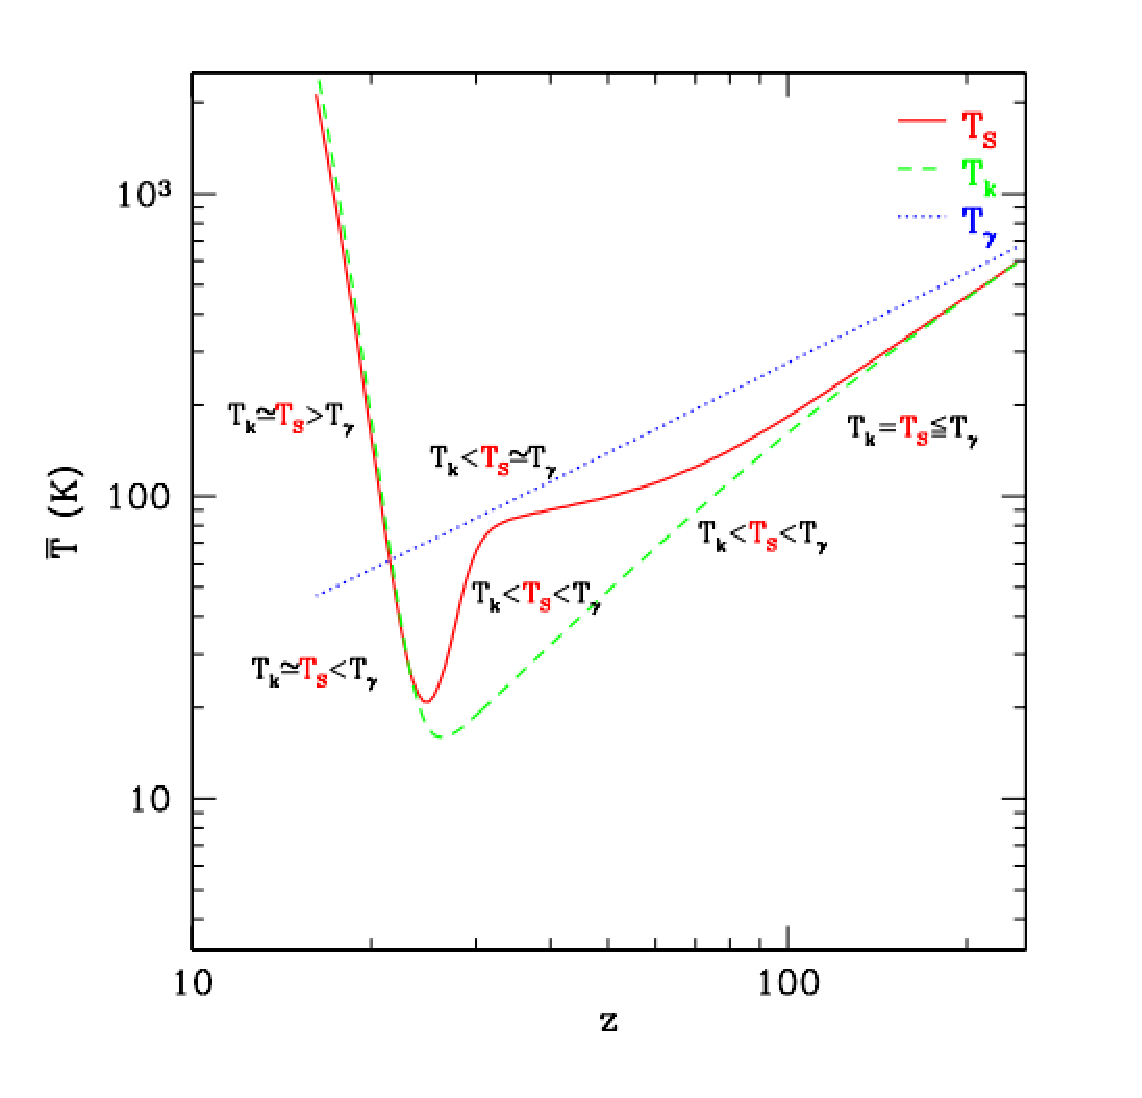
\includegraphics[width=90mm]{EoR/c03/c03.s1.f1.eps}
\centering
\caption{IGM$B29EY$N;~4V?J2=(B(\citep{2011MNRAS.411..955M})$B!#2#<4$O@VJ}JP0\!"=D<4$O29EY$rI=$9!#@V$$<B@~$O%9%T%s29EY!"NP$NGK@~$O%,%929EY!"@D$$E@@~$O(BCMB$B$N29EY$rI=$9!#(B}
\label{fig:igm_history}
\end{figure}

\begin{figure}[!h]
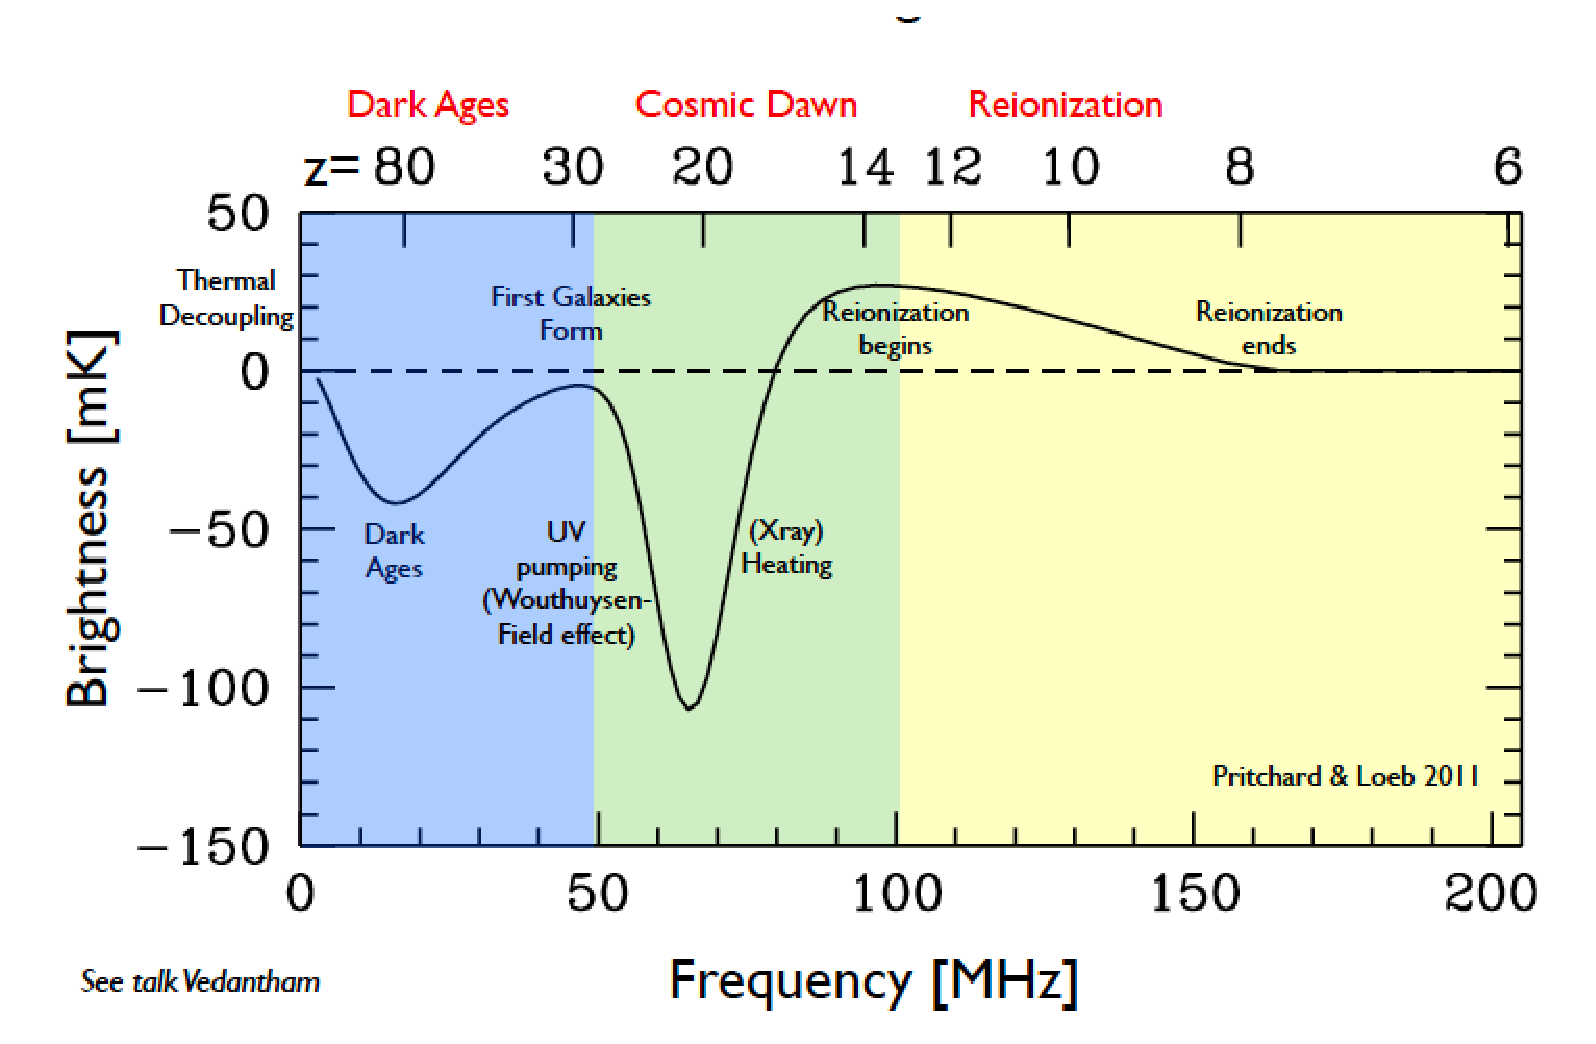
\includegraphics[width=105mm]{EoR/c03/c03.s1.f2.eps}
\centering
\caption{$B51EY29EY$N;~4VH/E8!J(BPritchard \& Loeb, 2011)$B!#2#<4$O<~GH?t!"=D(B
 $B<4$O51EY29EY!#(B$z\lesssim 30$$B$G=i4|E7BN$,7A@.$5$l$k$H!"$=$3$+$iH/$;$i$l(B
 $B$k;g308w$K$h$C$F(BWF$B8z2L$,5/$3$j!"%9%T%s29EY$O(BIGM$B$N%,%929EY$H%+%C%W%j%s%0(B
 $B$9$k!#$3$N$H$-!"%,%929EY$O(BCMB$B$N29EY$h$j>.$5$$$N$G!"51EY29EY$O5[<}@~$H$7(B
 $B$F8+$($k!#$7$+$7!"(B$z\sim 20$$B$G(BX$B@~$K$h$k2CG.$,8z$-;O$a$k$H!"%,%929EY$O5^(B
 $B7c$K>e>:$9$k$?$a!"(B$z\lesssim 15$$B$G$O!"51EY29EY$O51@~$H$7$F4QB,$5$l$k!#$^$?$3$N;~4|!":FEEN%$,;O$^$k!#(B$z\sim 8$$B$K$J$k$H!":FEEN%$,=*$o$j!"Cf@-?eAG$N3d9g$,#0$H$J$k$?$a!"51EY29EY$O<0(B(\ref{eq:brightness})$B$h$j#0$H$J$j!"51@~$b5[<}@~$b8+$($J$/$J$k!#(B}
\label{fig:delta_T}
\end{figure}

\subsubsection{(5) $16\lesssim z \lesssim 25$, $T_{\rm K}=T_{{\rm
S}}<T_{\gamma}$B"*(BT_{\rm K}=T_{{\rm S}}>T_{\gamma}$ (X$B@~$K$h$k2CG.4|(B)} 
WF$B8z2L(B
$B$K$h$j!"%,%9$N%9%T%s29EY$H%,%929EY$O6/$/%+%C%W%k$7$F$$$k$?$a!"1'ChKDD%$H(B
$B6&$K$=$NCM$O8:>/$7$F$$$/$,!"(BX$B@~$K$h$k2CG.$,8z$-;O$a$F$/$k$H!"NO3XE*29EY(B
$B$H%+%C%W%k$7$?%9%T%s29EY$O:G>.$NCM$KC#$7$?8e!"5^7c$J>e>:$r;O$a$k!#$3$N$H(B
$B$-!"1'Ch$NG.?J2=$NCf$G!"(BIGM$B$N29EY$,=i$a$F(BCMB$B8w;R$N29EY$h$j$b==J,Bg$-$/$J(B
$B$k$?$a!"(B$\delta T_{{\rm b}}>0$$B$G$"$k!#$7$?$,$C$F!"(BX$B@~$K$h$k2CG.0JA0$O!"(B
$B51EY29EY$NMI$i$.$O(BCMB$B8w;R$N29EY$KBP$9$k5[<}@~$H$7$F4QB,$5$l$k$,!"(BX$B@~2CG.(B
$B$,8z$-;O$a$k$H51@~$H$7$F4QB,$5$l$k;v$K$J$k!#(B


\subsubsection{(6) $7\lesssim z \lesssim 16$, $T_{\rm K}=T_{{\rm S}}\gg
   T_{\gamma}$ ($B:FEEN%4|(B)}
X$B@~$K(B
$B$h$k2CG.$,==J,$K8z$/$H!"<0!J(B\ref{eq:brightness}$B!K$h$j!"(B$\delta T_{{\rm
b}}$$B$O%9%T%s29EY$K0M$i$J$/$J$j!"29EY0MB8@-$r;}$?$J$/$J$k!#=i4|E7BN$+$i=P(B
$B$F$/$k%$%*%s2=%(%M%k%.!<$h$j$bBg$-$J%(%M%k%.!<$r;}$C$?8w;R$K$h$j!":FEEN%(B
$B$,;O$^$k$H!"%$%*%s2=NN0h!J(BHII$BNN0h!K$,A}$($F$$$-!"Cf@-?eAG$,@j$a$kNN0h(B
$B!J(BHI$BNN0h!K$O=y!9$K8:$C$F$$$/!#$3$l$K$h$j!"Cf@-?eAG$NNL$,8:>/$9$k$?$a!"(B
21cm$B@~$N%7%0%J%k$b8:>/$7$F$$$/!#:FEEN%4|$O!"(BHII$BNN0h$N?J2=$N;EJ}$d!"%$%*(B
$B%s2=8w;R$N?6$kIq$$!"%$%*%s2=8w;R$NJ|<M8;$N?6$kIq$$$J$I$K0MB8$9$k$N$G!"$3(B
$B$l$i$NFCD'$rD4$Y$kI,MW$,$"$k!#(B


$B0J>e!"(B(1)$B$+$i(B(6)$B$K<($7$?$N$,!"(BIGM$B29EY?J2=$N%"%&%H%i%$%s$G$"$j!"(BIGM$B29EY$O(B
$B?^(B\ref{fig:igm_history}$B$K<($9MM$J?6$kIq$$$r$9$k!#$^$?!"<B:]$N4QB,NL$G$"(B
$B$k51EY29EY(B($B<0(B\ref{eq:brightness})$B$N;~4VH/E8$r?^(B\ref{fig:delta_T}$B$K<($9!#(B
$B!!(B

\subsection{WF$B8z2L(B, X$B@~2CG.(B, $B:FEEN%$N%=!<%9(B}
$B$3$N@a$G$O!"(BWF$B8z2L!"(BX$B@~$K$h$k2CG.!":FEEN%$r0z$-5/$3$9E7BN$K$D$$$F=R$Y$k!#(B

\subsubsection{(1)$B<oB2(BIII$B@1(B $\&$ $B<oB2(BII$B@1(B}

$z\sim 30$$B$G!"=E85AG$r4^$^$:!"?eAG$GBgItJ,$,9=@.$5$l$?1'Ch:G=i$N@1$,7A@.(B
$B$5$l;O$a$k(B \citep{2006ApJ...652....6Y}$B!#$3$N$h$&$J?eAG86;R$N$_$G9=@.$5$l(B
$B$?@1$r<oB2(BIII$B@1$H8F$V!#6aG/$N%7%_%e%l!<%7%g%s$K4p$E$/8&5f$K$h$j!"<oB2(BIII
$B@1$O!"(B $BB@M[<ANL$N?t(B10$BG\DxEY$N<ANL$r;}$D$H9M$($i$l$F$$$k(B
\citep{2013RPPh...76k2901B}$B!#$3$N<oB2(BIII$B@1$+$iJ|<M$5$l$k%i%$%^%s(B$\alpha$
$B8w;R$K$h$C$F!"?eAG$N%9%T%s29EY$O%,%929EY$H%+%C%W%j%s%0$9$k!J(BWF$B8z2L!K!#<o(B
$BB2(BIII$B@1$+$i:n$i$l$k(BX$B@~O"@1$O!"(BIGM$B$N2CG.$rC4$&$b$N$H9M$($i$l$F$$(B $B$k(B
\citep{2014MNRAS.445..213F}$B!#$^$?!"<oB2(BIII$B@1$d>/NL$N=E85AG$r4^$`%,%9$+$i(B
$B7A@.$5$l$?<oB2(BII$B@1$,:FEEN%$r0z$-5/$3$9$H4|BT$5$l$F$$$k$,!"<oB2(BIII$B@1$N7A(B
$B@.2aDx!"$=$N8e$N<oB2(BII$B@17A@.%b!<%I$X$NA+0\2aDx$OL$$@Ff$,B?$$!#(B


\subsubsection{(2)Mini-quasar $\&$ AGN}
IGM$B$N2CG.$d:FEEN%$r0z$-5/$3$98w;R$N6!5k$N8;$H$7$F9M$($i$l$k$b$N$H$7$F!"(B
$BCf4V<ANL%V%i%C%/%[!<%k!J(BIMBH$B!K$d!"(BIMBH$B$X$N%,%9$N9_Ce$r5/8;$H$7$?(B
mini-quasar$B$,$"$k(B \citep{2007MNRAS.375.1269Z}$B!#$3$l$iE7BN$K$h$C$F0z$-5/(B
$B$3$5$l$k2CG.$d:FEEN%$O!"@1$+$i$N4sM?$KHf$Y$k$H>.$5$$$,!"(BCMB$B$N29EY$h$j$b(B
$B9b$$29EY$K(BIGM$B$r2CG.$9$k$N$K==J,$J%(%M%k%.!<$r;}$C$?8w;R$r@8@.$9$k$b$N$H(B
$B9M$($i$l$F$$$k!#$^$?!"(BIMBH$B$O8=:_$ND65pBg%V%i%C%/%[!<%k(B(SMBH)$B$N<o$K$J$C$F(B
$B$$$k2DG=@-$b$"$k$,!"%(%G%#%s%H%s9_CeN($h$j$b(B
$BBg$-$JCM$G9_Ce$r5/$3$5$J$1$l$P!"8=:_!"4QB,$5$l$F$$$k9b@VJ}JP0\$N(BAGN$B$N<A(B
$BNL$r@bL@$G$-$J$$$H$$$&LdBj$,$"$k!#(B

\subsubsection{(3) X-ray binaries}
$BA0=R$NDL$j!"<oB2(BIII$B@1M3Mh$N(BX$B@~O"@1$O(BIGM$B$N2CG.8;$H$7$FM-K>;k$5$l$F$$$k!#(B
$B$7$+$7!"(BX$B@~O"@1$O9b@VJ}JP0\$K$*$$$F!"Bg6IE*$J%9%1!<%k$r2CG.$9$k$N$K==J,(B
$B$J8D?t$,B8:_$7$F$$$?$N$+$H$$$&ITDj@-$,$"$k!#(B


\subsection{$B51EY29EY$rDL$7$?4QB,(B}
21cm$B@~$N4QB,$r9T$&$H$-!"2f!9$,<B:]$K1'ChO@E*!"E7BNJ*M}3XE*>pJs$r3MF@$9$k(B
$B$N$O!"51EY29EY$rDL$7$F$G$"$k!#$3$N>O$G$O!"51EY29EY$+$iF@$i$l$k>pJs$K$D$$(B
$B$F4J7i$K$^$H$a$k!#(B


\subsubsection{$B%Q%o!<%9%Z%/%H%k(B}
$B51EY29EY$NMI$i$.$r<h$j07$&$H$-!"$=$NE}7WNL$H$7$F!"0lHLE*$K9-$/MQ$$$i$l$F(B
$B$$$k$N$O$=$N%Q%o!<%9%Z%/%H%k$G$"$k!#0lHLE*$K%Q%o!<%9%Z%/%H%k$OGH?t$H@VJ}(B
$BJP0\$N4X?t$G$"$j!"%Q%o!<%9%Z%/%H%k$K$O!"51EY29EY$N%9%1!<%kKh$NMI$i$.$H$=(B
$B$N;~4VH/E8$N>pJs$,4^$^$l$F$$$k!#51EY29EY$NMI$i$.$r!"%P%j%*%s$NMI$i$.(B
$\delta_{b}$$B!"%$%*%s2=N($NMI$i$.(B $\delta_{x}$$B!"%i%$%^%s(B$\alpha$$B>l$NMI$i(B
$B$.(B $\delta_{\alpha}$$B!"(BIGM$B$N29EY$NMI$i$.(B$\delta_{T}$$B!"$5$i$KB.EY8{G[$NMI(B
$B$i$.(B $\delta_{\partial v}$$B$H!"3F!9$NMI$i$.$N78?t(B$\beta_{i}$$B$rMQ$$$k$H!"(B
$B<0(B(\ref{eq:fluctuation})$B$NMM$K=q$-2<$9;v$,$G$-$k(B
 \citep{2006PhR...433..181F}$B!#(B
\begin{equation}
\delta_{T_{b}}=\beta_{b}\delta_{b}+\beta_{x}\delta_{x}+\beta_{\alpha}\delta_{\alpha}+\beta_{T}\delta_{T}-\delta_{\partial v}
\label{eq:fluctuation}
\end{equation}
$B$3$NE83+$5$l$?MI$i$.$+$i!"$=$N%Q%o!<%9%Z%/%H%k$O!"(B
\begin{equation}
P_{T_{b}}(k,\mu)=P_{\mu^{0}}(k)+\mu^{2}P_{\mu^{2}}(k)+\mu^{4}P_{\mu^{4}}(k)
\label{eq:powerspectrum}
\end{equation}
$B$H7W;;$5$l$k!#(B$\mu$$B$O;k@~J}8~$HGH?t%Y%/%H%k$N$J$93QEY$NM>89$G$"$k!##19`L\$O!"%P%j%*%s$NMI$i$.!"%$%*%s2=N($NMI$i$.!"%i%$%^%s(B$\alpha$$B>l$NMI$i$.!"(BIGM$B$N29EY$NMI$i$.4V$G$N<+8JAj4X!"Aj8_Aj4X$r$^$H$a$?$b$N$G$"$k!#$9$J$o$A$3$l$O!"MI$i$.$NEyJ}@.J,$K$h$k%Q%o!<%9%Z%/%H%k$G$"$k!JB.EY8{G[$K$h$kMI$i$.$O%U!<%j%(6u4V$G9M$($k$H(B$\delta_{\partial v}$=$-\mu^{2}\delta$$B$H$J$k$?$a!"HsEyJ}E*$JMI$i$.$G$"$k!K!##29`L\$O!"HsEyJ}MI$i$.$G$"$kB.EY8{G[MI$i$.$HEyJ}MI$i$.$H$NAj8_Aj4X$K$h$k%Q%o!<%9%Z%/%H%k$r!"#39`L\$OHsEyJ}MI$i$.$K$h$k<+8JAj4X$K$h$k%Q%o!<%9%Z%/%H%k$rI=$7$F$$$k!#?^(B\ref{fig:igm_history_darkage}$B!"(B\ref{fig:igm_history_reionization}$B$K!"3F!9$N;~Be$N(B$\delta T_{{\rm b}}$$B$N%^%C%W$H%Q%o!<%9%Z%/%H%k$r<($9!#(B
%
\begin{figure}[htbp]
\centering
\includegraphics[width=125mm]{EoR/c03/c03.s1.f3a.eps}
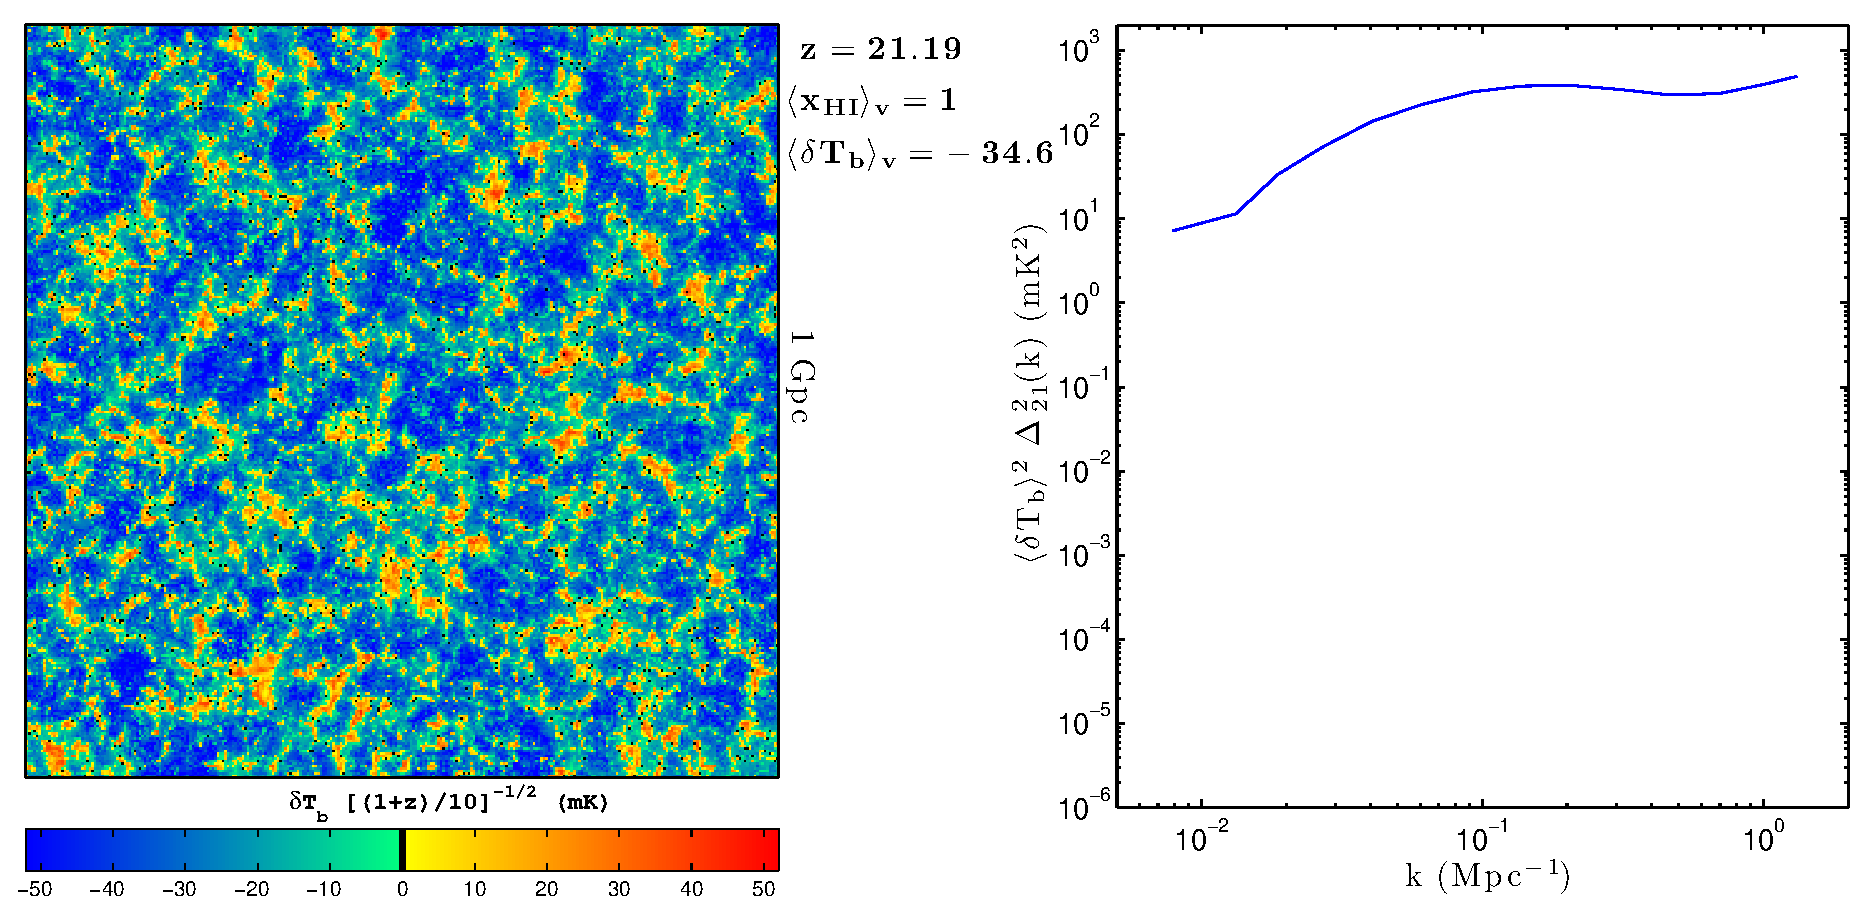
\includegraphics[width=125mm]{EoR/c03/c03.s1.f3b.eps}
\caption{$B%@!<%/%(%$%8!"(BCD$B$G$N(B$\delta T_{{\rm b}}$$B$N%^%C%W$H%Q%o!<%9%Z%/(B
 $B%H%k!J(BMesinger et al, 2010)$B!#:8$O(B$\delta T_{{\rm b}}$$B$N%^%C%W$G!"1&$,%Q(B
 $B%o!<%9%Z%/%H%k$N%0%i%U!#%Q%o!<%9%Z%/%H%k$N2#<4$OGH?t(B$k$$B$G=D<4$O%Q%o!<%9(B
 $B%Z%/%H%k!#%@!<%/%(%$%8=*HW$N(B$z$=30.07$B!"(BX$B@~$K$h$k2CG.$,==J,$K8z$/A0$N(B
 $z=21.19$$B$G$O!"51EY29EY$O(BCMB$B$KBP$9$k5[<}$H$7$F8+$($k!J(B$\delta T_{{\rm
 b}}<0$$B!K(B}
\label{fig:igm_history_darkage}
\end{figure}
%
\begin{figure}[htbp]
\includegraphics[width=125mm]{EoR/c03/c03.s1.f4a.eps}
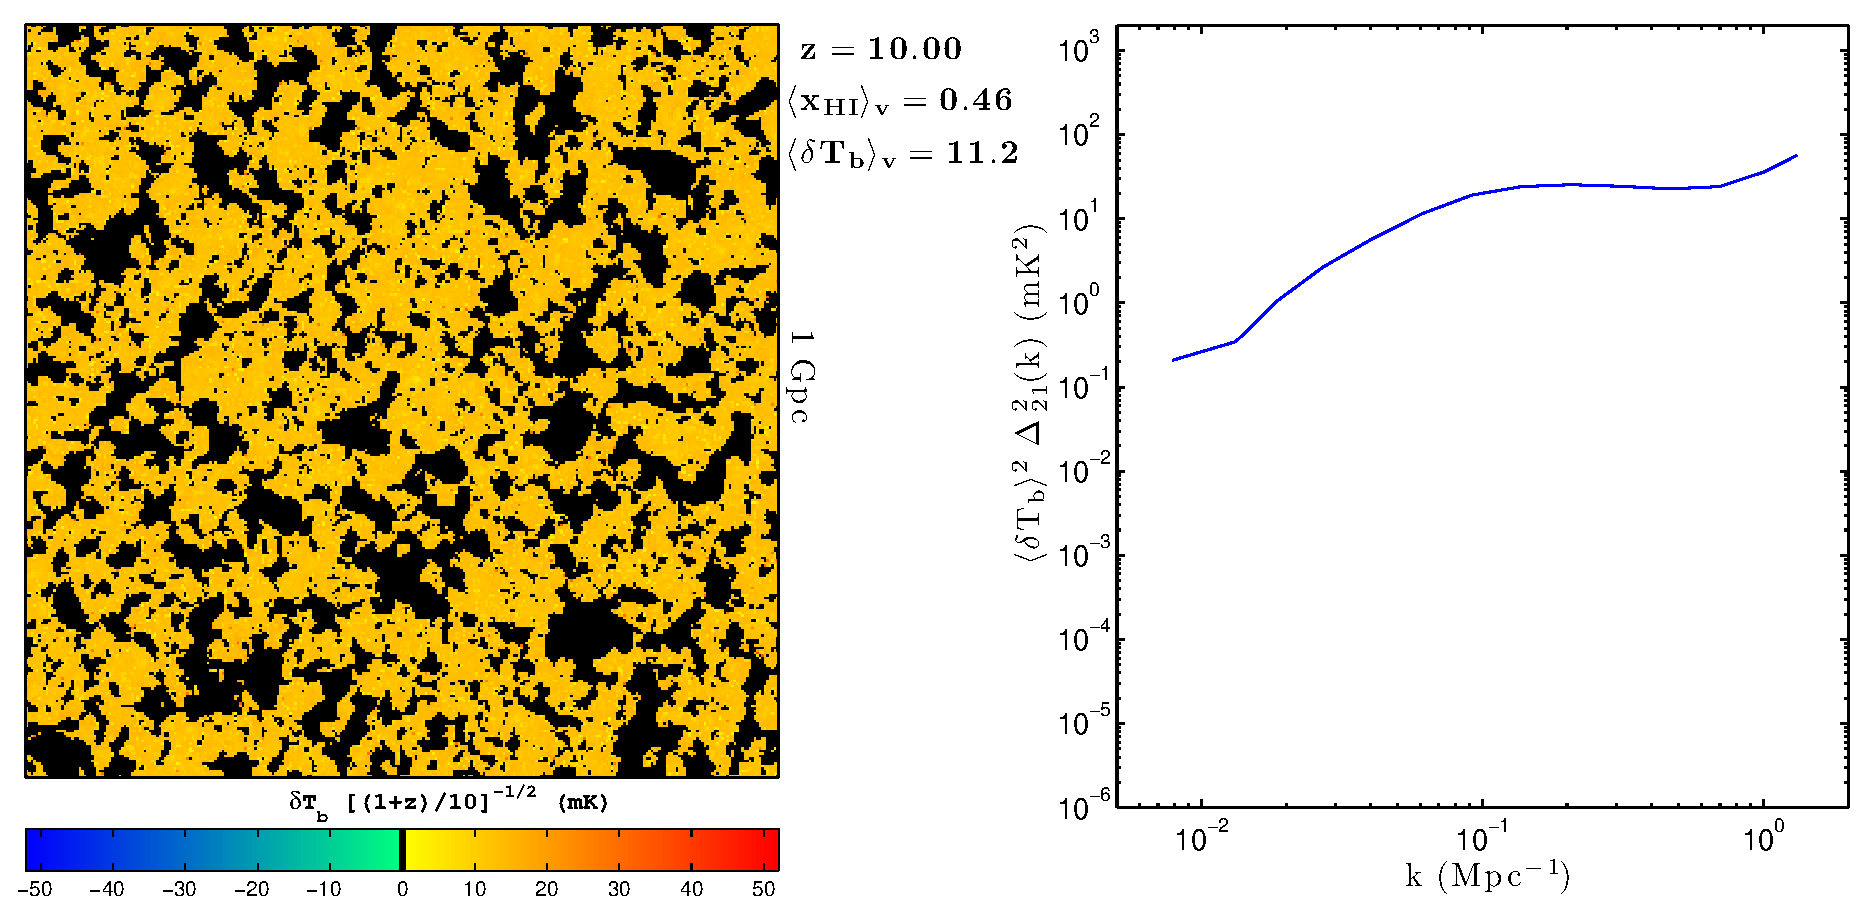
\includegraphics[width=125mm]{EoR/c03/c03.s1.f4b.eps}
\centering
\caption{$B:FEEN%4|$G$N(B$\delta T_{{\rm b}}$$B$N%^%C%W$H%Q%o!<%9%Z%/%H%k(B
 $B!J(BMesinger et al, 2010)$B!#2CG.$,==J,$K8z$$$F$$$k(B$z=17.94$$B$G$O!"51EY29EY(B
 $B$O51@~$H$7$F4QB,$5$l$k!J(B$\delta T_{{\rm b}}>0$$B!K!#$3$N$H$-!"?eAG$OCf@-(B
 $B>uBV$H$7$FB8:_$7$F$$$k$,!"(B$z=10.00$$B$K$J$k$H!":FEEN%$,;O$^$j!"?eAG$,%$%*(B
 $B%s2=$5$l$?NN0h$H!"Cf@->uBV$N$^$^$NNN0h$KJL$l$F$$$k$N$r8+$k;v$,$G$-$k!#(B
 $B%$%*%s2=NN0h$,%P%V%k$H$7$FI=$5$l!"Cf@->uBV$NItJ,$O%Q%C%A>u$K$J$C$F$*$j!"(B
 $BN><T$K$O6/$$%3%s%H%i%9%H$,$"$k!#(B}
\label{fig:igm_history_reionization}
\end{figure}

\subsubsection{$BB>$N4QB,NL(B}
$B%Q%o!<%9%Z%/%H%k0J30$K$b51EY29EY$+$iF@$i$l$k4QB,NL$H$7$F$O!"0J2<$N$b$N$,(B
$B5s$2$i$l$k!#(B
\begin{itemize}
\item $BJ,;6!"%b!<%a%s%H(B\\
      $B%Q%o!<%9%Z%/%H%k$,%U!<%j%(6u4V$GDj5A$5$l$kNL$G$"$k0lJ}$G!"<B6u4V>e$G$N51(B
      $BEY29EY>l$NE}7WE*@-<A$rC5$kJ}K!$H$7$F!"MI$i$.$NJ,;6$d9b<!$N%b!<%a%s(B
      $B%H(B($BODEY$d@mEY(B)$B$rMQ$$$kJ}K!$,$"$k!#EgB^$i$O%Q%o!<%9%Z%/%H%k$N;~4V0MB8@-$K(B
      $B$D$$$F!"51EY29EY$NJ,I[4X?t$NJ,;6$dODEY$KCmL\$7$F2r<a$rM?$($?(B
      \citep{Shimabukuro14}$B!#$3$l$K$h$k$H!"$I$N$h$&$JJ*M}%W%m%;%9$,(B
      $B%9%T%s29EY$r7h$a$F$$$k$+$K$h$C$FODEY$NId9f$,0[$J$j!"%Q%o!<%9%Z%/%H%k$N(B
      $B2r<a$r$9$k>e$GM-MQ$G$"$k!#(B
\item $B9b<!E}7WNL!"(B$n$$BE@Aj4X4X?t(B\\
      $B%U!<%j%(6u4V>e$N#2E@$r9M$($k$N$,%Q%o!<%9%Z%/%H%k$G$"$k0lJ}!"#3E@0J>e$r9M(B
      $B$($k9b<!E}7WNL$H$7$F!"%P%$%9%Z%/%H%k$,$"$k!#51EY29EY>l$NMI$i$.$,Hs(B
      $B%,%&%9J,I[$K=>$&>l9g!"%Q%o!<%9%Z%/%H%k$G$OC5$l$J$$>pJs$r%P%$%9%Z%/(B
      $B%H%k$O4^$s$G$$$k!#$^$?!"9b<!E}7WNL$r%U!<%j%(JQ49$7$F<B6u4V>e$G9M$((B
      $B$?$b$N$,(B$n$$BE@Aj4X4X?t$H$J$k!#5H1:$i$O(BSKA$B$d(Bpathfinder$B$N%P%$%9%Z%/%H%k$K(B
      $BBP$9$k46EY$r8+@Q$b$C$F$*$j!"(Bpathfinder$B$G$bBg%9%1!<%k(B
      $B!J(B$k \sim 0.1~{\rm Mpc^{-1}}$$B!K$G$"$l$P4QB,2DG=$G$"$k$3$H$r<($7$F$$$k!#(B
\item $B%H%b%0%i%U%#!<!"%$%a!<%8%s%0(B\\
      21cm$B@~$rMQ$$$?4QB,$G$O!"@VJ}JP0\Kh$N3,AXE*$J%^%C%W$N>pJs$r<j$KF~$l$k;v$,(B
      $B$G$-$k$N$G!"%H%b%0%i%U%#!<$r9M$($k;v$,$G$-$k!#$^$?!"%$%*%s2=%P%V%k(B
      $B$N?J2=$NMM;R$rC5$k<jK!$H$7$F!"51EY29EY$N6/EY$N6u4VE*J,I[$r4Q$k%$%a!<(B
      $B%8%s%0$,$"$k!#(B 
\item $B%$%*%s2=%P%V%k$dCf@-?eAGJ,I[$N%H%]%m%8!<(B\\
$B%$%*%s2=%P%V%k$dCf@-?eAGJ,I[$N4v2?3XE*$J>pJs$rC5$k<jK!$H$7$F!"%_%s%3%U%9(B
      $B%-!<HF4X?t$d%8!<%J%9E}7W$rMQ$$$kJ}K!$,$"$k!#(B 
\item $BGX7JEEGH8;$KBP$9$k(B21cm$B@~5[<}@~(B\\
      $BGX7JEEGH8;$+$iJ|<M$5$l$?EEGH$,(BIGM$B$d%_%K%O%m!<$K$h$k5[<}$r<u$1$k$H!"$=(B
      $B$NMM;R$O(B21cm$B@~$N5[<}@~$H$7$F4QB,$9$k;v$,$G$-$k!#(B 
\end{itemize}


\subsection{21cm$B@~%7%0%J%k$KBP$9$kA07JJ|<M(B}
$B$3$l$^$G8+$F$-$?$h$&$K!"(B21cm$B@~$O0E9u;~Be$+$i=iBeE7BN7A@.$r7P$F:FEEN%$^$G$N2aDx$rC5$k>e$G7hDjE*$K=EMW$JLr3d$r2L$?$9$H4|BT$5$l$k!#$7$+$7(B21cm$B@~%7%0%J%k$K$OB??t$=$7$F5pBg$JA07JJ|<M$,B8:_$7!"$3$l$r$J$s$i$+$NJ}K!$GHr$1$k$b$7$/$O:9$70z$+$J$1$l$P%7%0%J%k$rF@$k$3$H$O$G$-$J$$!#A07JJ|<M$O<g$K6d2O7OJ|<M$H7O30EEGHE7BN$N#2$D$KJ,$1$i$l!"0J2<$G6qBNE*$K@bL@$9$k!#(B

\paragraph{$B6d2O7OJ|<M(B}
$B6d2O7O$N%7%s%/%m%H%m%sJ|<M$H@)F0J|<M$O%7%0%J%k$KHf$Y$F05E]E*$KL@$k$/!"%Q%o!<%9%Z%/%H%k$K$*$$$F$O%7%0%J%k$N#67e0J>e$bBg$-$$!#$H$3$m$,N><T$H$b$K<~GH?t%9%Z%/%H%k$,Hs>o$K3j$i$+$G$"$k0lJ}!"%7%0%J%k$K$*$$$F$O%,%9L)EY$d%9%T%s29EY$N;k@~J}8~$K1h$C$?$f$i$.$rH?1G$7$F<~GH?t%9%Z%/%H%k$bBg$-$JJQF0$r;}$C$F$$$k$H4|BT$5$l$k!#$3$N$h$&$J@-<A$N0c$$$rMxMQ$7$F!"3F;k@~J}8~$KBP$7$F6d2O7OJ|<M$r8+@Q$b$C$F:9$70z$3$&$H$9$k;n$_$,9T$o$l$F$$$k!#<g$JJ}K!$H$7$F$O0J2<$N$h$&$JJ}K!$,5s$2$i$l$k(B\citep{Chapman15}$B!#(B
\begin{itemize}
\item $BB?9`<06a;w!'A07JJ|<M$N%9%Z%/%H%k$r<~GH?t$NDc<!$NB?9`<0$G$"$k$H2>Dj$7$F%U%#%C%H$7!"A07JJ|<M$r8+@Q$b$k!#$7$+$7<B:]$N%9%Z%/%H%k$,$I$N$h$&$J4X?t7A$K$J$C$F$$$k$+$o$+$i$:!"B?9`<0$N<!?t$r$$$/$D$K<h$k$+$K$h$C$F7k2L$,JQ$o$C$F$7$^$&$?$aG$0U@-$,$"$j!"8=:_$G$O$"$^$jM-MQ$JJ}K!$H$O9M$($i$l$F$$$J$$!#(B
\item Generalized Morphological Component Analysis$B!'A07JJ|<M$N%9%Z%/%H%k$,$"$k<o$N%7%s%W%k$5!J%9%Q!<%9@-!K$r;}$D$H$7$F?dDj$9$k!#6qBNE*$K$ONc$($P%9%Z%/%H%k$r%&%'!<%V%l%C%HJQ49$7$?;~$K$=$NE83+78?t$N$[$H$s$I$,%<%m$K$J$k$H2>Dj$9$k!#2r@O$KWs0U@-$,F~$i$J$$!#(B
\item Wp smoothing$B!'%9%Z%/%H%k$N6JN($NJQ2=$,$G$-$k$@$1>.$5$/$J$k$h$&$KA07JJ|<M$N4X?t7A$r8+@Q$b$k!#(B
\end{itemize}
$BB??t$NJ}K!$,Ds0F$5$l%7%_%e%l!<%7%g%s$,$5$l$F$$$k$,!"8=:_$N$H$3$m6d2O7OJ|<M=|5n$N7hDjBG$O$J$/!":#8e$NH/E8$,6/$/K>$^$l$F$$$k!#(B

\paragraph{$B7O30EEGHE7BN(B}
$B7O30$NEEGHE7BN$OE@8;$G$"$C$F$b43>D7WFCM-$N%S!<%`%Q%?!<%s$K$h$C$F<~0O$NNN0h$KO3$l=P$7$F$7$^$&!#$^$?;kLn$N9-$$K>1s6@$N>l9g$G$O!"Nc$(6d6KJ}8~$r4QB,$7$F$$$F$bBg$-$/9-$,$C$?%5%$%I%m!<%V$rDL$7$F6d2OLLJ|<M$,F~$j9~$s$G$/$k!#$3$l$i$rHr$1$k$?$a$K$OE75eLL>e$N$I$N0LCV$K$I$N$h$&$JL@$k$5$NE7BN$,B8:_$9$k$+$r5-=R$9$k%9%+%$%b%G%k$r@53N$K9=C[$7!"%S!<%`$N7A>u$b@53N$KM}2r$9$k$3$H$K$h$C$F4QB,%G!<%?$r3S@5$9$kI,MW$,$"$k!#$^$?CO5e$NEEN%7w$b%9%+%$%b%G%k$K1F6A$9$k$,!"EEN%7w$O;~!99o!9$HJQ2=$7!"$5$i$K43>D7W$N4p@~D9$,D9$$$H1F6A$r<u$1$kEEN%7w$N0LCV$,K>1s6@$4$H$K0[$J$k$?$a3S@5$O$h$j:$Fq$K$J$k!#(B

\paragraph{$B7W;;%3%9%H(B}
$BA07JJ|<M=|5n$N0lHLE*$J<jB3$-$H$7$F$O!"7O30$NEEGHE7BN$r3S@5$7$?8e!";k@~$4$H$K6d2O7OJ|<M$r=|5n$9$k$3$H$K$J$k!#@h$K=R$Y$?$h$&$KEEN%7w$O;~!99o!9$HJQ2=$9$k$?$a!"C;;~4V$N@QJ,$4$H$K3S@5$O9T$o$l$k!#$=$N$?$a3S@5$H6d2O7OJ|<M$N=|5n$K$OB?Bg$J7W;;%3%9%H$,$+$+$k$3$H$K$J$j!"$3$l$i$OC1$K@53N$J$@$1$G$J$/7W;;%3%9%H$b$*$5$($k$h$&$K$J$5$l$J$1$l$P$J$i$J$$!#$3$NE@$b:#8e$N2]Bj$G$"$k!#(B


\subsection{$B8=:_$N@)8B(B}
$B:FEEN%4|$KBP$9$k4QB,$O$3$l$^$G$K$b9T$o$l$F$*$j!"$=$l$K$h$C$F:FEEN%;K$d$=$l$K4XO"$9$k9b@VJ}JP0\$G$N@17A@.;K$KBP$9$k@)8B$,F@$i$l$F$$$k!#$3$N@a$G$O!"8=:_!":FEEN%4|$K$D$$$F4QB,E*$K$I$N$h$&$J@)8B$,$5$l$F$$$k$N$+=R$Y$k!#(B

$B$?$@$7!"8=:_F@$i$l$F$$$k$N$O:FEEN%4|=*N;4V:](B$(z\lesssim 10)$$B$N>pJs$@$1$G$"$j!":FEEN%3+;O;~4|$NJ*M}$O0MA3$H$7$FJ,$+$C$F$$$J$$$?$a!":#8e$N4QB,$NH/E8$,4|BT$5$l$k!#(B

\subsubsection{$B%,%s(B-$B%T!<%?!<%=%s$NC+(B}
$B9b@VJ}JP0\$G8+$D$+$C$?%/%(!<%5!<$N%9%Z%/%H%k$r8+$k$3$H$G!":FEEN%$N40N;$7(B
$B$?;~4|$r8+@Q$b$k$3$H$,$G$-$k!#1'Ch$KCf@-?eAG$,K~$A$F$$$k$H$-$O!"9b@VJ}JP(B
$B0\$N%/%(!<%5!<$+$iJ|<M$5$l$?%i%$%^%s(B$\alpha$$B8w;R$O!"Cf@-?eAG$K$h$C$F5[<}(B
$B$5$l$k!#$3$N$H$-!"2f!9$O!"1'ChKDD%$K$h$k@VJ}JP0\$K$h$C$F0z$-1d$P$5$l$?%i(B
$B%$%^%s(B$\alpha$$B8w;R$NGHD9$G!"5[<}@~%9%Z%/%H%k$r4QB,$9$k$3$H$,$G$-$k!#$^$?!"(B
$B%/%(!<%5!<$+$iJ|<M$5$l$?%i%$%^%s(B$\alpha$$B$h$j$bGHD9$NC;$$8w$O!"1'ChKDD%$K(B
$BH<$&@VJ}JP0\$N8z2L$K$h$C$F%i%$%^%s(B$\alpha$$B$NGHD9$K$J$j!"BP1~$9$k@VJ}JP0\(B
$B$NCf@-?eAG$K5[<}$5$l$k!#:FEEN%$,40N;$K6a$E$/$K$D$l!"Cf@-?eAG$,$J$/$J$k$?(B
$B$a!"5[<}@~%9%Z%/%H%k$,8+$($K$/$/$J$k!#$3$l$K$h$j!":FEEN%4|$N=*N;;~4|$r8+(B
$B@Q$b$k$3$H$,$G$-$k!#4QB,%9%Z%/%H%k$K9o$^$l$?5[<}@~$NO"$J$j$r%,%s(B-$B%T!<%?!<(B
$B%=%s$NC+$H8F$V!#$3$NJ}K!$K$h$C$F!"(B$z\sim6$$B$G:FEEN%$,=*N;$7$?;v$,$o$+$C$F(B
$B$$$k(B \citep{2006AJ....132..117F,2011Natur.474..616M}$B!#(B

\subsubsection{CMB$B;6Mp$N8w3XE*8|$_(B}
CMB$B8w;R$H:FEEN%4|$N%$%*%s2=%P%V%kCf$NEE;R$H$N;6Mp$K$h$C$F!"(BCMB$B$N%Q%o!<%9(B
$B%Z%/%H%k$KJP8w$K$h$k$f$i$.$,2C$o$j!"%9%Z%/%H%k$,JQ2=$9$k!#$=$3$+$i:FEEN%(B
$B$N4|4V$d%$%*%s2=N($NMI$i$.$J$I$K@)8B$rF@$k$3$H$,$G$-$k!#8=:_!"(BCMB$B$N;6Mp(B
$B$O(B$z\sim10$$B$G5/$3$j!"$=$N$H$-;6Mp$N8w3XE*8|$_$,(B$\tau\sim0.09$$BDxEY$G$"$k(B
$B;v$,J,$+$C$F$$$k(B \citep{2013arXiv1303.5081P}$B!#(B

\subsubsection{IGM$B29EY(B}
$z\approx 6$$B$N%/%(!<%5!<$N<~0O$N%,%929EY$r%U%)!<%/%H%W%m%U%!%$%kJ,@O(B($BJ,I[(B
$B$r%U%)!<%/%H4X?t$G%U%#%C%F%#%s%0(B)$B$K$h$C$FB,$j!"$=$l$H:FEEN%4|$G$N%/%(!<%5!<(B
$B<~JU$N@:L)$J%7%_%e%l!<%7%g%s$rHf3S$9$k$3$H$G!":FEEN%4|$N%,%929EY?J2=;K$K(B
$B@)8B$r2C$($k$3$H$,$G$-$k!#$3$l$K$h$l$P!"(BH\textsc{i}$B$NEEN%$O!"(B$z\lesssim
11$$B$G5/$3$C$?$H4|BT$5$l$k(B \citep{2010MNRAS.406..612B}$B!#(B

\subsubsection{$B%,%s%^@~%P!<%9%H(B}
$B%,%s%^@~%P!<%9%H(B(GRBs)$B$OBg<ANL@1$ND6?7@1GzH/$HL)@\$K4X78$7$F$$$k$H9M$($i(B
$B$l$F$$$k!#$7$?$,$C$F!"9b@VJ}JP0\$G(BGRBs$B$,4QB,$5$l$F$$$k;v<B$O!"1'Ch$N=i4|(B
$B$KBg<ANL@1$,B8:_$7$?2DG=@-$r<($7$F$$$k!#$3$l$K$h$j!":#8e$h$jB?$/$N9b@VJ}(B
$BJP0\(BGRBs$B$,4QB,$5$l$l$P!":FEEN%4|0JA0$NBg<ANL@1$N@17A@.N($K@)8B$r2C$($k$3(B
$B$H$,$G$-$k(B \citep{2009Natur.461.1254T}$B!#$^$?!"9b@VJ}JP0\(B GRBs$B$N0lIt$O%i(B
$B%$%^%s(B$\alpha$$B8:?jMc$N%U%#%C%F%#%s%0$K$h$k:FEEN%4|$NCf@-?eAG3d9g$N@)8B$K(B
$B$bMQ$$$i$l$F$$$k(B (e.g.,\cite{2006PASJ...58..485T}$B!#(B


\subsubsection{$B9b@VJ}JT0\6d2O(B}
$B9b@VJ}JT0\$G$NCf@-?eAG$K$h$k6/$$5[<}$r<u$1!"4QB,$5$l$F$$$J$$%I%m%C%W%"%&(B
$B%H6d2O$N4QB,$+$i!"@17A@.;K$K@)8B$r2C$($k$3$H$,$G$-$k!#8=:_$N4QB,$+$i$O!"(B
$z>10$$B$G5^7c$K@17A@.N($,2<$,$C$F$$$k;v$,<(:6$5$l$F$$$k(B
(\citep{2013ApJ...773...75O})$B!#$^$?!"(B$z>6$$B$N%i%$%^%s(B$\alpha$$B51@~6d2O$N8D(B
$B?tL)EY$O!"9b@VJ}JT0\$[$I>.$5$/$J$C$F$*$j!"$3$l$OCf@-?eAG$K$h$k8:8w$K5/0x(B
$B$9$k$H$b9M$($i$l$F$$$k(B (e.g.,\cite{2010ApJ...723..869O})$B!#(B


\subsubsection{$B6a@V30@~(B}
$B1'Ch=i4|$N6d2O$d@1$+$iJ|<M$5$l$?(BUV$B$O;d$?$A$,4QB,$9$k$^$G$K!"6a@V30$N<~GH(B
$B?t$^$G@VJ}JP0\$9$k!#$=$N6/EY$dHsEyJ}@-$+$i!"1'Ch=i4|$G$N;g30@~8;$NJ,I[$d(B
$BB8:_NLEy$N@-<A$K@)8B$,IU$1$i$l$k2DG=@-$,$"$k!#%Q%o!<%9%Z%/%H%k$KBP$9$k>e(B
$B8B$O$"$k$b$N$N!"M}O@CM$rBgI}$K>e2s$C$F$$$k(B \citep{2012ApJ...756...92C}$B!#(B
\subsubsection{X$B@~(B}
$BFp(BX$B@~(B(Soft X-ray)$BGX7JJ|<M6/EY$r4QB,$9$k$3$H$G!"?eAG86;R(B1$B8D$"$?$j$N(BX$B@~8w(B
$B;R?t$K@)8B$r2C$($k$3$H$,$G$-$k!#$5$i$K$=$3$+$i!"(BX$B@~$N%=!<%9$r@)8B$G$-$k!#(B
$BNc$($P(B$z=10$$BIU6a$N4QB,E*@)8B$K$h$k$H!"Bg<ANL(BX$B@~O"@1$H%@!<%/%^%?!<BP>CLG(B
$B$K$h$k?eAG86;R$"$?$j$N8w;R?t$O(B0.1$BDxEY$7$+L5$$$3$H$,$o$+$C$F$$$k!#$^$?!"(B
$B3hF06d2O3K(B(AGN)$B$O:FEEN%$K:GBg(B10\%$BDxEY$7$+4sM?$G$-$J$$$3$H$bJ,$+$C$F$$$k(B 
\citep{2012MNRAS.426.1349M}$B!#(B 



\subsubsection{SKA$B%Q%9%U%!%$%s%@!<(B}
SKA$B$N40@.$O$^$@$^$@1s$$$,!"8=:_(BSKA$B40@.$^$G$N;n83$d4QB,E*<B83$H$7$F$$$/$D(B
$B$+K>1s6@$,7z@_$5$l!"4QB,$,9T$o$l$F$$$k!#$=$l$i$N4QB,$+$i$b:FEEN%4|$N(B21cm
$B%Q%o!<%9%Z%/%H%k$KBP$9$k@)8B$,F@$i$l$F$$$k!#$3$3$G$O!"3FK>1s6@$H4QB,7k2L(B
$B$K$D$$$F4JC1$K?($l$k!#(B 

\subsubsection{GMRT}
GMRT(Giant Metrewave Radio Telescope)$B$O%$%s%I$K$"$k!#J,2rG=$O(B20$BIC3Q!":G(B
$B$bDc$$<~GH?tBS$,(B139.3$\sim$156.0MHz$B$r%+%P!<$7$F$*$j!"(B$z=8.1\sim9.2$$B$r8+(B
$B$k$3$H$,$G$-$k!#(B$z\sim8.8$$BIU6a$N%Q%o!<%9%Z%/%H%k$K$D$$$F$N>e8B$,F@$i$l$F(B
$B$$$k(B \citep{2013MNRAS.433..639P}$B!#(B

\subsubsection{MWA}
MWA(Murchison Widefield Array)$B%*!<%9%H%i%j%"$K@_CV$5$l$F$$$k!#(B128$B8D$N%"(B
$B%s%F%J$+$i@.$C$F$$$k!#(B2$BJ,3Q$NJ,2rG=$r;}$A!"<~GH?t(B80$\sim$300MHz$B$r4QB,2D(B
$BG=$G$"$k!#(Bz=9.5$B$NGH?t(Bk=0.046$\rm Mpc^{-1}$$B$G%Q%o!<%9%Z%/%H%k$NJ?J}:,$,(B
0.3K$B$h$j>.$5$$$H$$$&@)8B$rF@$F$$$k(B \citep{2014PhRvD..89b3002D})$B!#(B

\subsubsection{PAPER}
PAPER(Precision Array for Probing the Epoch of Reionization)$B$OFn%"%U%j%+(B
$B$K@_CV$5$l$F$$$k!#(B32$B$N%"%s%F%J$+$i@.$C$F$$$k!#%Q%o!<%9%Z%/%H%k$KBP$7$F!"(B
z=7.7$B$G(Bk=0.11h$\rm Mpc^{-1}$$B$G>e8B(B2704$\rm mK^{2}$$B$rM?$($k(B \citep{2014ApJ...788..106P}$B!#(B
\subsubsection{LOFAR}
LOFAR(LOw Frequency ARray)$B$O%*%i%s%@KLIt$rCf?4$H$7$F!"9-0h$K%"%s%F%J$rG[(B
$BCV$7$F!"$=$l$i$r0l$D$NEEGH43>D7W$H$7$F07$&!#$=$ND>7B$O(B100km$B$K$b$N$\$j!"(B
$B<~GH?t$O(B10$\sim$250MHz$B$,4QB,2DG=$G$"$k(B\citep{2013A&A...556A...2V}$B!#(B



%未解決のサイエンス


\input{EoR/EoR.s2.tex}
%\setcounter{section}{3}
\section{日本が狙うサイエンス}\label{c03.s3}
$B1'Ch$N:FEEN%$,$I$N$h$&$K$7$F5/$3$C$?$+!"$H$$$&LdBj$OM}O@E*$K$b4QB,E*$K$b(B
$BL$$@L@$i$+$K$5$l$F$$$J$$8&5f%F!<%^$G$"$k!#4QB,E*$K$O!":#8e(BSquare
Kilometre Array (SKA)$B$KBeI=$5$l$kBg7?$NDc<~GHEEGH43>D7W$K$h$j!"1sJ}1'Ch$G(B
$B$NCf@-?eAG(B21 cm$B@~4QB,$,Bg$-$/?JE8$9$k$3$H$,4|BT$5$l$F$$$k!#$=$3$G(BSKA-JP $B:F(B
$BEEN%HI$G$O!"F@$i$l$kKDBg$J4QB,%G!<%?$+$i1'Ch:FEEN%4|$K5/$-$?8=>]$rM}2r$9(B
$B$k$?$a$K!"4QB,%G!<%?$H$NHf3S$KBQ$($kM}O@%b%G%k$N9=C[$*$h$S4QB,E*M=8@$r9T(B
$B$&!#$^$?!"1sJ}1'Ch$N>pJs$rF@$k$?$a$K$OA07JJ|<M!"$H$/$K7O30$N%3%s%Q%/%H$J(B
$BEEGH8;$d7OFb$N%7%s%/%m%H%m%sJ|<M$,LdBj$K$J$k$H;XE&$5$l$F$$$k$3$H$+$i!"4{(B
$BB8$N4QB,AuCV$rMQ$$$F!"$3$l$i$N=|5n!&2sHr$K$D$$$F<B>ZE*$K8&5f$9$k!#(B

$B$9$J$o$A!"1'Ch:FEEN%4|$N>pJs$r==J,$K3hMQ$G$-$k$h$&$K$9$k$?$a!"(BSKA-JP $B:F(B
$BEEN%HI$G$O0J2<$NFs$D$r3hF0$NCl$H$9$k!#(B

\begin{itemize}
 \item[(1)] $BB.$/@53N$JM}O@%b%G%k7W;;$r9T$&7W;;%3!<%I$N3+H/(B
 \item[(2)] $BDc<~GHNN0h$NA07JJ|<M$N%b%G%k2=$H=|5nJ}K!$N9=C[(B
\end{itemize}

$B0J2<$G$O!"$^$:4{B8$N7W;;%3!<%I(B21cmFAST$B$N>\:Y$r5-$7!"(B
$B$=$NLdBjE@$r;XE&$7$?$N$A!"(BSKA-JP$B$N@oN,$r5-=R$9$k!#(B

\subsection{$B4{B8$N7W;;<jK!!J(B21cmFAST$B$rNc$K$7$F!K(B\label{sec.21cmFAST}}
$B8=:_MxMQ2DG=$J1'Ch:FEEN%4|$N=`2r@OE*$J7W;;%3!<%I$O(BSimFast21(\citep{2010ascl.soft10025S})$B$d(B21cmFAST(\citep{2011MNRAS.411..955M})$B$,$"$k!#$3$l$i$N7W;;%3!<%I$O(B
$B%$%*%s2=$dL)EY?J2=Ey$rMM!9$J6a;w$rMQ$$$F7W;;$7!"J#;($J1'Ch:FEEN%4|$NMM;R(B
$B$r:F8=$7$h$&$H$9$k$b$N$G$"$k!#(B

21cmFAST$B$O(B21cm$B@~51EY29EY$N;0<!85%^%C%W$r7W;;$9$k;v$,$G$-$k!#(B21cmFAST$B$N%3!<(B
$B%IFb$G(B21cm$B@~$N51EY29EY$O(B(3.1)$B<0$G7W;;$5$l$k!#(B 
\begin{eqnarray}
{\delta}T_{b}(\nu)&=&\frac{T_{s}-T_{\gamma}}{1+z}(1-e^{-\tau_{\nu_{0}}})\nonumber\\
  &\approx&27x_{{\rm HI}}(1+\delta_{m})\left(\frac{H}{dv_{r}/dr+H}\right)\left(1-\frac{T_{\gamma}}{T_{s}}\right)\left(\frac{1+z}{10}\frac{0.15}{\Omega_{m}h^{2}}\right)^{\frac{1}{2}}\left(\frac{\Omega_{b}h^{2}}{0.023}\right)[\rm mK]
\end{eqnarray}
$B%P%j%*%s$NL)EYMI$i$.(B$\delta_m$$B!"Cf@-N((B$x_{{\rm HI}}$$B!"%9%T%s29EY(B$T_s$$B!"(B
$BB.EY8{G[(B$dv_r/dr$$B$G$"$k!#$^$:!"$3$l$i#4$D$NNL$,#3<!85$N%^%C%W$H$7$F7W;;(B
$B$5$l!"$=$l$i$rMQ$$$F51EY29EY$N%^%C%W$r7W;;$9$k!#(B 
$B0J2<$G$O$^$:!"(B21cmFAST$B$G$3$l$i$NNL$r$I$N$h$&$K7W;;$7$F$$$k$+$^$H$a$k!#(B 

$B$^$:!"L)EY>l$K$D$$$F!#L)EY>l$N7W;;$O%<%k%I%S%C%A6a;w$rMQ$$$F9T$o$l$k!#(B
$BL)EY$N>pJs$O;0<!85$N%^%C%W$N%;%k$4$H$KM?$($i$l$k!#$3$NL)EY>l$N>pJs$r$b$H(B
$B$K;D$j$N#3$D$NNL$O7W;;$5$l$k!#(B 
$BF@$i$l$?L)EY>l$N%^%C%W$+$i!"%$%*%s2=N((B$x_{{\rm HII}}$$B$N7W;;$r9T$&!#Cf@-N($O(B$x_{{\rm HI}}=1-x_{{\rm HII}}$$B$G$"$k!#(B
21cmFAST$B$GMQ$$$i$l$F$$$k%$%*%s2=$NH=Dj$N<0$O3FE@(B$x$$B$H3F@VJ}JP0\(B$z$$B$K$*$$$F<!$N$h$&$K=q$1$k!#(B
\begin{eqnarray} 
f_{coll}(x,z,R)\geq\zeta^{-1}
\end{eqnarray}
$\zeta$$B$O%$%*%s2=8zN($H8@$C$F!"6d2O$,<~0O$NJ*<A$r%$%*%s2=$9$k8zN($rI=$9!#(B
$B%$%*%s2=$NH=Dj$G$O$^$:!"$"$k%;%k$N<~0O$KH>7B(B$R$$B$N5e$r9M$($k!#$3$N(B$R$$B$O%$%*%s2=8w;R$NJ?6Q<+M39TDx$KBP1~$7!"(B21cmFAST$B$G$O%Q%i%a!<%?$H$7$FDj?t$GM?$($i$l$k!#$3$N5eCf$NJx2uHf(B $f_{coll}$$B$r7W;;$7$F>e<0$KEv$F$O$a$k!#(B$f_{coll}$$B$O5eA4BN$N<ANLL)EY$H!"5eCf$G==J,$KJx2u$7$?<ANLL)EY$NAmOB$H$NHf$G$"$k!#>r7o$rK~$?$7$F$$$k$J$i!"$=$N%;%k$K$O%$%*%s2=$9$k$N$K==J,$JNL$N8w;R$,B8:_$9$k$H$7$F%$%*%s2=$7$?$H$_$J$7!"Cf@-N($r(B0$B$H$9$k!#>r7o$rK~$?$7$F$$$J$$>l9g!"5e$NH>7B$r=L$a$FF1MM$NA`:n$r9T$&!#>r7o$rK~$?$9$^$G7+$jJV$7!":G>.$N(B$R$(1grid$B$NBg$-$5(B)$B$^$G>r7o$,K~$?$5$l$J$+$C$?>l9g!"$=$N%;%k$N%$%*%s2=N($O(B$\zeta f_{coll}$$B$H$9$k!#$3$NA`:n$rA4%;%k$KBP$7$F9T$&!#(B

$B%9%T%s29EY$O:FEEN%0JA0$N51EY29EY$GFC$K=EMW$K$J$k!#$^$?!"(B21cmFAST$B$N7W;;$NCf$G:G$bJ#;($G;~4V$N$+$+$kItJ,$G$"$k!#%9%T%s29EY$N7W;;$O(B(3.2)$B<0$G9T$o$l$k!#(B
\begin{equation}
T_S^{-1}=\frac{T_{\gamma}^{-1}+x_{\alpha}T_{\alpha}^{-1}+x_cT_K^{-1}}{1+x_c+x_{\alpha}}\nonumber
\end{equation}
$T_{\gamma}$$B$O(BCMB$B29EY!"(B$T_K$$B$O%,%929EY$G$"$k!#(B$T_{\alpha}$$B$O(BLyman-$\alpha$$B?'29EY$G$"$k$,!"(B$T_{\alpha}=T_K$$B$H$$$&6a;w$rMQ$$$k$N$G<B:]$K$O%,%929EY$r7W;;$9$k!#(B
$x_c$$B$O>WFM78?t$G$"$k!#7W;;<0$O(B
\begin{equation}
x_c=\frac{0.0628 K}{A_{10}T_{\gamma}}[n_{{\rm HI}}\kappa^{HH}_{1-0}(T_K)+n_{e}\kappa^{eH}_{1-0}(T_K)+n_{p}\kappa^{pH}_{1-0}(T_K)]
\end{equation}
$B$H$J$k!#(B$A_{10}$$B$O<+A3J|<M78?t$G$"$k!#E:;z$O(B(${\rm HI},e,p$)=($BCf@-?eAG(B,$BEE;R(B,$BM[;R(B)$B$rI=$7$F$$$k!#(B$n_i$$B$O$=$l$>$l$N?tL)EY$G$"$k!#(B$\kappa$$B$O%,%929EY$K0MB8$9$k>WFM8zN($G$"$j!"BP1~$9$k?tCM$,MQ0U$5$l$F$$$k!#(B
$B%,%929EY$N7W;;$O<!$N<0$rMQ$$$k!#(B
\begin{equation}
\frac{dT_K({\bf{x}},z')}{dz'}=\frac{2}{3k_B(1+x_e)}\frac{dt}{dz'}\sum_p\epsilon_p+\frac{2T_K}{1+z'}
+\frac{2T_K}{3}\frac{dD(z')/dz'}{D(z)/\delta_{nl}({\bf{x}},z)+D{z'}}
-\frac{T_K}{1+x_e}\frac{dx_e}{dz'}
\label{TK}
\end{equation}
$B$H$J$k!#<0(B(\ref{TK})$B$NBh0l9`$OMM!9$J%W%m%;%9$N2CG.$N8z2L$G(B$\epsilon_p$$B$O$"$k2aDx(B($p$)$B$G$N2CG.N($rI=$9!#BhFs9`$O%O%C%V%kKDD%$N8z2L!"Bh;09`$O9=B$7A@.$KH<$&CGG.E*$J2CG.$HNd5Q$N8z2L!"Bh;M9`$O%$%*%s2=$K$h$k%,%9N3;R?t$NJQ2=$rI=$9!#(B
$B2CG.$N%W%m%;%9$O%3%s%W%H%s;6Mp$H(BX$B@~J|<M$r9MN8$9$k!#(B
X$B@~J|<M$K$h$k2CG.$N7W;;$O%^%C%W$N3F%;%k$4$H$K9T$o$l$k!#6qBNE*$K$O!"%;%k$rCf?4$K5e3L$r9M$($k!#$=$N5e3LCf$G(B$f_{coll}$$B$r7W;;$7!"9M$($F$$$k%;%k$KE~C#$9$k(BX$B@~$NJ|<M8w;R$NNL$r8+@Q$b$k!#$3$N:]!"==J,1sJ}$+$i$N(BX$B@~J|<M$N4sM?$r8+@Q$b$k$?$a!"@VJ}JP0\(B$z$$B$K4X$9$k@QJ,$G7W;;$5$l$k!#(B

$x_{\alpha}$$B$O(BLyman-${\alpha}$$B9`8w;R$H$N>WFM78?t$G$"$j!"<!$N$h$&$K=q$1$k!#(B
\begin{equation}
x_{\alpha}=1.7\times10^{11}(1+z)^{-1}S_{\alpha}J_{\alpha}
\end{equation}
$B$3$3$G(B$S_{\alpha}$$B$O86;RJ*M}$r9MN8$7$?=$@578?t!"(B$J_{\alpha}$$B$O(BLyman-$\alpha$$B$NGX7JJ|<M$G$"$k!#(B
Lyman-$\alpha$$B$NGX7JJ|<M$O#2$D$N4sM?$r7W;;$9$k!#0l$D$O(BX$B@~$K$h$C$FNe5/$5$;$i$l$?(BHI$B$+$i$NJ|<M$G!"(BX$B@~$K$h$k2CG.$HF1MM$K5e3L$+$i%;%k$X$N4sM?$r7W;;$9$k!#$b$&0l$D$O@1$+$iJ|<M$5$l$?(BLyman-n$B8w;R$,(BLyman-$\alpha$$B$K%+%9%1!<%I$9$k8z2L$G$"$k!#$3$A$i$b5e3L$+$i$N4sM?$r9M$($k!#(B
$B$^$?!"B.EY8{G[$K$D$$$F$O3F%;%k$NL)EY>l$H@~7A@.D90x;R(B$D(z)$$B$N;~4VHyJ,$rMQ$$$F<!$N<0$G7W;;$5$l$k!#$?$@$7!"$3$N9`$K4X$7$F$O%U!<%j%(6u4V(B${\bf{k}}$$B$G7W;;$7$F$$$k!#(B
\begin{eqnarray}
\frac{dv_{r}}{dr}({\bf k},z)\approx-\frac{{k_{r}}^2}{k^2}\dot{D}(z)\delta_{nl}({\bf k})
\end{eqnarray}

$B:G8e$K!"F@$i$l$?;M$D$N%^%C%W$+$i%;%k$4$H$K51EY29EY$r7W;;$9$k!#$5$i$K!"F@$i$l$?51EY29EY$N%^%C%W$rMQ$$$F%Q%o!<%9%Z%/%H%k$r7W;;$9$k!#<B:]$K(B21cmFAST$B$K$h$C$F7W;;$5$l$?%Q%o!<%9%Z%/%H%k$H%7%_%e%l!<%7%g%s$N7k2L$rHf3S$7$?$N$,?^(B\ref{fig:ps}$B$G$"$k!#(B
\begin{figure}
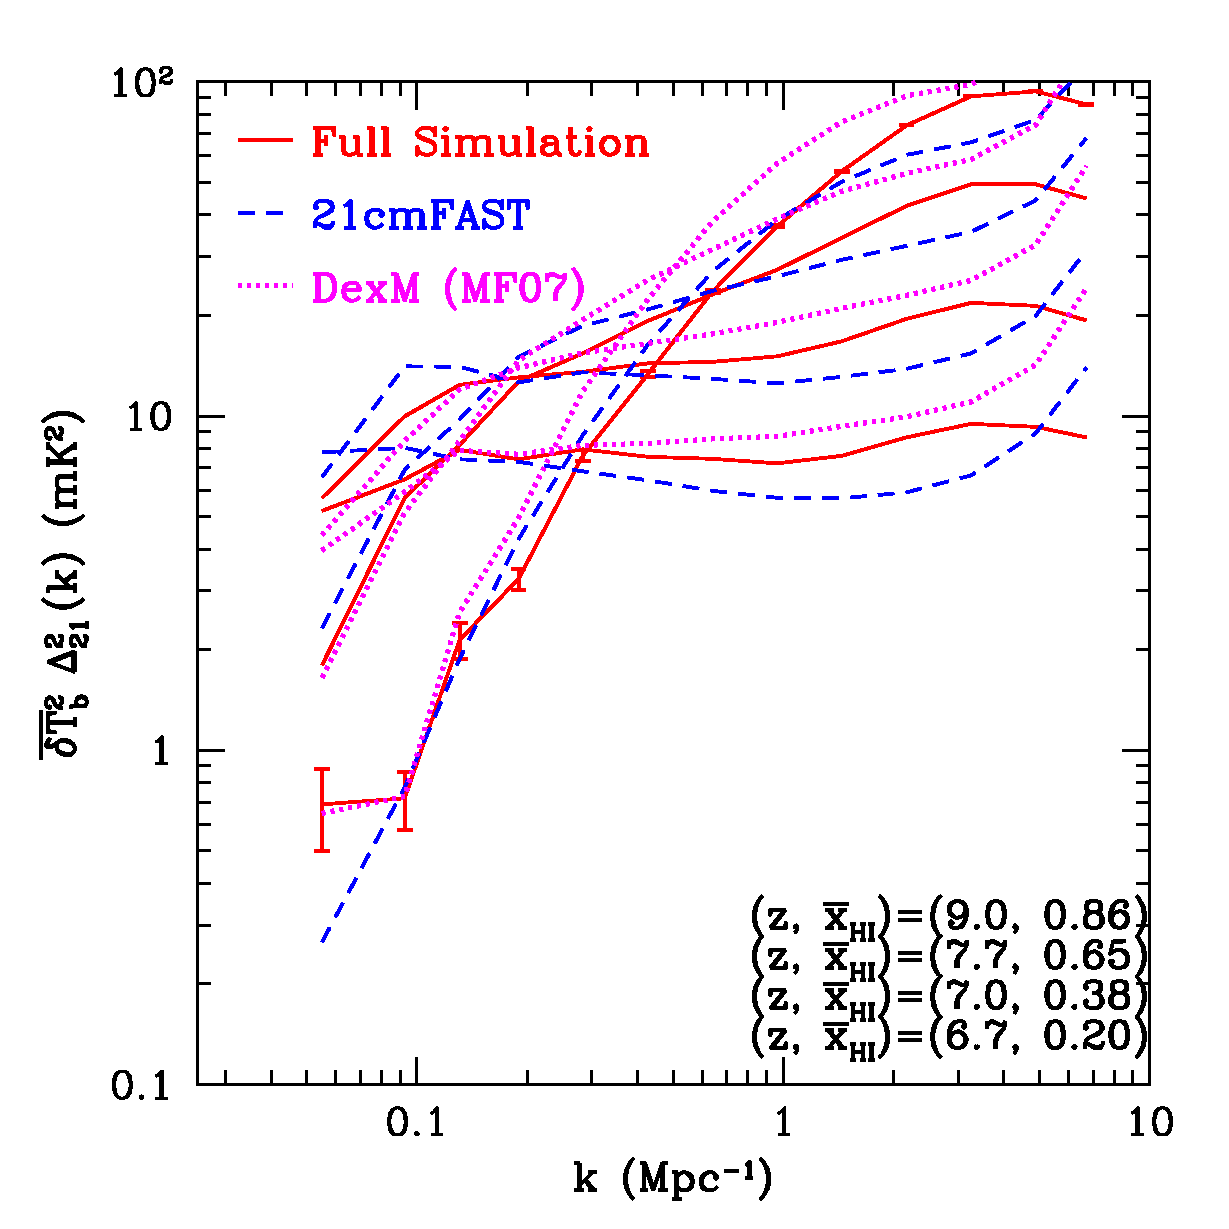
\includegraphics[width=0.6\linewidth]{EoR/c03/c03.s3.f1.eps}
\centering
\caption{$B%7%_%e%l!<%7%g%s7k2L!J@V@~!K!"(B21cmFAST$B$N7k2L!J@D?'!K!"(BDeXM(21cmFAST$B$NA0?H(B)$B$N7k2L!J%^%<%s%?!K(B}
\label{fig:ps}
\end{figure}
$B0J>e$,(B21cmFAST$B$G9T$o$l$k7W;;$N35N,$G$"$k!#(B
%既存の計算手法(21cmFASTを例にして)
\input{EoR/c03/c03.s3.ss2.tex}%問題点
\subsection{SKA-JP $B:FEEN%HI$N@oN,(B}
%\label{EoR.s4}
\label{c03.s3.ss3}
\subsubsection{(1)$BF|K\HG(B21 cmFAST$B%3!<%I$N9=C[(B}
$B4QB,%G!<%?$+$i=iBeE7BN!&6d2O$N7A@.$K4X$9$k>pJs$rF@$k$?$a$K$O!"Hf3S$KBQ$((B
$B$k@:EY$r$b$DM}O@%b%G%k$N9=C[$,IT2D7g$G$"$k!#FC$KCf@-?eAG$+$i$N%7%0%J%k$r(B
$B?dDj$9$k$K$O!"0E9uJ*<A$H%,%9$N=ENOIT0BDj@-$K$h$k@.D9$K2C$(!"=iBeE7BN!&6d(B
$B2O$N7A@.$H$=$3$+$iJ|$?$l$k(BX$B@~!&;g30@~$K$h$k%,%9$N2CG.!&:FEEN%$r7W;;$7$J$1(B
$B$l$P$J$i$J$$!#(B

SKA$B$K$h$C$F:FEEN%4|$K$*$1$kCf@-?eAG(B21 cm$B@~$,4QB,$G$-$l$P!":FEEN%$N;~4|!"(B
$BH/E8$N;EJ}!"EEN%8w;R8;$J$I$3$l$^$GL$2rL@$G$"$C$?>pJs$rF@$k;v$,$G$-$k!#$^(B
$B$?!":FEEN%4|$O!"B>GHD9$N<!@$Be4QB,5!4o$N%?!<%2%C%H$H$J$C$F$$$k;~4|$G$"$j!"(B
$BB>GHD9$N4QB,7k2L$+$i$/$k@)8B$rMQ$$$l$P!":FEEN%$K4X$9$kM}2r$OHtLvE*$K?J$`(B
$B$H4|BT$G$-$k!#$7$+$7!"(B\ref{c03.s3.ss1}$B$d9q:]%5%$%(%s%9%V%C%/$N>R2p$NItJ,(B
$B$G$b$"$k$h$&$K!"$3$l$^$G$N8&5f$O!"J|<M8;E7BN$d6d2O4VJ*<A$N%b%G%j%s%0$K4X(B
$B$7$FITDj@-$,Bg$-$/!"8=>u$N$^$^$G$O>\:Y$JM}O@M=B,$O:$Fq$G$"$k!#(B

$B$3$N@a$G$O!"9q:]%5%$%(%s%9%V%C%/>R2p$N>O$G$9$G$K?($l$?@$3&$G9T$o$l$F$$$k(B
$B:FEEN%$N7W;;<jK!(B(\ref{c03.s2.ss2})$B$r$b$&0lEY4JC1$K>R2p$7!"$=$N8e(B SKA-JP$BFH(B
$B<+$N%"%W%m!<%A$*$h$S$=$l$K$h$C$F2~A1$5$l$kE@$r5-$9!#(B

\medskip 

$B$3$l$^$G!"1'Ch:FEEN%$NM}O@E*8&5f$O<g$K=`2r@O!&=`?tCME*7W;;!"$*$h$S?tCM%7(B
$B%_%e%l!<%7%g%s$K$h$C$F9T$o$l$F$-$?!#(B1-zone$B$N=`2r@OE*<jK!$G$O!"(B
Press-Schechter formalism$BEy$rMQ$$$F3F@VJ}JP0\$4$H$N(BDM$B%O%m!<<ANL4X?t$rF3=P(B
$B$7!"$=$3$KMM!9$J(BBaryonic Physics$B$r2>Dj$9$k;v$G!"1'Ch$NJ?6QE*$JG.!&EEN%?J(B
$B2=;K$r7W;;$9$k!#$3$N<jK!$O!">/$J$$7W;;NL$G1'Ch$NBg6IE*$J?J2=$rD4$Y$k;v$O(B
$B$G$-$k$,!"(B21 cm$B$N%Q%o!<%9%Z%/%H%k$J$I$N6u4VE*>pJs$,I,MW$H$J$kNL$OM=B,$G$-(B
$B$J$$!#$3$l$r2~NI$7$?$N$,!"(B21cmFAST$BEy$rMQ$$$?!"=`?tCME*$J%"%W%m!<%A$G$"$k!#(B
$B$3$N%"%W%m!<%A$O!"Hf3SE*0B2A$J7W;;%3%9%H$GEEN%9=B$$r7W;;$9$k;v$,2DG=$G$"(B
$B$j!"(BSKA$B$K$h$k4QB,$H$ND>@\E*Hf3S$,2DG=$H$J$k$h$&$J?t(B100Mpc-1Gpc
(comoving)$B$N7W;;NN0h$r$H$k;v$b2DG=$G$"$k!#$^$?!"7W;;%3%9%H$N>/$J$5$+$iBg(B
$B$-$J%Q%i%a!<%?6u4V$r$H$l$kEy$NMxE@$,$"$k!#$7$+$7!"MM!9$JLdBj$b$"$k(B
(\ref{c03.s3.ss1})$B!#(B

$B0lJ}$G!"?tCM%7%_%e%l!<%7%g%s$K$h$k%"%W%m!<%A$G$O!"EEN%8w;R$NM"Aw2aDx$r2r(B
$B$/;v$G6d2O4V6u4V$NCf@-?eAGJ,I[$r5a$a$k!#$3$NmU<MM"Aw7W;;$O!"=`?tCME*%"%W(B
$B%m!<%A$KHf$Y$F9b$$7W;;%3%9%H$,MW5a$5$l$k$,!"Hs0lMML)EY>l$G$NCf@-?eAGJ,I[!&(B
$B29EYJ,I[$r@:EY$h$/5a$a$k;v$,$G$-$k$H$$$&MxE@$,$"$k!#$3$N$h$&$J7W;;$O!"(B
2000$BG/Be$KF~$j7W;;5!@-G=$N8~>e!"7W;;%"%k%4%j%:%`$NH/C#$K$h$j2DG=$H$J$j!"(B
$B1'ChO@E*N.BN!&(B$N$$BBN7W;;$K$h$C$FJ*<AJ,I[$r7W;;$7$?8e$K%]%9%H=hM}$K$h$C$FCf(B
$B@-?eAGJ,I[!&29EYJ,I[$r7W;;$9$k$N$,8=:_$N<gN.$H$J$C$F$$$k!#(B

$B0J>e$,@$3&E*$K9T$o$l$F$-$?:FEEN%8&5f$N<g$J%"%W%m!<%A$G$"$k$,!"$3$N$h$&$J(B
$B%"%W%m!<%A$G$O!"EEN%9V8w;R8;$H$J$k6d2O%b%G%k$*$h$S6u4VE*$KJ,2r$G$-$F$$$J(B
$B$$6d2O4VJ*<AHs0lMM@-$N%b%G%k$NITDj@-$,Bg$-$$!#$3$l$i$O!":FEEN%4|$NCf@-?e(B
$BAGJ,I[$N7hDj$K;YG[E*$JMWAG$G$"$k$,!"(BX$B@~!&;g30@~$K$h$k1F6A$r<u$1!"Hs>o$KJ#(B
$B;($J?J2=$r<($9;v$,4|BT$5$l$k!#$3$l$i$r7W;;$9$k$?$a$K$O!"mU<MM"Aw$H$=$N1F(B
$B6A2<$G$NN.BN$N?6$kIq$$$rL7=b$J$/2r$-$"$2$k1'ChO@E*mU<MN.BNNO3X7W;;$,I,MW(B
$B$H$J$k!#$3$N$h$&$JmU<MN.BN7W;;$O!"Hs>o$KKDBg$J7W;;%3%9%H$N0YD9$i$/<B8=$,(B
$B:$Fq$G$"$C$?$,!"(B2010$BG/0J9_=y!9$KA}$($D$D$"$k!#$7$+$7!"@$3&E*$K$b<B8=Nc$O(B
$B$^$@>/?t$G$"$j!"7W;;NN0h$b?t(BMpc-$B?t(B10Mpc (comoving)$B$H(BSKA$B4QB,$H$ND>@\Hf3S$K(B
$B$O>.$5$9$.$k$N$,8=>u$G$"$j!"?t(B100Mpc$B0J>e$N%9%1!<%k$G$NmU<MN.BN7W;;$N<B8=(B
$B$OHs>o$K:$Fq$G$"$k!#$3$N0Y!"4{B8$N%b%G%k$NITDj@-$r4KOB$9$k8=<BE*$J2r7h:v(B
$B$O!"mU<MN.BNNO3X7W;;$K$h$k7k2L$r%b%G%k2=$7$F!"Bg5,LO$N=`?tCME*<jK!Ey$KAH(B
$B$_9~$`;v$G$"$m$&!#(B

SKA-JP$B$O!"@$3&$K@h6n$1$F1'ChO@E*mU<MN.BN7W;;$r<B9T$7$?7P83$r6/$_$H$7(B 
\citep{2013MNRAS.428..154H}$B!"$3$l$rMxMQ$7$?%5%$%(%s%9$r9T$&!#2f!9$O!"mU(B
$B<MN.BNNO3X$K$h$k7k2L$r2r@O$7$F?.Mj@-$N9b$$%b%G%k$r:n@.$7!"$3$l$rAH$_9~$`(B
$B$3$H$G!"$h$j9bB.$+$D@53N$K1'ChO@E*Bg%9%1!<%k$G$N:FEEN%4|$N(B21 cm$B%7%0%J%kM=(B
$BB,$7$&$k?7$?$J=`?tCME*%7%_%e%l!<%7%g%s%3!<%I$r3+H/$r9T$&!#6qBNE*$K$O0J2<(B
$B$N$h$&$J2~NI$r;\$9!#(B

%$B:G=*E*$J%3!<%I$NL\I87W;;;~4V$O(B?\\
%$B8=>u$N$^$^$G$b!"?tCM%7%_%e%l!<%7%g%s$KHf$Y$l$PHs>o$K9bB.$G$"$k$7!"(B
%$B<+A0(BPC$B$G$b7W;;2DG=$JHO0O$G$"$k!#$I$N$h$&$J;H$$J}$rA[Dj$7$F!"$I$N(B
%$B$/$i$$$N7W;;;~4V$r5a$a$k$+!)(B

\begin{itemize}
 \item $B=iBe@1=i4|<ANL4X?t$N%b%G%k2=(B
 
 	$B1'Ch:FEEN%$O!"1'Ch$G:G=i$K7A@.$5$l$k@1$N=iBe@1$+$i$N;g30@~(B
	$B$K$h$C$F;O$^$k$H4|BT$5$l$k$,!"=iBe@1$,$I$NDxEY:FEEN%$K4sM?(B
	$B$9$k$+$O!"=iBe@1$N<ANL!&7A@.N($K0MB8$9$k!#(B
	$B=iBe@1$N1'ChO@E*7A@.N($O!"=iBe@17A@.$K$h$C$F5^B.$KH/C#$9$k(B
	$B?eAGJ,;R2rN%mU<M>l$N6/EY$K0MB8$9$k!#$3$N:]!"=iBe@1$+$iJ|<M(B
	$B$5$l$kEEN%8w;R$H2rN%8w;R$NHf$O=iBe@1$N<ANL$K0MB8$9$k0Y!"@5(B
	$B3N$JEEN%?J2=$N7W;;$K$O!"=iBe@1<ANL4X?t$N>pJs$,I,?\$H$J$k!#(B
	$B=iBe@1$N<ANL4X?t$K4X$9$kM}O@E*8&5f$G$OF|K\$,@$3&$r%j!<%I$7(B
	$B$F$*$j(B \citep{2014ApJ...781...60H, 2014ApJ...792...32S}$B!"(B
	$B$3$l$rMQ$$$k;v$GF|K\$NM}O@8&5f$NFC?'$,=P$;$k!#(B
 \item $BmU<MN.BN7W;;7k2L$N2r@O$K$h$k%5%V%0%j%C%I%b%G%k$N:n@.(B

 	{\bf $B;g30@~8w;R$NC&=P3d9g$N4D6-!&;~9o0MB8@-$NF3F~(B}$B!':FEEN%4|$N<g(B
	$B$?$kEEN%8w;R8;$H$7$F4|BT$5$l$k6d2O$+$i$NEEN%8w;R6!5kNL$O!"(B
	$B6d2OFb$NEEN%8w;R@8@.N($*$h$S@8@.$5$l$?EEN%8w;R$NC&=P3d9g$K(B
	$B$h$C$F7hDj$5$l$k!#(B
	$B:FEEN%4|$NEEN%NN0h$N%5%$%:J,I[$O!"EEN%8w;R8;$N6u4VJ,I[(B($B%/%i%9%?%j%s%0(B)
	$B$*$h$S$=$l$>$l$N8w;R8;$+$i6d2O4V6u4V$X$NEEN%8w;R6!5kNL$,=EMW$J$k0Y!"(B
	$B:FEEN%4|$NCf@-?eAG(B21 cm$B%7%0%J%k$N@53N$JM=B,$K$O!"6d2O$N>\:Y(B
	$B$J%b%G%j%s%0$,I,?\$H$J$k!#(B
	$BEEN%8w;R@8@.N(!&EEN%8w;RC&=P3d9g$O!"@1$+$i$N;g30@~$dD6?7@1(B
	$BGzH/$K$h$k%U%#!<%I%P%C%/!"%@%9%H$K$h$kJ,;R7A@.B%?J!&;g30@~(B
	$B5[<}!"1'ChO@E*$J%O%m!<$X$N%,%99_Ce;K$d;g30@~GX7JJ|<M$N6/EY(B
	$B$J$I$N$NMm$_$"$C$?Hs>o$KJ#;($J2aDx$K0MB8$9$k!#(B
	$B:#2s$N%"%W%m!<%A$G$O9bJ,2rG=$NmU<MN.BN7W;;$K$h$C$F6d2O$N(B
	$BEEN%8w;R@8@.N(!&EEN%8w;RC&=P3d9g$N%O%m!<<ANL!";~9o!"4D6-(B
	$B0MB8@-$rL@$i$+$K$7!"$3$l$r%F!<%V%k2=$"$k$$$O4X?t2=$7$F=`?t(B
	$BCME*<jK!$KAH$_9~$`!#(B

       \medskip

	{\bf $B6d2O4VJ*<A$NHs0lMM@-$N4D6-!&;~9o0MB8@-$NF3F~(B}$B!'6d2O4VJ*<ACf(B
       $B$G$NEEN%?J2=$O!"$=$N>l=j$G$N:F7k9gN($K0MB8$9$k!#:F7k9gN($OL)EY$N(B
       $B<+>h$KHfNc$9$k0Y!"EEN%%,%9$N%/%i%s%T%s%0%U%!%/%?!<!"(B$C_{\rm
       H\textsc{ii}}\equiv \langle n_{\rm H\textsc{ii}}^2\rangle / \langle n_{\rm
       H\textsc{ii}}\rangle^2$$B$,=EMW$H$J$k!#DL>o$N=`?tCME*7W;;$d%]%9%H=hM}E*$JmU(B
       $B<MM"Aw%7%_%e%l!<%7%g%s$G$O!">.%9%1!<%k$N6d2O4VJ*<A$,J,2r$G$-$F$$(B
       $B$J$$>e!"8w2CG.$K$h$C$F(B$C_{\rm H\textsc{ii}}$$B$,>.$5$/$J$k8z2L(B (e.g.,
       \cite{2009MNRAS.394.1812P}) $B$,9MN8$G$-$F$$$J$$!#%5%V%0(B
	$B%j%C%I%b%G%k$H$7$F(B$C_{\rm H\textsc{ii}}$$B$rMQ$$$k;v$G:F7k9gN($KJd@5$r(B
	$BF~$l$k>l9g$b$"$k$,!"(B$C_{\rm H\textsc{ii}}$$B$N6u4VE*Hs0lMM@-$,9MN8$5$l(B
	$B$F$*$i$:F@$i$l$kEEN%9=B$$,@53N$G$O$J$$!#:#2s$N2f!9$N%"%W%m(B
	$B!<%A$G$O9bJ,2rG=$NmU<MN.BN7W;;7k2L$+$i!"L)EY$HEEN%EY$N4X(B
	$B?t$H$7$F(B$C_{\rm H\textsc{ii}}$$B$r%F!<%V%k2=$b$7$/$O4X?t2=$7$FMQ$$$k;v(B
	$B$G!";g30@~$K$h$k%U%#!<%I%P%C%/$*$h$S6u4VE*Hs0lMM@-$r9MN8$7(B
	$B$?(B$C_{\rm H\textsc{ii}}$$B$rA[Dj$G$-$k!#(B


 \item $N$$BBN7W;;!"$^$?$O9b<!@]F07W;;$K$h$k=ENO>l$N@:L)2=(B

 	$BDL>o$N=`?tCME*<jK!$GMQ$$$i$l$k%<%k%I%S%C%A6a;w$G$O!">.%9%1(B
	$B!<%k9=B$$G$N@:EY$,ITB-$9$k!#$^$?!"DL>o?t(B100kpc$B$N6u4VJ,2rG=(B
	$B$G$N7W;;$G$"$k$?$a!"3F>l=j$K4^$^$l$k%O%m!<$N8D?t!&<ANL4X?t(B
	$B$N>pJs$,7gMn$9$k!#(B\ref{c03.s2.ss2}$B@a$G$b?($l$?$h$&$K!"%O%m!<>pJs(B
	$B$N7gMn$O!":FEEN%;K$N7W;;$KBg$-$J8m:9$rM?$($k!#(B
	$B$3$l$i$NLdBj$r2sHr$9$k$?$a!"8=>u(B2$B$D$N0F$HA[Dj$7$F$$$k!#(B
	$B$R$H$D$O$h$j9b<!$N@]F0O@$rMQ$$$FL)EY>l@8@.$r9T$&J}K!$G$"$k!#(B
	$B$3$N>l9g!">.%9%1!<%k$G$N%:%l$O4KOB$5$l$k$H;W$o$l$k$,!"4D6-(B
	$B$4$H$N%O%m!<>pJs$O7gMn$7$?$^$^$G$"$k$?$a!"6I=jE*$JL)EY(B
	$B$N4X?t$H$7$F%O%m!<$N<ANL4X?t$*$h$S>e5-$N6d2O%b%G%k$rAH$_9~$`!#(B
	$B$b$&0l$D$N%"%W%m!<%A$O!"(B$N$$BBN7W;;$r0lEY$7$F$*$-!"3F;~4|$K$*$1(B
	$B$k%O%m!<J,I[!"L)EYJ,I[$rJ]B8$7$F$*$/<jK!$G$"$k!#$3$N>l9g!"(B
	$B=`?tCME*7W;;$r9T$&$?$S$K(B$N$$BBN7W;;$r$9$kI,MW$3$=$J$$$,!"7W;;NN(B
	$B0h$r9-$2$?7W;;$r9T$&>l9g!"Bg5,LO$J(B$N$$BBN7W;;$,I,MW$H$J$k!#(B

 \item relative velocity effect ($B=i4|1'Ch$G$N2;6A?6F0$K$h$j%@!<%/%^%?!<(B
       $B$HDL>oJ*<A$NB.EY>l$N$:$l(B)$B$K$h$k%O%m!<7A@.$NM^@)8z2L$rF3F~(B

       \cite{2010PhRvD..82h3520T}$B$K$h$C$F;XE&$5$l$?!"(Brelative velocity
       effect $B$O>.%9%1!<%k$NL)EYMI$i$.$N>e!"@2$l>e$,$j0JA0$NBg%9%1!<%k$N(B
       $B2;6A?6F0$K$h$k%P%j%*%sN.$,>h$k$H$$$&>u67$G$"$k!#E}7WE*$J4QB,NL$K(B
       $BBP$9$k1F6A$N$_$KCeL\$9$k>l9g$K$O!"(Brelative velocity effect $B$K$h$k(B
       $B9=B$7A@.$NM^@)$N8z2L$NBg$-$5$r5eBP>NJx2u%b%G%k$r3HD%$9$k$3$H$K$h(B
       $B$j8+@Q$j!"(BPress-Schechter$B7?$NM}O@$K<h$jF~$l$k$3$H$K$h$jI=8=$9$k$3(B
       $B$H$,$G$-$k$O$:$G$"$k!#(B\footnote{$BDc<ANL%O%m!<7A@.$X$N1F6A$O$3$l$^(B
       $B$G8&5f$,$J$5$l$F$-$?$,!"%U%#%i%a%s%H$d$h$jDcL)(B $BEY$N>l=j$K$*$1$k1F6A(B(IGM
       clumping factor $B$X$N1F6A!"%,%929EY$X$N1F6A(B)$B$O$J$$$+(B?$B$K$D$$$F$bD4(B
       $B$Y$kI,MW$,$"$k(B($BD9C+@n(B)$B!#(B}$B@53N$K$H$j$3$`$?$a$K$O!"Bg%9%1!<%k$N%7(B
       $B%_%e%l!<%7%g%s%\%C%/%9$rMQ0U$7$?Cf$G%@!<%/%^%?!<$H%P%j%*%s$NFsN.(B
       $BBN7W;;$r!"(B($B%@!<%/%^%?!<$H%P%j%*%s$N1?F0$N$:$l$r9MN8$7$?(B)$BE,@Z$J=i(B
       $B4|>r7o$N$b$H$G2r$/I,MW$,$"$k!#$3$N7W;;$r<B9T$7!"1F6A$NBg$-$5$r8+(B
       $B@Q$b$k!#8=:_L>8E20Bg3X$N^I1);a$rCf?4$K6a;wE*5eBP>NJx2uLO7?$rMQ$$(B
       $B$FH>2r@OE*$J%b%G%j%s%0$X8~$1$?8&5f$,?J$s$G$$$k!#(B
\end{itemize}


\paragraph{(2)$BDc<~GHNN0h$NA07JJ|<M$N%b%G%k2=$H=|5nJ}K!$N9=C[(B}

$B1'Ch:FEEN%4|$+$i$N%7%0%J%k$KBP$7!"7OFb!&30$+$i$NEEGHJ|<M$,6/Nu$JA07J$H$J(B
$B$k$?$a!"$3$l$r<h$j=|$/I,MW$,@8$8$k!#;d$?$A$O0l:rG/$+$i!":FEEN%4|$N4QB,Au(B
$BCV$H$7$F:G9b@-G=$r$b$D%*%i%s%@(BLow Frequency Array (LOFAR) $B%0%k!<%W$H$N6&(B
$BF18&5f$r;O$a$F$*$j!"(BAGN$B$J$I$N%3%s%Q%/%HEEGH8;!"$*$h$S7OFb$N%7%s%/%m%H%m%s(B
$BJ|<M$,LdBj$H$J$k$3$H$rL@$i$+$K$7$F$$$k!J(BKumazaki et al., submitted$B!K!#$H(B
$B$/$K!"$3$l$iA07JJ|<M$,:FEEN%4|(B $B$N%7%0%J%k$KBP$7$F$I$NDxEY%N%$%:$H$J$k$+$K(B
$B$D$$$F!"%7%_%e%l!<%7%g%s$K$h$kI>2A8&5f$r9T$C$F$-$?<B@S$,$"$k!#L>8E20Bg3X(B
$B$G$O$3$l$^$GF|K\3X=Q?66=2qJd=u6b!VF,G>=[4D$r2CB.$9$k<c<j8&5f<T@oN,E*3$30(B
$BGI8/%W%m%0%i%`!W7PHq$K$h$j!"<c<j(B3$BL>$r%*%i%s%@(BLOFAR$B%0%k!<%W$XGI8/$7!"6&F1(B
$B8&5f$r?J$a$F$-$?!#$=$3$G!"$3$N?M:`8rN.$N<B@S$r3hMQ$7!"(BLOFAR$B$N4QB,%G!<%?$r(B
$BMQ$$$?4QB,E*$J8&5f$r9T$&!#<B:]$N%G!<%?$rMQ$$$k$3$H$GDc<~GHEEGH2r@O$N5;=Q(B
$B$r<hF@$9$k$H$H$b$K!":GBg8B$N>pJs$r%G!<%?$+$iF@$k$?$a$NI,MW$J=hM}!"$H$/$K(B
$BA07JJ|<M$N:9$70z$-$K$D$$$F!"M}O@E*$J8&5f$r?J$a$k!#$3$N%b%G%k2=$K$O!"6d2O(B
$B7O$r0l$D$N6d2O$H$H$i$($kN)>l$+$i6d2O?J2=$NCN8+$,D>@\1~MQ$G$-$k$@$m$&!#(B

$B$3$3$G$OFC$K!"$3$l$^$G%7%_%e%l!<%7%g%s$rMQ$$$?8&5f$K$*$$$FE,@Z$JI>2A$,$J(B
$B$5$l$F$$$J$+$C$?!"CO5eEEN%AX$N8z2L$r9MN8$7$?$h$j8=<BE*$JA07JJ|<M%b%G%k$r(B
$B9=C[$9$k!#!!$3$N%b%G%k$KBP$7!"MM!9$J<jK!$K$h$kA07JJ|<M=|5nK!$rE,MQ$7$=$N(B
$B@-G=$rE0DlE*$KHf3S$7$D$D!"9b@VJ}JP0\$7$?(B21 cm$B@~4QB,$KFC2=$7$?A07JJ|<M=|5n(B
$BK!$r3+H/$9$k!#$3$l$^$G$K(BCMB$B$NA07JJ|<M$K$D$$$F$N8&5f(B
\citep{2014ApJ...780...13I}$B!"@V30@~GX7JmU<M$K$D$$$F$N8&5f(B
\citep{2001PASJ...53...37T,2001PASP..113..586T,2004ApJ...604...40T,2011ApJ...737....2M}
$B<B@S$,$"$k$N$G!"$3$l$i$N8&5f$r1~MQ$9$k!#(B 

%SKA-JP 再電離班の戦略


\input{EoR/EoR.bib.tex}
\input{EoR/EoR.author.tex}


\chapter{宇宙論}\label{cosmology}

\section{イントロダクション:標準宇宙論と未解決問題}\label{cosmology.s1}

\subsection{宇宙論の現状}\label{cosmology.s1.ss1}

%%%%%%%%%Figure%%%%%%%%%%%%%%%%%%%%%%%%%%%%%%%%%%%%%%%%%%%%%%%%%%%%%%%%%%%%%
\begin{figure}[t]
\begin{center}
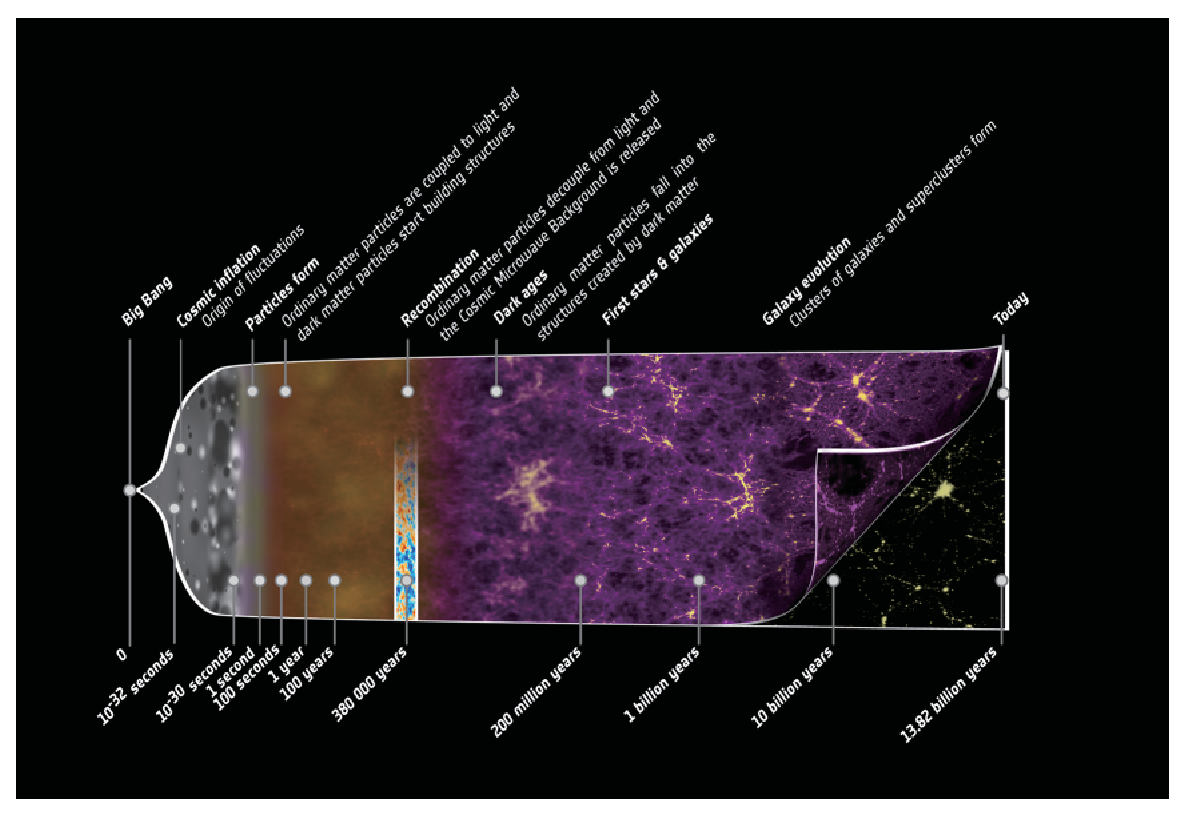
\includegraphics[width=0.8\linewidth]{cosmology/Planck_history_of_Universe_Crop_orig.eps} 
\caption{宇宙の構造進化の歴史(Planck web pageより)。}\label{fig:cosmo_history}
\end{center}
%\end{figure}
%%%%%%%%%%%%%%%%%%%%%%%%%%%%%%%%%%%%%%%%%%%%%%%%%%%%%%%%%%%%%%%%%%%%%%%%%%%%

%%%%%%%%%Figure%%%%%%%%%%%%%%%%%%%%%%%%%%%%%%%%%%%%%%%%%%%%%%%%%%%%%%%%%%%%%
%\begin{figure}[t]
 \begin{minipage}{0.6\hsize}
 \begin{center}
   \vspace{15pt}
   \includegraphics[width=0.7\linewidth]{cosmology/Planck_CMB_Mollweide_4k_2.eps} 
   \vspace{10pt}
   \caption{PlanckによるCMB温度揺らぎの全天マップ(Planck web pageより)}\label{fig:Planck_CMB}
 \end{center}
 \end{minipage}
 \begin{minipage}{0.4\hsize}
 \begin{center}
   \includegraphics[width=0.8\linewidth]{cosmology/component_univ.eps} 
  \vspace{-15pt}
  \caption{宇宙の構成成分(Planck web pageより)。}\label{fig:component}  
 \end{center}
 \end{minipage}
\end{figure}
%%%%%%%%%%%%%%%%%%%%%%%%%%%%%%%%%%%%%%%%%%%%%%%%%%%%%%%%%%%%%%%%%%%%%%%%%%%%

宇宙論とは、宇宙全体やその内部に存在する構造物が、どのように形成されそして発展してきたのかについて、科学的手法を用いて理論的・観測的に解明していく学問である(図~\ref{fig:cosmo_history})。特に近年の観測技術の発達により、標準的な宇宙モデルはほぼ確立しており、それは次のようなものである。

まず、大局的なスケール(超銀河団を超えるスケール、約$100$Mpc以上)で宇宙を平均して見た場合、特別な場所は存在せず(一様性)、また特別な方向も存在しない(等方性)という一様等方宇宙モデルを採用している。現在のところ、このモデルが成り立っていないという確実な証拠は存在しない。さらに、宇宙内部の構成物についても、ビッグバン後約$38$万年頃に原子が形成され光が直進できるようになった時期の残光である宇宙マイクロ波背景放射(Cosmic Microwave Background radiation : CMB)の精密観測が行われたことにより(図\ref{fig:Planck_CMB})、このモデルの妥当性が確認されている。最新のCMB観測衛星Planck~\citep{Ade:2013zuv}の観測結果によると、通常の物質を構成するバリオンの量は、宇宙全体の約$5$\%程度に過ぎず、約$27$\%がほぼ重力相互作用しか行わない冷たい暗黒物質(cold dark matter)で構成され、さらに約$68$\% が宇宙の膨張を加速させる原因となる正体不明のエネルギー(暗黒エネルギー:dark energy)であるということが分かっている(図~\ref{fig:component})。またこのモデルでは一定の空間曲率が許されているが、CMBの観測からこの曲率は非常に小さく制限されており、この宇宙は平坦な宇宙であるということが判明している。典型的な宇宙論パラメータを表\ref{cosmological parameters1}, \ref{cosmological parameters2}に示す。

このように一様等方宇宙モデルは、観測を非常に良く説明するモデルであるが、そもそもなぜこのような条件の宇宙が生じたのかという疑問が生じてくる。その疑問に対し説明を与える最も有力なモデルが、宇宙初期における指数関数的急膨張(インフレーション)を仮定するモデルである。このインフレーションモデルでは、宇宙初期の光速を超える急膨張によって、当初因果関係を持っていた小さな領域を現在観測可能な範囲(宇宙の地平線)を超えて拡大することにより、非常に一様で等方な宇宙を実現することができる。またこの膨張によって、曲率は均されて小さくなり、非常に平坦な宇宙が実現する。さらにインフレーションモデルでは、インフレーションを生じさせる場としてインフラトンという場を仮定するが、その場の量子的な揺らぎから、銀河などの大規模構造の種となるわずかな密度揺らぎを生成することも可能にしている。

以上が現在標準的な宇宙モデルであるが、その上で今後解明を目指すべき重要な問題としては、次のようなものを挙げることができる:
(i) インフレーションモデルの検証、
(ii) 暗黒エネルギーの性質の解明及び修正重力理論の可能性の検証、
(iii) 暗黒物質の正体の特定。
以下で、これらの問題についての解説及びその観測的な制限について順に説明していく。

%\vspace{10pt}


%TTTTTTTTTTTTTTTTTTTTTTTTTTTTTTTTTTTTTTTTTTTTTTTTTTTTTTTTTTTTTTTTTTTTTTTTT%
\begin{center}
\begin{table}[t]
\caption{
標準的な宇宙論($\Lambda$CDM模型)におけるパラメータおよび$68\%$ C.L.エラー~\citep{Ade:2013zuv}。
}
\begin{center}
 \vspace{15pt}
\begin{tabular}{ccc} \hline \hline 
宇宙論パラメータ & 値 & 定義 \\ 
\hline 
$\Omega_{\rm b}h^2$ & $0.02214\pm 0.00024$ & 現在のバリオン密度\\
$\Omega_{\rm c}h^2$& $0.1187\pm 0.0017$ & 現在の冷たい暗黒物質密度\\
$\tau$ & $0.092\pm 0.013$ & 再電離によるトムソン散乱の光学的厚さ\\
$\ln (10^9 A_{\rm s})$ & $3.091\pm 0.025$ & 原始曲率揺らぎパワースペクトルの振幅\\
$n_{\rm s}$ & $0.9608\pm 0.0054$ & 原始曲率揺らぎパワースペクトルの冪指数\\
%\hline
$H_0=100h$ & $67.80\pm 0.77$ & 現在のハッブル定数 $[{\rm km}/{\rm s}/{\rm Mpc}]$\\
$\Omega_\Lambda$ & $0.692\pm 0.010$ & 現在の暗黒エネルギー密度\\
\hline
\hline 
\end{tabular}
\end{center}
\label{cosmological parameters1}
\end{table} 
\end{center}
%TTTTTTTTTTTTTTTTTTTTTTTTTTTTTTTTTTTTTTTTTTTTTTTTTTTTTTTTTTTTTTTTTTTTTTTTT%


%%%%%%%インフレーション関係%%%%%%%%%%%%%%%%%%%%%%%%%%%%%%%%%%%%%%%%%%%%%%%%%
\paragraph{(i) インフレーションモデルの検証}
%まず始めに、インフレーションモデルの検証方法について説明していく。
%
インフレーションモデルの検証において最も基本的な方法は、宇宙の密度揺らぎの測定である。これまで述べたように、インフラトンの量子揺らぎは最終的に密度揺らぎの起源となるが、この揺らぎはインフレーションのモデルの違いによって、特徴のある空間スケール依存性を示す。よって、その特徴を観測的に捉えることが、各インフレーションモデルを制限していく上で非常に有効な手段となる。

またインフレーションで生成される密度揺らぎはほぼガウス分布に従うことが知られているが、各モデルによってガウス分布からの微小なズレの程度(原始非ガウス性)が異なっている。そのため、この原始非ガウス性を測定することもこのモデルを制限する非常に有効な方法の一つである。
インフレーションの一般的なモデルでは、確率分布として様々な非ガウス性を持つ原始揺らぎを生成しうる。
原始揺らぎのガウス分布からのズレを表す最も便利な方法として、重力ポテンシャル$\Phi$が
ランダムガウス場$\phi$の線形項と2次の補正の和で
\begin{align}
	\Phi =\phi +f_{\rm NL}\left(\phi^2 -\langle\phi^2\rangle\right)
	\,.\label{eq:fNL def}
\end{align}
と書かれる場合を考える。
ここで、$f_{\rm NL}$は非線形パラメータと呼ばれる定数であり、$\langle\cdots\rangle$はアンサンブル平均を表す。
この場合、その統計的性質はパワースペクトルだけでは記述できず、
バイスペクトルのような高次のモーメントが必要になる。
異なるインフレーション模型は異なるバイスペクトルの形を予言することから、この探求により
インフレーションの物理について深い理解を得ることができる。
これまでCMBの精密な観測により、インフレーションの物理に対して精度よく制限がなされている(\ref{cosmology.s1.ss2}節)。
特に、Planck衛星による観測~\citep{Ade:2013ydc}によれば、非線形パラメータは$f_{\rm NL}=2.7\pm 5.8$となる制限が得られており、$f_{\rm NL}>10$となるような比較的大きな非ガウス性を生成するモデルや、モデル内のパラメータを制限することに成功している。
後述するように、銀河サーベイからも原始非ガウス性を探査することができる。
しかし、未知の系統誤差の影響により、現在までの制限は$\sigma (f_{\rm NL})\approx 50$程度に留まっている\citep{Ho:2013lda,Giannantonio:2013uqa}。

加えて、インフレーションの検証に非常に重要な観測として、インフレーション起源の原始重力波の観測が挙げられる。この原始重力波は、インフレーション中に重力場の量子揺らぎから生成されたものであり、その振幅はインフレーションのエネルギースケールと直接関係づくことが知られている。そのため、もしこの原始重力波を観測できれば、地上の加速器実験ではとても到達できない、
%ほど大きなエネルギーのスケールである
インフレーションの生じた超高エネルギーの物理の情報を直接知ることができるのである。

%現在、Planck衛星によるCMB温度揺らぎの観測から揺らぎのスケール依存性や原始重力波の強い制限が得られており~\citep{Ade:2013uln}、今後はより精密なCMB偏光の観測や、広い範囲の銀河サーベイ、または再電離の時期の水素が発する21cm線の観測によって、更に高い精度でインフレーションモデルの検証が行えると期待される。
%制限が得られると期待されている。
%また
%原始重力波については、
%その原始重力波の振幅が比較的大きなものであれば、
%将来の宇宙重力波干渉計を用いれば、原始重力波のスペクトルを直接観測できる可能性さえ存在している。


%TTTTTTTTTTTTTTTTTTTTTTTTTTTTTTTTTTTTTTTTTTTTTTTTTTTTTTTTTTTTTTTTTTTTTTTTT%
\begin{center}
\begin{table}[t]
\caption{
標準宇宙論に非標準的な$1$パラメータを加えた場合の$95\%$ C.L.エラー~\citep{Ade:2013zuv}。
}
\begin{center}
% \vspace{15pt}
\begin{tabular}{ccc} \hline \hline 
宇宙論パラメータ & 値 & 定義 \\ 
\hline 
$r$ & $<0.111$ & 原始重力波揺らぎパワースペクトルの振幅\\
$w$ & $-1.13
   \begin{array}{l}
      +0.23 \\
      -0.25
    \end{array}$
& 暗黒エネルギーの状態方程式\\
$\Omega_{\rm K}$ & $-0.0005
   \begin{array}{l}
      +0.0065 \\
      -0.0066
    \end{array}$
& 現在の空間曲率密度\\
$\frac{{\rm d}n_{\rm s}}{{\rm d}\ln k}$ & $-0.014
   \begin{array}{l}
      +0.016 \\
      -0.017
    \end{array}$
& 原始曲率揺らぎパワースペクトルの冪指数のランニング \\
$\sum m_\nu\,[{\rm eV}]$ & $<0.230$ & ニュートリノ質量和 \\
$N_{\rm eff}$ & $3.30
   \begin{array}{l}
      +0.54 \\
      -0.51
    \end{array}$
& ニュートリノの実効的な自由度の数\\
\hline
\hline 
\end{tabular}
\end{center}
\label{cosmological parameters2}
\end{table} 
\end{center}
%TTTTTTTTTTTTTTTTTTTTTTTTTTTTTTTTTTTTTTTTTTTTTTTTTTTTTTTTTTTTTTTTTTTTTTTTT%
%%%%%%%暗黒エネルギー関係%%%%%%%%%%%%%%%%%%%%%%%%%%%%%%%%%%%%%%%%%%%%%%%%%%%
\paragraph{(ii) 暗黒エネルギーの性質の解明及び修正重力理論の可能性の検証}
%%%%%%%%%%%%%%%%%%%%%%%%%%%%%%%%%%%%%%%%%%%%%%%%%%%%%%%%%%%%%%%%%%%%%%%%%%%%
%次に暗黒エネルギーの問題とについて説明していく。
%
宇宙の加速膨張の原因となるエネルギーを一般に暗黒エネルギーと呼ぶが、その存在が決定的になったのは、1990年代末のIa型超新星を用いた宇宙膨張の観測以降である~\citep{Riess:1998cb,Perlmutter:1998np}。
それらの観測により、観測された超新星の見かけの光度が、減速膨張宇宙の場合と比べて暗いという事実が発見された。
これは同じ後退速度で運動する、もしくは同じ赤方偏移を示す超新星までの距離が減速しているときに比べて相対的に大きいことを意味する。
このことから、宇宙が加速膨張しているということが判明した。

この暗黒エネルギーの最も単純な候補は、時間変化しない一定密度のエネルギー(宇宙定数)であり、そのようなエネルギーとして量子場の真空のエネルギーが考えられている。しかし、この場合、理論的に推定される真空のエネルギー密度は、観測された暗黒エネルギーの密度より120桁以上も大きな値となってしまい、この様な微小な真空のエネルギーを自然に説明することは非常に難しい。

そのため、加速膨張がそのような真空のエネルギー起源ではなく、何等かの加速膨張の原因となる新しい場を導入するモデル(クインテッセンス等)も数多く提案されている。
さらに一般相対性理論自体を修正することにより加速膨張を説明するというアプローチも存在し、それらは一般に修正重力理論と呼ばれている。
一般相対論は、重力の効果が弱い実験室や太陽系スケールでは既に非常に厳しい制限がなされているが、重力が
重要になりえる宇宙論的な大スケールでは大きくずれている可能性がある。
観測的な制限を回避しうる模型がいくつか提案されており、その中で有名な模型としては
$f(R)$重力理論、DGPブレーンワールド模型、スカラーテンソル理論、有質量重力理論等がある。
また一様等方宇宙モデルを修正した非一様宇宙モデルによって観測を説明するという方向も考えられている。

これら宇宙定数以外のモデルの場合、暗黒エネルギーの密度は一般に時間変化することから、この影響を観測することで
宇宙定数の場合と区別することが可能である。
特に、暗黒エネルギーのエネルギー密度$\rho$および圧力$P$を用いて作られる状態方程式パラメータ
\begin{align}
	w=\frac{P}{\rho}\,,
	\label{eq:DE EOS def}
\end{align}
を検証することが行われている。
多くの場合、$w$を定数として扱い制限を行ってきた(表\ref{cosmological parameters2}参照)。
状態方程式パラメータの時間進化を特徴付ける代表的な方法として、
\begin{align}
	w(z)=w_0+w_a\,\frac{z}{1+z}
	\,,
	\label{eq:DE EOS}
\end{align}
となる二つの定数$w_0,w_a$を導入する手法も行われている。
宇宙項が暗黒エネルギーだった場合、その状態方程式$w$は厳密に$-1$となるため、$(w_0,w_a)=(-1,0)$に対応する。
修正重力理論の場合には、一般的に$w$が時間進化することから$w_a$が非自明な値をとり得る。
これらは、宇宙膨張が密度揺らぎの成長に与える影響、特にバリオン音響振動(Baryon Acoustic Oscillation; BAO)
および赤方偏移空間歪み(Redshift Space Distortion; RSD)と呼ばれる効果を銀河の赤方偏移サーベイによって
観測することで知ることができる(\ref{cosmology.s1.ss1-2}節)。
現在の所、CMBと超新星の観測及びBAOの観測を組み合わせることにより、
暗黒エネルギーの状態方程式パラメータに対し
$w_0=-1.04
   \begin{array}{l}
      +0.72 \\
      -0.69
	\end{array}$
および$w_a<1.32$なる制限が得られているが、
有意な宇宙定数からのズレは今のところ観測されてはいない~\citep{Ade:2013zuv}。そのため今後は、より広い赤方偏移の観測を行うことにより、本当に暗黒エネルギーが宇宙定数であるのか、それとも厳密な宇宙定数の場合とは違いがあるのかについて、より精密に測定していくことが宇宙論における重要な目標となっている。


%%%%%%%暗黒物質%%%%%%%%%%%%%%%%%%%%%%%%%%%%%%%%%%%%%%%%%%%%%%%%%%%%%%%%%%%%
\paragraph{(iii) 暗黒物質の正体の特定}
%%%%%%%%%%%%%%%%%%%%%%%%%%%%%%%%%%%%%%%%%%%%%%%%%%%%%%%%%%%%%%%%%%%%%%%%%%%%
最後に正体は不明ながらも、現在その存在はほぼ確実視されている冷たい暗黒物質とその観測可能性について説明していく。まず冷たい暗黒物質とは、運動エネルギーが質量エネルギーより小さい暗黒物質のことであり、逆に運動エネルギーが大きな暗黒物質のことを熱い暗黒物質と呼ぶ。熱い暗黒物質は自身の自由運動のために、小スケールの密度揺らぎが均されて消されてしまい、観測されている密度揺らぎを正しく説明することができない。そのため、暗黒物質は冷たい暗黒物質がほとんどを占めていると考えられている。

通常の物質とはほぼ相互作用せず、重力によってのみ相互作用する暗黒物質の存在は、1930年代には銀河団の解析から既に示唆されており、また1970年代には銀河の回転曲線の観測から銀河は光を放っている円盤部分よりも質量を担う領域が大きく広がっており、むしろそちらが銀河の質量の大部分を占めているということが判明していた。

そのため、その正体を突き止めることが現在の宇宙論における目標の一つとなっている。暗黒物質の正体を探る方法としては、暗黒物質がわずかに行う可能性のある通常の物質との相互作用を検出する直接検出実験
や、暗黒物質が対消滅や崩壊をする際に生成されるガンマ線や高エネルギーの粒子を観測する間接検出実験が多数行われている状況である。
また、現在においては、銀河サーベイにおける弱重力レンズ効果(\ref{cosmology.s1.ss1-2}節)を用いることで、
前景にある暗黒物質量を推定することができることから暗黒物質の空間分布を観測から探ることも広く行われている。

\subsection{宇宙論的観測手法}\label{cosmology.s1.ss1-2}

この節では、銀河サーベイを用いた代表的な観測手法についていくつか簡単に触れておくことにする。
まず既に言及したBAOについて説明する。
バリオン音響振動とは宇宙の再結合以前に光子とバリオンがトムソン散乱とクーロン相互作用を
通じて混合流体として存在していた時期の音波振動と、再結合後に音波振動が光子から
脱結合したバリオンとダークマターの重力相互作用を通じて宇宙大規模構造に反映された振動パターンを指す。
後者のBAO振動パターンのスケールは、音響ホライズンと呼ばれる混合流体の音波が再結合までの宇宙年齢をかけて進む距離
$r_{\rm s}$で与えられ、密度揺らぎの相関関数に特徴的なピークを残す効果として観測される(図~\ref{fig:BOSS_BAO})。
再結合時から現在に至るまで不変であるため宇宙の大規模構造を測定する際の距離指標として使うことが可能である。
そのため、宇宙の大規模構造の観測でBAOを検出することによって宇宙の空間的な幾何学や膨張の履歴を小さな系統誤差で
導くことが可能で、ダークエネルギーの物理的性質、一般相対論的な重力理論の検証などの宇宙に関する物理学の基本的問
題を調べる手段となりうる。


%%%%%%%%%Figure%%%%%%%%%%%%%%%%%%%%%%%%%%%%%%%%%%%%%%%%%%%%%%%%%%%%%%%%%%%%%
\begin{figure}[t]
 \begin{minipage}{0.5\hsize}
 \begin{center}
   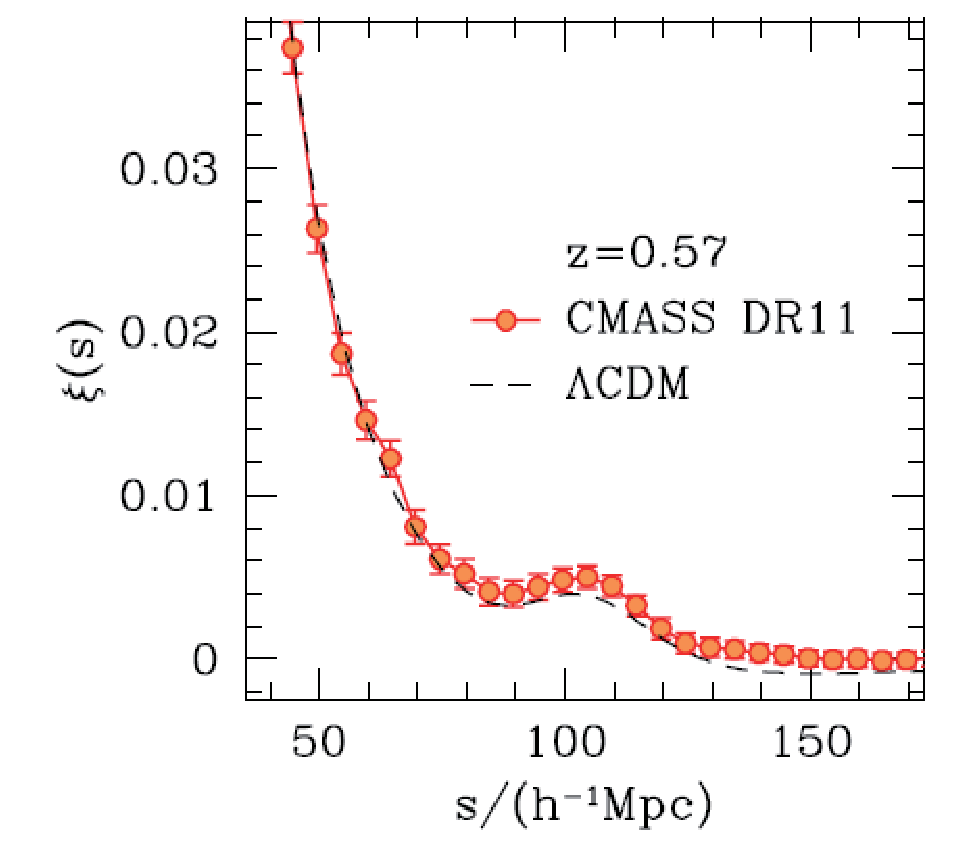
\includegraphics[width=0.95\linewidth]{cosmology/SDSS_BOSS_DR11_BAO.eps}   
   \caption{SDSS-III BOSSサーベイ(DR11)による角度平均した銀河の相関関数$\xi$~\citep{Sanchez:2013tga}。
            横軸は距離のスケールを表し、$100{\rm h}^{-1}{\rm Mpc}$付近にバリオン音響振動による
            ピークが見える。なお$\Lambda$CDMとは標準宇宙モデルのことである。}\label{fig:BOSS_BAO}
 \end{center}
 \end{minipage}
 \hspace{5pt}
 \begin{minipage}{0.5\hsize}
 \begin{center}\vspace{-10pt}
   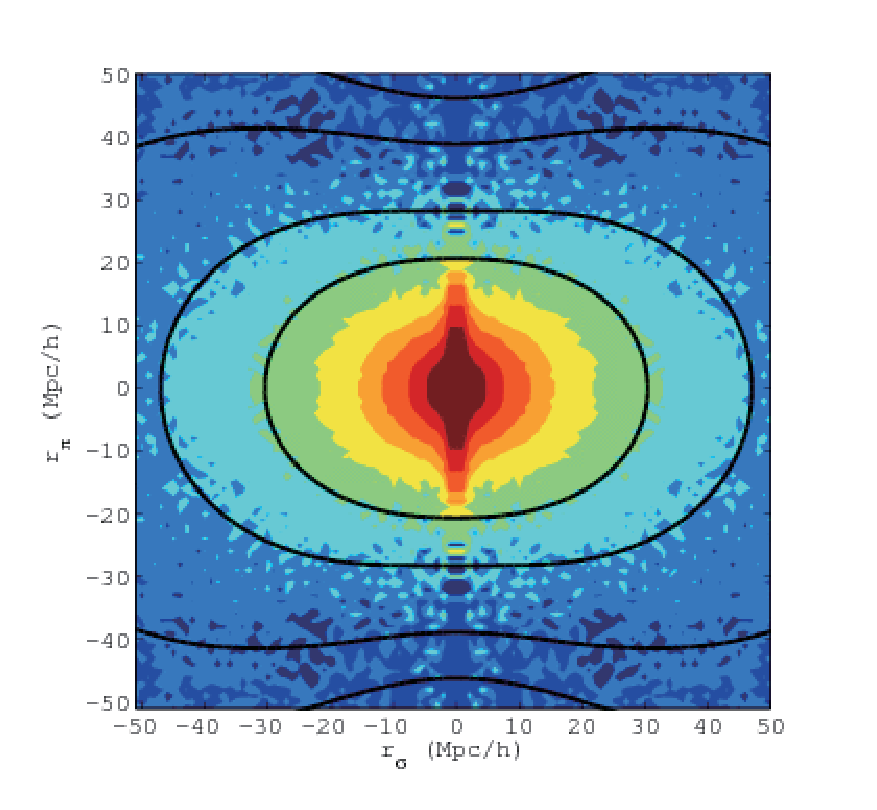
\includegraphics[width=0.95\linewidth]{cosmology/butterfly_colour_smallerscales.eps} 
   %\vspace{10pt}
   \caption{SDSS-III BOSSサーベイ(DR9)による、銀河の相関関数(赤いほど相関関数が大きい)~\citep{Reid:2012sw}。
           縦軸は視線方向、横軸は天球面上での距離スケールである。
           この縦方向と横方向における歪みが、赤方偏移空間歪みである。
           }\label{fig:BOSS_RSD}  
 \end{center}
 \end{minipage}
\end{figure}
%%%%%%%%%%%%%%%%%%%%%%%%%%%%%%%%%%%%%%%%%%%%%%%%%%%%%%%%%%%%%%%%%%%%%%%%%%%%

加えて、銀河の相関関数の非等方性として観測されるRSDも非常に有用な手法として
盛んに利用されている。赤方偏移空間歪みとは、個々の銀河の固有速度によって生じた赤方偏移による効果で、
たとえ実空間における銀河の分布が等方であっても、実際に観測される赤方偏移空間上では非等方な揺らぎとなってしまうことから発生する(図~\ref{fig:BOSS_RSD})。この固有速度の影響は、密度揺らぎの成長率と関係づくため、その成長に対する暗黒エネルギーの影響を調べることに利用することができる。

最後に、弱重力レンズ効果を利用した方法を説明する。
重力レンズ効果は、サーベイ対象の銀河からの光が経路上の物質による重力によって経路が直線からズレることで発生する。
その中でも弱重力レンズ効果とは、物質の重力によって発生する重力レンズ効果の内、
像の歪みが小さいために単独の観測対象を見ているだけでは
その影響が分からないもののことを呼ぶ。
したがってこの弱重力レンズ効果は、多数の観測対象を統計的に処理することで、
初めてその効果を測定することが可能となる。
%
この弱重力レンズ効果は宇宙の物質分布つまり密度揺らぎの情報を保持しており、
暗黒物質のエネルギー密度や暗黒エネルギーが密度揺らぎの成長に与える影響などについて、
詳細に調べるために利用することができる。

%%%%%%%%%%%%%%%%%%%%%%%%%%%%%%%%%%%%%%%%%%%%%%%%%%%
\vspace{15pt}

%%%%%%%まとめ%%%%%%%%%%%%%%%%%%%%%%%%%%%%%%%%%%%%%%

以上の様に、宇宙論における未解決問題であるインフレーションの検証、暗黒エネルギーおよび暗黒物質の正体の特定に向け、
様々な観測手法を用いることで宇宙論研究が行われている。
ここまで挙げた観測手法による宇宙論は、これまではほとんど光赤外観測によって推進されてきた。
将来観測(電波以外の波長については次節参照)により、これらの理解は格段に進歩することが予想される。
しかし、今後はSKAが登場することで電波によりこれらの観測を行うことが可能になり、電波観測によるこれまでにない規模・精度の
宇宙論を行うことができるようになる。
これにより、理論・観測両方面における宇宙論分野の更なる発展が期待される。

\subsection{他波長の将来計画}\label{cosmology.s1.ss2}

\subsubsection{マイクロ波背景放射}
これまで、COBEによる黒体輻射スペクトルの精密測定、地平線を超えた温度揺らぎの検出に始まり、DASIによるEモード偏光の検出~\citep{Kovac:2002fg}, WMAP衛星~\citep{Bennett:2012zja}, Planck衛星~\citep{Ade:2013zuv}による温度揺らぎの精密観測による宇宙論パラメタの決定、最近ではSPTPol~\citep{Hanson:2013hsb}, PolarBear~\citep{Ade:2013hjl}両実験による重力レンズ由来のBモード偏光の検出、さらにはBICEP2実験による重力波由来のBモード偏光の検出~\citep{Ade:2014xna}と、CMB実験はここ10年で急速な進展を遂げている。2014年末のPlanck衛星の偏光揺らぎの観測結果の発表をもって線形段階の密度揺らぎに由来するCMB温度揺らぎ・偏光揺らぎの観測は一段落を迎えることになる。%このPLANCKの結果次第でもあるが、その後の
今後のCMBの観測的研究の方向は大きく以下の4つが考えられる。
(観測計画リストは\ref{table:CMB future plan}参照)


\paragraph{重力波由来のBモード偏光スペクトルの詳細観測}
BICEP2によって報告されたBモード偏光検出については主要な観測が$1$周波数帯のみでしか行われておらず、前景放射のもれこみの問題が指摘されている\citep{Flauger:2014qra,Mortonson:2014bja}。Planckの複数の周波数帯による偏光観測により前景放射の情報が得られることが期待されているが~\citep{Adam:2014bub}、もしBICEP2の検出したシグナルが前景放射によるものだった場合、これまで以上に感度を上げた観測が必要となる。また、インフレーション由来の重力波であることを結論付けるためには、再イオン化によるバンプや整合性条件のチェックなど、広いスケールに渡ってスペクトルを観測する必要があり(例えば\citep{Dodelson:2014exa})、大角度スケールの観測に特化した地上観測や、衛星観測が必要になる。


\paragraph{重力レンズ由来のBモード偏光観測}
CMB弱重力レンズ効果は、宇宙晴れ上がり時の温度・偏光揺らぎの分布が、手前にある大規模構造による重力ポテンシャルによって歪められることによって発生する。特に密度揺らぎ起源であるEモードがレンズ効果によりBモードに変換されるが、このBモードは小スケールで他からのシグナルを卓越するため、重力ポテンシャルを再構築するのに適している\citep{Okamoto:2003zw,Hirata:2003ka}。重力レンズ効果によって推定される大規模構造は宇宙に存在する物質と重力の情報を含むため、例えばニュートリノ質量の精密測定や重力理論の検証などに用いることができる。


\paragraph{スニヤエフ・ゼルドビッチ(Sunyaev-Zel'dovich; SZ)効果}
大規模構造に付随する高温プラズマ(主に銀河団)はCMB光子を電子の熱運動によって逆コンプトン散乱することにより、CMBの黒体放射を歪ませる(熱的SZ)。この歪みの大きさは高温ガスの内部エネルギーに比例するため、重力ポテンシャルすなわち銀河団の質量のよい指標になる。また、この歪みは高周波側では温度の上昇、低周波側では温度の下降として観測され、温度揺らぎの観測からも検出することができる。一方、宇宙の再イオン化期に生成されるイオン化領域によるコンプトン散乱はその領域の特異速度に依存したドップラー効果により新たな温度揺らぎを生み出し(動的SZ)この効果を観測することにより、宇宙再イオン化期の情報(再イオン化開始時刻や時間など)を得ることが期待できる。


\paragraph{スペクトル歪みの詳細観測}
角度揺らぎとは別の方向性として、CMBのプランク分布からのずれの詳細な観測が計画・議論されている。宇宙初期における熱浴への熱流入は時期によって$\mu$歪み・$y$歪みを引き起こし、この歪みを詳細に観測することにより初期宇宙での物理過程を調べることができる。物理過程には、スニヤエフ・ゼルドビッチ効果の他に例えば粘性散逸による加熱や、ダークマターの崩壊、初期磁場の散逸などがある~\citep{Tashiro:2014pga}。


\begin{table}
 \centering
 \begin{tabular}{c|l|cccc}\hline\hline
  種類 &  \hspace{2zw}計画名\hspace{2zw} & 重力波 & 重力レンズ & \hspace{0.5zw}SZ\hspace{0.5zw} & スペクトル歪み \\\hline
  \multirow{4}{*}{人工衛星}
  & COrE+ & \checkmark & \checkmark & \checkmark \\\cline{2-6}
  & EPIC-IM & \checkmark & \checkmark & \checkmark & \\\cline{2-6}
  & LiteBIRD & \checkmark & & & \\\cline{2-6}
  & PIXIE & \checkmark & & & \checkmark \\\hline
  \multirow{5}{*}{バルーン}
  & EBEX* & \multirow{2}{*}{\checkmark} & & & \\
  & EBEX6K & & & & \\\cline{2-6}
  & LSPE & \checkmark & & & \\\cline{2-6} 
  & PIPER* & \checkmark & & & \\\cline{2-6} 
  & \textsc{Spider}* & \checkmark & & & \\\hline
  \multirow{17}{*}{地上}
  & ABS* & \checkmark & & & \\\cline{2-6}
  & ACTPol* & \multirow{2}{*}{\checkmark} & \multirow{2}{*}{\checkmark} & \multirow{2}{*}{\checkmark} & \\
  & AdvACTPol* & & & & \\\cline{2-6}
  & B-Machine* & \checkmark & & & \\\cline{2-6}
  & CLASS* & \checkmark & & & \\\cline{2-6}
  & GLP & \checkmark & & & \\\cline{2-6}
  & GroundBIRD & \checkmark & & & \\\cline{2-6}
  & Keck array* & \multirow{2}{*}{\checkmark} & & & \\
  & BICEP3* & & & & \\\cline{2-6}
  & MuSE & \checkmark & & & \\\cline{2-6}
  & \textsc{Polarbear}* & \multirow{3}{*}{\checkmark} & \multirow{3}{*}{\checkmark} & & \\
  & \textsc{Polarbear-2}* & & & & \\
  & Simons Array* & & & & \\\cline{2-6}
  & QUBIC* & \checkmark & & & \\\cline{2-6}
  & QUIJOTE* & \checkmark & & & \\\cline{2-6}
  & SPTpol* & \multirow{2}{*}{\checkmark} & \multirow{2}{*}{\checkmark} & \multirow{2}{*}{\checkmark} & \\
  & SPT-3G* & & & & \\\hline\hline
\end{tabular}
\caption{各CMB観測に関する星取表。*印は観測予定または観測中のもの。
ただし、重力波に関しては各実験が「low-$\ell$をターゲットにしている」「low-$\ell$を観測出来る」と明記しているもの、
重力レンズに関しては独自に重力レンズ角度パワースペクトルを評価できるだけチェックマーク( $\checkmark$ )を付けている。
監修:茅根氏}
\label{table:CMB future plan}
\end{table}



\subsubsection{光赤外}

宇宙論を主なターゲットにした光赤外サーベイは数多く計画されている。主要なアプローチとしては、弱い重力レンズの統計、銀河などの天体の空間分布の相関関数によるバリオン音響振動や赤方偏移空間歪みの効果、Ia型超新星爆発などが用いられる。観測装置としては地上望遠鏡と宇宙望遠鏡を使う方法に大別される。宇宙望遠鏡は大気の窓を越えてしか観測できない中間・遠赤外線の場合には地上では難しい高空間分解能や高感度を達成しうるという利点はあるが、一方で大口径の望遠鏡や超広視野の撮像装置、大掛かりな分光装置などを宇宙に打ち上げるのは非現実的であるので地上の大型望遠鏡も相補的な重要な役割を果たす。サーベイ観測には撮像サーベイと分光サーベイがあり前者は主に重力レンズやIa型超新星爆発、後者は主に銀河相関関数を用いた宇宙論を目指しこれらも相補的である。

撮像サーベイで$2020$年頃までの主力となるのは、すばる$8$m望遠鏡を用いた日本の Hyper Suprime-Cam (HSC) サーベイとアメリカが主導するチリの4m望遠鏡を使ったDark Energy Survey (DES) である。HSCは$1400$~deg$^2$の領域を$r\sim 26$等の深さで観測するのに対して、DESは$5000$~deg$^2$の領域を$r\sim 25$等とやや浅く観測していく。両者ともサーベイ観測を開始したばかりであり$5$年かけてサーベイを行っていく。

$2020$年以降に主力となる次世代サーベイはEuclid (Europian Space Agency (ESA))、WFIRST-AFTA (NASA)、Large Synoptic Survey Telescope (LSST; アメリカ) である。EuclidとWFIRST-AFTAは宇宙望遠鏡であり、地上からは感度が悪い近赤外での観測に重点がおかれている。また宇宙での観測は高空間分解能の画像が容易に得られるので弱い重力レンズで必須となる銀河の精確な形状測定の上で多くの利点がある。実際にEuclidは$15000$~deg$^2$の$r\sim25 $等の撮像データを用いた重力レンズ宇宙論を主なターゲットとしている。WFIRST-AFTAは多目的宇宙望遠鏡ではあるが$2000$~deg$^2$程度の領域をEuclidよりも深く観測し弱い重力レンズなどに用いることが予定されている。また遠方のIa型超新星爆発を狙った超新星サーベイも計画されている。LSSTはチリに$8$mの専用望遠鏡を設置しサーベイ観測を行う。LSSTは南天の$20000$~deg$^2$の領域を観測するが、その大きな特長としては時間変動の大規模なサーベイを行う点にある。具体的にはLSSTは一回の撮像で$r\sim 24$等の浅い観測を行い、この観測を数日おきに何度も繰り返し、最終的には同じ空の領域を何百回と観測し最終的な撮像データは$r\sim 27$等に達すると見積もられている。これにより時間変動する天体、例えば超新星爆発やクエーサーといった天体を全天規模で大量に発見することができ、時間変動天体に対する理解が圧倒的に進むであろうと期待されている。これに関しては東京大学で計画されているThe University of Tokyo Atacama Observatory (TAO)も重要な寄与をすると期待される。この大規模な時間変動を利用した宇宙論研究、たとえばIa型超新星爆発の統計解析や強い重力レンズの時間の遅れの研究などで大きな進歩が期待できる。

一方将来の分光サーベイとしては、Sloan Digital Sky Surveyの第四期サーベイの一つ Extended Baryon Oscillation Spectroscopic Survey (eBOSS; $2014$年開始)、すばる望遠鏡に取り付けられる予定の多天体分光器 Prime Focas Spectrograph (PFS; $2017$年頃以降)などがあり、$2020$年以降には地上4m望遠鏡に多天体分光器を取り付けるアメリカの計画 Dark Energy Spectroscopic Instrument (DESI) もある。またEuclidとWFIRST-AFTAの宇宙望遠鏡にもスリットレス分光機能が搭載され分光サーベイ観測を行う予定である。これらの分光サーベイの一番のターゲットはバリオン音響振動の観測による角径距離とハッブルパラメータの精密測定であり、これら将来計画により$0<z<3$の範囲で距離を1\%以下で測定しダークエネルギーの状態方程式に厳しい制限をつけることを目指す。

またこれらサーベイ観測と並んで、地上に$30$m級の大型望遠鏡を作る動きもある。アメリカや日本が主導する Thirty Meter Telescope (TMT)もその一つであり、ハワイに$30$m望遠鏡に設置し$2021$年稼働開始を目指している。ヨーロッパが主導するチリに$39$m望遠鏡を設置する European Extremely Large Telescope (E-ELT)、アメリカなどの同じくチリに$22$m望遠鏡を設置するGiant Magellan Telescope (GMT) も同時期の$2020$年頃の稼働を目指している。これらの大型望遠鏡は、暗い遠方銀河の分光観測による測光的赤方偏移の較正、遠方超新星爆発や強い重力レンズなどの宇宙論的に重要な天体の分光や補償光学を用いた高空間分解能撮像などの場面で活躍すると期待され、宇宙論研究にやはり重要な役割を果たす。



\subsubsection{X線}
X線観測による宇宙論の研究では、銀河団・銀河群の探査を行い、光赤外の観測による重力レンズ効果・電波観測によるSZ効果などから較正を行った推定質量を用いて銀河団・銀河群の質量関数と理論的なダークマターハローの質量関数を比較することで、宇宙論パラメータ・原始非ガウス性・重力理論などに制限を課すことが行われている。X線観測衛星のミッションは大きく分けて、銀河団・銀河群の大規模なカタログを作るsurvey型のミッションと、個々の銀河団を詳しく調べて推定質量の較正に役立てるobservatory型のミッションに分けられる。SKAが運用されるまでの今後$10$年間に計画されているX線観測衛星計画で、宇宙論的な文脈での研究が中心的なサイエンスを占めるものを以下に列挙する。
\begin{itemize}
\item ASTRO-H (日本・observatory型)\\
$2015$年秋に打ち上げ予定の日本のX線観測衛星で、世界で最初のTranslation Edge Sensor (TES)カロリメータを用いたX線分光装置 Soft X-ray Spectrograph (SXS) とCCDカメラSoft X-ray Imager (SXI) を用いた銀河団とその外縁部のX線観測が特徴的。
\item eROSITA on Spektr-RG (Russia, Germany・survey型)\\
ロシアとドイツが共同開発するSpektr-RGというX線観測衛星の観測装置の一つ。2014年Q3に打ち上げ予定だったが2015年に延期。有効面積の大きなX線望遠鏡とX線CCDの組み合わせで、X線での全天サーベイを行い銀河団とAGNのカタログを作成する予定。
\item DIOS (日本・observatory型)\\
ダークバリオンの大半を占めると考えられるWarm-Hot Intergalactic Medium (WHIM) 探査に特化したX線観測衛星。Diffuse Intergalactic Oxygen Surveyorの略。JAXA/ISASのイプシロンロケットを用いた小型科学衛星シリーズでの打ち上げを検討中。ASTRO-Hの$200$倍以上という非常に大きなグラプス(望遠鏡の有効面積と視野の積)を持つX線望遠鏡、TESカロリメータを用いた高いエネルギー分解能(5eV以下)のX線分光装置が特徴で$2020$年ごろの打ち上げを予定。
\item ATHENA (ESA)\\
ESAが計画中のX線観測衛星で$2028$年打ち上げ予定。eROSITAの更に$10$倍以上の有効面積を持つWide Field Imager (WFI)とTESカロリメータを用いた高いエネルギー分解能をもつX線分光器X-ray Integral Field Unit (X-IFU)を搭載し、これまでにない深いX線観測を行うことが可能になる。銀河団に関しては、赤方偏移が$1$を超える宇宙での銀河団や銀河群を内部構造も含めて観測する。また、再電離期程度の遠方宇宙までの銀河中心ブラックホールを観測することで、巨大ブラックホールの成長を理解することを目指している。
\end{itemize}




\subsection{SKA pathfinderによる宇宙論}\label{cosmology.s1.ss3}

以下、SKAのpathfinderによる宇宙論に関連したサーベイ計画をまとめておく。

\subsubsection{continuum survey}
\begin{itemize}
\item ASKAP EMU\\
正式名称はEvolutionary Map of the Universeで全天の75\%を$10~\mu{\rm Jy/beam~rms}$の感度、10-15 arcsecの角度分解能でサーベイし、約7千万個の銀河を観測する。$z=1$までのstar forming galaxyを観測できると期待されている。周波数帯は700-1800 MHz。
\item WODAN\\
正式名称はWesterbork Observations of the Deep APERTIF Northern-Skyで、WSRT (Westerbork Synthesis Radio Telescope)に配備されたphased array feed受信機であるAPERTIFを用いたサーベイである。ASKAPで観測できない全天の25\%の領域を$10~\mu{\rm Jy/beam~rms}$の感度、15 arcsecの角度分解能で観測する。
\item MeerKAT MIGHTEE\\
正式名称はMeerKAT International GigaHertz Tiered Extragalactic Exploration Survey。1.4 GHzでASKAP EMUやWODANに比べて狭い領域を深く観測する。
\item LOFAR\\
30-80 MHzと110-240 MHzの低周波で観測する。Tier 1, Tier 2, Tier 3の3つのサーベイフェイズがある。
\end{itemize}

\subsubsection{HI survey}

\begin{itemize}
\item ASKAP WALLABY\\
正式名称はWidefield ASKAP L-Band Legacy All-Sky Blind Surveyで全天の75\%を観測し$z=0.26$までの銀河を$500,000$個観測できる見込み。
\end{itemize}



\input{cosmology/cosmology.s2.tex}
\input{cosmology/cosmology.s3.tex}
\input{cosmology/cosmology.bib.tex}
\input{cosmology/cosmology.author.tex}


\chapter{銀河進化}\label{galaxy}

\section{銀河の「進化」とは}

銀河は進化する。
この事実は、銀河研究が本格化した1970年代後半から現在に至るまで、銀河物理学の研究の
駆動力であり続けている。
にもかかわらず、銀河がどのように形成され、進化してきたかは定量的にはまだ解明にはほど遠い。
銀河の進化とは具体的に何を指すだろうか?

銀河を特徴づける物理量には実に様々なものがある。
質量に関連する諸量から見ていこう。
ダークマターを含む全質量(力学質量)、バリオンの質量、そのうちの
星が占める質量、様々な相のガスの質量(電離ガス質量、中性ガス質量、分子ガス質量)、
そして銀河を形作る星が単位時間にどのくらいの質量形成されるかを表す星形成率、星形成の結果
生成され、銀河の星間物質に供給される重元素の質量(金属量)、重元素が固体微粒子(ダスト)の
存在形態を取る量(ダスト量)と、これだけでも多くの物理量がある。

ダークマター以外の銀河の構成要素は、基本的に複雑かつ多様な輻射過程を通じて電磁波を放射する。
その結果、銀河は様々な波長の電磁波の形でエネルギーを放出している。
銀河全体の光を積分したときの単位時間、単位波長当たりのエネルギー放射量を銀河の単色光度(monochromatic 
luminosity)と呼ぶ。
単色光度(あるいは観測者が受けるフラックス密度)を波長の関数としてあらわしたものをスペクトルエネルギー
分布(SED)と呼ぶ\footnote{単にスペクトルと呼ぶ場合もあるが、波長分解能が高い場合を特に差していることが
多い。これに対してSEDというときは単色光度の概形を指している。}。
銀河の光度は波長に強く依存し、また銀河の形態(渦巻、楕円、不規則など)や星形成率、重元素量とも
密接に関連している。
X線は銀河内の星の残骸(X線連星)やブラックホールへの質量降着によるエネルギー解放現象(活動
銀河核AGNと呼ばれる)、あるいは銀河の高温ガスから放射される。
紫外線は新しく形成された大質量星、そして星の進化の最終段階である白色矮星といった高温の星からの
放射の集積である。
可視光線および近赤外線は質量の小さな星まで含めたあらゆる星の連続光、そして電離ガスからの輝線、
場合によってはAGNからの熱放射が寄与する。
中間赤外線、遠赤外線は銀河にある様々なサイズ、組成のダスト粒子に星からの紫外線、可視光線が
吸収され、再放射されるエネルギーが支配的である。
さらに、これに原子ガスからの微細構造線や分子輝線が加わる。
サブミリ波、ミリ波も同様にダスト放射が卓越するが、これに電離領域の自由電子による熱制動放射も
加わる。
ミリ波よりも長波長の電波では、熱制動放射よりも超新星残骸などの磁場による磁気制動
放射(シンクロトロン放射)が卓越する。
また、この波長では中性水素の電子と陽子のスピン状態に起因する波長21~cmの超微細構造線が
重要な放射である。
このほか、銀河内で生じる高エネルギー現象によるガンマ線も放射される。
そして、銀河全体の積分量だけでなく、銀河の各部分は異なったSEDを持っている。
渦巻銀河の中心、バルジ部分、円盤部では寄与する天体や卓越する輻射過程がそれぞれ異なるからである。
近年開発が進んでいる可視光・近赤外線波長域での面分光装置や、高空間分解能な観測を可能とする、
ミリ波・サブミリ波そしてセンチ波の大規模な干渉計装置である、ALMAやSKAが動き出そうとしている今、
これまで近傍銀河でしか検証できなかった、``空間分解したSED''の理解は、極めて重要な役割を果たすと
考えられる。

銀河を力学的な側面からみると、質量以外にも銀河のダークマターの角運動量、銀河の回転速度も
重要な物理量である。
SED同様、銀河を空間分解して構造に着目すると、渦巻銀河の渦状腕のパターンやその回転速度、
楕円銀河の局所的速度分散、その非等方性も銀河の内部力学を規定する。
矮小銀河の場合はコヒーレントなパターンがないことが多く、銀河の部分部分が異なった運動をして
いることも稀ではない(NGC~4449など)。
星形成に起因する超新星爆発によって、エネルギーが星間物質に与えられ、銀河の外にむけて運動する
銀河風という現象も知られている。
銀河のポテンシャルが深い場合は物質は減速し、銀河本体に戻ってくる。
これは銀河噴水(galactic fountain)と呼ばれる。
これに対し、矮小銀河のようなポテンシャルの浅い銀河では星間物質の流れは銀河の脱出速度を
超え、銀河の外に流出する。
この場合は銀河風(galactic wind)と呼ぶ。
どちらも銀河の質量収支に影響を与える、重要なガスの運動として注目されている。
後でも述べるが、銀河同士が衝突$\cdot$合体することは宇宙では頻繁に生じる。
銀河の大きさ($\sim 10$~kpc)に比べ、銀河間の平均距離がさほど大きくない($\sim 1$~Mpc)ためである。
銀河の質量に差がある場合は、小さな銀河が大きな銀河に吸収されたとみなせる。
この場合力学状態はさほど乱れないが、星形成率には強い影響を与え、また一時的に特徴的な外見を
呈する場合がある(シェル、リップル、ポーラーリングなど)。
同程度の質量の銀河が合体する場合は力学的な影響は極めて強く、もともと持っていた形態は
いったん完全に失われ、最終的に楕円銀河的な密度構造に落ちつくと言われている。
これに関連する有名な問題がある。
銀河を構成する星は無衝突系であることが知られており、星同士が2体散乱を起こすことは
事実上ないといってよい。
ところが、楕円銀河の密度ポテンシャルはどれも極めて似通っており、2体緩和よりもはるかに速い何らかの
緩和過程を考えなければ観測が説明できない。
この問題は現在も完全には解決されていないが、「激しい緩和過程」(violent relaxation)と呼ばれる
統計力学的過程が考えられている。
このような過程の結果、衝突銀河の最終的な``平衡''形状は楕円銀河の密度プロファイルとなる。
しかし実際の銀河は星だけではなく、衝突系であるガスも含んでいるため、星のみの系同士の合体とは異なる結果を生じる可能性もある。
例えば、ガス成分の多い銀河同士の合体(gas-rich merger)では、合体後に円盤銀河になりうる、という結果を報告している研究がある\citep{2002MNRAS.333..481B, 2005ApJ...622L...9S, robertson2008, 2009ApJ...691.1168H}。
そのため、衝突銀河のガスの分布$\cdot$運動
などの情報を調べることは、銀河進化を理解する上で極めて重要である。

これらに加え、これまで直接観測は難しかった銀河外からのガス降着や、古くて新しい問題として
知られる銀河への環境の影響(環境効果)も重要な量であろう。
環境効果が銀河の形態や性質に影響を与えることは様々な観測から知られており、今後も新たな
事実が発見されると期待される。

銀河の進化とは、これら実に多彩な物理量が宇宙年齢とともに変化していく現象を指す。
厳密には、1個の銀河に着目したときの物理量の時間変化、いわば銀河の個人的ヒストリーと
各宇宙年齢で統計的に見たときの銀河の平均的物理量の変化、つまり社会的ヒストリーの
2つの側面がある。
銀河進化研究では必要に応じてこの2つの立場を使い分けている。
宇宙論的な文脈からは、ダークマターが重力相互作用し、その構造の進化のなかで銀河が形成、
進化してゆくという立場から研究が進められる。
この場合は力学的な進化が重要である。
しかし、銀河の分野で最も注目されているのは、最初のガス塊から星が生まれ、そして初代の星が
死ぬことで重元素が供給され、次世代の星形成が促進されてゆくというサイクル、すなわち
星形成進化である。
化学組成もこれに伴って変化してゆくので、重元素量の進化のことは化学進化という特別な
用語で呼ばれる\citep{tinsley1980}。
これらに加え、最近では積分した星質量の進化も重視されている。
銀河全体の進化だけでなく、たとえば矮小銀河の質量降着や銀河になっていない残存ガスが
大規模構造のフィラメントから降着してくるなどの過程によって、銀河のバルジ-ディスク比も
進化してゆく。
銀河合体は劇的な形態の変化をもたらし、これも銀河進化の重要な側面とみなせる。
銀河の中心部には大質量ブラックホールが存在していることが多いが、このブラックホールへの質量降着が
時間変化することで、AGN活動性も進化する。
さらに、中心核ブラックホールとバルジの間に相関が存在することから、銀河の進化とブラックホールの
進化も関連していることが示唆されている\citep[e.g.][]{magorrian1998}。
これは銀河とブラックホールの共進化(co-evolution)として知られている現象である。
銀河進化という言葉は、このようなイメージでとらえるのがよいであろう。

ここ10年で、多波長による銀河探査が飛躍的に進展し、宇宙年齢の非常に早い時期まで
観測データが揃うようになってきた。
これによると、銀河の進化は上に述べた様々な物理量のうち、基本的に2つの物理量で決まっているらしい
ことが見えてきつつある。
銀河の星質量と、局所的な環境である。
現在標準となっている、宇宙項のある冷たいダークマター宇宙モデル($\Lambda$CDMモデル)が
予言する階層的構造形成シナリオでは、小さな構造単位(ダークハロー)が合体することによって
より大きなダークハローが形成され、ダークハローの重力ポテンシャル環境の中で銀河が形成されると
考えられている。
銀河形成期以前の宇宙では、バリオンはほぼ完全にガス相で存在する。
それが大規模構造のフィラメントに降着し、そしてハローの作るポテンシャルに落下して濃い分子雲を
作ることで星形成が始まる。
分子雲から初期質量関数に従って星が誕生する。
大質量星は温度が高く、光度も大きいため強い紫外線で周囲のガスを電離し、電離水素領域を
形成する。
これは星形成の観点からは阻害に働く高価である。
また大質量星は短いタイムスケールで超新星爆発を起こし、持っていたガスを星間空間に戻す際に
重元素やダストを供給し、それとともに熱エネルギーや衝撃波を星間物質に与える。
冷たいガスや分子雲はこのようなエネルギーインプットによって熱いガスとなり、星形成は停止して
しまう。
これに加え、AGNからの強烈な放射やジェットなども星間物質の冷却を妨げる。
これらはネガティブフィードバックと呼ばれ、星の形成が進むことで星の形成を阻害する方向に働く。
この意味で、星形成は自己制御的(self-regulating)であると言われることもある。
このように、ダークハローの影響とバリオン物質の複雑なフィードバック機構が銀河の星形成を制御しつつ
進化し、今日の銀河となるのである。
銀河の星質量の成長を完全に理解するためには、星形成の原料である中性ガスの複雑な物理
過程を解明する必要がある。
このように、銀河の形成進化と大規模構造進化の理解には、銀河中の中性ガスをなるべく多くの
銀河について、なるべく異なった様々な環境で、宇宙年齢の関数として理解することが不可欠である。

\section{銀河進化研究の現状 -- 伝統的方法論とその限界 --}\label{galaxy.s0.5}

銀河進化の星形成に関する側面は、1970年代後半にTinsleyらが銀河の星種族の進化に
基づく観測量の進化理論を提唱して以来、様々な観測量を用いて検証されてきた。
まず注目されたのが、銀河の星種族の構成である。
星の寿命が星の初期質量に強く依存することから、同時期に生まれた星の集団の色(カラー)は
大質量の星から先に死んでいくことにより、時間とともに変化する。
黎明期の銀河進化研究で重視されたのは、化学進化理論に基づく銀河のカラーの進化であった
\citep[e.g.][]{larson1974, larson1978, larson1980}。
この頃は、階層的構造形成モデルはまだ標準としての地位を確立しておらず、銀河進化は
ワンゾーンで古典的に時間進化すると扱われていた。
この場合、個々の銀河の進化 $\simeq$ 銀河の平均的進化といえる。
現代的視点からみるとまだ未成熟ではあるが、銀河の平均的進化を宇宙論的な体積平均で
捉える「宇宙の星形成史」という概念を初めて提唱したのは\citet{tinsley_danly1980}である\footnote{よく
誤解されているが、最初に提唱したのはPiero Madauでは{\bf ない}。}。
宇宙の星形成史は1990年代後半に深い銀河探査を用いて銀河の平均的進化の検証に使われ
始めて以降、爆発的な流行を呼ぶこととなった\citep[e.g.][]{lilly1996, madau1996}。
銀河のカラーに基づく進化の検証の利点はもちろん、非常に成功した天体物理理論である星の進化の
体系を用いた明快な議論ができることである。
しかし、銀河のカラーの変化は概して時間分解能が極めて低く、その年齢での星形成率を測定できない。
特に長寿命の星からの輻射が卓越してくる銀河年齢($< 数{\rm Gyr}$)では顕著である。
このため、寿命の短い大質量星起源の物理量を用いる方法がこれに取って代わることになった。

大質量星は上記のように電離水素領域(H{\sc ii}領域)を形成する。
H{\sc ii}領域では水素の電離再結合が生じるため、Lyman, Balmer, Brackett系列など
水素の再結合線が放射される。
水素の再結合線強度は電離光子の数から量子力学的に正確に計算できるため、第一原理に
基づくクリアな議論がやはり可能である。
観測から再結合線の強度を測定して電離光子の数に換算し、そして星の輻射の理論から大質量星
(OB型星)の数(あるいは総質量)に焼き直す。
これに初期質量関数を仮定することで、大質量星の総質量は全質量の星の質量に換算できる。
こうして得られた星の質量は、大質量星の寿命のタイムスケール($10^6$~yr)の時間に形成された
星の全質量、つまり星形成率を表している\citep{kennicutt1983}。
これが銀河の進化のタイムスケールに比べて十分短いことから、銀河進化を議論する主要なツールと
して広く用いられている。
水素の再結合線のうち、最も進んでいた可視光線での観測に都合がよいのがBalmer系列の
輝線(H$\alpha$、H$\beta$、H$\gamma$など)である。
Lyman系列は紫外線であり、赤方偏移が高い銀河では可視光で観測できるため、10~mクラスの
光学望遠鏡が建造されるようになってから銀河進化研究によく用いられるようになった。
また、大気吸収や夜光によって地上空の観測が難しかった近赤外線のBrackett系列も、観測
装置の発展により今日では星形成率の研究に用いられている。
赤方偏移が1--2付近の銀河ではBalmer系列がこの地球大気による邪魔の多い波長にシフトするため
観測が困難であることから長く「赤方偏移砂漠」(redshift desert)と呼ばれていたが、同様に
近赤外線観測装置の発展によりこの問題も解決に向かっている。
ところが、水素再結合線による星形成の評価は万能ではない。
\citet{kennicutt1983}の中ですでに議論されているように、銀河の星形成は必ずダストの
生成を伴う。
可視光線および紫外線はダストの減光\footnote{ダスト粒子による散乱と吸収の効果の総称をこう呼ぶ。}の効果を
強く受けるため、観測量からそのまま算出した星形成率は常に過小評価である。
この問題は早い時期から認識されていたものの、銀河進化、特に紫外線に根拠を置く研究者の間では
軽視され続け、その結果銀河の星形成進化についての理解の混乱を引き起こすことになった。

ダスト粒子は星が形成され、大質量星が超新星爆発を起こすタイムスケールで生成される。
このためダストは星形成領域には必ず存在している。
ダストが吸収した紫外線のエネルギーはダスト粒子からの熱放射として主に中間--遠赤外線で再放射
されるので、ならばむしろ赤外線放射光度を大質量星からの電離光子の指標として用いることが
考えられる\citep[e.g.][]{1998ARA&A..36..189K}。
ダストによる吸収が顕著な銀河では、この方法は星形成の指標として有効である。
遠方宇宙においてダストで強い吸収を受け、巨大な赤外線光度を持つ銀河が発見されたことで、
星形成率の指標としての赤外線は急激に注目されることになった\citep[e.g.][]{hughes1998}。
高光度赤外銀河と呼ばれるこの種族は、1個当たりの星形成率が極端に高い(100--1000~$M_\odot\,{\rm yr}^{-1}$)
ため、宇宙の星形成率への寄与が大きい可能性が指摘され、星形成率はむしろ赤外線のみで
測定すれば足りるという極端な見方をする研究者も出てきた。
しかし当然ながら紫外線のみ、赤外線のみではどちらも不十分な情報しか得られないことは自明である。
\citet{takeuchi2005}は$0 < z < 1$の宇宙で紫外線と赤外線の光度関数をもとめ、これらを積分することで
全星形成率への双方の寄与を評価した。
その結果、近傍宇宙ではほぼ同じ寄与となるものの、$z=1$の宇宙では90~\%以上の星形成がダストで
隠されており、赤外線でしか観測できないことを見出した。
この結果はその後の研究により$z \simeq 4$まで検証され、$1 < z < 3$の宇宙ではこの隠れた星形成が
支配的であることが確定的となった\citep[e.g.][]{cucciati2012, burgarella2013}。
とはいえ、双方の情報を用いた星形成率指標が理想的であることは言うまでもなく、現在ではそのような
指標がいくつか提唱され、評価されている\citep[e.g.][]{kennicutt2009,takeuchi2010,murphy2011}。
このうち、電波連続波もダストの影響を受けない星形成率の指標として使われており、電波連続波で探る銀河進化は、
SKAの重要なサイエンステーマの一つである (詳細は\S~\ref{sec:continuum}参照)。

その他の星形成率を評価するための観測的指標としては、X線連星起源の光度、H{\sc ii}領域からの禁制線
([O{\sc ii}]など)の光度、多環式芳香族炭化水素のバンド輝線光度、非電離紫外線連続光光度や
シンクロトロン放射光度などが用いられている。
ところが、これらはすべて星形成率を測る指標であり、銀河形成と成長のキーである「ガスから星への変換」に
ついては何も語ってはくれない。
これに対し、電波天文学では分子輝線を用いた分子ガス量が星形成に関連する測定量として
精力的に研究されてきた。
こちらはある時刻における銀河が持つ「星形成の材料」の量を示している。
これと星形成率を組み合わせることで、ガスから星への過程を議論することができる。
しかし、分子輝線はすでに分子雲になったガスをトレースするのみであり、更にこれをおしすすめて中性ガスまで
含めた議論をする必要がある。
これまではH{\sc i}の21~{\rm cm}輝線が観測できる赤方偏移がほぼ近傍宇宙に限られていたため、銀河進化の
観点から議論されることは稀であった。
SKAはこれを可能にし、銀河進化研究に絶対的なブレイクスルーを与えることになる。


\section{銀河進化研究の現状 -- 銀河におけるHIガス --}\label{galaxy.s1}

%%%%%%%%%%%%%%%%%%%%%%%%%%%%%%%%%%%%%%%%%%%%%%%%%%%%%%%%%%%%%%%%%%%%%%%%%%
\subsection{水素原子と水素分子}\label{sec:HI_H2}
%%%%%%%%%%%%%%%%%%%%%%%%%%%%%%%%%%%%%%%%%%%%%%%%%%%%%%%%%%%%%%%%%%%%%%%%%%

銀河において星形成の材料となるのは分子ガスである。銀河系では、
星間物質のうち質量の約半分が分子ガス、特に水素分子(H$_2$)ガスになっていることが知られている。
この小節では銀河における水素分子の生成および解離と、水素分子と水素原子(H {\sc i})
の割合について述べる。
SKAの観測では、原子ガスが重要な観測対象となるが、原子と分子の二相は下で
見る様に密接に関係しており、両方の理解が重要である。

\subsubsection{水素分子の生成}
銀河において、水素分子の最も基本的な生成過程は2つの水素原子による共役反応で、電子や陽子を触媒として起こる。この共役反応では水素分子の生成に伴って多量の発熱エネルギーが生じる。この発熱エネルギーを捨て去られない限り反応は逆戻りするため水素分子は生成できない。
水素分子生成に伴う発熱エネルギーを捨て去るためには3つの水素原子による衝突反応が必要となる。この衝突反応では3つ目の水素原子が余分な発熱エネルギーを持ち去ってくれるため、水素分子を生成することができる。このような3つの水素原子による水素分子の生成は、非常に高密度な環境($n_{\text{H}}>10^8$ cm$^{-3}$)で促進される。しかし実際の銀河では、銀河系の分子雲でさえ水素原子の平均的な個数密度が$n_{\text{H}}\sim10^5$ cm$^{-3}$以下という低密度環境であるため、水素原子の衝突反応による水素分子生成はほとんど起こらない。

銀河において最も効率のよい水素分子生成は星間塵を触媒とする
方法である\citep{1963ApJ...138..393G, 1971ApJ...163..155H}。
星間塵の内部では様々な運動モードが存在している。そのため、星間塵表面で水素分子が生成されると、生成で生じた発熱エネルギーは星間塵が熱浴となって吸収してくれると考えられる。

星間塵表面での水素分子形成過程は、1) 水素原子の星間塵表面への付着過程、2) 星間塵表面での拡散過程、3) 星間塵表面での2つの水素原子の反応過程、4) 生成した水素分子の星間塵表面からの離脱過程の4つの素過程にわけて考えることができる(図\ref{fig:grain})。まず、気相中を漂っているある水素原子が星間塵の表面に付着する(過程1)。この時水素原子が星間塵に付着できるかどうかは、水素原子の星間塵への衝突エネルギーと星間塵からの脱出エネルギーのバランスで決まる。衝突エネルギーが星間塵に十分に吸収され、星間塵表面からの脱出に要するエネルギーを満たさなければ水素原子は付着できる。
付着した水素原子と星間塵表面の間に働く結合力(Van der Waals力)は弱い。そのため、水素原子は星間塵表面上を動き回り、やがてポテンシャル場の井戸に落ち込む(過程2)。
次に別の水素原子が星間塵表面に付着し、最初の水素原子同様に表面上を動き回る。しばらくすると、この水素原子はポテンシャル場にいる最初の水素原子と出会い、水素分子を生成する(過程3)。分子動力学シミュレーションによると、この水素分子生成の反応には2つのパターンが見られる\citep{1999MNRAS.306...22T}。
1つ目は上述の星間塵表面上での2つの水素原子により引き起こされるパターン、2つ目は星間塵表面に付着している水素原子へ気相中の別の水素原子が直接衝突をして反応を起こすパターンである。
いずれかの反応によって生成された水素分子は、星間塵表面における結合エネルギーを切り、気相として星間塵表面から離脱する(過程4)。
星間塵表面での水素分子の生成率は、太陽系近傍の分子雲で$k\sim 3 \times 10^{-17} \; \mbox{cm}^3\, 
\mbox{s}^{-1}$であるといわれている\citep{1975ApJ...197..575J}。


%%% Figure
\begin{figure}[tbp]\label{fig:grain}
\begin{center}
\includegraphics[width=\linewidth]{galaxy/h2form.eps}
\end{center}
\caption{星間塵表面における水素分子生成の4つの素過程(高橋 2000)。}
\end{figure}
%%%

\subsubsection{水素分子の解離}

一度生成された水素分子も何らかの原因で解離され、再び水素原子に戻ることがある。この水素分子の解離を引き起こす原因は大きく3つあげられる。
まず1つ目は、主にO型星と一部のB型星から放射される$11.2-13.6$ eVの紫外光子(Lyman-Werner光子)による光解離である。 このような放射場の周囲では、水素分子のみで構成された分子雲は光解離によって水素分子から水素原子へ解離されてしまう。
しかし、分子雲が非常に高い柱密度をもつ場合($N_{{\rm H}_2}>10^{14} \; \mbox{cm}^{-2}$)、その内側は自己遮蔽によって光解離を免れる\citep{1996ApJ...468..269D}。
また、分子雲中に星間塵が含まれていた場合も紫外光子は星間塵によって吸収・散乱されるため、分子雲の内側は光解離の影響を受けない。このような光解離を免れた分子雲の内側で新しい星が形成されると考えられている。

2つ目は$1\mbox{--}100$~MeV程度の陽子である宇宙線による解離である。
宇宙線は星間塵の影響を受けず、分子雲を貫くことができる。そのため、分子雲の中心部の水素分子を電離させる。この反応は水素分子の宇宙線電離とも呼ばれる:
	\begin{eqnarray}
		\text{H}_2		+ (宇宙線) 	& \rightarrow & \text{H}^+_2 	+ e^-	+ (宇宙線) .
%									& \rightarrow & \text{H}^+		+ H		+ e^-	.
	\end{eqnarray}
この反応によって生じたH$_2^+$イオンは周囲の水素分子とただちに反応してプロトン化水素分子(H$^+_3$)を生成する。
	\begin{eqnarray}
		\text{H}_2^+	+ \text{H}_2	& \rightarrow & \text{H}^+_3 	+ \text{H}
	\end{eqnarray}
分子雲では、宇宙線電離によって生成されたH$^+_3$が他分子の生成に寄与することが知られている\citep{johnsen}。

3つ目の水素分子の解離過程は高温$\cdot$高密度な星間空間における衝突解離である。中性な星間空間では、水素分子の衝突解離は水素原子、ヘリウム原子、水素分子によって引き起こされる。
電離領域では、電子や陽子が水素分子の衝突解離を誘発する。また、速度が$v_s > 20\; \mbox{km} \, \mbox{s}^{-1}$をもつ衝撃波領域でも衝突解離が生じることが知られている\citep{1977ApJ...216..713K, 1977ApJ...217..442L}。
しかしこの衝突解離は水素分子解離の原因としての寄与は小さいと考えられる。理由としては、衝突解離によって水素分子生成で生じる熱エネルギーが効率よく捨て去られたり、星間空間中の金属による冷却を受け、水素分子の解離よりも生成が促進されるためである\citep[e.g.][]{1963ApJ...138..393G}。

\subsubsection{銀河における水素分子と水素原子}

銀河における水素分子と水素原子の割合(分子比率:$f_{\text{mol}}\equiv \rho_{{\rm H}_2} / \rho_{{\rm total}}$, $\rho_{{\rm total}}=\rho_{{\rm H}_2}+\rho_{\rm HI}$)は、水素分子の生成と解離のバランスで決まる。
\citet{1993ApJ...411..170E}は、$f_{\text{mol}}$が分子雲にかかる様々な圧力、紫外光子の放射場、金属量の関数として記述される解析的な1次元のモデルを提案した。
\citet{2008ApJ...689..865K}では、\citet{1993ApJ...411..170E}の分子雲を球対称モデルとして扱い、星間塵による水素分子生成をパラメーターとして加えた多次元の解析モデルを提案した。
これらのモデルは、銀河系や近傍銀河の観測結果をよく説明している\citep{1995A&A...296...33S, 1995A&A...304....1H, 2004ApJ...612L..29B, 2008AJ....136.2782L}。

観測的な$f_{\text{mol}}$の検証は、主に、銀河系や近傍銀河の$^{12}$CO($J=1-0$)輝線(2.6~mm)とH\,{\sc i}輝線(21~cm)の観測データをもとに行われている。$^{12}$CO($J=1-0$)輝線の観測からは輝線強度と水素分子柱密度の変換係数($X_{\text{CO}} \;\mbox{[cm}^{-2} \mbox{(K km s}^{-1})^{-1}]$)を介し水素分子の面密度が、H\,{\sc i}輝線の観測からは水素原子の面密度が得られる。これら面密度の比から$f_{\text{mol}}$は見積もられる。
円盤銀河で代表される晩期型銀河では、銀河全体として$f_{\text{mol}}\sim 25 \mbox{--} 30\; \%$に
なると報告されている\citep{2014A&A...564..66B}。
さらに、晩期型銀河における$f_{\text{mol}}$の動径分布を調べると、銀河中心から動径方向に減少することが知られている\citep[e.g.,][]{2012ApJ...756..183B, 2014PASJ...66...66T}。
図\ref{fig:leroy}は晩期型である渦巻銀河(NGC 628)における、中心からの水素分子・水素原子面密度の動径分布を表している。
水素分子は銀河中心部をピークに動径方向に面密度が小さくなっていく。一方、水素原子は銀河中心部では面密度が小さく、数kpc外側から(図\ref{fig:leroy}では半径$100''$付近)動径方向に面密度は徐々に大きくなる。そのため、晩期型銀河の$f_{\text{mol}}$は銀河中心部で1に近く、外側にいくにつれて小さくなるような分布を示す。

次に、水素原子から水素分子へ遷移する密度について記述する。
解析的な理論モデルによると、太陽の金属量をもつ球対称な分子雲の中では、光解離からの遮蔽が水素原子の面密度で$\Sigma_{\text{HI}} \approx 10\; M_\odot \mbox{pc}^{-2}$付近(柱密度で$N_{\text{H}}\sim 10^{21}\;
\mbox{cm}^{-2}$程度)で効くことが示唆されている\citep{2009ApJ...693..216K}。
水素分子の生成/解離を組み込んだ銀河形成進化の数値シミュレーションにおいても、同様の金属量をもつ銀河では$N_{\text{H}}\sim 10^{21} \; \mbox{cm}^{-2}$でほぼ全ての水素原子は水素分子へと遷移する
\citep[e.g.,][]{2006ApJ...645.1024P, 2009ApJ...697...55G}。
これら理論研究による予言値とほぼ等しい値が、太陽と同程度の金属量をもつ近傍の晩期型銀河の観測から得られている\citep[e.g.,][]{2002ApJ...569..157W, 2008AJ....136.2846B}。

しかし、水素分子へ遷移する柱密度は金属量によって変わりうる。Gnedin et al. (2009)では、金属量が低いほど水素分子へ遷移する柱密度が高くなることを示唆した。彼らのシミュレーションの中では金属量が低いと光解離を遮蔽する星間塵が少なくなる。そのため、光解離からの遮蔽が効く柱密度は高くなる。同様の結果は他の理論モデルや近傍銀河の観測からも得られており\citep[e.g.,][]{2009ApJ...693..216K, 2010ApJ...709..308M, 2010ApJ...722..919F, 2013ApJ...777L...4W, 
2014MNRAS.442.2780R}、金属量は水素原子から水素分子への遷移において鍵となるパラメーターと言える。

%%%%%%%%%%%%%%%%%%%%%%%%%%%%%%%%%%%%%%%%%%%%%%%%%%%%%%%%%%%%%%%%%%%%%%%%%%
\subsection{渦巻銀河のHIガス}
\label{sec:spiral}
%%%%%%%%%%%%%%%%%%%%%%%%%%%%%%%%%%%%%%%%%%%%%%%%%%%%%%%%%%%%%%%%%%%%%%%%%%

渦巻銀河の中性水素ガス(H\,{\sc i}ガス)の観測は1950年代に遡る。以来、電波単一鏡や干渉計
\footnote{2014年現在科学運用されている望遠鏡としては、電波単一鏡ではGreen Bank Telescope、Areciboが、干渉計ではVery Large Array (VLA)などがある。}
によって、非常に近傍($\sim50$ kpc)から、100 Mpc以上($z>0.024$)の銀河に至るまで広く観測されている。本小節では渦巻銀河におけるH\,{\sc i}ガス観測によってもたらされた物理的な理解についてまとめる。


\subsubsection{空間分布}\label{sec:distribution}
渦巻銀河におけるH\,{\sc i}ガスの分布には大きく3つの特徴が見られる。
1つ目の特徴は銀河中心部に見られる穴である。一般的に銀河中心部は高密度である。そのため、ほぼ全ての水素原子が水素分子に遷移してしまい、H\,{\sc i}ガスがほとんど存在していないことに起因していると考えられている($\S$\ref{sec:HI_H2}参照)

2つ目の特徴は、H\,{\sc i}ガスは可視光観測で得られる円盤部より顕著に広がって分布していることである\citep[e.g.,][]{1983IAUS..100...55S, 2008AJ....136.2782L}。
図\ref{fig:leroy}上側のパネルには近傍渦巻銀河(NGC 628)の可視観測より得られた星、H\,{\sc i}ガス、CO観測による分子ガスの空間分布が示してある。星や分子ガスは図中の黒点線で囲まれた円内に収まるのに対し、H\,{\sc i}ガスは円のかなり外側まで広がっていることがわかる。このように多くの渦巻銀河では、H\,{\sc i}ガスは星の円盤と比べ2--3倍以上広がっている\citep[e.g.,][]{1983IAUS..100...55S}。

渦巻銀河の外側に見られる広がったH\,{\sc i}ガスのような、星の円盤周囲にあるガスは銀河周辺ガス(circum-galactic medium: CGM)と呼ばれている。
CGMは、理論的には銀河間ガスの降着や銀河からのアウトフローに関連していると考えられており\citep[e.g.,][]{2002ApJ...571...40M, 2006Natur.440..644M, 2009Natur.457..451D, 2009ApJ...703..785D, 2005ApJ...635L..13S, 2011MNRAS.415..11D}、銀河の質量獲得過程や星形成史と密接に関連した重要な研究対象となっている。CGMのH\,{\sc i}ガスの柱密度は円盤部
\footnote{渦巻銀河円盤部のH\,{\sc i}ガス柱密度は$N_\mathrm{HI}\sim10^{20\mbox{--}21}$ cm$^{-2}$程度。}
と比べ低く($N_\mathrm{HI}<10^{19}$ cm$^{-2}$)、観測的な直接検出が課題であった。しかし近年の観測装置の性能向上により、高感度のH\,{\sc i}ガス観測が可能となり、CGMの淡いH\,{\sc i}ガス($N_\mathrm{HI}\sim10^{18}\; \mbox{cm}^{-2}$)が検出され始めてきた\citep{2013Natur.497..224W, 2014AJ....147...48P}。
このデータをもとに渦巻銀河へのガスの流入の議論が行われつつある。

3つ目の特徴は、H\,{\sc i}ガスの面密度($\Sigma_{{\rm HI}} [M_\odot \mbox{pc}^{-2}]$)が渦巻銀河の外側で比較的一定になることである。銀河中心から各半径における$\Sigma_{\text{HI}}$は、中心で低く(特徴1)、半径が大きくなるにつれて急に高くなり、ある半径でピーク($\Sigma_{\text{HI}}^{\text{max}}$)となる。
その半径より外側では、$\Sigma_{\text{HI}}$の動径分布は比較的平坦になる\citep[e.g.,][図\ref{fig:leroy}下参照]{2008AJ....136.2782L, 2012ApJ...756..183B}。
$\Sigma_{\text{H\,{\sc i}}^{\text{max}}}$は高くとも$\sim10$ $M_\odot$ pc$^{-2}$程度までしかあがらない。それは、$\Sigma_{\text{H\,{\sc i}}}>10$ $M_\odot$ pc$^{-2}$ではほとんどの水素原子は水素分子に遷移してしまうためである($\S$\ref{sec:HI_H2}参照)。

%%% Figure
\begin{figure}[t]
%\vspace{-4\baselineskip}
\begin{center}
\includegraphics[width=12cm]{galaxy/Leroy08.eps}
\end{center}
\caption{NGC 628のH\,{\sc i}ガス、分子ガス、星の画像と銀河中心からの動径分布(Leroy et al. 2008を修正し転載; 可視画像はSpace Telescope Science Instituteより)。物理的なスケールとして、$1''$は約35~pcに相当する。}
\vspace{1\baselineskip}
\label{fig:leroy}
\end{figure}
%%%


\subsubsection{H\,{\sc i}ガス質量}
21~cmで観測されるH\,{\sc i}ガスは光学的に薄く、次の関係式を用いて視線方向の輝線強度($I_\mathrm{HI}\; \mbox{[K km s}^{-1}$])から柱密度$N_\mathrm{HI}$を求めることができる。
	\begin{eqnarray}
		N_\mathrm{HI}~[\text{cm}^{-2}] = 1.823 \times 10^{18} \; I_\mathrm{HI}~[\text{K km s}^{-1}] 
	\end{eqnarray}
また、得られた柱密度を銀河の全領域で積分すると、銀河におけるH\,{\sc i}ガスの総質量を求めることができる。
観測データをもとに見積もられた渦巻銀河におけるH\,{\sc i}ガスの総質量は、$M_{\text{HI}}\sim10^{8\mbox{--}10} \; M_\odot$程度となる\citep[e.g.,][]{2008AJ....136.2563W}。
なかでも$M_{\text{HI}} \sim10^{10} \; M_\odot$近い値を示す渦巻銀河は衝突している銀河であり、銀河同士の衝突や相互作用によって多くの星間物質がもたらされた結果であると考えられている。

このように見積もられた渦巻銀河のH\,{\sc i}ガスの総質量と円盤部の大きさには相関が見られることが知られている。
$\S$\ref{sec:distribution}に記したように、渦巻銀河では$\Sigma_{\text{HI}}$が外側の半径でほぼ一定となる。そこで銀河全面にわたり$\Sigma_{\text{HI}}$が一定であると見なすと、渦巻銀河のH\,{\sc i}ガス総質量は銀河の面積にほぼ比例することになる。実際に、H\,{\sc i}ガスの総質量が主に星円盤の半径に依存していることが示唆されている\citep[e.g.,][]{2012ApJ...756..183B}。


\subsubsection{力学情報}
H\,{\sc i}ガスは渦巻銀河内の広域に分布しているため、その運動情報から銀河の質量分布を求めることができる。図\ref{fig:deblok08}には様々な渦巻銀河におけるH\,{\sc i}ガスの回転速度が距離の関数(回転曲線)として示されている。回転速度の大きさは平均的に$150-300$ km s$^{-1}$と銀河によって異なるが、基本的には回転曲線は中心から外側にいくほど速くなり、ある半径でほぼ一定($v_{\text{max}}$)に達するという平坦な分布を示す\citep[e.g.,][]{1980ApJ...238..471R, 1985ApJ...289...81R,1981AJ.....86.1791B, 1987IAUS..117...67S, 1987IAUS..124..699S}。
ここでH\,{\sc i}ガスは銀河内を回転曲線に従う円運動を行なうと仮定する。
この時、銀河の質量分布に回転対称性があると仮定し、半径$r$以内に含まれる質量を$M$($r$)、$r$での回転速度を$v(r)$とすると、重力と遠心力のつり合いから
%この時、銀河の質量分布が球対称であると近似すると、半径$r$以内に含まれる質量を$M$($r$)とするような質量と速度$v$($r$)は重力と遠心力のつり合いから
	\begin{eqnarray}
		\frac{v( r)^2}{r}	& = &	G \frac{M( r)}{r^2}
	\end{eqnarray}
のように書くことができる。この式を変形すると
	\begin{eqnarray} \label{eq:galrot}
		M( r)	& = &	\frac{rv( r)^2}{G}
	\end{eqnarray}
となり、回転曲線から質量分布$M$($r$)を求めることができる。このように回転曲線から見積もった質量を力学質量と呼ぶ。

%%% Figure
\begin{figure}[htbp]
\begin{center}
\includegraphics[width=14cm]{galaxy/Sancisi.eps}
\caption{様々な渦巻銀河の回転曲線(\citealt{1987IAUS..117...67S}を修正し転載)。$400\; \mbox{km s}^{-1}$を越える速い回転速度をもつ銀河は少ない。}\label{fig:deblok08}
\end{center}
\end{figure}
%%%

前述のように回転曲線は一般に半径に対してほぼ一定値をとることから、力学質量$M(r)$は半径に比例して増加することがわかる。また、回転速度が大きい銀河ほど総質量が大きくなることもわかる。
一方で、可視光や電波などの電磁波で観測される星やガス(H\,{\sc i}、分子)などの物質(バリオン)は銀河の外側にいくほど観測されにくい。これはバリオンの存在量が銀河の外側では少ないことを意味している。
%一方で、可視光や電波などの電磁波で観測される星やガス(H\,{\sc i}、分子)などの物質の分布は、 銀河の外側にいくほど暗く、存在量としては少なくなる。この違いは、
渦巻銀河の回転曲線から予想される力学質量と、観測から期待されるバリオン質量の不一致は、銀河の外側には観測されている物質以外に「見えない物質」が大量に存在していることを示唆している。この見えない物質をダークマターと呼ぶ。この、渦巻銀河の外側で見られる光学質量と力学質量の違いは銀河にダークマターが存在している一つの証拠となっている。


\subsubsection{タリー--フィッシャー関係}\label{sec:TF}

渦巻銀河の回転速度と真の明るさの間には``タリー--フィッシャー関係(TF関係)''と呼ばれる経験則がある\citep{1977A&A....54..661T}。
渦巻銀河の光度を$L$とすると、光度と回転速度($v_{\text{max}}$)の間には、$L\propto v_{\text{max}}^\alpha$($\alpha\approx4)$という関係が成り立ち、銀河における星成分とダークマター成分との関係を示す重要なスケーリング則である。
銀河の光度は銀河を構成する物質(主に星)の質量に比例するため、TF関係は銀河の星質量と回転速度の関係としても表すことができる。

TF関係は星質量が低い側において分散が大きくなることが知られている。これは、星質量が小さい渦巻銀河では星質量に対するガス質量の割合が無視できなくなるためである。そこで、星質量に加えガス質量も加えたバリオンの総質量($M_{\text{バリオン}} = M_* + M_{\text{ガス}}$)を用いることで、回転速度との相関が強くなる(分散が小さくなる)ことが示唆された\citep[e.g.,][]{2001ApJ...550..212B}。
この関係をバリオン-タリー--フィッシャー関係(BTF関係)という。
観測的には、近年行われている渦巻銀河のガス観測のサーベイデータを用い、BTF関係の検証が行われている\citep[e.g.,][]{2012AJ....143...40M}。

TF関係は渦巻銀河の距離を測定する指標としても使われている。
TF関係とH\,{\sc i}観測によって得られる銀河の回転速度から、銀河の真の明るさを見積ることができる。 一方、観測される銀河の明るさは距離に依存して変化する。そこで、銀河の真の明るさと観測される銀河の明るさの差を用いると、渦巻銀河までの距離を評価することができる。これまでは、H\,{\sc i}観測、星の分光観測それぞれで得られるTF関係から、渦巻銀河までの距離が調べられてきた。近年、特にBTF関係を用いることで高精度で距離決定ができることがわかってきた\citep[e.g.,][]{2001ApJ...550..212B}。しかし、観測的な星質量やガス質量の導出にはまだ多くの課題があり、その分、銀河までの距離決定にも不定性が生じうることに注意が必要である\citep[e.g.,][]{2014AJ....147..134Z}。

%%%%%%%%%%%%%%%%%%%%%%%%%%%%%%%%%%%%%%%%%%%%%%%%%%%%%%%%%%%%%%%%%%%%%%%%%%
\subsection{早期型銀河のHIガス}
\label{sec:早期型銀河の構造・運動・星種族}
%%%%%%%%%%%%%%%%%%%%%%%%%%%%%%%%%%%%%%%%%%%%%%%%%%%%%%%%%%%%%%%%%%%%%%%%%%


早期型銀河(楕円銀河・レンズ銀河)に関する従来の描像としては、バルジが卓越し(高いバルジ--ディスク比)、一様に古い星から構成されている、というものである。
しかし、バルジ--ディスク比がSc型渦巻銀河と同程度のものなど \citep{1951ApJ...113..413S,1970ApJ...160..831S,1976ApJ...206..883V}、早期型銀河にも形状の多様性があることが知られている。
また、大半の早期型銀河は、現在の星形成活動がほとんどないことが観測的に示されている \cite[e.g.,][]{1993PhDT.......172G,2000AJ....119.1645T,2005ApJ...619L.111Y,2007ApJS..173..619K,2010MNRAS.404.1775T}。
早期型銀河の運動状態や、構成している星に関しては、面分光観測により以下のようなことが明らかとなった;
多くの早期型銀河は回転しており、運動学的に冷たい系で \citep{2008MNRAS.390...93K}、回転している成分を構成している星はバルジよりも若く、metal-richである \citep{2010MNRAS.408...97K}。

$\mbox{ATLAS}^{\rm 3D}$は、260個の(morphologically-selectedな)早期型銀河に対する多波長での
サーベイ観測プロジェクトであり\footnote{http://www-astro.physics.ox.ac.uk/atlas3d/}、
上述の特徴を統計的に検証した。
その結果、サンプルの80~\%が軸対称な系で、fast rotating steller system
であること \citep{2011MNRAS.414.2923K, 2011MNRAS.414..888E}、大半が渦巻銀河から渦をとったような
系であること \citep{2011MNRAS.416.1680C}が示された。
また、多くの早期型銀河の星円盤はガスの冷却によって形成された、ということを示唆する結果が報告されており \citep{2011MNRAS.417..845K}、早期型銀河におけるガスの性質を理解することは、これらの銀河の構造の起源や、
星形成史を知る上で、非常に重要である。


\subsubsection{早期型銀河のH\,{\sc i}観測}


\subsubsection{単一鏡観測}

早期型銀河に対する単一鏡でのH\,{\sc i}観測は1960年代から活発に行われている。
単一鏡観測の空間分解能は干渉計観測に比べてよくないが、干渉計にある
missing flux (大きな空間スケールの構造に対する感度がないこと)の問題がないので、
銀河全体での情報 (H\,{\sc i}総質量、H\,{\sc i}スペクトルの線幅)を得るのに適している。
%初期の観測により、早期型銀河は、H\,{\sc i}ガス質量($M_{\rm HI}$)と$B$バンド光度($L_B$)の比($M_{\rm HI}/L_B$)が渦巻銀河よりも低いこと示された (e.g.,\cite{Gouguenheim+1969})。
1960年代の観測では、早期型銀河のH\,{\sc i}ガス質量($M_{\rm HI}$)と$B$バンド光度($L_B$)の比($M_{\rm HI}/L_B$)は、渦巻銀河よりも低いことが明らかになった \citep[e.g.,][]{1969A&A.....3..281G}。
その後、数100のサンプルに対して、典型的にH {\sc i}質量$M_\mathrm{HI}\sim (2-3)\times10^8$ $M_\odot$まで検出できるサーベイ観測が行われ、その結果、$\sim150$個の楕円銀河のうち15\%、$\sim300個$のレンズ銀河のうち25\%からH\,{\sc i}輝線が検出された \citep{1985AJ.....90..454K,1986AJ.....91...23W}。
またこれらの研究によれば、渦巻銀河で見られる$M_{\rm HI}-L_B$の相関関係は早期型銀河では見られず、これらの銀河のH\,{\sc i}ガスは銀河の外から来たものではないかと考えられている。

2000年に入ると、H\,{\sc i}での大規模な無バイアスな銀河サーベイのHIPASS \citep{2001MNRAS.322..486B}やALFALFA \citep{2005AJ....130.2598G}により、多くの早期型銀河からH\,{\sc i}輝線が検出された。
%特にALFALFAは、感度では$M_\mathrm{HI}<10^8$ $M_\odot$の銀河も検出でき、H\,{\sc i}輝線の検出率は、銀河の環境に強く依存することが示された;
特にALFALFAの感度は$M_\mathrm{HI}<10^8\; M_\odot$で、H\,{\sc i}輝線の検出率は、銀河の環境に強く依存することが示された;
乙女座銀河団に所属する早期型銀河からは数\% \citep{2007A&A...474..851D}、
乙女座銀河団外の早期型銀河からは40\%からH\,{\sc i}輝線が検出された \citep{2009A&A...498..407G}。
この結果は、H\,{\sc i}ガスは銀河団内部では容易にはぎとられる、という過去の研究 \citep[e.g.,][]{1983AJ.....88..881G}や、最近でも星形成をしているような早期型銀河は、銀河の密度が低い環境下にいる、という
観測事実\citep{2010MNRAS.404.1775T}とよく合う。


\subsubsection{干渉計観測}

1980年代には、干渉計を使った高分解能の観測により、早期型銀河におけるH\,{\sc i}ガスの分布や運動が詳細に研究され始めた。
早期型銀河のH\,{\sc i}ガスの分布に関しては、数$10$ kpcまで広がった低柱密度な円盤やリング構造や、ガス降着、はぎとり、銀河相互作用・合体を経験した(ている)かのような無秩序な構造など、非常に多岐に渡ることが明らかになった \citep[レビューとしては][]{1997ASPC..116..310V,2001ASPC..240..657H}。
また、これらの結果は、早期型銀河の質量獲得史を知る上で、H\,{\sc i}ガスが有力なトレーサーであることを示している。

\citet{2006MNRAS.371..157M}と\citet{2010MNRAS.409..500O}は、SAURONサンプル\footnote{
SAURON(Spectroscopic Areal Unit for Research on Optical Nebulae)は、William Herschel Telescopeの面分光装置であると同時に、楕円銀河・レンズ銀河・渦巻銀河のバルジの形成と進化を理解することを目的としたサイエンスプロジェクト \citep{2001MNRAS.326...23B}。
}
に含まれる早期型銀河を、典型的に$M_\mathrm{HI}\sim (2-3)\times10^6$ $M_\odot$まで検出できる感度で観測し、環境効果、H\,{\sc i}ガス分布、その運動状態を詳細に調べた。
%Morganti et al. (2006)・Oosterloo et al. (2010)は、それぞれ12・33天体を観測、9・15天体からH\,{\sc i}を検出し、環境効果、H\,{\sc i}ガス分布、その運動状態を詳細に調べた。
その結果、乙女座銀河団に所属する/しない早期型銀河からは10\%、$2/3$の検出率でH\,{\sc i}輝線を検出した。
H\,{\sc i}輝線が検出された銀河のうち、半数は円盤・リング構造を持ち、それらは$1\sim$ 数10 kpcの広がりを持つことが明らかになった。
また、1) 安定したH\,{\sc i}の構造を持つすべての早期型銀河は、1有効半径($R_{\rm e}$)内に電離ガスが存在し、H\,{\sc i}ガスと電離ガスは同じ運動をしていることや、2) $1R_{\rm e}$以内にH\,{\sc i}ガスが存在するすべての早期型銀河は、一酸化炭素分子(CO)輝線と電波連続波が検出されていることなど、最近の星形成を示唆する結果が得られている。

%\subsubsection{H\,{\sc i} survey toward ATLAS$^{\rm 3D}$ sample}
\subsubsection{ATLAS$^{\rm 3D}$サンプルに対するH\,{\sc i}サーベイ}

\ref{sec:早期型銀河の構造・運動・星種族}章の冒頭で紹介したように、ATLAS$^{\rm 3D}$は早期型銀河に特化した、大規模な多波長サーベイである。
このサーベイは、$42$ Mpc以内に存在する、$M_{\rm K}=-21.5$よりも明るい、260個の早期型銀河が対象となっており、そのうち、H\,{\sc i}が観測されたのは、Westerbork Synthesis Radio Telescope(WSRT)で観測可能な銀河170天体である \citep{2012MNRAS.422.1835S}。
その結果、$5\times10^6-5\times10^7$ $M_\odot$の感度を達成し、53天体からH\,{\sc i}輝線を検出した。
これらの銀河の解析から、主に以下の5点を明らかにした。

\begin{description}

\item[(i) H\,{\sc i}形態] リング・円盤などの構造(H\,{\sc i}輝線が検出された53天体のうち$\sim64$ \%)や、潮汐力、もしくはガス降着によるtail構造を含む無秩序な構造($\sim26$ \%)、また銀河全体に散らばったクラウド構造($\sim9$ \%)など多岐にわたる。
リング・円盤構造を持つ早期型銀河を、その広がりの大きさで2つに分けると(境界半径:$3.5\times R_{\rm e}$)、以下のような違いがある;
大きいH\,{\sc i}円盤(数10 kpc)は、$M_{\rm HI}\sim5\times10^9$ $M_\odot$で、半数は星成分とは
異なる運動をしており、
小さなH\,{\sc i}円盤は、$M_{\rm HI}<10^8$ $M_\odot$で、星成分と同じ運動をしている。

\item[(ii) 星形成] $\sim1R_{\rm e}$以内にH\,{\sc i}ガスが存在する銀河のうち$70$ \%は、星形成をしており(銀河の中心領域は分子ガスが支配的)、$\sim1R_{\rm e}$以内にH\,{\sc i}ガスが存在しない銀河と比べて、その発生頻度は5倍である。
また、小さなH\,{\sc i}円盤がある銀河のH\,{\sc i}ガスからH$_2$ガスへの変換効率は、渦巻銀河と同程度である。

\item[(iii) H\,{\sc i}質量関数] Schechter関数でフィットすると、折れ曲がりが起こる質量は$M^\ast\sim2\times10^9$ $M_\odot$、低質量側の傾きは$\alpha\sim-0.7$である\footnote{H\,{\sc i}で観測されるすべての銀河の種族が単一のSchechter関数でフィットできるわけではない。}。

\item[(iv) 渦巻銀河との比較] 全体的に渦巻銀河と比べると早期型銀河のH\,{\sc i}質量は
小さいが、中には渦巻銀河と同程度のH\,{\sc i}質量を持つような早期型銀河もいる。
渦巻銀河の明るい星円盤で見られるようなH\,{\sc i}柱密度の高い成分は、早期型銀河にはない。

\item[(v) 環境効果] 乙女座銀河団に所属する早期型銀河のうち$\sim10$ \%、所属しない早期型銀河のうち$\sim40$ \%から輝線を検出し、銀河団に所属しない早期型銀河にはH\,{\sc i}ガスが存在する一般性を示した。
周囲の銀河の密度が高いほど、$M_{\rm HI}$、$M_{\rm HI}/L_K$比は連続的に小さくなり、最もガスリッチな早期型銀河は周囲の銀河密度が最も低いような環境に存在する。
そのような環境下では、星形成の兆候が見られる割合が高い。
乙女座銀河団の中心に存在する早期型銀河のH\,{\sc i}ガス質量は最も少ない。
一方、銀河団の外側に存在する早期型銀河は、多くのH\,{\sc i}ガスを含んでおり、少なくとも、
それらの一部は、%%銀河群を形成した後、(銀河群に言及するのは必要??)
最近銀河団に落ちてきたと考えられる。
H\,{\sc i}の形態と銀河密度の間には関係があり、銀河密度が低い環境には、大きな円盤・リングを持つものが多く、乱れたH\,{\sc i}形態を持つ銀河はrich groupの典型的な銀河密度環境下に多く存在する。
このことは、早期型銀河の進化には、銀河--銀河団スケールで起こるプロセスが重要であることを示唆している。
\end{description}


%%%%%%%%%%%%%%%%%%%%%%%%%%%%%%%%%%%%%%%%%%%%%%%%%%%%%%%%%%%%%%%%%%%%%%%%%%
\subsection{矮小銀河のHIガス}
\label{sec:矮小銀河のHIガス}
%%%%%%%%%%%%%%%%%%%%%%%%%%%%%%%%%%%%%%%%%%%%%%%%%%%%%%%%%%%%%%%%%%%%%%%%%%

矮小銀河は低質量ダークハロー(DH)に付随していると考えられており、$\Lambda$CDMモデルにおいては、このような低質量なDHから初代星が生まれてきたと考えられている \citep{2006ApJ...652....6Y,2008Sci...321..669Y}。
%しかし、近傍に存在する矮小銀河でさえ、その銀河スケールの星形成は未だによくわかっていない。
ガスリッチ、低質量、低金属量、低表面輝度な天体である矮小銀河の星形成の理解は、宇宙初期の星形成の理解にも繋がる重要なステップである。
また、矮小銀河は大きな銀河のbuilding blockであると考えられており、銀河進化の解明のためにも、矮小銀河の性質を明らかにすることは極めて重要な課題である。
大規模な銀河サーベイは、主に可視光や近赤外線で野心的に行われているが、これらのサーベイでは比較的明るく星質量が大きい天体に偏りがちである。
一方近年の大規模・高感度なH\,{\sc i}サーベイにより、多くのガスリッチな矮小銀河が見つかった。
以下では、矮小銀河に特化したH\,{\sc i}サーベイについて紹介する。


\subsubsection{矮小銀河に対するHIサーベイ}

過去数10年は、主に、H\,{\sc i}質量が$10^8$ $M_\odot$よりも大きい矮小銀河の運動や星種族が詳細に調べられてきた。例えば、
大規模な無バイアス銀河H {\sc i}サーベイ、ALFALFA \citep{2005AJ....130.2598G} により、H\,{\sc i}質量の小さな銀河($<10^8$ $M_\odot$)が数百個観測され、低質量側までを含む、統計的に信頼できるH\,{\sc i}の質量関数が初めて示された\citep{2010ApJ...723.1359M}。
以下では、中でも質量の小さい矮小銀河に対する代表的な4つのサーベイ(FIGGS、LITTLE THINGS、VLA-ANGST、SHIELD)の紹介を行う。

FIGGS \citep{2008MNRAS.386.1667B}、LITTLE THINGS \citep{2012AJ....144..134H}、VLA-ANGST \citep{2012AJ....144..123O}は、比較的質量の低い矮小銀河を対象としており、それぞれのサーベイのサンプルのH\,{\sc i}質量の中央値は、それぞれ$8.5\times10^7$ $M_\odot$、$2.7\times10^7$ $M_\odot$、$2.3\times10^7$ $M_\odot$である。
SHIELD \citep{2011ApJ...739L..22C}は特に質量が小さいサンプルを対象としており、H\,{\sc i}質量が$10^6-10^7$ $M_\odot$の銀河サーベイである。
なお、前述した3つのサーベイにも、$10^7$ $M_\odot$より低いH\,{\sc i}質量の銀河が合計21個含まれている (4個、LITTLE THINGS; 8個、FIGSS、9個、VLA-ANGST)。
上述したサーベイにおけるサイエンステーマは、主に以下の4点である。

\subsubsection{(i) ガスリッチな矮小銀河の存在 (SHIELD)}

%$\Lambda$-CDMの枠組みにおいて、ガスリッチな矮小銀河の存在は、興味深い難題の一つである。
%質量の小さな系は、以下の4つの理由からgas poorになることが予想されている。
質量の小さな系は、以下の4つの理由からガスが少なくなると予想されている。

\noindent
{\bf 1) 動圧(ram pressure)によるはぎ取り}。
矮小銀河が、大きな銀河や銀河団のビリアル半径内にいれば、それらのコロナルガス
%coronal gas
によって、星間物質(interstellar medium: ISM)がはぎ取られてしまう \citep[e.g.,][]{2002MNRAS.334..673L,2003AJ....125.1926G}。

\noindent
{\bf 2) 星形成による銀河風でのガスの喪失}。
数値シミュレーションによれば、H\,{\sc i}質量が$10^7\; M_\odot$よりも小さい場合、爆発的星形成に起因する強い銀河風(galactic superwind)によって質量損失されやすいことが予想されており \citep[e.g.,][]{1999ApJ...513..142M,2000MNRAS.313..291F}、このシナリオを支持する観測結果も存在する \citep[e.g.,][]{2002ApJ...574..663M,2005MNRAS.358.1453O}。

\noindent
{\bf 3) 銀河外からのUV輻射による降着ガス、ガス冷却の抑制}。
halo質量が小さいほど、銀河外からのUV輻射の影響を受けやすい \citep{1986MNRAS.218P..25R,1992MNRAS.255..346B,2002MNRAS.333..156B,2006MNRAS.371..401H}。

\noindent
{\bf 4) hot intergalactic medium (IGM) によるガスの蒸発。}
Hubble時間以内に、小さく、シールドされていないcold gasは、hot IGMにより蒸発されてしまう \citep{2002MNRAS.333..156B}。
上記4点から、質量が小さな系はガスが少なくなると予想されているのにも関わらず、観測では多くのガスリッチな矮小銀河が見つかっている。
中にはH\,{\sc i}質量が$\sim10^5$ $M_\odot$の銀河も報告されている \citep[Leo T: ][]{2007ApJ...656L..13I}。

ガスリッチな矮小銀河の性質の理解は、halo質量の小さな系に働く上述のガス欠乏メカニズムの制限に繋がる。
また、低質量矮小銀河の観測は、天の川銀河における極めて低質量な伴銀河 \citep[e.g., Willman 1, H\,{\sc i}質量 $\sim5\times 10^5$ $M_\odot$,][]{2005ApJ...626L..85W,2007MNRAS.380..281M} と、研究の進んでいる質量の大きな矮小銀河の間にある観測のギャップを埋めることができる。
なおこの範囲は、バリオン含有量が宇宙の平均値 ($0.16$) から$<0.01$になるhaloの質量範囲を含んでいる \citep{2006MNRAS.371..401H,2010ApJ...708L..14M}。


\subsubsection{(ii) 極端な環境下でのクラウド・星形成 (VLA-ANGST, LITTLE THINGS, FIGGS)}


渦巻銀河における渦状腕上や、銀河の合体衝突では、ガスが圧縮され星形成が誘発されるが、そのような外からの摂動がない場所での星形成を調べる上で、gas-richな矮小銀河は最適な研究対象である。


%\subsubsection{(iii) 矮小銀河のTully-Fischer、Baryonic Tully-Fischer関係}
\subsubsection{(iii) 矮小銀河のタリー・フィッシャー、バリオン タリー・フィッシャー関係}

%Tully-Fischer (TF) 関係は、渦巻銀河の銀河の明るさ(星質量)と、銀河全体でのH\,{\sc i}輝線の線幅($\sim$回転速度、DM質量)の間に見つかった経験則である。
%これは、銀河における星成分とDM成分との関係を示す重要なスケーリング則である。
矮小銀河は渦巻銀河のTF関係に乗らないが、銀河の明るさの代わりに、バリオン質量を使った、BTF関係には従うことが報告されている \citep{2000ApJ...533L..99M,2005ApJ...632..859M}。


\subsubsection{(iv) ダークマター分布}

階層的銀河形成の宇宙論的シミュレーションは、
%DMHの密度プロファイルが普遍的なカスプありの形状になることを予言している
DHの中心部がカスプ状の密度プロファイルとなることを予言している \citep[e.g.,][]{2004MNRAS.349.1039N}。
その予言を支持する観測がある一方で \citep[e.g.,][]{2001MNRAS.325.1017V,2005ApJ...634..227D}、矮小銀河において、DMHは密度一定の中心コアを持っているという観測結果も存在している \citep[e.g.,][]{2003MNRAS.340..657D,2003MNRAS.340...12W}。

一般に、観測から求める銀河におけるダークマターの分布には、星の質量-光度関係
%M/L
に起因する大きな不定性が残ってしまう。
しかし矮小銀河は星からの寄与が少ないため、ガスの運動からダークマターの密度プロファイルを正確に調べることができる。故に、矮小銀河のH {\sc i}サーベイは、ダークマター分布の普遍性について調べるのに
適している。


%%%%%%%%%%%%%%%%%%%%%%%%%%%%%%%%%%%%%%%%%%%%%%%%%%%%%%%%%%%%%%%%%%%%%%%%%%
\subsection{様々な種族にまたがるサーベイ(銀河進化の統計的、統一的理解に向けて)}
\label{sec:様々な種族にまたがるサーベイ}
%%%%%%%%%%%%%%%%%%%%%%%%%%%%%%%%%%%%%%%%%%%%%%%%%%%%%%%%%%%%%%%%%%%%%%%%%%

銀河進化を理解する上で、銀河の各種族ごとの詳細な性質を調べることも重要であるが、銀河全体としての性質を調べることも合わせて
重要である。これまで、渦巻銀河(\ref{sec:spiral}章)・早期型(\ref{sec:早期型銀河の構造・運動・星種族}章)・矮小銀河(\ref{sec:矮小銀河のHIガス}章)に対するH\,{\sc i}観測について個別に紹介してきたが、
\ref{sec:様々な種族にまたがるサーベイ}章前半では、$z \sim 0$における銀河の統計的性質を調べることに重きを置いた大規模なサーベイプロジェクトであるGASSプロジェクトを
紹介する。また、\ref{sec:様々な種族にまたがるサーベイ}章の後半では、SKAのターゲットとなりうる中間赤方偏移帯($0.1<z<1.0$)の銀河に対する2つのサーベイ、BUDHIES、
CHILESプロジェクトを紹介する。

\subsubsection{GALEX Arecibo SDSS Survey (GASS)}

Sloan Digital Sky Survey \citep[SDSS,][]{2000AJ....120.1579Y}などの可視光での大規模な銀河サーベイにより、星質量 vs $u-r$カラープロット上で、銀河はbimodal分布することが明らかになった \citep[e.g.,][]{2001AJ....122.1861S}; 
青く、星を活発に形成している``blue cloud''、現在は星形成をしていないような``red sequence''、両者の境界質量は$\sim3\times10^{10}$ $M_\odot$。
GALEX Arecibo SDSS Survey \citep[GASS,][]{2010MNRAS.403..683C}は、この二つの種族間を遷移しているような銀河(``遷移銀河''、ガス降着している銀河/星形成がquenchしている銀河)を特定し、その割合を定量化することを主な目的としている。
観測は、世界で最も大きい電波望遠鏡である、アレシボ観測所の305~m鏡を使い、2008年3月から2012年7月の間に行われた。
サンプル銀河は、SDSSで分光観測され、Galaxy Evolution Explorer \citep[GALEX,][]{2005ApJ...619L...1M}で撮像されている銀河の中から抽出された。
条件は、赤方偏移と星質量のみで、それぞれ$0.025<z<0.05$、$10<\log{M_\star/M_\odot}<11.5$である。
星質量の範囲は、青い/赤い銀河間の遷移質量である$\sim3\times10^{10}\; M_\odot$を含むように選ばれている。
観測は、H\,{\sc i}輝線が検出されるか、もしくはH\,{\sc i}ガスの割合が$1.5-5\; \%$に到達するまで行われる。

%およそ4年間にわたる観測により、8編の論文が出版されている。
以下ではそれらの主な7つの結果を紹介する。

\paragraph{(i) HIガスの割合 \citep{2010MNRAS.403..683C,2012MNRAS.420.1959C}}

H\,{\sc i}ガスの割合($=M_{\rm HI}/M_\star$)は、星質量($M_\star$)、星質量の表面密度($\mu_\star$)、NUV$-r$カラーに反比例して減少するのに対し、バルジ--ディスク比($\sim$中心集中度、$C=R_{\rm 90}/R_{\rm 50}$、$R_{\rm 90}, \; R_{\rm 50}$は$r$バンドの光の90, 50~\%を含んでる半径)にはほとんど依存しない。
$M_{\rm HI}/M_\star$が高い銀河(ガスリッチ)の割合は、$M_\star$が大きくなるほど連続的に下がるのに対し、$\mu_\star$に対しては不連続に変化し、$\mu_\star>10^{8.5}$ $M_\odot$ kpc$^{-2}$で急激に下がる。

$M_{\rm HI}/M_\star\mbox{--}\mu_\star\mbox{--} ({\rm NUV}-r)$の間にはスケーリング則が成り立ち、``遷移銀河''は、このスケーリング則から外れると考えられる。
$M_{\rm HI}/M_\star$が$50$\%であるような早期型銀河GASS 3505(おそらく赤い種族から青い種族へ)や、$2$\%程度しかない円盤銀河GASS 7050(青い種族から赤い種族へ)は、このスケーリング則から外れたところに分布する。


\paragraph{(ii) 星形成効率 \citep{2010MNRAS.408..919S}}

$M_\star$、$\mu_\star$、NUV$-r$、$C$に反比例するspecific SFR ($\mbox{sSFR} = \mbox{SFR}/M_\star$)と違い、星形成効率($=\mbox{SFR}/M_{\rm HI}$)の平均は全サンプルを通して、これらの量に対してほぼ一定の値を持つ ($\mbox{SFE}=10^{-9.5}\;\mbox{yr}^{-1}$、もしくはガス消費のタイムスケールでは3~Gyrに相当)。
このことは、ガス供給を制御する外部過程や星形成フィードバックが、比較的質量の大きな銀河における星形成の調整機構として重要であることを示唆している。
しかし個々の銀河を見ると、平均よりもSFEが高い銀河と低い銀河が同じ割合ずつ存在しており、これらの銀河は、sSFRを近い将来に変化させる可能性を持つ``遷移銀河''の候補である。


\paragraph{(iii) 銀河円盤の``inside-out formation'' \citep{2011MNRAS.412.1081W}}

H\,{\sc i}ガスが豊富な銀河とそうでない銀河を比較すると、H\,{\sc i}ガスが豊富な銀河ほど、青く、より活発に星形成をしていることが明らかになった。
また、H\,{\sc i}ガスの割合が高い銀河ほど、銀河円盤の外側ほど青く、活発に星形成している。
この結果は、円盤銀河は内側から形成されたという``inside-out''成長シナリオを支持する。
一方で、H\,{\sc i}ガスの割合と、銀河の軸対称さの間に関係がないことは、ガスが銀河外縁部に滑らかに降着していきていることを示唆している。

\paragraph{(iv) バリオン質量--速度--サイズ関係 \citep{2012A&A...544A..65C}}

H\,{\sc i}が検出されたかどうかに限らず、すべてのサンプルを使うと、
%baryonic Faber-Jackson (BFJ)関係(バリオンの質量と星の速度分散との関係)は、baryonic Tully-Fisher (BTF)関係よりも分散が小さくなる。
バリオン フェーバー--ジャクソン(BFJ)関係(バリオンの質量と星の速度分散との関係)は、BTF関係よりも分散が小さくなる。
また、BFJ関係は、BTF関係で問題になる銀河の傾き(inclination)の影響は受けない。
円盤が卓越したガスリッチ銀河は、回転楕円体(楕円銀河や、バルジ)で定義されるBFJ関係から系統的にずれるが、星の速度分散を銀河の中心集中度を使って補正すると、同じ関係に乗る。また、この一般化されたBFJ関係は、銀河の形態、inclination、ガスの量に関係なく存在し、分散は0.1~dex以下である。円盤の速度-サイズ関係は、回転楕円体のものからはずれるが、上述の方法で星の速度分散を補正すると同じ関係上に乗る。

これらの結果は、銀河のglobalなダークマターとバリオン成分の間には基本的な関係があり、これは銀河の形態に関係なく存在していることを示している。


\paragraph{(v) 銀河外縁部での金属汚染 \citep{2012ApJ...745...66M}}

GASS銀河の平均的な金属量の動径分布は$R_{\rm 90}$まで平坦であるが、比較的質量が小さい($\log{(M_\star)}<10.2$)、中心集中度が低い、星質量の表面密度が低い、銀河は半径が大きくなるほど金属量が下がる傾向が見られる。
しかし、$R_{\rm 90}$よりも外側では、サンプル銀河のうち$10$\%が急激に金属量が下がる。
この金属量の降下の度合いは、銀河におけるH\,{\sc i}ガスの割合と関係しており、H\,{\sc i}ガスの割合が大きい銀河ほど、銀河の外側で金属量が急激に下がる。
また、銀河外縁部で急激に金属量が下がる銀河は、活発に銀河円盤を形成しており、このような銀河は、星質量を2倍にするタイムスケールが一般的なGASS銀河の1/3程度である。
局所的な星質量密度と金属量は相関しており、これは、全サンプルで成り立つ。
銀河外縁部における激しい星形成は、ガス降着、もしくは、星円盤よりも外側にあった低金属量なガスが動径方向に輸送される事によって引き起こされている可能性がある。


\paragraph{(vi) 異なる星質量ごとでのH I質量関数 \citep{2013ApJ...776...74L}}

H\,{\sc i}質量関数は、宇宙論的シミュレーションに制限を与え、銀河におけるH\,{\sc i}ガス量の観測的予想のテストに使うことができ、平均的な傾向からずれている銀河を特定することができる。

GASSサーベイの結果から求まるH\,{\sc i}質量関数は、Schechter関数で表現できるような形をしている。
近傍宇宙のH\,{\sc i}密度の41~\%は質量の大きな銀河によることと、
Schechter関数のパラメータは星質量の違いではあまり変わらないことが明らかになった。
H\,{\sc i}ガスの割合が1~\%以上ある銀河の割合と星質量の間の関係は、
銀河形成・進化モデルに対する強い制限となる。Schechter関数のパラメータはSFRに依存している。


\paragraph{(vii) 環境効果 \citep{2013MNRAS.436...34C}}

銀河群に典型的な、質量が$10^{13\mbox{--}14}\; M_\odot$程度あるhalo内に存在する銀河は、
銀河の密度が低い環境下にいる同じ星質量の銀河に比べて、少なくとも$0.4$ dexはH\,{\sc i}が少ない。
銀河群におけるガスの抑制に効く過程は、これらの系で観測される星形成のquenchingを引き起こしていると考えられる。
この結果は、銀河進化において銀河群という環境の重要性を示しており、準解析的銀河形成モデルにおいて、銀河群での冷たいISMのはぎ取りを入れる必要性を示唆している。


\subsubsection{中間赤方偏移($0.1<z<1.0$)}

COSMOS H\,{\sc i} Large Extragalactic Survey \citep[CHILES,][]{2013ApJ...770L..29F}とBlind, Ultra-Deep H\,{\sc i} Environmental Survey \citep[BUDHIES,][]{2007ApJ...668L...9V}は、積分時間が1000時間程度にも及ぶ観測をして、$z\sim0.2$の銀河からH\,{\sc i}を検出した。
%しかし、今のところ$z=0.2$よりも遠方の銀河からH\,{\sc i}を検出するには、可視光のデータカタログから位置と赤方偏移の情報を使って、スタッキングすることで成功を収めている。
しかし今のところ、$z=0.2$よりも遠方の銀河からのH\,{\sc i}輝線の検出は、可視光の観測から求まっている位置と赤方偏移を使って、スタッキングすることで成功を収めている。
下で、中間赤方偏移のH {\sc i}観測に関する重要なものをいくつか挙げる。

\paragraph{(i) BUDHIESサーベイ \citep{2007ApJ...668L...9V}}

性能向上したWesterborkの受信機システムを使い、%Blind, Ultra-Deep H\,{\sc i} Environmental Survey (BUDHIES)
BUDHIESは、$z=0.187$のAbell~2192 (A~2192)、$z=0.206$のAbell~963 (A~963)という2つの銀河団の観測を行った。
A~963は、質量が大きく、重力レンズ効果があり、X線でも明るい、Butcher--Oemler銀河団で、特徴としては、他の銀河団と違って、銀河団の中心領域に存在する青い銀河の割合が極めて高い点が挙げられる。
BUDHIESの主なサイエンスゴールの一つは、これらの中心領域の青い銀河と、銀河団の外側にいる、また、この銀河団の周辺の孤立した青い銀河の関係を、H\,{\sc i}ガス量という観点から明らかにすることである。
一方で、A~2192は低質量な銀河団で、A~963の比較対象として観測される。

2つの銀河団で同じ質量感度($2\times10^9$ $M_\odot$)が達成できるように、A~2192には$78\times12$時間、A~963には$117\times$12時間かけてデータが取得された。
その結果、合計39個の銀河からH\,{\sc i}輝線が検出された。
パイロットサーベイにおいて、A~963中心領域の青い銀河からは、スタッキングをしてもH\,{\sc i}輝線は検出されなかったが、似たような光度、カラーのfield銀河からはH\,{\sc i}が検出された \citep{2007ApJ...668L...9V}。
銀河団の内部や、外部のsubstructureの銀河におけるH\,{\sc i}ガス量も調べられている \citep{2013MNRAS.431.2111J}。
また、$z\sim0.2$でのTF関係も調査されている。

\paragraph{(ii) CHILESサーベイ \citep{2013ApJ...770L..29F}}

%COSMOS H\,{\sc i} Laege Extragalactic Survey (CHILES)
CHILESは現在も進められているVLAを使った1000時間のプログラムである。
装置の性能向上により、$z=0-0.51$に存在する銀河のH\,{\sc i}輝線検出が可能となっている。
これにより、これまでのH\,{\sc i}観測が行われている銀河までのlook-back timeが二倍になる。
このプログラムはVLAのB配列で、COSMOS領域の中心1点を観測する。
CHILESによって、最も遠くの天の川銀河のような銀河や、$4\times10^5$ Mpc$^3$の領域の300以上のH\,{\sc i}-rich天体のH\,{\sc i}ガス分布が明らかにされると期待されている。
この領域の、低・中間・高赤方偏移には宇宙の大規模構造が存在しており、COSMOS領域は多波長のデータが揃っているため、銀河の性質、環境、時間の関数として銀河進化を調べることができる。
CHILESは、宇宙の星形成率密度が低下している時代の、銀河におけるH\,{\sc i}ガス量、その進化、形態を調べることができる最初のサーベイである。

すでに50時間の観測で、$34'\times34'$の領域の$z=0\mbox{--}0.193$に存在する銀河のうち、33天体からH\,{\sc i}輝線を検出した。
そのうち、3天体はこれまで分光による赤方偏移の情報がない天体であった。
33天体のうち、最も遠い銀河は$z=0.176$で、H\,{\sc i}質量は$8\times10^9\; M_\odot$である。
$z=0.12-0.13$間に存在する``wall''に存在する80個の銀河のスペクトルをスタッキングしたところ、$1.8\times10^9\;  M_\odot$に相当するH {\sc i}輝線が検出された。
これらの初期成果は\citet{2013ApJ...770L..29F}にまとめられており、カタログは現在準備中である (Hess et al. in prep.)。

\paragraph{(iii) スタッキングによる結果}

上述したサーベイなどにより、$z\sim0.1$より遠方の個々の銀河からH\,{\sc i}輝線が検出され始めているが、幅広い宇宙年齢における銀河のH\,{\sc i}ガスの量は、スタッキング解析によって明かになることが予想される。
今やスタッキングは、一つのサーベイにおいて、個々の天体からは信号が検出されなかったような種族の統計的な性質に制限を加える一般的な手段となった。
そしてH\,{\sc i}データを含め、様々な天文データに適用されてきた。
この手法を適用するためには、独立な方法で銀河の座標と赤方偏移を調べる必要がある。
例えば、可視光サーベイで見つかった、赤方偏移も既知の銀河のH\,{\sc i}データをスタッキングする場合、H\,{\sc i}のcubeデータの中から、該当する場所のデータを抽出し、天体の赤方偏移に応じて周波数軸をずらして、一般的には適切に重みを付けて足し合わせられる。
足し合わせるデータの数$N$に応じて、雑音は理論上は$1/\sqrt{N}$で下がるので、個々の天体からは検出できない微弱なH\,{\sc i}輝線の検出を可能にする。

星形成率密度が低下してきている中間赤方偏移帯における、H\,{\sc i}のcosmic density, $\Omega_{\rm HI}$を決定することは極めて重要である。
%過去10年の間、H\,{\sc i}ガスの進化はスタッキング解析によって調べられてきた。
\citet{2007MNRAS.376.1357L}は、Giant Metrewave Radio Telescope (GMRT)を使い、$z\sim0.24$の星形成銀河のH\,{\sc i}量を、\citet{2013MNRAS.435.2693R}はWSRTを使い、$z\sim0.1$と$z\sim0.2$の銀河のH\,{\sc i}量を調べた。
スタッキング解析の結果、彼らはlook-back timeが$2-4$ Gyrにおける$\Omega_{\rm HI}$に制限を加えることに成功した。
これらの研究は遠方のDamped Ly$\alpha$天体に対するH\,{\sc i}の吸収線観測と、近傍銀河に対するH\,{\sc i}での無バイアスサーベイの橋渡しをする重要な研究である。


銀河環境や時間の関数として、ガス、星形成、その他の銀河の性質の間の関係を調べる上で、スタッキングは非常に強力な手法である。
可視光データから抽出された、およそ5000個のALFALFA銀河のスタッキング解析により、ガスの割合と銀河の構造や星形成の性質を結びつけるスケーリング則 \citep{2011MNRAS.411..993F} や、銀河内のガスに与える環境効果 \citep{2012MNRAS.427.2841F} が明らかになった。
%これらの研究は大きな統計が必要である上に、ガス量が少ない天体のH\,{\sc i}の情報を得る必要があるため、個々の銀河から輝線を検出するよりも、スタッキング解析の方が好ましい。
環境効果に関しては、$z\sim0.2$ \citep{2007ApJ...668L...9V} や$z=0.37$ \citep{2009MNRAS.399.1447L}でも調べられている。



%%%%%%%%%%%%%%%%%%%%%%%%%%%%%%%%%%%%%%%%%%%%%%%%%%%%%%%%%%%%%%%%%%%%%%%%%%
\subsection{高赤方偏移へ: 水素原子吸収線系による銀河進化の解明}\label{sec:DLA}
%%%%%%%%%%%%%%%%%%%%%%%%%%%%%%%%%%%%%%%%%%%%%%%%%%%%%%%%%%%%%%%%%%%%%%%%%%

銀河の宇宙における分布は、大規模構造という宇宙最大の構造を形作っており、銀河の形成・進化は、宇宙構造形成の根本的な問題である。しかしながら、観測的に遠方(高赤方偏移)の銀河を観測することは、常に、明るいものしか見えない(サンプルが明るいものに偏る)という問題がある。つまり、星がまだあまり形成されていない、まだ星の材料である星間ガスが豊富な「原始的な銀河」は、暗すぎてサンプルから漏れる。星間ガスが豊富な銀河を探査する方法として現在世界的に行われているのが、クエーサーを背景光にしてその視線方向にある水素ライマンアルファ(Ly$\alpha$)吸収線系を探査する方法である。特に、
中性水素(H {\sc i})の柱密度が$N_\mathrm{HI} = 2\times 10^{20}\;  \mbox{cm}^{-2}$以上のものは
Damped Ly$\alpha$ cloud (DLA)と呼ばれ、大銀河の祖先であると思われており、実際に、
ガスの多い、進化の進んでいない(低金属量の)系が特に$z\gtrsim 2$で多く検出されて
いる\citep{2003MNRAS.346..209L}。Ly$\alpha$は赤方偏移$z\gtrsim 1.7$で
地上から観測が可能である為に、DLAは$z\gtrsim 2$でサンプルが多く存在する。
ここでは特にDLAのように$N_\mathrm{HI}$が大きい物を対象とする。

Ly$\alpha$と同様、中性水素のトレーサーとしてよく使われるのが波長21 cmの
hyper-fine structure lineである。21 cm線に関しても、Ly$\alpha$線と同様、
クエーサー連続光を背景とした吸収線によって高赤方偏移のガス雲を検出できる事が
期待される。特に、21 cm線の励起エネルギーはガスの典型的な力学温度より遥かに
低いので、誘導放射の効果により、光学的厚さ$\tau_\mathrm{21~cm}$が次のようにガスの
スピン温度$T_\mathrm{s}$に依存する\citep{2006PhR...433..181F}:
\begin{eqnarray}
\tau_\mathrm{21~cm}\simeq
0.054
\left(\frac{T_\mathrm{s}}{10^3~\mathrm{K}}\right)^{-1}
\left(\frac{\Delta v}{10~\mathrm{km~s^{-1}}}\right)^{-1}
\left(\frac{N_\mathrm{HI}}{10^{21}~\mathrm{cm^{-2}} }\right)
\label{eq:tau21cm}
\end{eqnarray}
ここで、$\Delta v$は線幅をH {\sc i}の速度分散に換算したものである。
一方、Ly$\alpha$線の光学的厚さは、ガスの温度には依存せず、
$N_\mathrm{HI}$で決まる。従って、
Ly$\alpha$と21 cmの両方が検出できれば、ガスの柱密度と
スピン温度($\simeq$ 力学温度)の両方が判る。
これらの量の関係を図\ref{fig:tau21cm}に
示す($\Delta v=10$ km s$^{-1}$)。$\tau_\mathrm{21~cm}\ll 1$の時は、
連続光に対するラインの深さの比は$\tau_\mathrm{21~cm}$になる\citep{rybicki79}。
スピン温度が3000 Kより高い場合、DLAの
典型的な$N_\mathrm{HI}\sim 10^{21}$ cm$^{-2}$で$\tau_\mathrm{21~cm}\lesssim 0.01$
となり、20 dB以上の分光的ダイナミックレンジが必要である事が見て取れる。

\begin{figure}[tbp]
\begin{center}
\includegraphics[width=0.7\linewidth]{galaxy/tau21cm.eps}
\end{center}
\vspace{-0.5cm}
\caption{21 cm線の光学的厚さ。スピン温度300, 1000, 3000, 6000 Kの場合を
実線、点線、破線、鎖線で示す。H {\sc i}の速度分散は10 km s$^{-1}$に
固定した。$\tau_\mathrm{21~cm}\ll 1$の時は、$\tau_\mathrm{21~cm}$が
すなわち連続光に対するラインの深さの比になる。}
\label{fig:tau21cm}
\end{figure}

高赤方偏移21~cm吸収線のサーベイには2つの方針が考えられる。一つは、
既にLy$\alpha$吸収線でサンプルされている、つまり既知のDLAを狙って行く方法、
もう一つは新たにDLAとは独立な21 cm吸収線サンプルを取る方法である
(クエーサー自体も電波連続光の検出に基づく、所謂radio-selectedのサンプルを用いる)。
前者は既に判っているサンプルを対象にするので効率が良いが、
可視光線で見えるクエーサーがサンプルとなるので、星間減光の低い、
すなわちダストの少ないDLAにバイアスしている危険性が常に
ある。つまり、クエーサーの前面に柱密度の高いガス雲があると、クエーサー自体がダストによって減光される可能性が高くなるために、柱密度の高いガスはサンプルから漏れてしまう\citep{2005A&A...444..461V}。
柱密度の高いガスの方が、これから激しい星形成をする可能性があり、宇宙で起こってきた星形成をトレースするには欠かせない天体であるため、このバイアスは致命的である。その点、
radio-selectedのクエーサーを使えば、ダスト減光のバイアスは避けられる。実際、これまでにも
radio-selectedクエーサーを対象としたLy$\alpha$吸収線系の統計的研究がいくつか行われている\citep{2005A&A...440..499A,2005AJ....130.1345E}。その結果はサンプルがバイアスしていることを有意に示すものではなかったが、サンプル数はまだ十分ではなく、この問題が重要でないことを意味しない。特に、星間減光が重要な大きな$N_\mathrm{HI}$を持つものは数が少ないので、サンプルの大きさが
肝腎である。故に、大きなサンプルを取得する事は、SKAの重要な研究課題の一つであり、
広い視野と高い感度を持つSKAが得意とするところである。

電波サンプルが理想的とは言え、Ly$\alpha$吸収線で既にサンプルされているDLAを
電波でフォローアップする研究も盛んに行われており、重要な結果が出て
いる\citep{2012MNRAS.421..651S,2014MNRAS.438.2131K}。驚くべき事に、
$z\gtrsim 3$のDLAの大部分($\sim 90$\%)は21 cm吸収線で検出されていない。
これは、星間ガスのスピン温度が高い(1000 K以上である)ためであると
解釈されている(式\ref{eq:tau21cm}参照)。
すなわち、星間ガスの大部分の体積はwarm neutral medium (WNM)が占めており、100 K程度
のcold neutral medium (CNM)は体積を占める割合が小さいという解釈である。
90\%が未検出の現状では、定量的な議論、例えば、どれくらいの体積がCNMで
占められており近傍銀河と比べてどうか等の議論には限界がある。SKAの高感度により、
実際に小さな$\tau_\mathrm{21~cm}$の吸収線系を検出し、スピン温度の上限ではなく
測定値を得る必要がある。これもSKAの重要な課題の一つである。

前段落で挙げたDLAを21~cm線でフォローアップした
観測\citep{2012MNRAS.421..651S,2014MNRAS.438.2131K}では、スピン温度と
重元素率との間に負の相関がある事が示された。これは、恐らく
星間ガスの冷却率が重元素率が大きくなるに従って大きくなるためであろう。
また、水素分子(H$_2$)の柱密度と$\tau_\mathrm{21\,cm}$の相関も議論されているが、
どちらも検出が稀であるためにサンプルが少なく相関の有無の判定が難しい。
水素分子の形成は、
分子雲の形成や延いては星形成に繋がり、また、星間ガスの冷却率も
冷たいガスを作る効率を通して星形成に繋がるために、上記の結果は
いずれも銀河の星形成史解明のために重要である。SKAによる大サンプル
を効率よく理解するためには、事前に、
水素分子形成やガス冷却の素過程の理論的理解を、中性水素の物理状態の
進化と綜合した形で進めておく事も望まれる。

\section{銀河進化研究の現状 -- 電波領域における多波長・他輝線による銀河の観測的研究 --}\label{galaxy.s1.5}


%%%%%%%%%%%%%%%%%%%%%%%%%%%%%%%%%%%%%%%%%%%%%%%%%%%%%%%%%%%%%%%%%%%%%%%%%%
\subsection{水素原子以外の電波輝線}
%%%%%%%%%%%%%%%%%%%%%%%%%%%%%%%%%%%%%%%%%%%%%%%%%%%%%%%%%%%%%%%%%%%%%%%%%%

水素原子21 cm線以外にも、SKAで観測可能な輝線・吸収線は
多い。中でも特に銀河進化研究の観点から研究の進展が
期待される輝線を表\ref{tab:summary_line}にまとめる。以下では
各項目について簡単な説明を行う。

\begin{table*}[htbp]
\centering
\begin{minipage}{140mm}
\caption{SKAで観測可能なH {\sc i} 21~cm以外の遷移線。}
\label{tab:summary_line}
%\vspace{2mm}
\begin{center}
\begin{tabular}{lccc} \hline
線 & 静止系波長 & 観測可能な赤方偏移$^a$ & 天体の種類\\
 & (GHz) &
\\ \hline
H$_2$O maser & 22 & $>1.2$ & AGN \\
NH$_3$ & 23 & $>1.4$ & ISM \\
%CO & 115 & $>11$ & ISM (in GRB continuum)\\
CO & 115 & $>11$ & ISM (in GRB連続光)\\
\hline
\end{tabular}
\end{center}

$^{a}$遷移線がSKAで観測可能な周波数域
($<10$ GHz)に入る赤方偏移。感度は考慮していない。
\end{minipage}
\end{table*}

\subsubsection{H$_2$Oメーザー}

H$_2$Oメーザーにより、AGN環境(降着円盤やジェット)を調べる
事ができる。
これまでに、$z>0.1$での検出例は2例ある
\citep{2005ApJ...628L..89B,2008Natur.456..927I}
%(type 2 quasar, SDSS J08043+3607 at $z=0.66$と
%lensed type 1 quasar, MG J0414+0534 at $z=2.64$)。
(type 2クエーサー, $z=0.66$にあるSDSS J08043+3607と
lensed type 1クエーサー, $z=2.64$にあるMG J0414+0534)。
後者は重力レンズの効果を受けているが、
レンズの利点は検出が容易になることと、複数の像を
比較する事で小角度の非等方性に制限がつくことである。
レンズによる増光(35倍)を補正すると、後者の天体のフラックス密度は
0.1 mJyのオーダーである。これでも近傍で既に知られている最も
明るいメーザーに比べて2倍明るいので、0.01 mJyのオーダーの感度が出れば
なお良い。SKAレベルの高感度が必要である。

\subsubsection{NH$_3$線}

NH$_3$の様々な($J$, $K$)励起状態を観測する事により、
励起温度を通して星間ガスの温度を見積る事ができる。
同時に、NH$_3$の柱密度も得る事が出来、星間化学反応の
検証をする事もできる。
近傍銀河NGC 253 ($D=3.2$ Mpc)では、NH$_3$輝線の
ピークフラックス密度は0.05 Jy程度である\citep{2005PASJ...57..549T}。
例えば、NGC 253を$z=1$ ($d_\mathrm{L}=6.7$ Gpc)に置くと、
ピークフラックス密度は11 nJyである。これは非常に弱いので、
輝線を観測するよりはむしろ、
強い連続光を背景にして吸収線で観測した方が良いかもしれない。
$z=0.9$の重力レンズクエーサーPKS1830-211では、NH$_3$吸収線
を$(J,\, K)=$ (1, 1)から(10, 10)まで検出し、最大で連続光の2.5\%程度の
吸収が見られた。

\subsubsection{CO吸収線}

分子ガスのトレーサーとしてよく使われるCO($J=1-0$)線は、SKAの
カバーする波長域からは遠いが、高赤方偏移で起るガンマ線バースト
(GRB)等の電波で明るい連続光を背景にした吸収線でなら、
高赤方偏移の分子雲を検出するために用いる事が可能で
ある\citep{2007MNRAS.380.1715I}。
実際、すでに$z=$ 6.3や8.3のGRB電波残光は検出されており、
高赤方偏移の分子ガストレーサーとしてGRB CO吸収線は有望である
\citep{2006ApJ...646L..99F,2010ApJ...712L..31C}。
星間化学反応等を取り入れた
理論計算との比較により、宇宙初期の星間ガスの物理状態や
重元素率のトレーサーとして用いる事が期待される。
連続光のみでなくCO吸収線をも
捉えるのに、SKAの感度が必須である。
10 GHz帯の電波残光は10日後くらいまで徐々に明るくなり
続ける\citep{2007MNRAS.380.1715I}ので、数日の時間スケールで
Time of Opportunity (ToO)観測を許すような
観測態勢が望まれる。 


%%%%%%%%%%%%%%%%%%%%%%%%%%%%%%%%%%%%%%%%%%%%%%%%%%%%%%%%%%%%%%%%%%%%%%%%%%
\subsection{電波連続波で探査する銀河進化史}\label{sec:continuum}
%%%%%%%%%%%%%%%%%%%%%%%%%%%%%%%%%%%%%%%%%%%%%%%%%%%%%%%%%%%%%%%%%%%%%%%%%%

銀河からの電波連続波放射は、主に星形成領域(H \textsc{ii}領域)からの
熱放射(free-free放射)と超新星残骸起源の非熱的放射
(シンクロトロン放射)からなる。ここでは議論を簡単にするために、活動銀河
核起源の電波放射は考えない。
H \textsc{ii}領域も超新星残骸(ここではcore-collapse supernovaeのみを
考える)も比較的寿命の短い大質量星に起因するので、銀河の最近の星形成活動を反映する。
したがって、
銀河の電波連続波光度は、星形成率のよい指標である\citep{1992ARA&A..30..575C}。
すなわち、
%銀河を遠方(高赤方偏移)まで
高赤方偏移の銀河まで
電波連続波で検出できれば、宇宙のどの
時期にどれくらい星が作られてきたか(宇宙の星形成史)を明らかにできる。

電波連続光の光度は、他の良い星形成活動の指標である遠赤外線光度と非常に
良い相関がある事が知られている\citep{1992ARA&A..30..575C,2001ApJ...554..803Y}。少なくとも
近傍銀河については相関は非常に良い。しかし、銀河進化を通して、良い相関が
常に成り立つかどうかは自明ではない。まず、遠赤外線光度は銀河のダストの量
(ダスト・ガス比等)による。したがって、電波・遠赤外線相関もダスト形成史に依って
変化する可能性がある\citep{2013MNRAS.429.3390H}。ダスト形成は、
銀河の化学進化の時間スケールで起こる。一方、電波放射、特に
SKAで観測されるバンドで卓越するシンクロトロン放射は、星間磁場の強度と、
超新星残骸で加速された高エネルギー電子の寿命、および星間空間への拡散の
程度に依存する\citep{2006ApJ...651L.111M}。
星間磁場の強度は、
星間磁場増幅の時間スケールが関わり、高エネルギー電子の寿命は、
高赤方偏移では宇宙背景放射の逆コンプトン散乱によりエネルギーを失う
率が大きくなるので短くなる。つまり、電波・遠赤外線関係は、それの関連する
様々な時間スケールや赤方偏移依存性により、変化する事が期待される。
ところが、現時点では、電波・遠赤外線相関は、中間的な赤方偏移($z\sim 2$)まで
良く成り立っている事が分かってきている
%(例えば、\citep{2002A&A...384L..19G,2003MNRAS.341L...1G,2008MNRAS.386..953I,2009ApJ...706..482M}を参照)。
\citep[e.g.,][]{2002A&A...384L..19G,2003MNRAS.341L...1G,2008MNRAS.386..953I,2009ApJ...706..482M})。
また、$z\sim5$まで成り立っているという報告もある\citep{2010ApJ...712..942M}。

これまでの中間・高赤方偏移での電波・遠赤外線相関の研究は、
感度不足から、非常に明るい銀河に限られ、
銀河進化の一般的描像を得るにはまだほど遠い。遠赤外線では宇宙望遠鏡\textit{Herschel}等で
最近着実に感度を伸ばし、中間赤方偏移までかなり銀河進化の描像は判って
きた\citep{2014MNRAS.441.1017R}。
更に、ALMAによる高赤方偏移銀河からの遠赤外線放射の観測も今後進む事が期待される。
その一方で、電波域の
観測が相対的に立ち後れていると言える。Jansky Very Large Array (JVLA)などに
よる電波連続光の探査観測も計画されているが\citep{2014arXiv1401.4018J}、
SKAなどでさらに「普通の」高赤方偏移銀河を
観測していく事が、一般的な銀河進化の描像を得るためには、必要不可欠である。

銀河のspectral energy distribution (SED)モデルにより、どれくらい遠方まで
電波で星形成銀河が見えるかという予想は、いくつかなされている\citep{2001PASP..113..586T2}。
SKAも含めた将来計画への予想の例を図\ref{fig:murphy}に示す。
この図から、SKAは、既存の装置で最も感度の高いJVLA (図ではEVLA)に比べても
桁で検出限界を押し下げる事が判る。また、ALMAで検出が可能な
$10^{11}L_\odot$程度の遠赤外線光度を持つ銀河を、$z\sim 8$程度まで
検出できる事も見て取れる。更に、可視・近赤外線望遠鏡でサンプルされている
高赤方偏移銀河の電波特性のフォローアップにも、SKAは向いている。

\begin{figure}[tbp]
\begin{center}
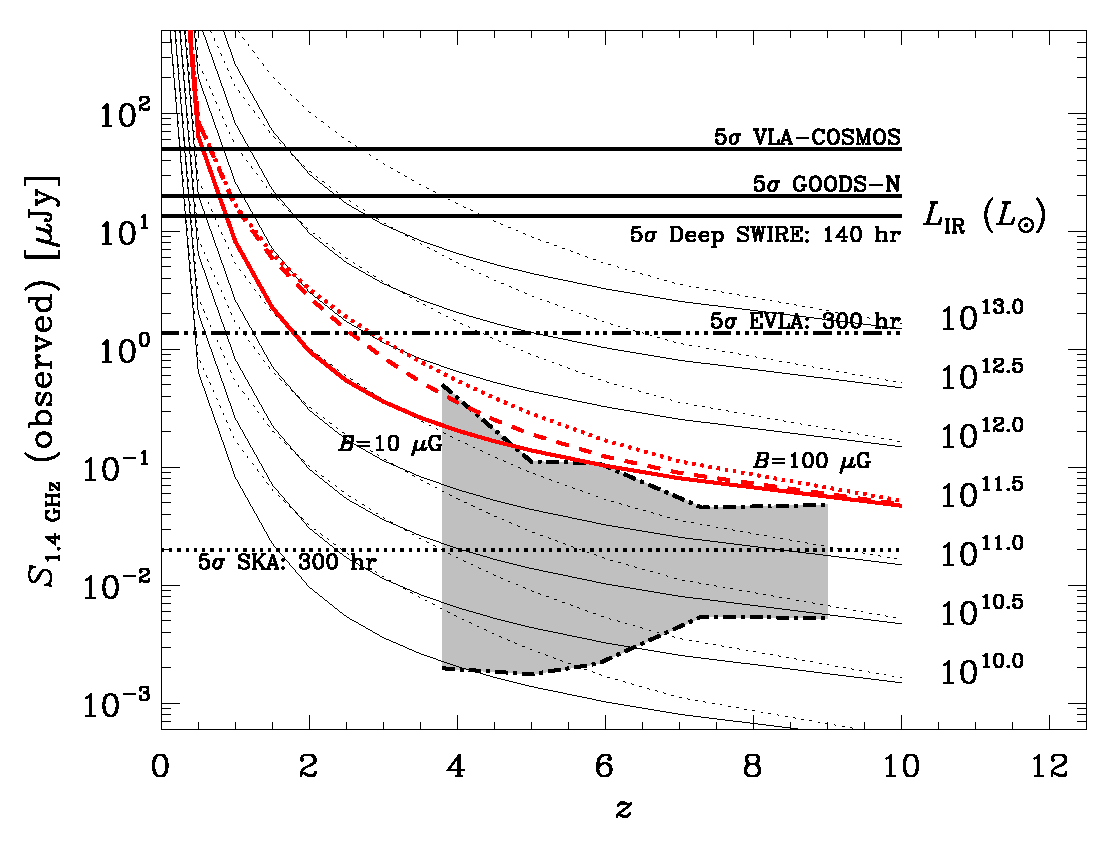
\includegraphics[width=0.8\linewidth]{galaxy/murphy_f3.eps}
\end{center}
\vspace{-0.5cm}
\caption{\citet{2009ApJ...706..482M}より転載。期待される1.4 GHzフラックスを
様々な遠赤外線光度($L_\mathrm{IR}$)の銀河について、赤方偏移の関数として表示したもの。
%
平均的な遠赤外線銀河(LIRG: $L_\mathrm{IR}\sim10^{11.5}$ $L_\odot$、SFR$\sim50$ $M_\odot$ yr$^{-1}$相当)の場合の1.4 GHzフラックスは赤で表している。
%
SEDモデルは、近傍で見られるような電波・遠赤外線相関に基づき、
シンクロトロン放射については、磁場の強度依存性や宇宙背景放射を
逆コンプトン散乱する事による高エネルギー電子のエネルギー減衰
(高赤方偏移で重要)等を
考慮したモデルを用いている。同じ遠赤外線光度について、磁場強度の
異なる場合をプロットしている(実線と点線はそれぞれ10 $\mu$Gと100 $\mu$G;
$L_\mathrm{IR}=10^{11.5}$ $L_\odot$の場合は、破線で磁場強度50 $\mu$Gの場合も
示している)。
又、様々なサーベイ観測の
検出限界も水平線で示されている(式\ref{eq:detection_limit})。灰色に塗られた部分は、
$z\sim 4$--9でのUV光度関数から期待される範囲を示している。
SKAにより初めて、UV (観測される波長では、可視・近赤外線)で
実際に観測されている$z>4$
での銀河種族をサンプル出来る事が判る。また、
$L_\mathrm{IR}=10^{11}$ $L_\odot$といった遠赤外線光度は、ALMAによって観測される
高赤方偏移銀河の典型的限界とも一致する。}
\label{fig:murphy}
\end{figure}

SKAがALMAに対して有利な点は、広い視野である。
ALMAはその視野の狭さから、一般にはサーベイ観測には向かない。
電波で銀河の星形成活動をトレースする意義は、遠赤外線と同様、
ダストによる減光が無視できる点にある。従って、サーベイ観測
という観点からは、SKAはALMAよりも遥かにダスト減光のバイアスの
ない星形成銀河サンプルを得るのに適した望遠鏡であると言える。

積分時間$t_\mathrm{int}$、バンド幅BW、実効的開口面積$A_\mathrm{eff}$、
システム温度$T_\mathrm{sys}$の時、理想的なrmsノイズレベルは
下の様に評価されている\citep{2009ApJ...706..482M}:
\begin{eqnarray}
\left(\frac{\sigma_\mathrm{rms}}{\mathrm{nJy}}\right)\simeq 4
\left(\frac{\mathrm{BW}}{\mathrm{GHz}}\right)^{-1/2}
\left(\frac{t_\mathrm{int}}{300~\mathrm{h}}\right)^{-1/2}
\left(\frac{A_\mathrm{eff}/T_\mathrm{sys}}{15000~\mathrm{m^2~K^{-1}}}\right)^{-1}
\label{eq:detection_limit}
\end{eqnarray}
ここで、$A_\mathrm{eff}/T_\mathrm{sys}=15000~\mathrm{m^2~K^{-1}}$と
BW = 1 GHzは
SKA2で期待される値で、SKA1-MIDでは
$A_\mathrm{eff}/T_\mathrm{sys}=1630~\mathrm{m^2~K^{-1}}$、BW = 770 MHz
である、SKA1-SURVEYでは
$A_\mathrm{eff}/T_\mathrm{sys}=391~\mathrm{m^2~K^{-1}}$、BW = 500 MHzである。

\section{国際SKAのサイエンス}\label{galaxy.s2}

%%%%%%%%%%%%%%%%%%%%%%%%%%%%%%%%%%%%%%%%%%%%%%%%%%%%%%%%%%%%%%%%%%%%%%%%%%
\subsection{水素原子吸収線系で探る銀河進化}
\label{subsec:international_21cm}
%%%%%%%%%%%%%%%%%%%%%%%%%%%%%%%%%%%%%%%%%%%%%%%%%%%%%%%%%%%%%%%%%%%%%%%%%%

国際的にも、クエーサー電波連続光を背景にして、視線方向にある
水素原子21 cm線吸収線を検出することにより、
銀河進化を研究する手法は注目されている。吸収線は輝線に比べて、
明るい背景光を
利用できるという利点があるために、再電離期までの遠方($z\sim 6$)に
わたってサンプルが取られることが期待される。
特に、活動銀河核(AGN)周りのガス-- \textit{associated absorber} (ここでは
「AGNに附随するガス」と呼ぶ)--の
運動をトレースする研究や、
遠方クエーサーの視線上にある中性水素雲-- \textit{intervening absorber}
(ここでは「吸収線系」と呼ぶ)--を
サンプルして銀河進化を調べる研究が挙げられる\citep{morganti14}。
以下に、AGNに附随するガスと吸収線系について、
どのような議論が国際サイエンスブックでなされているかを紹介する。

\paragraph{AGNに附随するガス}

H {\sc i}吸収はAGN周りのガスの物理状態をトレースするのにこれまでにも
使われてきた。例えば、Centaurus Aの電波源を背景にした21 cm吸収線の
検出は1970年に遡り\citep{1970ApJ...161L...9R}、核周辺を取り巻くガス
\citep{2008A&A...485L...5M,2012A&A...546A..22S}や
アウトフロー\citep{2013Sci...341.1082M}の運動が調べられている。
特に、後者の論文で観測された4C12.50のアウトフローは1000 km s$^{-1}$の
高速であり、質量放出率は$16-29$ $M_\odot$ yr$^{-1}$である。
エネルギーに換算すると降着エネルギーの$0.2-0.3\%$がアウトフローに
転換されている事になる。アウトフローばかりでなく、アウトフローのエネルギー源
に当るAGN中心のブラックホールへ降着しているガスの
インフローを捉える試みもなされているが\citep{1989AJ.....97..708V}、
降着円盤成分等との切り分けは容易ではない。

AGNに附随するH {\sc i}ガスに関する、H {\sc i}量、検出成功率、
ガスの運動、天体のタイプとの関係等は、Gerebら\citep{gereb14}に
よってまとめられている。彼らは$z=0.02$から0.23の電波AGNを
サンプルとし、それらの吸収線profileをスタッキングする事でより深い
検出限界に挑んだ。スタックしなくても検出できる
もの($N_\mathrm{HI}\sim 7\times 10^{20}$ cm$^{-2}$)が
あった一方、それ以外の検出できない
ものはスタックしても検出できなかった($N_\mathrm{HI}<2.26\times 10^{19}$ cm$^{-2}$)。
つまり、水素の柱密度に関して二極化の傾向がある事になる。また、コンパクトな
電波源の方が広がったものよりH {\sc i} 21 cm吸収が検出される傾向にあった。
これは、コンパクトな電波源の方がガスを多く持っている傾向がある事を示唆する。

AGNに附随する21 cm吸収は、$z\geq 0.1$では40天体、$z\geq 2$では僅か2天体で
ある\citep{1991PhRvL..67.3328U,1999ApJ...510L..87M}。高赤方偏移での検出が
少ないのは、高赤方偏移では可視域で明るいAGNに観測がバイアスしており、そのような
明るいAGNは周囲のガスを電離してしまうからであろうと考えられる\citep{2012ApJ...759..117C}。
SKAでは、暗い天体まで観測する事によって、バイアスは改善する事が期待される。
特に、SKAは広い視野を持つため、
サーベイ効率がいいので、ブラインドサーベイを実行できることからも、上記のバイアスは
低減されることが期待される。実際、SKA1では、およそ$z\sim 3$にまで届く感度が実現
される。SKAの前にも、ASKAPによって$z\sim 1$に近い所まで迫る事ができると
期待されている。

\paragraph{吸収線系}
遠方にある明るい電波源を使う事により、その手前にあるH {\sc i}雲の
21 cm吸収を検出する研究を行う事が出来る。そのような雲を21 cm吸収線系と
呼ぶ。これまでの21 cm吸収線系のサンプルは、ほぼ全てがLy$\alpha$の
吸収線系として知られているものをターゲットとして得られたものである。
それられの天体は、地上からLy$\alpha$が観測できる赤方偏移($z>2$)が対象となり、
ダスト減光の大きな雲はサンプルから漏れる傾向にある。SKAでは、
このバイアスを克服するために、連続光源自体を電波で探査し、これまでの
可視望遠鏡で得られていたサンプルとは独立のサンプルを取る事が
求められる。
SKA1では、$z\sim 3$まではSKA1-MIDもしくはSKA1-SURVEYで
$z$が3よりずっと大きなところはSKA1-LOWで観測できる。
SKA2では、21 cm吸収線系のブラインドサーベイが$z\sim 6$かそれを超える
赤方偏移まで可能であると見積られている\citep{2004NewAR..48.1259K}。

遠方銀河の中性水素に関して、過去10年の世界における研究の進展は
主として以下のようになる。
\begin{enumerate}
\item 電波CO輝線による分子ガスの観測は、近年のsubmm、mm波
干渉計の感度向上に伴って、遠方銀河まで出来るようになって来た。
近年の観測によれば、銀河の分子ガス量は、中性水素ガス量に比べて
概して$0<z<2$で急速に進化しているという結果が
ある\citep{2011MNRAS.418.1649L} (図\ref{fig:lagos})。しかし、
個々の銀河についてそれぞれ分子ガスと中性水素ガスの比を詳しく
観測する事はまだ出来ていない。これはALMAとSKAとの共同観測に
よって達成する事が期待される、SKA時代の新課題である。
準解析的モデル等によるモデル化も進みつつある\citep{2011MNRAS.418.1649L}
(図\ref{fig:lagos})。
\item DLAの21 cm線によるフォローアップ観測では、実は多くが
21 cmでは吸収されていない。この解釈は、大部分のDLAは、
スピン温度1000 K程度以上である事が分かっている\citep{2014MNRAS.438.2131K}。
(21 cm光学的厚さ$\tau$は、スピン温度の逆数に比例する事に注意。)
\end{enumerate}

SKA以前にも、以下のようなpathfinderによる観測が計画されている。
ASKAPによるFLASH(the First Large Absorption Survey in
H {\sc i})\footnote{http://www.caastro.org/research/evolving/flash}サーベイは南半天球全体の明るい($>$50 mJy)電波
連続光源(電波銀河とクエーサー) 150,000個の視線方向に
ある21 cm吸収線系を$0.5<z<1$の
範囲で探査する。この探査では、視野当り
2時間の積分時間で、1 Jyの背景光源に対して$\tau\sim 0.01$の
光学的厚さが5 $\sigma$で検出でき、
最も暗い(50 mJy)の光源に対しては$\tau\sim 0.3$である。
ApertifとMEERKATによるサーベイでは、より小さい天域に絞って
より深い観測を行う事が計画されている。

\begin{figure}[tbp]
\begin{center}
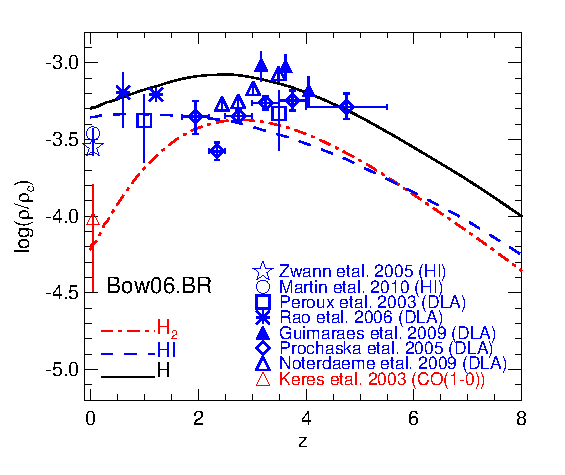
\includegraphics[width=0.7\linewidth]{galaxy/lagos_HI_H2a.eps}
\end{center}
\vspace{-1cm}
\caption{論文\citep{2011MNRAS.418.1649L}より転載。
準解析的モデルから予想される全ての電離していない
水素(実線)、水素原子(破線)、水素分子(鎖線)の
宇宙全体での密度を宇宙の臨界密度で規格化したもの
の赤方偏移進化。観測データは青($z=0$の三角以外)は
水素原子、赤($z=0$の三角)は水素分子の観測をプロット
している。}
\label{fig:lagos}
\end{figure}

SKA1で提案されている10,000平方度のサーベイを行うと、
30 mJy程度の明るさの背景光源に関しては
5 $\sigma$の検出限界で$\tau\sim 0.015$程度のものまで観測できる
(10 mJyの背景光源では$\tau\sim 0.05$、2--3 mJyのものでは
$\tau\sim 0.1$)。全部で数千個規模の21 cm吸収線系のサンプルが
$z=3$程度にまでわたって得られると期待される。

\subsection{電波再結合線で探る冷たい中性水素雲}

水素21 cm線だけが中性(電離度が低い)雲を見る電波のトレーサーではない。
電波($<350$ MHz)での炭素や水素の電波再結合線を観測する事で、
冷たい中性雲をトレースする可能性も検討されている\citep{oonk14}。
冷たい中性雲は、宇宙線によって少し電離しており、その電波再結合線を
捉えるのである。それにより、冷たい中性ガス
(CNM)の温度、電離度、
炭素の存在比等が分かる。\ref{subsec:international_21cm}節で述べた
中性水素21 cm線だけでは区別できないcold、warmの二相を、電波再結合線
がcoldのみで検出できる事を使うと区別できる。

Low Frequency Array (LOFAR)で、系外電波源Cygnus A (Cyg A)を
背景光として、電波再結合線を吸収線で検出した最初の例が
図\ref{fig:oonk}に示されている。ただし、再結合線自体は
銀河系の中性ガスに由来するものが検出されている。
電子温度110 Kと電子数密度
0.06 cm$^{-3}$が観測から導かれている。Cygnus Aに附随する
H {\sc i}ガスの光学的厚さは、4 km s$^{-1}$の速度分解能で
3 $\sigma$の上限$\tau_\mathrm{HI}^{3\sigma\text{upper}}=1.5\times 10^{-4}$が得られている。SKAでは系外の
中性ガスの吸収を遠方の電波源を用いて観測できることが
期待される。

銀河系の電波再結合線の観測も当然
SKAで推進できる\citep{oonk14}が、ここでは系外銀河の
観測に焦点を絞る。最近、LOFARにより、系外銀河M82の炭素電波再結合線が
検出された。これは、電波再結合線が冷たい中性水素ガスのトレーサーとして
観測的に使える可能性を拓くものである。

電波銀河を背景光源として用いることにより、SKAでは電波再結合線を吸収線で
$z=0$から5にわたって検出できると期待される。LOFARでも比較的近傍の数百個程度
の電波銀河を背景光源として使う事ができるが、SKA1-LOWでは$10^5$個程度にまで
増えると期待される\citep{oonk14}。同一の吸収天体による複数の電波再結合線を
同定する事で、その天体の赤方偏移も割出す事が出来る。
また、近傍銀河なら、それ自体の電波放射を背景光源とした電波再結合線も
検出できる。SKA1-LOWでは500個程度の近傍星形成銀河が電波再結合線で
観測できると期待されている(SKA2では3000個程度)。

\begin{figure}[tbp]
\begin{center}
\includegraphics[width=0.6\linewidth,angle=90]{galaxy/oonk_rrl.eps}
\end{center}
\caption{論文\citep{2014MNRAS.437.3506O}より転載。
銀河系の電波再結合線を系外電波源を背景にして検出した最初の
例。LOFARによる。33--57 MHzにある48個の炭素$\alpha$線を
スタッキングし、得られたスペクトル。
黒い実線はデータ、赤い破線はガウシアンでフィットした
結果。}
\label{fig:oonk}
\end{figure}



%%%%%%%%%%%%%%%%%%%%%%%%%%%%%%%%%%%%%%%%%%%%%%%%%%%%%%%%%%%%%%%%%%%%%%%%%%
\subsection{電波連続波で探る銀河進化}
\label{subsec:international_cont}
%%%%%%%%%%%%%%%%%%%%%%%%%%%%%%%%%%%%%%%%%%%%%%%%%%%%%%%%%%%%%%%%%%%%%%%%%%

\ref{galaxy.s1}節で述べた様に、銀河の電波連続波の光度は星形成率の
良い指標である。特に、紫外・可視域の星形成率指標(紫外連続光光度、
バルマー系列輝線光度等)に比べると
ダスト減光の影響がないという利点がある。また、ダストの赤外放射光度も
星形成率の良い指標であることが知られて
いる\citep[e.g., ][]{1998ARA&A..36..189K,2000PASJ...52..539I}が、ダストが極端に
少ない環境では星形成活動指標として使えないことが予想
される\citep{2001A&A...366...83H}。一方で、
電波連続波はダストのない環境でも星形成率指標として利用できる点で
ダストの影響を受けない星形成活動指標と言える。

\color{red}
また、電波連続線によるサーベイでは活動銀河核(AGN)の一種である電波銀河が明るい側で卓越した成分として現れるという特徴がある。電波銀河は、銀河中心の超巨大ブラックホール(SMBH)からの高エネルギージェット及びMpcスケールの巨大なローブから放射される強力なシンクロトロン放射が特徴的である。この放射強度は典型的に星形成銀河の100倍程度であるため、通常の星形成活動起源の電波放射とは分離される。電波銀河は降着の最終期また、inter cluster medium (ICM)への物質輸送も行われる。そのため、AGNはSMBHへの物質降着に起因する減少であるため、電波銀河の電波放射の赤方偏移進化を探ることで銀河-ブラックホール共進化が銀河進化に果たしてきた役割の示唆を得ることができる。
\color{black}

ここでは国際サイエンスブックの
\citet{murphy15}に基づき、SKAへ向けて国際的にどのような
観測が検討されているかを紹介する。彼らは特に、ultra-deep SKA1-MID/Band 5
reference survey \citep{prandoni15}に着目している。Band 5の周波数域は
4.6--13.8 GHzである。

従来、電波域の銀河サーベイの周波数は低周波、特に1.4 GHzでの
サーベイが、視野(primary beam)が大きい点とシンクロトロン放射強度が
周波数に対して負冪の依存性を持っている(つまり、低周波になると
銀河が明るくなる)点で有利であったので、主流であった。
例えば、\citet{2008MNRAS.386.1695S}
では、Multi-Element Radio-LInked Network (MERLIN)とJansky Very Large Array (JVLA)の
1.4 GHzの観測とJVLAの4.8 GHzの観測を用いて、$z<3$での宇宙の星形成史を
導き、可視域等で得られたものと整合的な値が
得られた(\citealt{2010ApJS..188..178M}も参照)。また、
\citet{2009ApJ...690..610S}
では、JVLA 1.4 GHzの観測により、$z=1.3$までの電波連続波光度関数の進化を
観測的に明らかにした。ただし、感度の関係から光度関数の高光度側に
基づいて議論が構築されている。

\color{red}
さらに近年では、COSMOS領域においてJVLAを用いて3GHzにおけるさらに深い($F_{\rm lim}=11.7 {\rm \ \mu Jy}$)サーベイ(VLA-COSMOS 3GHz Large Project)が行われた\cite{2017A&A....602...A1}。
このサーベイに基づいて、星形成銀河とAGNについて$z \leq 6$における電波光度関数の進化モデルが構築された\citep[e.g., ][]{2017A&A....602...A6, 2017A&A....602...A5, 2018A&A....614...47N}。
特に、星形成銀河については紫外線や赤外線といった他の星形成指標から得られた星形成史との比較がなされており、銀河形成期から現在に至るまでこれらの波長帯と整合的な結果が得られる事が確認されている。ただし、感度による制限から星形成銀河電波光度関数の暗い側についての傾きは依然として定められていない。
銀河中の星形成は宇宙再電離の主要因であると考えられている\citep[e.g., ][]{2016MNRAS....463...1968Y}ため、高い感度の観測によって光度関数の暗い側のパラメータについてより厳しい制限が付けられることが今後求められる。
また、電波銀河と異なり、母銀河からの熱的放射が電波放射の大半を占めるAGNの種族であるRadio-Quiet AGN (RQ AGN)についても、電波帯における暗さから進化を議論している研究は少ない\citep[e.g., ][]{2011ApJ...740...20P, 2015MNRAS...452...1263P}ため、SKAによる更新が期待される。
SKA1では0.12GHz (SKA1-low)においてVLA-COSMOSと同程度の感度である$20\ {\rm \mu Jy}$におけるAll-skyサーベイ、1GHz (MID Band 1 and/or 2)において$F_{\rm lim}=50 {\rm \ nJy}$の感度による$1 {\rm deg}^2$にわたるUltra-deepサーベイなどが計画されている\cite{prandoni15}ため、銀河形成・進化についてより詳細な描像が得られると考えられる。
また、電波連続波による銀河計数についての近年の理論的な研究には\cite{2017ApJ....842...95}, \cite{2017MNRAS...469...4083S}が挙げられる。特に、\cite{2017ApJ....842...95}では銀河の星形成活動がSMBHによるフィードバックによって抑制されるまでの各物理過程のタイムスケールを評価することで、銀河種族ごとの赤方偏移分布について解析的なモデル構築を行っている。
ここでも、SKAによる低振動数電波観測によって検出される銀河計数の評価を行っている。
\color{black}


\citet{murphy15}がSKAで着目しているサーベイは比較的高周波に着目している点に特徴がある。
SKAではその高感度から、$\gtrsim 10$ GHzでも、従来の
電波望遠鏡に比べると格段に高いサーベイ効率で
銀河サーベイを行う事ができる。Band 5では、SKA1-MID、SKA2では
それぞれ1平方度当り約30、85個の銀河が検出できると見積られる。
10 GHzもしくはそれ以上の高周波は、
以下の2点で科学的利点がある: (i)
より高い角分解能で観測できる。特に、200 kmのベースラインが取れれば、
10 GHz以上の周波数での観測は、各分解能0.03秒角以下を達成でき、
これは則ち、$z\gtrsim 1$にある銀河でも250 pcスケールが分解できる事を
意味する。また、この分解能は、可視・近赤外域で計画されている\textit{JWST}等
の分解能とも良くマッチしている。(ii) 高周波で卓越するfree--free放射は、
低周波で卓越するシンクロトロン放射に比べて、大質量星からの
電離光子放射光度を直接的に反映する点で現在の星形成活動を
良くトレースしている。特に高赤方偏移では、
シンクロトロン放射を担う高エネルギー電子は、
宇宙背景放射を逆コンプトン散乱してエネルギーを失う傾向にあるので、
シンクロトロン放射は星形成活動のトレーサーとして使えない可能性がある。
これらの二点に基づき、彼らはSKAでの10 GHz以上の周波数域を
強く要求している。特に、
30 GHzまで周波数域を拡張することにより、ALMAと
周波長が連続的に取れる面でも、科学的メリットが大きいと主張する。

特に、free--free放射の重要性は、若いスターバースト\color{red}銀河\color{black}で顕著になる。
近傍の若いスターバーストの電波スペクトルは、
free--free\color{red}放射\color{black}が卓越していると解釈できるフラットな周波数依存性を持つという
結果が得られている\citep{1993ApJ...410..626D,2003ApJ...593..733R,2005A&A...436..837H}。
電波スペクトルの年齢依存性は、高赤方偏移ではとりわけまだ定まった結論を得るに
至っていない: 遠方のスターバースト\color{red}銀河\color{black}のいくつかはフラットな電波
連続波スペクトルを
持つ\citep{2005A&A...436..837H,2006A&A...460...67H,2011MNRAS.415.3473V}のに
対し、反対の傾向を持つ遠方銀河も
ある\citep{2011MNRAS.410.1155B,2014MNRAS.442..577T}。
広帯域を持つSKAでは、電波スペクトルの形(特にspectral index)を
様々な赤方偏移で決めるのに適しているので、電波連続波スペクトルの
年齢(もしくは赤方偏移)に依る進化を明らかにするのに適している。
特に、10 GHz以上の周波数域が観測できる事が理想的である。

シンクロトロン放射自体も、超新星等に伴う星間空間での高エネルギー過程を
トレースする重要性があるので、理解を欠かす事はできない。また、
星間磁場の強さや進化に対する制限も得られる可能性があり、free--free\color{red}放射\color{black}成分に
勝るとも劣らず重要である事も強調しておかねばならない。
シンクロトロン\color{red}放射\color{black}とfree--free\color{red}放射\color{black}の両方を観測できるSKAの広帯域は、
この点でも魅力的である。

最後に、連続波以外にも、
30 GHzまで周波数域を拡張する利点は幾つかある。
表\ref{tab:summary_line}ではバンドの上限周波数は
10 GHzを仮定したが、30 GHzまで拡張されれば、AGNのH$_2$Oメーザーの
観測が近傍銀河でも
可能になる。また、CO ($J=$ 1--0)も$z>2.8$で
観測可能となる。つまり、重要な輝線の観測範囲が低赤方偏移へ
降りてくる。ALMAとシームレスに繋がる点も再度強調しておく。


\section{日本が狙うサイエンス}\label{galaxy.s3}

系外銀河の観測や銀河進化の研究に於ける日本の強みは、
観測的には、これまで野辺山等の観測で培って来た
電波観測の知識と経験の蓄積である。特に、
ALMAの観測時間へのアクセスがあることが実際的に
有利である。
ALMAはダストと多彩な分子を観測するのに適しており、
SKAの水素原子の観測と組み合わせることによって、
原子ガスから、分子ガスを介して、星形成と重元素汚染が
起きる、いわゆる星間ガスのリサイクルの全貌を捉える事が
できるのである。理論的にも、日本は銀河形成のシミュレーションと
銀河の化学進化モデルが強く、理論的予言は言うまでもなく、
SKAやALMAによってより暗い銀河、
より遠い銀河が見えて来た時に、その理論的解釈をいち早く提供できる
利点がある。

銀河形成研究においては、主として3つの赤方偏移の範囲が重要である。
まずは宇宙初期、ガスから星が形成されることによって銀河が成長していく、
いわば銀河の成長期($z > 3$)である。
特に星形成の前夜ともいえる、大量のガスを持った進化初期の銀河の
直接観測は銀河形成の物理の検証として本質的に重要である。
そして、階層的構造形成により銀河が銀河としてのグローバルな性質を持つように
なってゆき、ハッブル分類のような銀河の形態が出現する時代($1 < z < 2$)が
銀河進化の文脈で極めて興味深い。
この時代は銀河の合体率(merging rate)、平均的な星形成率や
ダストで隠された星軽視の割合がピークを迎える(\S~\ref{galaxy.s0.5}参照)
銀河進化の激動の時期であり、様々な物理過程が複雑に絡み合って
統一的な見解が得られるには遠く至っていない。

そして、銀河進化研究において最近とみに見落とされがちなのが$z=0$、すなわち
近傍宇宙である。
銀河進化全てに関わる過程は、「ゼロ点」である近傍宇宙の素過程と比較されて初めて
「進化」を追ったと言える。
これは全く自明なことであるが、どういうわけか最近の銀河進化研究においては研究の主流から
外れた分野と見なされる傾向があった。
また、近傍宇宙の銀河の物理の詳細を突き詰めることで星間物理とのクロスオーバーを
構築することができ、星間物理--近傍銀河--遠方銀河という道筋を一つの大きな
流れとして扱うことができるようになる。
気取った言い方をすれば、星間物理から銀河進化研究の``シルクロード''を繋いでゆく研究が
近傍銀河の物理である。
ここでは上記の日本の強みに鑑み、いくつかのサイエンス
ケースに対してどのような貢献ができるのかを、3つの代表的時期に関連して
紹介する。

\subsection{近傍銀河: 星間物質の性質$\cdot$進化、星形成の統一的理解}

ここではまず、$\sim 10\;\mbox{Mpc}$程度の距離にある近傍銀河の詳細なSKA観測にもとづく日本が
狙うべきサイエンスについて述べる。
特に、1) 最近明らかになってきた原子ガスと分子ガスの遷移層にあるdark gasの正体の解明、2)
低金属量環境下における原子ガスからの星形成、の2点について以下で述べる。
ここでの議論はSKA-JP星間物理サブグループとのシナジー研究となっている。

これまで、21~cm輝線は光学的に薄いという仮定のもと原子ガスの質量が見積もられてきた。
しかし\citet{2015ApJ...798....6F}は、Planckによる天の川銀河の詳細なダスト分布と{\sc H\,i}データの比較から、
21~cm輝線放射の50\%程度は冷たく、光学的に厚い水素原子からのものであることを示した。
この研究において、光学的に厚い水素原子こそが、21~cm輝線やCO輝線で感度のない
密度範囲$100\mbox{--}1000 \; \mbox{cm}^{-3}$のガス(dark gas)の正体である可能性を示唆している。
今後はdark gasを含む、銀河ISM進化の統一的理解のために、電離ガス・原子ガス・分子ガスの量・分布・運動状態などを銀河内・異なる銀河間で網羅的に比較することが重要である。
天の川銀河は最も詳細に調べることのできる銀河であるが、我々がその中に存在しているために、銀河の構造とISMの性質の比較をすることは容易ではない。
円盤銀河における渦状腕や棒状構造などの銀河スケールの大規模な構造は、銀河ISMの物理状態に大きな影響を与える。
今後、SKAで達成される角度分解能($\sim 0.1\; \mbox{arcsec}$)によって、2本の卓越した渦状腕を
持つ(grand-design)渦巻銀河が存在する典型的な距離10~Mpcでも5~pcの空間分解能を達成することができる。
ALMAで取得可能な近傍銀河における詳細なダスト・分子ガス分布と、SKAで取得される詳細な原子ガス分布との比較は日本が狙うべき重要なテーマの一つである。


上で述べた力学的な擾乱だけでなく、ダスト量に比例していると考えられる金属量の違いも、銀河ISMの物理状態に
影響を与える。
近年の星形成に関する理論研究において、ISMが分子ガスの状態であることは星形成の必要十分条件ではなく、低金属量な環境下では原子ガスからも星形成をする可能性が示唆されている。
矮小銀河や円盤銀河外縁部などの近傍の低金属量環境下での原子ガスの性質の詳細な理解もまた、SKAで行うべきサイエンスの一つである。
以下では、この分野についてわかりやすく、簡潔にレビューしている\citet{krumholtz2013}をもとに、
水素原子--水素分子間の遷移と星形成に関して紹介する。

原子ガスは分子ガスの原材料と考えられているが、近傍銀河における星形成率は、分子ガスとの相関はいいものの、原子ガスとの相関はそこまでよくない
\citep{2002ApJ...569..157W, kennicutt2007, 2008AJ....136.2846B, 2008AJ....136.2782L}。
なお、分子ガス質量を星形成率で割ったdepletion time scale $t_{\rm dep}$は、近傍円盤銀河ではほぼ一定であり、2~Gyr程度であることも観測的に示されている\citep{bigiel2011}

星間水素の化学状態(原子ガスないし分子ガス)を決めているのは、Lyman-WernerバンドのUV光による
水素分子の解離と、(金属量が太陽の十万分の1程度以上ならばダスト上での水素分子形成のバランスである
\citep{omukai2010}。
太陽近傍の典型的なUVの輻射強度における水素分子の乖離率は、水素分子一つあたり$5\times 
10^{-11}\, \mbox{s}^{-1}$ \citep{1996ApJ...468..269D}であるのに対し、太陽金属量(ダスト量が金属量に
比例すると仮定\footnote{これは化学進化がある程度以上進んだ銀河ではよい近似であり、近傍銀河では
問題なく使える。低金属量銀河の場合についてはこの仮定は破れる。詳細は星間物理の章を参照。})、
水素原子の柱密度$100
\; \mbox{cm}^{-3}$における水素分子の形成率は、水素原子一つあたり$3 \times 10^{-15}\; \mbox{s}^{-1}$である。
そのため、分子解離率と分子の形成率のバランスから予想される太陽近傍における水素分子の割合は非常に
低く$10^{-4}$となってしまう。
しかし、ダストの豊富な領域ではLyman--WernerバンドのUV光子が十分に遮蔽され、水素分子の割合が1になり、分子雲が形成されると考えられる。
そのため、分子雲の典型的な構造としては、UV光の減光があまり効かない水素原子が優勢な外層、UV光の減光が効き始め水素分子が優勢な内側、という状態が期待される
\citep[e.g.,][]{van_dishoeck1986, sternberg1988, neufeld1996, liszt2002, glover2007, 2008ApJ...689..865K, 2009ApJ...697...55G, 2010ApJ...709..308M, mac_low2012}。

分子ガス--星形成率間のよい相関の理由としては、星間水素ガスの化学状態と熱状態(温度)を決めているのが、両方ともダストによる遮蔽である点が挙げられる。
まず、化学状態に関しては、(ダストによる吸収を受けつつの)Lyman--WernerバンドのUV光子による水素分子の光乖離、ダスト粒子上での水素分子形成のバランス、熱状態に関しては、やはりLyman--WernerバンドUV光子によるダストの光電効果加熱とダスト--ガス間の熱交換、衝突励起されたガスの輝線放射による冷却のバランスで決まっている。
そのため、星間水素の化学的プロセスと熱的プロセスの、ガスの体積密度、柱密度、UV輻射場強度への依存性は極めて似ている。
輝線放射による冷却と水素分子形成は両方とも、衝突によるものであり、冷却率と形成率は両者とも、密度と金属量に$n^2 Z’$という依存性を持つ。
光解離と光電効果加熱は両者とも、UV輻射場強度とダスト減光とに同じ形で依存している。

この類似性により、ガスの温度や化学状態は、幅広いガス密度、ダスト減光、金属量範囲で相関がよい。
原子ガスから分子ガスへの遷移はだいたい$>100\; \mbox{K}$から$\mbox 10\;  \mbox{K}$のところでおきるが、
これを決めているのはダストによる遮蔽である:
星間水素の大半が水素分子であるような遮蔽の効いている領域では、低温になっており、逆に遮蔽の効いていない場所では、加熱率が高いために高温となっている。
そのため、水素分子と星形成の間にはよい相関がある:
水素原子から水素分子への変換が星形成を引き起こしているわけではないが、ガス温度の低下は水素原子と水素分子間の遷移が付随するのである。

低金属量環境下では、完全な水素原子から完全に水素分子になるためのタイムスケールは力学的時間と同程度であり、熱的平衡状態になるのに必要なタイムスケールは1/1000程度と短い。
化学的タイムスケールと熱的タイムスケールは両者とも金属量に依存し、低金属量環境化では長くなる。
一方、星形成雲の力学的時間(星形成のタイムスケール)は金属量に依存しない。
そのため、$熱的タイムスケール < 力学的タイムスケール < 化学的タイムスケール$となる金属量があるはずである。
このことは、星形成を支配しているのが化学状態でなく熱状態であるとすれば、星間水素が水素分子になる前に星形成が起こるということを示している。
そのような状況下では、星形成率は水素分子ではなく水素原子と相関がよくなるはずである。
\citet{glover2012}は数値シミュレーションを行い、水素原子からの星形成の可能性を示し、\citet{krumholtz2012}は
解析的モデルをたて、太陽の金属量の1--10~\%でこの効果が見られる可能性を示した。

SKA-JP銀河進化サブグループは、ALMAとの実践的リンクという強みを生かし、近傍の様々な
金属量、進化段階の銀河について、空間的に分解した原子--分子転移を追求し、遠方銀河と
比較されるべき基準となる物理過程を明らかにすることを目指す。

\subsection{ガス、ダスト及び星形成を結ぶ拡張スケーリング則の探索と理論化}

銀河の本体が十分に形成されると、銀河の持つ諸量の間に密接な関係が出現する。
これがスケーリング則と呼ばれているもので、銀河進化研究の重要なツールとなっている。
スケーリング則のもっともよく知られている例が、\S\ref{sec:TF}において述べたTF関係、
BTF関係である。
そして銀河にはこれ以外にも様々なスケーリング則が知られている。
ところが、そのほとんどはスケーリングが成立する物理的理由が知られていない
経験的関係式である。
ここでは銀河進化と関連の深いスケーリング則を紹介し、その有機的統合と理論化への大まかな道筋について
述べる。

銀河進化の観点からは星形成率が最も興味ある物理量であり、星形成率の関係する
スケーリング則を検証したい。
2015年現在、銀河の星形成に関係するスケーリング則で最も注目されているのが
星形成銀河主系列と呼ばれる関係である。
これは銀河の星形成率(SFR)と星質量($M_*$)の間に成立する線型関係である。
歴史的に色--等級関係(color--magnitude relation)として知られている経験則と
等価であるが、銀河のカラーではなくSFRおよび$M_*$というより物理的な量を用いた
ことで、星形成率の従うスケーリングが鮮明に浮かび上がってきたのである\citep[e.g.,][]{schiminovich2007}。
どちらも銀河全体について積分量であるので、その間に自明なスケーリング則が存在
することは驚くに値しない。
注目すべきはその傾きが1よりも小さい、つまり大きな銀河ほど単位星質量当たりのSFRが
小さくなっていることである。
このことはSFRの代わりに比星形成率$\mbox{SSFR} = \mbox{SFR} / M_*$を
用いるとより鮮明に見えてくる(図~\ref{fig:sf_ms})
この傾向はダウンサイジングと呼ばれており、1980年代後半から認識されていたものの、その
物理的な意味は現在に至るまで明らかになっていない。

\begin{figure}[thbp]
\begin{center}
\includegraphics[width=0.5\linewidth]{galaxy/schiminovich2007.eps}
\end{center}
\vspace{-0.3cm}
\caption{{\sl GALEX}による紫外線観測で得られた星形成銀河主系列。上の線が
星形成主系列で、下の線は赤い、星形成を停止しつつある銀河(red sequence)に対応する
\citep[][より改変]{schiminovich2007}。}
\label{fig:sf_ms}
\end{figure}


高光度赤外銀河など爆発的な星形成をしている銀河は星形成銀河主系列に乗らず、
1桁以上主系列から上に分布することが知られている\citep[e.g.,][]{buat2005, buat2007}。
これは、星形成主系列が永年的進化をする銀河の道筋であるか、あるいは単に滞在時間の
長い系列であるということを意味している。
また、楕円銀河など星形成をほぼ停止した銀河は主系列から下方に外れ、$\mbox{SFR} = 0$に
至ると図上に乗らなくなる。
このことから、星形成銀河主系列を進化のトラックとして捉えるためには、様々な
側面からの研究が必要であることが分かる。
\citet{genzel2012}は星形成主系列の銀河の分子ガス量の検証を試みた。
銀河サンプルの赤方偏移は$0 < z < 2$であるが、まだケーススタディを集めている状態で、
系統的探査のレベルには至っていない。
\citet{magnelli2012}および\citet{magnelli2014}は星形成銀河主系列における
ダスト温度と分子ガス温度の関連性を研究している。
また\citet{magnelli2015}は、広く知られている銀河の赤外線--電波強度相関と
星形成主系列との関連に注目している。
しかし、中性ガスの観測が$z < 0.5$程度に限られる現在、銀河進化を視野に置いた
研究は難しい。
そして、次に述べる星形成のもう一つの重要なスケーリング則であるKennicutt--Schmidt則と
星形成銀河主系列との関係を明らかにするためには、銀河を空間分解して観測することが
不可欠となる\citep{teruya2014}。
このように、星形成銀河主系列が出現する理由を星間物理的に解明する研究はALMAを経て
SKAに至る観測によって初めて可能になる。

\begin{figure}[htb]
\begin{center}
\includegraphics[width=0.5\linewidth]{galaxy/KS_relation.eps}
\end{center}
\caption{Kennicutt--Schmidt則。ガス面密度$\Sigma_{\rm gas}$、SFR面密度$\Sigma_{\rm SFR}$とも
7桁近い範囲で成立する単一冪型の関係である\citep[][]{kennicutt2012}。}
\label{fig:ks}
\end{figure}

銀河における星形成の物理は比較的局所的な物理条件が関係する現象である。
ところが、古くから銀河の大域的性質と星形成が関係することが知られている\citep[e.g.,][]{roberts1994,kennicutt2012}。
銀河の渦状腕や分子雲、電離水素領域といった局所的な現象と、銀河の形態や全質量などの
大域的な性質が見事に関連している理由はまったく自明のものではなく、天体物理学によって
解明されるべき重要な課題である。
局所的から大域的な様々なスケールで現れる銀河のガス(面)密度と星形成率の関係が
Kennicutt--Schmidt(KS)則である\citep[レビューとしてはたとえば][]{kennicutt2012}。
定量的にはKS則は以下のように表現される。
\begin{equation}\label{eq:ks}
  \Sigma_{\rm SFR} \propto \Sigma_{\rm gas}^n \;. 
\end{equation}
これは、ガス面密度$\Sigma_{\rm gas}$、SFR面密度$\Sigma_{\rm SFR}$ともに7桁近い
範囲で成立する単一冪型の関係である(図~\ref{fig:ks})。
ここで、係数$n$は観測的に$1 < n < 2$の範囲に入ることが知られている。
この係数が1に近いか2に近いかによって、星形成のもととなる分子ガスの物理過程について
異なったシナリオを与える\citep[e.g.,][]{momose2013}。
また、KS則は銀河の化学進化理論においては星形成史を決定する重要な構成要素であり、
銀河進化理論へのインパクトも大きい。
このように、KS則は星間物理から銀河物理にわたる多くの研究者の
興味の対象となっている。

しかし、根本的な問題として、KS則も観測から得られた純粋な経験則であることを指摘
しておかねばならない。
しかも、観測から決まる冪指数$n$についても現在議論が収束していない。
分子雲の重力崩壊や分子雲衝突などの星間過程から理論的にKS関係を求めるには、
まず十分な数の銀河サンプルから目指すべき経験則を
なるべく小さな誤差で示す必要がある。
このために、分子ガス、中性水素ガスともに十分な数があり、共通の選択基準に基づく
銀河サンプルが不可欠となる。
SKAはここにおいて他の追随を許さない重要な役割を果たす。
SKAによって得られたH\,{\sc i}セレクトの銀河サンプルを用い、空間分解されたKS則を$z \sim 1$まで
検証し、KS則を生む本質的な物理過程が何かを明らかにする。
そして、BTF関係や星形成銀河主系列と統一的に扱うことで、銀河が従う究極のスケーリング則を
見出すことができる。 
さらに、SKA-JP星間物理サブグループとのシナジーにより、この結果を星間物理から第一原理的に導く
ことを試みる。
ここまで来て初めて、銀河進化研究も天体物理学として成熟することになるだろう。



\subsection{水素原子21 cm吸収線系で探る銀河進化}\label{galaxy.s3.ss1}

\ref{sec:DLA}節と\ref{subsec:international_21cm}節で述べた様に、
クエーサー等の明るい連続光源を利用して、その視線上にあるガスを
吸収線で検出する事により、そのガスが附随する銀河および銀河間ガスの構造
の宇宙論的時間スケールでの進化を研究する事ができる。特に、地上の
可視望遠鏡でサンプルできる
水素Ly$\alpha$吸収線系はこれまでにも盛んに研究されてきた。最近は
電波望遠鏡を用い、水素の21 cm吸収を、既にLy$\alpha$で
サンプルされた吸収線系、特に柱密度の大きな%damped Ly$\alpha$雲
DLAをターゲットにして観測する研究も行われている。
電波の連続光源自体を無バイアスにサーベイして、可視サンプルに
依らない電波独自の吸収線サンプルを得る事も国際的にSKAでの
主要な科学目標として提案されている。

吸収線系の物理状態を観測的に明らかにするためには、Ly$\alpha$以外の
吸収線も同定することが重要である。例えば、重元素の吸収線から
求められる重元素の組成比は、銀河進化の
重要な側面である化学進化を特徴づける重要な量である。この
化学進化からの観点からは、日本でも、第一世代星による重元素
合成の痕跡を探る研究\citep{2011ApJ...730L..14K}や世界であまり
注目されていないNa等の重元素に着目して研究した
例\citep{2006ApJ...643..667K}等がある。銀河の化学進化は
日本でも強い分野であり、様々な
元素を横断的に用いて、理論の助けを借りながら、
吸収線系を研究していく事が今後も
期待される。

銀河スケールでの星間ガスのシミュレーションも、日本で
強い分野である。特に、吸収線系と関連する
我々独自の研究として、星間ガスの構造がどれくらい吸収線系の統計に
現れるかを理論的に研究したものがある。
%我々
\citet{2003MNRAS.341L..18H}は、$z\sim 3$で典型的に見られる
星間ガスの構造を見るために、銀河円盤の
シミュレーション\citep{2001ApJ...547..172W}に基づいた
星間ガスの構造を計算した。更に、観測との比較のために、
星間ガスの密度に敏感な
水素分子の存在比(水素分子の水素全体に占める割合)の統計を
シミュレーションされた
星間ガスの構造のもとで調べた。その結果、水素分子は、塊状の構造に
局在化されるので、水素分子の存在比の高い($\gtrsim 10^{-3}$)領域が
ちょうどクエーサーの視線上にくる確率は低い(典型的に10\%程度)。
これは、大部分のDLAで水素分子存在比が$10^{-6}$より小さく、
水素分子存在比が高い($\gtrsim 10^{-3}$) DLAがサンプル数は少ないが
大雑把に10\%程度である観測事実\citep{2003MNRAS.346..209L}を良く説明する。

\ref{sec:DLA}節で述べたように、最近DLAをサンプルとした21 cm線吸収の観測も行われて
いるが、21 cm吸収線はあまり検出されて
いない\citep{2012MNRAS.421..651S,2014MNRAS.438.2131K}。
式(\ref{eq:tau21cm})でも見たように、21 cm線の光学的厚さはガスの
スピン温度に依る。つまり、DLAで観測される小さな光学的厚さは、
温度が高い($\gtrsim 10^3$ K)ガス(warm ISM)を見ているためであると解釈される。
つまり、DLAのホスト天体は、warmガスの占める割合が大きく
coldガスの占める割合が小さいと、21 cm吸収線があまり検出されない観測事実を
うまく説明できる。Cold gasは水素分子存在比も
大きい為、cold gasの占める割合の小さな事は、水素分子の存在比の小さな
DLAが圧倒的多数を占めるという上記の観測結果と整合的である。

%我々
\citet{tee15}は、21 cm光学的厚さの分布を上記の
シミュレーション\citep{2003MNRAS.341L..18H}を基に計算した。
その結果を図\ref{fig:distri_21cm}に示す。
シミュレーションの格子点の統計を取る際に、DLAの
選択基準と同一になるよう、水素の柱密度が$2\times 10^{21}$ cm$^{-2}$
よりも大きくなる所だけを数えた。また、ダスト減光は
重元素率に比例すると仮定し、Znの柱密度が$10^{13.2}$ cm$^{-2}$
より大きな柱密度を持つ格子点は、背景にクエーサーが
あったとしても減光のためにサンプルされない\citep{2005A&A...444..461V}ので、統計から
除外した。また、線幅は典型的なdiffuse星間ガスの速度分散の
値$\Delta v=10$ km s$^{-1}$を仮定した\citep{2009ApJ...695..937B}。

\begin{figure}[thbp]
\begin{center}
\includegraphics[width=0.7\linewidth]{galaxy/Inttau_v3.eps}
\end{center}
\vspace{-0.5cm}
\caption{我々の流体シミュレーションによって予言される、
DLAホスト天体の星間ガスに典型的な21 cm光学的
厚さ($\tau_\mathrm{21~cm}$)の分布関数。実線、点線、破線、
一点鎖線はそれぞれ、重元素率0、0.1、0.3、1 Z$_\odot$を
表す(重元素率が高いほど、ダスト減光によってサンプルから
漏れる高い柱密度のものが増える)。DLAの統計と整合的な
水素の柱密度$N_\text{H}>2\times 10^{21}$ cm$^{-2}$
の格子点のみを取った。線幅$\Delta v=10$ km s$^{-1}$を
仮定し、上下の横軸に
それぞれ$\tau_\mathrm{21~cm}$と$\int\tau_\mathrm{21~cm}\mathrm{d}v$を
示す。ピークは$\tau_\mathrm{21~cm}\sim 0.01$にあり、
21 cm吸収線があまり検出されていない事を良く説明する。
SKAでは、このような小さな$\tau_\mathrm{21~cm}$まで
検出できる事が期待される。ダスト
減光の効果が大きくなるほど、ピークは顕著になる。}
\label{fig:distri_21cm}
\end{figure}

図\ref{fig:distri_21cm}から、$\tau_\mathrm{21~cm}$の分布は、
$\tau_\mathrm{21~cm}\sim 0.01$にピークがある。この小さな
光学的厚さは、DLAで21 cm吸収線が検出されていない事を
良く説明する(観測の典型的な検出限界は大雑把に$\tau_\mathrm{21~cm}\sim 0.02$)。
また、重元素率が大きくなり、ダスト減光による選択効果が
大きくなると、$\tau_\mathrm{21~cm}\sim 0.01$のピークは
より顕著になる。小さな$\tau_\mathrm{21~cm}$の原因は、
ガスの温度が比較的高い($\gtrsim 10^3$ K)ことである。
従って、DLAで21 cmがあまり検出されないのは、
温度の比較的高いISMが大部分の体積を占めている事と、
減光による選択効果との結果である事が分かる。

これから日本からのこの分野への寄与としてどのような事が
考えられるであろうか。先ずは、シミュレーションを精密化する
事である。上記のHirashitaらの
%我々の
シミュレーションは、2次元かつ個々の
銀河の(つまり宇宙論的な初期条件とは直接はリンクさせて
いない)計算であったが、最近は、計算機性能の進歩により、
宇宙論的な構造形成に
高分解能のシミュレーションを実装できるようになってきており、
日本の得意分野の一つで
ある\citep{2013MNRAS.428..718O,2014MNRAS.439.3073Y}。
従って、宇宙論的な銀河統計と星間ガスの構造を両方盛り込んで、
21 cm吸収線系の統計を理論的に予言する事をサイエンスの
柱として据える事で、SKAへ貢献していく事ができる。
また、ダストの効果をシミュレーションに入れる取り組みも
行われている\citep{2014MNRAS.443..522Y}ので、
ダスト減光によるDLAの選択効果が、
自由変数を使って記述するのではなく、理論的に予言できる。
銀河の中でのダストの進化も、日本でも最先端のモデル化が
行われている分野である\citep{2014MNRAS.440..134A}。

光源自体に、高赤方偏移($z>3$)で急激に数が少なくなる
クエーサーではなく、ガンマ線バースト残光を使うアイディアも
示されており、その方面での研究も既に進められて
いる\citep{2007MNRAS.380.1715I}。ガンマ線バースト残光は
明るいので、$z>6$の高赤方偏移までも吸収線観測を開拓できる。
またこのような高赤方偏移であれば、COなどの分子吸収線もSKAで
観測される波長域に入ってくる。
理論だけでなく、観測でも、ASKAPのFLASH
%(the First Large Absorption Survey in H {\sc i})\footnote{http://www.caastro.org/research/evolving/flash}
等へ
参加し、日本が独自の
観測時間を持つALMA等でのDLAの分子ガスフォローアップ
を行うことで寄与できる。
実際に、\ref{subsec:international_21cm}節
(図\ref{fig:lagos})で述べたように、ALMAによるCO観測によって分子ガス量の
宇宙論的進化を明らかにする事は、SKAによって
得られるH {\sc i}ガスと可視望遠鏡で得られる宇宙の星形成の
間を繋ぎ、星形成の全貌を明かにする重要性がある。他にも、
FLASHの観測結果と銀河の水素原子量の進化モデルと直接比較できる
独自のパイプラインを開発し提供する等、理論の強みを活かした観測への
直接寄与も可能である。


\begin{thebibliography}{99}
\addcontentsline{toc}{section}{参考文献}
\markboth{参考文献}{参考文献}
\begin{multicols}{2}{\footnotesize
%% A
\bibitem[Akerman et al.(2005)]{2005A&A...440..499A}
 	Akerman, C. J., Ellison, S. L., Pettini, M., \& Steidel, C. C. 2005, A\&A, 440, 499
\bibitem[Asano et al.(2014)]{2014MNRAS.440..134A}
	Asano, R. S., Takeuchi, T. T., Hirashita, H., \& Nozawa, T. 2014,
	MNRAS, 440, 134
%% B    
\bibitem[Babul \& Rees(1992)]{1992MNRAS.255..346B}
	Babul A. \& Rees M. J., 1992, MNRAS, 255, 346
\bibitem[Bacon et al.(2001)]{2001MNRAS.326...23B}
	Bacon R. et al., 2001, MNRAS, 326, 23
\bibitem[Barnes et al.(2001)]{2001MNRAS.322..486B}
	Barnes J. E. et al., 2001, MNRAS, 322, 486
\bibitem[Barnes(2002)]{2002MNRAS.333..481B}
	Barnes J. E., 2002, MNRAS, 333, 481
\bibitem[Barvainis \& Antonucci(2005)]{2005ApJ...628L..89B}
	Barvainis, R. \& Antonucci, R. 2005, ApJ, 628, L89
\bibitem[Bell \& de Jong(2001)]{2001ApJ...550..212B}
	Bell, E. F. \& de Jong, R. S., 2001, ApJ, 550, 212
\bibitem[Benson et al.(2002)]{2002MNRAS.333..156B}
	Benson A. J., et al., 2002, MNRAS, 333, 156
\bibitem[Begum et al.(2008)]{2008MNRAS.386.1667B}
	Begum A. et al., 2008, MNRAS, 386, 1667
\bibitem[Bigiel et al.(2008)]{2008AJ....136.2846B}
	Bigiel, F. et al., 2008, AJ, 136, 2846
\bibitem[Bigiel et al.(2011)]{bigiel2011}
	Bigiel, F., et al., 2011, ApJ, 730, 13
\bibitem[Bigiel \& Blitz(2012)]{2012ApJ...756..183B}
	Bigiel, F. \& Blitz, L., 2012, ApJ, 756, 183
\bibitem[Blitz \& Rosolowsky(2004)]{2004ApJ...612L..29B}
	Blitz, L. \& Rosolowsky, E., 2004, ApJ, 612, 29
\bibitem[Boselli et al.(2014)]{2014A&A...564..66B}
	Boselli, A. et al., 2002, A\&A, 564 66
\bibitem[Bosma(1981)]{1981AJ.....86.1791B}
	Bosma, A., 1981, AJ, 86, 1791
\bibitem[Bourne et al.(2011)]{2011MNRAS.410.1155B}
    	Bourne, N., Dunne, L., Ivison, R. J., Maddox, S. J., Dickinson, M.,
    	\& Frayer, D. T. 2011, MNRAS, 410, 1155
\bibitem[Braun et al.(2009)]{2009ApJ...695..937B}
   	Braun, R., Thilker ,D. A., Walterbos, R. A. M., \& Corbelli, E. 2009,
   	ApJ, 695, 937
\bibitem[Buat et al.(2005)]{buat2005} 
	Buat, V., Iglesias-P{\'a}ramo, J., Seibert, M., et al.\ 2005, ApJ, 619, L51 
\bibitem[Buat et al.(2007)]{buat2007} 
	Buat, V., Takeuchi, T.~T., Iglesias-P{\'a}ramo, J., et al.\ 2007, ApJS, 173, 404 
\bibitem[Burgarella et al.(2013)]{burgarella2013}
	Burgarella, D., Buat, V., Gruppioni, C., et al.\ 2013, A\&A, 554, AA70 
%% C
\bibitem[Calistro-Rivera et al.(2017)]{2017MNRAS.469.3468C}
	Calistro-Rivera et al., 2017, MNRAS, 469, 3468
\bibitem[Cannon et al.(2011)]{2011ApJ...739L..22C}
	Cannon J. M. et al., 2011, ApJ, 739, 22
\bibitem[Cappellari et al.(2011)]{2011MNRAS.416.1680C}
	Cappellari M. et al., 2011, MNRAS, 416, 1680
\bibitem[Catinella et al.(2010)]{2010MNRAS.403..683C}
	Catinella B. et al., 2010, MNRAS, 403, 683
\bibitem[Catinella et al.(2012a)]{2012MNRAS.420.1959C}
	Catinella B. et al., 2012a, MNRAS, 420, 1959
\bibitem[Catinella et al.(2012b)]{2012A&A...544A..65C}
	Catinella B. et al., 2012b, A\&A, 544, 65
\bibitem[Catinella et al.(2013)]{2013MNRAS.436...34C}
	Catinella B. et al., 2013, MNRAS, 436, 34
\bibitem[Chandra et al.(2010)]{2010ApJ...712L..31C}
   	 Chandra, P., et al.\ 2010, ApJ, 712, L31
\bibitem[Condon(1992)]{1992ARA&A..30..575C}
 	Condon, J. J. 1992, ARA\&A, 30, 575
\bibitem[Cucciati et al.(2012)]{cucciati2012}
	Cucciati, O., Tresse, L., Ilbert, O., et al.\ 2012, A\&A, 539, AA31 
\bibitem[Curran \& Whiting(2012)]{2012ApJ...759..117C}
	Curran, S. J. \& Whiting, M. T. 2012, ApJ, 759, 117
%% D
\bibitem[Dav\'{e} et al.(2011)]{2011MNRAS.415..11D}
	Dav\'{e} R., Oppenheimer B. D. \& Finlator K., 2011, MNRAS, 415, 11
\bibitem[de Blok et al.(2003)]{2003MNRAS.340..657D}
	de Blok W. J. G. et al., 2003, MNRAS, 340, 657
\bibitem[de Blok et al.(2005)]{2005ApJ...634..227D}
	de Blok W. J. G., 2005, ApJ, 634, 227
\bibitem[Deeg et al.(1993)]{1993ApJ...410..626D}
    	Deeg, H.-J., Brinks, E., Duric, N., Klein, U., \& Skillman, E. 1993, ApJ, 410, 626
\bibitem[Dekel et al.(2009a)]{2009Natur.457..451D}
	Dekel A. et al., 2009a, Nature, 457, 451
\bibitem[Dekel et al.(2009b)]{2009ApJ...703..785D}
	Dekel A., Sari R. \& Ceverino D., 2009b, ApJ, 703, 785
\bibitem[di Serego et al.(2007)]{2007A&A...474..851D}
	di Serego Alighieri S. et al., 2007, A\&A, 474, 851
\bibitem[Draine \& Bertoldi(1996)]{1996ApJ...468..269D}
	Draine, B.T. \& Bertoldi, F., 1996, ApJ, 468, 269
\bibitem[Draine(2011)]{2011piim.book.....D}
	Draine, B.T., 2011, Princeton University. Press, ``Physics of the Interstellar and Intergalactic Medium''
%% E
\bibitem[Ellison et al.(2005)]{2005AJ....130.1345E}
    	Ellison, S.,  Hall, P. B., \& Lira, P. 2005, AJ, 130, 1345
\bibitem[Elmegreen(1993)]{1993ApJ...411..170E}
	Elmegreen, B. G., 1993, ApJ, 411, 170
\bibitem[Emsellem et al.(2011)]{2011MNRAS.414..888E}
	Emsellem E. et al., 2011, MNRAS, 414, 888
%% F
\bibitem[Fabello et al.(2011)]{2011MNRAS.411..993F}
	Fabello, S. et al., 2011, MNRAS, 411, 993
\bibitem[Fabello et al.(2012)]{2012MNRAS.427.2841F}
	Fabello, S. et al., 2012, MNRAS, 427, 2841
\bibitem[Fern{\'a}ndez et al.(2013)]{2013ApJ...770L..29F}
	Fern{\'a}ndez, X. et al., 2013, ApJ, 770, 29
\bibitem[Ferrara \& Tolstoy(2000)]{2000MNRAS.313..291F}
	Ferrara A. \& Tolstoy E., 2000, MNRAS, 313, 291
\bibitem[Frail et al.(2006)]{2006ApJ...646L..99F}
    Frail, D. A., et al.\ 2006, ApJ, 646, L99
\bibitem[Fukui et al.(2015)]{2015ApJ...798....6F}
        Fukui, Y. et al., 2015, ApJ, 798, 6
\bibitem[Fumagalli et al.(2010)]{2010ApJ...722..919F}
	Fumagalli, M., Krumholz, M. R. \&Hunt, L. K., 2010, ApJ, 722, 919
\bibitem[Furlanetto et al.(2006)]{2006PhR...433..181F}
    Furlanetto, S. R., Oh, S. P., \& Briggs, F. H. 2006, Physics Reports, 433, 181
%% G
\bibitem[Galvin et al.(2018)]{2018MNRAS.474..779G}
    	Galvin et al., 2018, MNRAS, 474, 779
\bibitem[Garrett(2002)]{2002A&A...384L..19G}
    	Garrett, M. A. 2002, A\&A, 384, L19
\bibitem[Ger\'{e}b et al.(2014)]{gereb14}
    	Ger\'{e}b, K., Morganti, R., \& Oosterloo, T. 2014, A\&A, 569, A35
\bibitem[Genzel et al.(2012)]{genzel2012} 
	Genzel, R., Tacconi, L.~J., Combes, F., et al.\ 2012, ApJ, 746, 69 
\bibitem[Giovanelli \& Haynes(1983)]{1983AJ.....88..881G}
	Giovanelli R. \& Haynes M. P., 1983, AJ, 88, 881
\bibitem[Giovanelli et al.(2005)]{2005AJ....130.2598G}
    	Giovanelli R. et al., 2005, AJ, 130, 2598
\bibitem[Glover(2003)]{2003ApJ...584..331G}
	Glover, S. C. C., 2003, ApJ, 584, 331
\bibitem[Glover \& Mac Low(2007)]{glover2007}
      Glover, S. C. O. \& Mac Low, M., 2007, ApJ, 659, 1317
\bibitem[Glover \& Clark(2012)]{glover2012}
	Glover, S. C. O. \& Clark, P. C., 2012, MNRAS, 421, 9
\bibitem[Gnedin et al.(2009)]{2009ApJ...697...55G}
	Gnedin, N. Y., Tassis, K. \& Kravtsov, A. V., 2009, ApJ, 697, 55
\bibitem[Gonzalez(1993)]{1993PhDT.......172G}
	Gonzalez J. J., 1993, PhD thesis, Univ. California
\bibitem[Gouguenheim et al.(1969)]{1969A&A.....3..281G}
	Gouguenheim L., 1969, A\&A, 3, 281
\bibitem[Gould \& Salpeter(1963)]{1963ApJ...138..393G}
	Gould, R. J. \& Salpeter, E. E., 1963, ApJ, 138, 393
\bibitem[Grebel et al.(2003)]{2003AJ....125.1926G}
	Grebel E. K. et al., 2003, AJ, 125, 1926
\bibitem[Grossi et al.(2009)]{2009A&A...498..407G}
	Grossi M. et al., 2009, A\&A, 498, 407
\bibitem[Gruppioni et al.(2003)]{2003MNRAS.341L...1G}
	Gruppioni, C., Pozzi, F., Zamorani, G., Ciliegi, P., Lari, C., Calabrese, E.,
    	La Franca, F., \& Matute, I. 2003, MNRAS, 341, L1
%% H
\bibitem[Hibbard et al.(2001)]{2001ASPC..240..657H}
	Hibbard J. E. et al., 2001, ASPC, 240, 657
\bibitem[Hirashita et al.(2003)]{2003MNRAS.341L..18H}
	Hirashita, H., Ferrara, A., Wada, K., \& Richter, P. 2003, MNRAS, 341, L18
\bibitem[Hirashita(2013)]{2013MNRAS.429.3390H}
    	Hirashita, H. 2013, MNRAS, 429, 3390
\bibitem[Hirashita \& Hunt(2006)]{2006A&A...460...67H}
    	Hirashita, H., \& Hunt, L. K. 2006, A\&A, 460, 67
\bibitem[Hirashita et al.(2001)]{2001A&A...366...83H}
    	Hirashita, H., Inoue, A. K., Kamaya, H., \& Shibai, H. 2001, A\&A, 366, 83
\bibitem[Hoeft et al.(2006)]{2006MNRAS.371..401H}
	Hoeft M. et al., 2006, MNRAS, 371, 401
\bibitem[Hollenbach \& Salpeter(1971)]{1971ApJ...163..155H}
	Hollenbach, D. \& Salpeter, E. E., 1971, ApJ, 163, 155
\bibitem[Honma et al.(1995)]{1995A&A...304....1H}
	Honma, M., Sofue, Y. \& Arimoto, N., 1995, A\&A, 304, 1
\bibitem[Hopkins et al.(2009)]{2009ApJ...691.1168H}
	Hopkins, F. P., 2009, ApJ, 691, 1168
\bibitem[Hughes et al.(1998)]{hughes1998} 
	Hughes, D.~H., Serjeant, S., Dunlop, J., et al.\ 1998, Nature, 394, 241 
\bibitem[Hunt et al.(2005)]{2005A&A...436..837H}
    	Hunt, L. K., Dyer, K. K., \& Thuan, T. X. 2005, A\&A, 436, 837
\bibitem[Hunter et al.(2012)]{2012AJ....144..134H}
	Hunter D. A. et al., 2012, AJ, 144, 134
%% I
\bibitem[Ibar et al.(2008)]{2008MNRAS.386..953I}
    	Ibar, E., et al.\ 2008, MNRAS, 386, 953
\bibitem[Impellizzeri et al.(2008)]{2008Natur.456..927I}
    	Impellizzeri, C. M. V., McKean, J. P., Castangia, P., Roy, A. L.,
   	Henkel, C.,  Brunthaler, A., \& Wucknitz, O. 2008, Nat, 456, 927
\bibitem[Inoue et al.(2000)]{2000PASJ...52..539I}
    	Inoue, A. K., Hirashita, H., \& Kamaya, H. 2000, PASJ, 52, 539
\bibitem[Inoue et al.(2007)]{2007MNRAS.380.1715I}
    	Inoue, S., Omukai, K., \& Ciardi, B. 2007, MNRAS, 380, 1715
\bibitem[Irwin et al.(2007)]{2007ApJ...656L..13I}
	Irwin M. J. et al., 2007, ApJ, 656, 13
%% J
\bibitem[Jaff{\'e} et al.(2013)]{2013MNRAS.431.2111J}
	Jaff{\'e}, Y. L. et al., 2013, MNRAS, 431, 2111
\bibitem[Jarvis et al.(2014)]{2014arXiv1401.4018J}
    	Jarvis, M. J., et al.\ 2014, White Paper for Very Large Array Sky Surveys, submitted (arXiv:1401.4018)
\bibitem[Johnsen \& Guberman(2010)]{johnsen}
	Johnsen, R. \& Guberman, S. L., 2010, Elsevier Inc., 
	``Advances In Atomic, Molecular, and Optical Physics'', 59, 75
\bibitem[Jura(1975)]{1975ApJ...197..575J}
	Jura, M., 1975, ApJ, 197, 575
%% K
\bibitem[Kanekar \& Briggs(2004)]{2004NewAR..48.1259K}
    	Kanekar, N., \& Briggs, F. H. 2004, New Astronomy Reviews, 48, 1259
\bibitem[Kanekar et al.(2014)]{2014MNRAS.438.2131K}
    	Kanekar, N., et al.\ 2014, MNRAS, 438, 2131
\bibitem[Kaviraj et al.(2007)]{2007ApJS..173..619K}
	Kaviraj S. et al., 2007, ApJS, 173, 619
\bibitem[Kennicutt(1983)]{kennicutt1983} 
	Kennicutt, R.~C., Jr.\ 1983, ApJ, 272, 54 
\bibitem[Kennicutt(1998)]{1998ARA&A..36..189K}
    	Kennicutt, R. C., Jr.\ 1998, ARA\&A, 36, 189
\bibitem[Kennicutt(2007)]{kennicutt2007}
	Kennicutt, R. C., et al., 2007, ApJ, 671, 333
\bibitem[Kennicutt et al.(2009)]{kennicutt2009} 	
	Kennicutt, R.~C., Jr., Hao, C.-N., Calzetti, D., et al.\ 2009, ApJ, 703, 1672 
\bibitem[Kennicutt \& Evans(2012)]{kennicutt2012} 
	Kennicutt, R.~C., \& Evans, N.~J.\ 2012, ARA\&A, 50, 531 
\bibitem[Khochfar et al.(2011)]{2011MNRAS.417..845K}
	Khochfar S. et al., 2011, MNRAS, 417, 845
\bibitem[Knapp et al.(1985)]{1985AJ.....90..454K}
	Knapp G. R. et al., 1985, AJ, 90, 454
\bibitem[Kobayashi et al.(2011)]{2011ApJ...730L..14K}
   	Kobayashi, C., Tominaga, N., \& Nomoto, K. 2011, ApJ, 730, L14
\bibitem[Kondo et al.(2006)]{2006ApJ...643..667K}
   	Kondo, S., et al.\ 2006, ApJ, 643, 667
\bibitem[Krajnovic et al.(2008)]{2008MNRAS.390...93K}
	Krajnovic D. et al., 2008, MNRAS, 390, 93
\bibitem[Krajnovic et al.(2011)]{2011MNRAS.414.2923K}
	Krajnovic D. et al., 2011, MNRAS, 414, 2923
\bibitem[Krumholz et al.(2008)]{2008ApJ...689..865K}
	Krumholz, M. R., McKee, C. F. \& Tumlinson, J., 2008, ApJ, 689, 865
\bibitem[Krumholz et al.(2009)]{2009ApJ...693..216K}
	Krumholz, M. R., McKee, C. F. \& Tumlinson, J., 2009, ApJ, 693, 216
\bibitem[Krumholz(2012)]{krumholtz2012}
	Krumholz M. R., 2012, ApJ, 759, 9
\bibitem[Krumholz(2013)]{krumholtz2013}
        Krumholz M. R., 2013, IAUS, 292, 227
\bibitem[Kuntschner et al.(2010)]{2010MNRAS.408...97K}
	Kuntschner H. et al., 2010, MNRAS, 408, 97
\bibitem[Kwan(1977)]{1977ApJ...216..713K}
	Kwan. J., 1977, ApJ, 216, 713
%% L
\bibitem[Lagos et al.(2011)]{2011MNRAS.418.1649L}
    	Lagos, C. D. P., Baugh, C. M., Lacey, C. G., Benson, A. J., Kim, H.-S.,
    \& Power, C. 2011, MNRAS, 418, 1649
\bibitem[Lah et al.(2007)]{2007MNRAS.376.1357L}
	Lah, P. et al., 2007, MNRAS, 376, 1357
\bibitem[Lah et al.(2009)]{2009MNRAS.399.1447L}
	Lah, P. et al., 2009, MNRAS, 399, 1447
\bibitem[Larson \& Tinsley(1974)]{larson1974}
	Larson, R.~B., \& Tinsley, B.~M.\ 1974, ApJ, 192, 293 
\bibitem[Larson \& Tinsley(1978)]{larson1978}
	Larson, R.~B., \& Tinsley, B.~M.\ 1978, ApJ, 219, 46 
\bibitem[Larson et al.(1980)]{larson1980}
	Larson, R.~B., Tinsley, B.~M., \& Caldwell, C.~N.\ 1980, ApJ, 237, 692 
\bibitem[Ledoux et al.(2003)]{2003MNRAS.346..209L}
	Ledoux, C., Petitjean, P., \& Srianand, R. 2003, MNRAS, 346, 209
\bibitem[Lemonias et al.(2013)]{2013ApJ...776...74L}
	Lemonias J. J. et al., 2013, ApJ, 776, 74
\bibitem[Leroy et al.(2008)]{2008AJ....136.2782L}
	Leroy, A. K. et al., 2008, AJ, 136, 2782
\bibitem[Lewis et al.(2002)]{2002MNRAS.334..673L}
	Lewis I. et al., 2002, MNRAS, 334, 673
\bibitem[Lilly et al.(1996)]{lilly1996} 
	Lilly, S.~J., Le Fevre, O., Hammer, F., \& Crampton, D.\ 1996, ApJ, 460, L1
\bibitem[Liszt(2002)]{liszt2002}
      Liszt, H., 2002, A\&A, 389, 393
\bibitem[London et al.(1977)]{1977ApJ...217..442L}
	London. R., McCray. R. \& Chu, S.-I., 1977, ApJ, 217, 442
%% M
\bibitem[Mac Low \& Ferrara(1999)]{1999ApJ...513..142M}
	Mac Low M. \& Ferrara A., 1999, ApJ, 513, 142
\bibitem[Mac Low \& Glover(2012)]{mac_low2012}
	Mac Low, M. \& Glover, S. C. O., 2012, ApJ, 746, 135
\bibitem[Madau et al.(1996)]{madau1996} 
	Madau, P., Ferguson, H.~C., Dickinson, M.~E., et al.\ 1996, MNRAS, 283, 1388 
\bibitem[Magnelli et al.(2012)]{magnelli2012} 
	Magnelli, B., Saintonge, A., Lutz, D., et al.\ 2012, A\&A, 548, AA22 
\bibitem[Magnelli et al.(2014)]{magnelli2014} 
	Magnelli, B., Lutz, D., Saintonge, A., et al.\ 2014, A\&A, 561, AA86 
\bibitem[Magnelli et al.(2015)]{magnelli2015} 
	Magnelli, B., Ivison, R.~J., Lutz, D., et al.\ 2015, A\&A, 573, AA45 
\bibitem[Magorrian et al.(1998)]{magorrian1998}
	Magorrian, J., Tremaine, S., Richstone, D., et al.\ 1998, AJ, 115, 2285 
\bibitem[Martin et al.(2010)]{2010ApJ...723.1359M}
	Martin A. M. et al., 2010, ApJ, 723, 1359
\bibitem[Martin et al.(2002)]{2002ApJ...574..663M}
	Martin C. L. et al., 2002, ApJ, 574, 663
\bibitem[Martin et al.(2005)]{2005ApJ...619L...1M}
	Martin D. C. et al., 2005, ApJ, 619, 1
\bibitem[Martin et al.(2007)]{2007MNRAS.380..281M}
	Martin N. F., et al., 2007, MNRAS, 380, 281
\bibitem[McGaugh et al.(2000)]{2000ApJ...533L..99M}
	McGaugh S. S. et al., 2000, ApJ, 533, 99
\bibitem[McGaugh et al.(2005)]{2005ApJ...632..859M}
	McGaugh S. S., 2005, ApJ, 632, 859
\bibitem[McGaugh et al.(2010)]{2010ApJ...708L..14M}
	McGaugh S. S. et al., 2010, ApJ, 708, 14
\bibitem[McGaugh(2012)]{2012AJ....143...40M}
	McGaugh, S. S., 2012, AJ, 143, 40
\bibitem[McKee \& Krumholz(2010)]{2010ApJ...709..308M}
	McKee, C. F. \& Krumholz, M. R., 2010, ApJ, 709, 308
\bibitem[Micha{\l}owski et al.(2010)]{2010ApJ...712..942M}
    	Micha{\l}owski, M. J., Watson, D., \& Hjorth, J. 2010, ApJ, 712, 942
\bibitem[Momose et al.(2013)]{momose2013} 
	Momose, R., Koda, J., Kennicutt, R.~C., Jr., et al.\ 2013, ApJ, 772, LL13 
\bibitem[Moore et al.(1999)]{1999ApJ...510L..87M}
    	Moore, C. B., Carilli, C. L., \& Menten, K. M. 1999, ApJ, 510, 87
\bibitem[Moran et al.(2012)]{2012ApJ...745...66M}
	Moran S. M. et al., 2012, ApJ, 745, 66
\bibitem[Morganti et al.(2006)]{2006MNRAS.371..157M}
	Morganti R. et al., 2006, MNRAS, 371, 157
\bibitem[Morganti et al.(2008)]{2008A&A...485L...5M}
    	Morganti, R., Oosterloo, T., Struve, C., \& Saripalli, L. 2008, A\&A, 485, L5
\bibitem[Morganti et al.(2013)]{2013Sci...341.1082M}
    	Morganti, R., Fogasy, J., Paragi, Z., Oosterloo, T., \&  Orienti, M., 2013, Science, 341, 1082
\bibitem[Morganti et al.(2014)]{morganti14}
    	Morganti, R., Sadler, E. M., Curran, S. J., \& H \textsc{i} SWG Members
    	2014, SKA Science Book, in press
\bibitem[Mori et al.(2002)]{2002ApJ...571...40M}
	Mori M., Ferrara A. \& Madau P., 2002, ApJ, 571, 40
\bibitem[Mori \& Umemura(2006)]{2006Natur.440..644M}
	Mori M. \& Umemura M., 2006, Nature, 440, 644
\bibitem[Morrison et al.(2010)]{2010ApJS..188..178M}
    	Morrison, G. E., Owen, F. N., Dickinson, M., Ivison, R. J., \& Ibar, E. 2010, ApJS, 188, 178
\bibitem[Murphy(2009)]{2009ApJ...706..482M}
    	Murphy, E. J. 2009, ApJ, 706, 482
\bibitem[Murphy et al.(2006)]{2006ApJ...651L.111M}
    	Murphy, E. J., et al.\ 2006, ApJ, 651, L111
\bibitem[Murphy et al.(2011)]{murphy2011} 
	Murphy, E.~J., Condon, J.~J., Schinnerer, E., et al.\ 2011, ApJ, 737, 67 
\bibitem[Murphy et al.(2015)]{murphy15}
    	Murphy, E. J., et al.\ 2015, SKA Science Book, in press
%% N
\bibitem[Navarro et al.(2004)]{2004MNRAS.349.1039N}
	Navarro J. F. et al., 2004, MNRAS, 349, 1039
\bibitem[Neufeld \& Spaans(1996)]{neufeld1996}
     	Neufeld, D. A. \& Spaans, M., 1996, ApJ, 473, 894
%% O
\bibitem[Okamoto(2013)]{2013MNRAS.428..718O}
   	Okamoto, T. 2013, MNRAS, 428, 718
\bibitem[Omukai et al.(2010)]{omukai2010}
      Omukai, K., et al., 2010, ApJ, 722, 1793
\bibitem[Oonk et al.(2014)]{2014MNRAS.437.3506O}
    	Oonk, J. B. R., et al.\ 2014, MNRAS, 437, 3506
\bibitem[Oonk et al.(2015)]{oonk14}
    	Oonk, J. B. R., Morabito, L. K., Salgado, F., Toribio, C., van Weeren, R. J.,
    	Tielens, A. G. G. M., \& R\"{o}ttgering, H. J. A. 2015, SKA Science Book, in press
\bibitem[Oosterloo et al.(2010)]{2010MNRAS.409..500O}
	Oosterloo T. et al., 2010, MNRAS, 409, 500
\bibitem[Ott et al.(2005)]{2005MNRAS.358.1453O}
	Ott J. et al., 2005, MNRAS, 358, 1453
\bibitem[Ott et al.(2012)]{2012AJ....144..123O}
	Ott J. et al., 2012, AJ, 144, 123
%% P    
%%\bibitem[Pannella et al.(2014)]{2014arXiv1407.5072P}
%%    Pennella, M., et al.\ 2014, ApJ, submitted (arXiv:1407.5072)
\bibitem[Pelupessy et al.(2006)]{2006ApJ...645.1024P}
	Pelupessy, F. I., Papadopoulos, P. P. \& van der Werf, P., 2006, ApJ, 645, 1024
\bibitem[Pisano(2014)]{2014AJ....147...48P}
	Pisano, D. J., 2014, AJ, 147, 48
\bibitem[Prandoni \& Seymour(2015)]{prandoni15}
    	Prandoni, I., \& Seymour, N. 2015, SKA Science Book, in press
%% R
\bibitem[Read et al.(2018)]{2018MNRAS.480.5625R}
	Read et al., 2018, MNRAS, 480, 5625
\bibitem[Rees(1986)]{1986MNRAS.218P..25R}
	Rees M. J., 1986, MNRAS, 218, 25
\bibitem[Rhee et al.(2013)]{2013MNRAS.435.2693R}
	Rhee, J. et al., 2013, MNRAS, 435, 2693
\bibitem[Richings et al.(2014)]{2014MNRAS.442.2780R}
	Richings, A. J., Schaye, J. \& Oppenheimer, B. D., 2014, MNRAS, 442, 2780
\bibitem[Roberts(1970)]{1970ApJ...161L...9R}
    	Roberts, M. S. 1970, ApJ, 161, L9
\bibitem[Roberts \& Haynes(1994)]{roberts1994} 
	Roberts, M.~S., \& Haynes, M.~P.\ 1994, ARA\&A, 32, 115 
\bibitem[Robertson et al.(2006)]{2006ApJ...645..986R}
    	Robertson, B. et al., 2006, ApJ, 645, 986
\bibitem[Robertson \& Bullock(2008)]{robertson2008} 
	Robertson, B.~E., \& Bullock, J.~S.\ 2008, ApJ, 685, L27 
\bibitem[Roussel et al.(2003)]{2003ApJ...593..733R}
    	Roussel, H., Helou, G., Beck, R., Condon, J. J., Bosma, A.,
    	Matthews, K., \& Jarrett, T. H. 2003, ApJ, 593, 733
\bibitem[Rowlands et al.(2014)]{2014MNRAS.441.1017R}
    	Rowlands, K., et al.\ 2014, MNRAS, 441, 1017
\bibitem[Rubin et al.(1980)]{1980ApJ...238..471R}
	Rubin, V. C., Thonnard, N. \& Ford, W. K. Jr., 1980, ApJ, 238, 471
\bibitem[Rubin et al.(1985)]{1985ApJ...289...81R}
	Rubin, V. C. et al., 1985, ApJ, 289, 81
\bibitem[Rybicki \& Lightman(1979)]{rybicki79}
	Rybicki, G. B., \& Lightman, A. P. 1979, Radiation processes in astrophysics (New York: Wiley-Interscience)
%% S
\bibitem[Sancisi(1983)]{1983IAUS..100...55S}
	Sancisi, R., 1983, IAU symposium, 100, 55
\bibitem[Sancisi \& van Albada(1987a)]{1987IAUS..117...67S}
	Sancisi, R. \& van Albada, T. S., 1987, ``HI rotation curves of galaxies'' IAU symposium, 117, 67
\bibitem[Sancisi \& van Albada(1987b)]{1987IAUS..124..699S}
	Sancisi, R. \& van Albada, T. S., 1987, ``Dark matter'' IAU symposium, 124, 699
\bibitem[Sandage et al.(1970)]{1970ApJ...160..831S}
	Sandage A. et al., 1970, ApJ, 160, 831
\bibitem[Scannapieco et al.(2005)]{2005ApJ...635L..13S}
	Scannapieco E., Silk J. \& Bouwens R., 2005, ApJ, 635, 13
\bibitem[Schiminovich et al.(2007)]{schiminovich2007} 
	Schiminovich, D., Wyder, T.~K., Martin, D.~C., et al.\ 2007, ApJS, 173, 315 
\bibitem[Schiminovich et al.(2010)]{2010MNRAS.408..919S}
	Schiminovich D. et al., 2010, MNRAS, 408, 919
\bibitem[Serra et al.(2012)]{2012MNRAS.422.1835S}
	Serra P. et al., 2012, MNRAS, 422, 1835
\bibitem[Seymour et al.(2008)]{2008MNRAS.386.1695S}
    	Seymour, N., et al.\ 2008, MNRAS, 386, 1695
\bibitem[Schober et al.(2017)]{2017MNRAS.468.946S}
    	Schober et al.\ 2017, MNRAS, 468, 946
\bibitem[Smith et al.(2014)]{2014MNRAS.445.2232S}
    	Smith et al.\ 2014, MNRAS, 445, 2232
\bibitem[Smol\v{c}i\'{c} et al.(2009)]{2009ApJ...690..610S}
    	Smol\v{c}i\'{c}, V., et al.\ 2009, ApJ, 690, 610
\bibitem[Sofue et al.(1995)]{1995A&A...296...33S}
	Sofue, Y., Honma, M. \& Arimoto, N., 1995, A\&A, 296, 33
\bibitem[Sparke \& Gallagher(2007)]{2007gaun.book.....S}
	Sparke, A. S. \& Gallagher, J. S. III., 2007, Cambridge University Press, 
	``Galaxies in the Universe: An Introduction''
\bibitem[Spitzer \& Baade(1951)]{1951ApJ...113..413S}
	Spitzer L. Jr. \& Baade W., 1951, ApJ, 113, 413
\bibitem[Springel \& Hernquist(2005)]{2005ApJ...622L...9S}
	Springel V. \& Hernquist L., 2005, ApJ, 622, 9
\bibitem[Srianand et al.(2012)]{2012MNRAS.421..651S}
    	Srianand, R., Gupta, N., Petitjean, P., Noterdaeme, P., Ledoux, C., Salter, C. J.,
    	\& Saikia, D. J. 2012, MNRAS, 421, 651
\bibitem[Stahler \& Palla(2005)]{2005fost.book.....S}
	Stahler, S. W. \& Palla, F., 2005, Wiley-VCH, ``The Formation of Stars''
\bibitem[Sternberg(1988)]{sternberg1988}
      	Sternberg, A., 1988, ApJ, 332, 400
\bibitem[Strateva et al.(2001)]{2001AJ....122.1861S}
	Strateva, I. et al., 2001, ApJ, 122, 1861
\bibitem[Struve \& Conway(2012)]{2012A&A...546A..22S}
    	Struve, C., \& Conway, J. E. 2012, A\&A, 546, 22
%% T
\bibitem[Takahashi et al.(1999)]{1999MNRAS.306...22T}
	Takahashi, J., Masuda, K. \& Nagaoka, M., 1999, MNRAS, 306, 22
\bibitem[Takano et al.(2005)]{2005PASJ...57..549T}
    	Takano, S., Hofner, P., Winnewisser, G., Nakai, N., \& Kawaguchi, K.
    	2005, PASJ, 57, 549
\bibitem[Takeuchi et al.(2001)]{2001PASP..113..586T2}
    	Takeuchi, T. T., Kawabe, R., Kohno, K., Nakanishi, K., Ishii, T. T., Hirashita, H.,
    	\& Yoshikawa, K. 2001, PASP, 113, 586
\bibitem[Takeuchi et al.(2005)]{takeuchi2005}
	Takeuchi, T.~T., Buat, V., \& Burgarella, D.\ 2005, A\&A, 440, L17 
\bibitem[Takeuchi et al.(2010)]{takeuchi2010}
	Takeuchi, T.~T., Buat, V., Heinis, S., et al.\ 2010, A\&A, 514, AA4 
\bibitem[Tanaka et al.(2014)]{2014PASJ...66...66T}
	Tanaka, A. et al., 2014, PASJ, 66, 66
\bibitem[Thomson et al.(2014)]{2014MNRAS.442..577T}
    	Thomson, A. P., et al.\ 2014, MNRAS, 442, 577
\bibitem[Tee \& Hirashita(2015)]{tee15}
   	Tee, W. L., \& Hirashita, H. 2015, preprint
\bibitem[Thomas et al.(2010)]{2010MNRAS.404.1775T}
	Thomas D. et al., 2010, MNRAS, 404, 1775
\bibitem[Tinsley(1980)]{tinsley1980}
	Tinsley, B.~M.\ 1980, Fundam.\ Cosm.\ Phys., 5, 287 
\bibitem[Tinsley \& Danly(1980)]{tinsley_danly1980}
	Tinsley, B.~M., \& Danly, L.\ 1980, ApJ, 242, 435 
\bibitem[Trager et al.(2000)]{2000AJ....119.1645T}
	Trager S. C. et al., 2000, AJ, 119, 1645
\bibitem[Tully \& Fisher (1977)]{1977A&A....54..661T}
	Tully, R. B. \& Fisher, J. R., 1977, A\&A, 54, 661
%% U
\bibitem[Uson et al.(1991)]{1991PhRvL..67.3328U}
    	Uson, J. M., Bagri, D. S., \& Cornwell, T. J., Physical Review Letters, 67, 3328
%% V
\bibitem[Valtchanov et al.(2011)]{2011MNRAS.415.3473V}
    	Valtchanov, I., et al.\ 2011, MNRAS, 415, 3473
\bibitem[van den Bergh(1976)]{1976ApJ...206..883V}
	van den Bergh S., 1976, ApJ, 206, 883
\bibitem[van den Bosch \& Swaters(2001)]{2001MNRAS.325.1017V}
	van den Bosch F. C. \& Swaters R. A., 2001, MNRAS, 325, 1017
\bibitem[van Dishoeck \& Black(1986)]{van_dishoeck1986}
      van Dishoeck, E. F. \& Black, J. H., 1986, ApJS, 62, 109
\bibitem[van Gorkom et al.(1989)]{1989AJ.....97..708V}
    	van Gorkom, J. H., Knapp, G. R., Ekers, R. D., Ekers, D. D.,
    	Laing, R. A., \& Polk, K. S. 1989, AJ, 97, 708
\bibitem[van Gorkom \& Schiminovich(1997)]{1997ASPC..116..310V}
	van Gorkom J. \& Schiminovich D., 1997, ASPC, 116, 310
\bibitem[Verheijen et al.(2007)]{2007ApJ...668L...9V}
	Verheijen, M. et al., 2007, ApJ, 668, 9
\bibitem[Vladilo \& P\'{e}roux(2005)]{2005A&A...444..461V}
    	Vladilo, G. \& P\'{e}roux, C. 2005, A\&A, 444, 461
%% W
\bibitem[Wada \& Norman(2001)]{2001ApJ...547..172W}
   	Wada, K., \& Norman, C. A. 2001, ApJ, 547, 172
\bibitem[Walter et al.(2008)]{2008AJ....136.2563W}
	Walter, F. et al., 2008, AJ, 136, 2563
\bibitem[Wang et al.(2011)]{2011MNRAS.412.1081W}
	Wang J. et al., 2011, MNRAS, 412, 1081
\bibitem[Wardle \& Knapp(1986)]{1986AJ.....91...23W}
	Wardle M. \& Knapp G. R., 1986, AJ, 91, 23
\bibitem[Weldrake et al.(2003)]{2003MNRAS.340...12W}
	Weldrake D. T. F. et al., 2003, MNRAS, 340, 12
\bibitem[Willman et al.(2005)]{2005ApJ...626L..85W}
	Willman B. et al., 2005, ApJ, 626, 85
\bibitem[Wolfe et al.(2013)]{2013Natur.497..224W}
	Wolfe, S. A. et al., 2013, Nature, 497, 224
\bibitem[Wong \& Blitz(2002)]{2002ApJ...569..157W}
	Wong, T. \& Blitz, L., 2002, ApJ, 569, 157
\bibitem[Wong et al.(2013)]{2013ApJ...777L...4W}
	Wong, T. et al., 2013, ApJ, 777, 4
%% Y	
\bibitem[Yajima et al.(2014)]{2014MNRAS.439.3073Y}
   	Yajima, H., Nagamine, K., Thompson, R., Choi, J.-H. 2014, MNRAS,
   	439, 3073
\bibitem[Yi et al.(2005)]{2005ApJ...619L.111Y}
	Yi, S. K. et al., 2005, ApJ, 619, 111
\bibitem[Yozin \& Bekki(2014)]{2014MNRAS.443..522Y}
   	Yozin, C., \& Bekki, K. 2014, MNRAS, 443, 522
\bibitem[Yun et al.(2001)]{2001ApJ...554..803Y}
    	Yun, M. S., Reddy, N. A., \& Condon, J. J. 2001, ApJ, 554, 803
\bibitem[York et al.(2000)]{2000AJ....120.1579Y}
	York D. G. et al., 2000, AJ, 120, 1579
\bibitem[Yoshida et al.(2006)]{2006ApJ...652....6Y}
    	Yoshida N. et al., 2006, ApJ, 652, 2
\bibitem[Yoshida et al.(2008)]{2008Sci...321..669Y}
   	Yoshida N. et al., 2008, Science, 321, 669
%% Z
\bibitem[Zaritsky et al.(2014)]{2014AJ....147..134Z}
	Zaritsky, D. et al., 2014, AJ, 147, 134
%% Japanese
\bibitem[岡村 (1999)]{okamura99}
	岡村定矩, 1999,東京大学出版会, ``銀河系と銀河宇宙''
\bibitem[塩谷 \& 谷口 (2009)]{shioya09}
	塩谷泰広 \& 谷口義明, 2012, プレアデス出版, ``銀河進化論''
\bibitem[祖父江他 (2007)]{sofue07}
	祖父江義明, 有本信雄 \& 家正則 編集, 2007, 日本評論社, ``シリーズ現代の天文学 第5巻 銀河II—銀河系''
\bibitem[高橋 (2000)]{takahashi00}
	高橋順子, 2000, 天文月報, 第93巻, 第4号
\bibitem[照屋 \& 竹内(2014)]{teruya2014}
	照屋なぎさ \& 竹内 努, 2014, 第1回銀河進化研究会発表資料(\url{http://optik2.mtk.nao.ac.jp/~kiyoyabe/gev2014/})
\bibitem[福井他 (2008)]{fukui08}
	福井康雄 他編集, 2008, 日本評論社, ``シリーズ現代の天文学 第6巻 星間物質と星形成''
}
\end{multicols}
\end{thebibliography}

%\end{document}

\newpage
\section*{著者一覧(○は編集責任者)}
\addcontentsline{toc}{section}{著者一覧}

\begin{tabular}{ll}
平下博之 & 台湾中央研究院天文及天文物理研究所 \\
百瀬莉恵子 & 東京大学宇宙線研究所 \\
諸隈佳菜 & 国立天文台 \\
○竹内努 & 名古屋大学素粒子宇宙物理学専攻
\end{tabular}




\chapter{パルサー}\label{pulsar}

\input{pulsar/pulsar.s1.tex}
\input{pulsar/pulsar.s2.tex}
\input{pulsar/pulsar.s3.tex}
\begin{thebibliography}{99}
\addcontentsline{toc}{section}{参考文献}
\markboth{参考文献}{参考文献}
\begin{multicols}{2}{\footnotesize
%%%%%%%%%%%%%%%%%%%%%%%%%%%%%%%%%%%%%%%%%%%%%%%
%%% ADSのBibliographic CodeなどユニークIDで引用すること
%%% ジャーナルの省略は直書き(PASJなど機能しないので)

\bibitem[Akahori et al.(2013)]{ARKG2013}
Akahori, T., Ryu, D., Kim, J., \& Gaensler, B.~M. 2013, ApJ, 767, 150

\bibitem[Armstrong et al.(1995)]{ARM1995}
Armstrong, J.~W., Rickett, B.~J., \& Spangler, S.~R. 1995, ApJ, 443, 209

\bibitem[Bates et al.(2013)]{Bates13}
Bates, S.~D., Lorimer, D.~R., \& Verbiest, J.~L. 2013, MNRAS, 431, 1352

\bibitem[Bhat et al.(2004)]{BHAT2004}
Bhat, N.~D.~R., Cordes, J.~M., Camilo, F., Nice, D.~J., \& Lorimer, D.~R. 2004, ApJ, 605, 759

\bibitem[Bilous et al.(2011)]{Bi11}
Bilous, A.~V., Kondratiev, V.~I., Mclaughlin, M.~A., et al., Astrophys J., 728, 110 (2011)

\bibitem[Bilous et al.(2014)]{Bi14}
Bilous, A.~V., Pennucci, T.~T., Demorest, P., et al., arXiv: 1412.7629 (2014)

\bibitem[Breton et al.(2012)]{Breton12}
Breton, R.~P., Kaspi, V.~M., McLaughlin, M.~A., et al. 2012, ApJ, 747, 89

\bibitem[Burke-Spolaor et al.(2012)]{BS12}
Burke-Spolaor, S., Johnston, S., Bailes, M., et al. Mon. Not. R. Astron. Soc., 423, 1351 (2012)

\bibitem[Cordes et al.(2004)]{Co04}
Cordes, J.~M., Bhat, N.~D.~R., Hankins, T.~H., et al., Astrophys J., 612, 375 (2004)

\bibitem[Cordes \& Lazio(2002)]{NE2001}
Cordes, J.~M., \& Lazio, T.~J.~W. 2002, arXiv:astro-ph/0207156v3

\bibitem[Han et al.(2004)]{HAN2004}
Han, J.~L., Ferriere, K., \& Manchester, R.~N. 2004, ApJ, 610, 820

\bibitem[Han et al.(2006)]{HAN2006}
Han, J.~L., Manchester, R.~N., Lyne, A.~G., Qiao, G.~J., \& van Straten, W. 2006, ApJ, 642, 868

\bibitem[Hankins \& Eilek(2007)]{Ha07} 
Hankins, T.~H., \& Eilek, J.~A. 2007, Astrophys J., 670, 693

\bibitem[Hankins et al.(2003)]{Ha03} 
Hankins, T.~H., Kern, J. S., Weatherall, J.~C., et al., 2003, Nature, 422, 141

\bibitem[Haverkorn et al.(2008)]{HBGM2008}
Haverkorn, M., Brown, J.~C., Gaensler, B.~M., \& McClure-Griffiths, N.~M. 2008, ApJ, 680, 362

\bibitem[Jaffe et al.(2010)]{JAFFE2010}
Jaffe, T.~R., Leahy, J.~P., Banday, A.~J., Leach, S.~M., Lowe, S.~R., \& Wilkinson, A. 2010, MNRAS, 401, 1013

\bibitem[Jansson \& Farrar(2012)]{JANSSON2012}
Jansson, R., \& Farrar, G.~R. 2012, ApJ, 757, 14

\bibitem[Johnston et al.(2001)]{Jo01} 
Johnston, S., van Straten, W.,, Kramer, M., et al., 2001, Astrophys J., 549, L101

\bibitem[Kinkhabwala \& Thorsett(2000)]{KT00}
Kinkhabwala, A. \& Thorsett, S.~E. 2000, Astrophys J., 535, 365

\bibitem[Kramer \& Johnston(2008)]{Kramer08}
Kramer, M., \& Johnston, S. 2008, MNRAS, 390, 87

\bibitem[Kramer et al.(2006)]{Kramer:2006nb}
Kramer, M., Stairs, I.~H., Manchester, R.~N., et al., 2006, Science 314, 97

\bibitem[Kuz'min et al.(2008)]{Ku08}
Kuz'min, A.~D., Losovskii, B. Ya., Logvinenko, S.~V., et al., 2008, Astron. Rep., 52, 910

\bibitem[L\"{o}hmer et al.(2004)]{LMGKA2004}
L\"{o}hmer, O., Mitra, D., Gupta, Y., Kramer, M., \& Ahuja, A. 2004, A\&A, 425, 569

\bibitem[Lorimer \& Kramer(2005)]{LK04}
Lorimer, D. \& Kramer, M. 2005, "Handbook of Pulsar Astronomy"

\bibitem[Lyne et al.(1993)]{Ly93}
Lyne, A.~G., Pritchard, R.~S. \& Graham-Smith, F. 1993, Mon. Not. R. Astron. Soc., 265, 1003

\bibitem[Lyne \& Smith(1990)]{LS1990}
Lyne, A.~G., \& Smith, F.~G. 1990, Pulsar astronomy, Cambridge: Cambridge University Press

\bibitem[Lyutikov(2007)]{Ly07}
Lyutikov, M. 2007, Mon. Not. R. Astron. Soc., 381, 1190

\bibitem[Majid et al.(2011)]{Ma11}
Majid, W.~A., Naudet, C.~J., Lowe, S.~T., et al., 2011, Astrophys J., 741, 53

\bibitem[Manchester et al.(2005)]{Ma05}
Manchester, R.~N., Hobbs, G.~B., Teoh, A., et al., 2005, Astron. J., 129, 1993

\bibitem[Mao et al.(2010)]{MAO2010}
Mao, S.~A., Gaensler, B.~M., Haverkorn, M., Zweibel, E.~G., Madsen, G.~J., et al. 2010, ApJ,  714, 1170

\bibitem[Mclaughlin et al.(2006)]{McLaughlin06}
McLaughlin, M.~A., et al., 2006, Nature, 439, 817

\bibitem[Melrose(1995)]{Me95}
Melrose, D.~B.~J. 1995, Astrophys. Astr., 16, 137

\bibitem[Mikami et al.(2014)]{Mi14} 
Mikami, R., Terasawa, T., Kisaka, S., et al., Suzaku-MAXI 2014: Expanding the Frontiers of the X-ray Universe, proceedings of a conference held 19-22 February, 2014 at Ehime University, Japan. Edited by M. Ishida, R. Petre, \& K. Mitsuda, 2014., p.180

\bibitem[Mitra(2003)]{MITRA2003}
Mitra, D., Wielebinski, R., Kramer, M., \& Jessner, A. 2003, A\&A, 398, 993

\bibitem[Moffett \& Hankins(1996)]{MH96}
Moffett, D.~A. \& Hankins, T.~H. 1996, Astrophys J., 468, 779

\bibitem[中井ら(2008)]{Nakai08}
中井直正、坪井昌人、福井康雄編、2008,「シリーズ現代の天文学 16 宇宙の観測 II 電波天文学」

\bibitem[Ohno \& Shibata(1993)]{OS1993}
Ohno, H., \& Shibata, S. 1993, MNRAS, 262, 953

\bibitem[Oslowski et al.(2014)]{Oslowski14}
Oslowski, S., van Straten, W., Bailes, M., Jameson, A., \& Hobbs, G. 2014, MNRAS, 441, 3148

\bibitem[Popov et al.(2009)]{Po09}
Popov, M., Soglasnov, V., Kondratiev, V., et al., 2009, Publ. Astron. Soc. Japan, 61, 1197

\bibitem[Pshirkov et al.(2011)]{PTKN2011}
Pshirkov, M.~S., Tinyakov, P.~G., Kronberg, P.~P., \& Newton-McGee, K.~J. 2011, ApJ, 738,192

\bibitem[Romani \& Johnston(2001)]{RJ01} 
Romani, R.~W. \& Johnston, S. 2001, Astrophys J., 557, L93

\bibitem[Romani et al.(1986)]{RNB1986}
Romani, R.~W., Narayan, R., \& Blandford, R. 1986, MNRAS, 220, 19

\bibitem[Roy et al.(2008)]{PPS2008}
Roy, S., Pramesh Rao, A., \& Subrahmanyan, R. 2008, A\&A, 478, 435

\bibitem[Sallmen et al.(1999)]{Sa99}
Sallmen, S., Backer, D.~C., Hankins, T.~H., et al., 1999, Astrophys J., 517, 460

\bibitem[関戸ら(2012)]{sekido11}
関戸衛、寺澤敏夫、岳藤一宏 他、日本天文学会2012年秋季年会発表,「鹿島34m、臼田64mアンテナによるCrabパルサー観測から得られたGiant Radio Pulseの発生時間頻度分布」

\bibitem[Sesana(2013)]{Sesana2013}
Sesana, A. 2013, Class. Quant. Grav. 30, 244009

\bibitem[Shearer et al.(2003)]{Sh03} 
Shearer, A., Stappers, B., O'Connor, P., et al., 2003, Science, 301, 493

\bibitem[Soglasnov et al.(2004)]{So04}
Soglasnov, V.~A., Popov, M.~V., Bartel, N., et al., 2004, Astrophys J. 616, 439

\bibitem[Stil et al.(2011)]{STS2011}
Stil, J.~M., Taylor, A.~R., \& Sunstrum, C. 2011, ApJ, 726, 4

\bibitem[Stinebring(2006)]{ST2006}
Stinebring, D.~R. 2006, Chin. J. Astron. Astrophys. Vol.6, Suppl.2, 204

\bibitem[Strader et al.(2013)]{St13}
Strader, M.~J., Johnson, M.~D., Mazin, B.~A., et al., 2013, Astrophys J., 779, L12

\bibitem[Sun et al.(2008)]{SUN2008}
Sun, X.~H., Reich, W., Waelkens, A., \& En{}\ss{}lin, T.~A. 2008, A\&A, 477, 573

\bibitem[Takata et al.(2007)]{Ta07}
Takata, J., Chang, H. -K. \& Cheng, K. S. 2007,  Astrophys J., 656, 1044

\bibitem[Tauris et al.(2015)]{Tauris15}
Tauris, T.~M., Kaspi, V.~M., Breton, R.~P., et al., 2015, arXiv:1501.00005

\bibitem[Taylor et al.(2009)]{TSS2009}
Taylor, A.~R., Stil, J.~M., \& Sunstrum, C. 2009, ApJ, 702, 1230

\bibitem[Timokhin \& Arons(2013)]{Ti12}
Timokhin, A.~N., \& Arons, J., 2013, Mon. Not. R. Astron. Soc., 429, 20

\bibitem[Van Eck et al.(2011)]{VE2011}
Van Eck, C.~L., Brown J.~C., Stil, J.~M., et al. 2011, ApJ, 728, 97

\bibitem[Weisberg \& Taylor(2005)]{Weisberg:2004hi}
Weisberg, J.~M. \& Taylor, J.~H. 2005, ASP Conf.\ Ser.\ 328, 25

\bibitem[Wolszczan et al.(1984)]{Wo84}
Wolszczan, A., Cordes, J.~M. \& Stinebring, D.~R. 1984, in ”Millisecond Pulsars”, Ed. by S. P. Reynolds \& D. R. Stinebring (NRAO,Green Bank), p.63

\bibitem[You et al.(2007)]{YOU2007}
You, X. P., Hobbs, G., Coles, W.~A., et al. 2007, MNRAS, 378, 493


%%%%%%%%%%%%%%%%%%%%%%%%%%%%%%%%%%%%%%%%%%%%%%%
}\end{multicols}
\end{thebibliography}

\input{pulsar/pulsar.author.tex}


\chapter{宇宙磁場}\label{magnetism}

\input{magnetism/magnetism.s1.tex}
\input{magnetism/magnetism.s2.tex}
\newpage
%%%%%%%%%%%%%%%%%%%%%%%%%%%%%%%%%%%%%%%%%%%%%%%
%%%%%%%%%%%%%%%%%%%%%%%%%%%%%%%%%%%%%%%%%%%%%%%
%%%%%%%%%%%%%%%%%%%%%%%%%%%%%%%%%%%%%%%%%%%%%%%
\setcounter{section}{2}\section{日本が狙う科学的課題}
\label{c06.s3}

この節では日本が狙う宇宙磁場研究をまとめる。まず日本の戦略の方針を決めるために検討した日本の独自性と優位性をまとめる。続いて日本のサイエンス事例を紹介していく。

%%%%%%%%%%%%%%%%%%%%%%%%%%%%%%%%%%%%%%%%%%%%%%%
%%%%%%%%%%%%%%%%%%%%%%%%%%%%%%%%%%%%%%%%%%%%%%%
\subsection{はじめに}
\label{c06.s3.ss1}

\paragraph{宇宙磁場研究の本質:多様性と普遍性}

ここまでの紹介で、磁場は宇宙の豊かな構造を形作っていると分かるだろう。そのような多様性が、宇宙磁場研究の魅力である。その一方で、磁場はどこへいっても磁場である。磁場の整列、乱流、宇宙線など、磁場の関わる問題には天体によらない普遍性がある。そのような普遍性もまた、宇宙磁場研究の魅力である。これらの多様性と普遍性を持つ磁場を探求するのに、特定の天体だけに注目するのはあまり適切ではない。宇宙磁場のどれかを観測的に調べるときに、前景・背景の磁場を理解していないとデータの解釈を誤る恐れがあることも注意しなければならない。前景・背景を幅広く注視することは、宇宙再電離21cm線の観測、宇宙背景放射偏光の観測、そして最高エネルギー宇宙線の観測など、磁場そのものではないが現代の挑戦的な科学的課題においても重要なことである。

\paragraph{国際SKA宇宙磁場科学検討班の戦略}

事実、国際SKA宇宙磁場科学検討班は、特定の天体の磁場研究に特化することを目指していない。代わりに、高密度なRMグリッドを用いた磁場研究という方法論を、最も優先度の高いサイエンスに選んだ。RM観測点が平方度あたり現在の1個から100-1000個へと増えれば(図\ref{c06.s2.ss1.f1})、磁場の空間構造の革新的な研究が可能となる。数の増加は赤方偏移空間にも十分な数の偏波源を与えるため、時間軸方向の変化もかつてないほど詳細に探ることを可能にする。ゆえに偏波源数を増やすため、広視野で高感度かつ高分解能の観測が求められる。既存の観測施設の延長では達成不可能であり、SKAのような大望遠鏡が不可欠である。

\paragraph{日本SKA宇宙磁場科学検討班の戦略}

国際的な戦略を考慮したうえで、日本も特定の天体の磁場研究に特化しない。代わりに日本の独自性として、偏波解消とファラデートモグラフィーに注目する。偏波解消やファラデートモグラフィーは、多くの観測対象でこれまでに知り得なかった奥行きの磁場分布の知見をもたらすので、前景・背景の磁場を包括的に理解していくという方針に合致する。その達成のためには、高分解能で高感度かつ超広帯域の観測が求められる。これらの達成も既存の観測施設の延長では不可能であり、SKAのような大望遠鏡が不可欠である。

\paragraph{日本の優位性}

日本の優位性として、特定の天体の磁場研究だけに特化しないという方針に見合うだけの、様々な天体の磁場研究者がいる点が挙げられる。その研究者らの意見交換は磁場の多様性と普遍性を見誤らないために役立っている。日本SKA宇宙磁場科学検討班でも、その科学検討において特定の天体の磁場に狙いを絞ることはせず、同班が主催している日本SKAサイエンス会議「宇宙磁場」においても、太陽から宇宙論までの磁場を討論する研究会としてきた。

\paragraph{日本が狙う科学的課題}

科学要求を満たす大望遠鏡としてSKAを建設し、そして解釈の鍵となる様々な天体の磁場の知見を持って臨めば、従来の2次元的な磁場研究は一挙に4次元的な磁場研究へと飛躍するだろう。これこそが宇宙磁場研究の次の時代のブレイクスルーである。そこで
\begin{center}
{\bf \Large 「偏波解消とトモグラフィーで紐解く4次元宇宙磁場」}
\end{center}
と題し、日本が狙う10の科学的課題を紹介する。各小節は基本的に独立して読み進めることができるように編集したが、偏波解消とトモグラフィーをキーワードに、前景や背景のことまで念頭に入れながら読み進めて頂くことを勧める。

\paragraph{日本が参画すべき開発}

上記のブレイクスルー達成のために必要な開発課題の一つは、広帯域な電波・偏波強度スペクトルデータをどのように処理するかである。SKA時代の偏波解消とトモグラフィーのためのデータ処理の方法論は、基礎理論的にも技術的にもまだ成熟しているとはいえず、日本の科学的課題を達成する水準に達しているとは言えない。ゆえに日本の科学的課題を達成するためには、大規模に組織的に日本がデータ処理のソフトウェア(あるいは専用ハードウェア)開発に責任を負うことが重要である。そこで日本ですでに進めているトモグラフィーの諸問題の改善を、日本が狙う11個目の科学的課題としてまとめた。

\paragraph{日本の様々な観測計画との強力}

加えて、日本では様々な波長と方法を用いた多岐にわたる分野の研究プロジェクトがある。それらの中には、SKA宇宙磁場研究と潜在的に協力が見込まれるものもある。そこで、さらなるシナジーを求めてと題して、多分野の関連する研究との協力も日本が狙う科学的課題の1つとしてまとめた。

\paragraph{日本の宇宙磁場研究の科学・技術要求の要約}

サイエンスで前提としている科学・技術要求は共通する所が多いので、ここでまとめる。特記のない限り、以下のような科学・技術要求となる。
\begin{itemize}
\item {\bf 核となる周波数帯域は300 MHz -- 3 GHz}\\
偏波解消とファラデートモグラフィーに注目するために最低限必要な帯域である。サーベイの効率化と電力削減のために、広帯域フィード1台で行うのが望ましい。または視野の広い密開口アンテナやフェイズドアレイフィードを採用されたい。これ以上の高周波データも偏波解消や宇宙線スペクトルの研究のためにぜひ取得したいが、視野が著しく狭くなるため、サーベイではなくフォローアップ的なスポット観測が現実的かもしれない。連続波と輝線の同時観測をズームバンド技術などによって実現すればサーベイ時間を有効活用できる。周波数非等分サンプラーは波長2乗空間でデータを均等収集でき、トモグラフィーには有効と考えられる。ただしその場合、他の観測と相乗りするならば折衝が必要となるだろう。
\item {\bf 5年間の主要科学計画(KSP)、全天1 $\mu$Jy観測や400平方度0.1 $\mu$Jy観測}\\
5年間運用のために、低電力・高信頼性の受信機や冷却系、アンテナの管理運営能力が必要である。5年(43800時間)のうち、KSPの連続波と輝線の観測を25 \%づつ、公募観測を10 \%、そしてダウンタイムを40 \% (VLAがJVLAへと拡張された2010年以降の4年平均)とすると、約10000時間、連続線観測に割り当てが可能である。一例として、南北銀極の計400平方度を0.1 $\mu$Jyにて観測する場合(たとえば図\ref{c06.s2.ss3.f2})、標準フィードの視野0.5平方度あたりSKA2で必要な予想積分時間は1時間弱なので、計800時間程度で達成する。これに較正やオーバーヘッドを加えても、割り当ての時間内で十分達成可能だろう。同様の時間で全天40000平方度を1 $\mu$Jy感度にて走査もできるだろう。なお、もしパルサーとの相乗り観測を想定するなら、ポインティングあたりの積分時間の調節が必要になる。いずれにせよ、このような長時間観測はKSPでなければ認められない。KSPで論文筆頭著者となるためには、メンバー国参加が必須である。
\item {\bf 分解能は1 GHzで$0.1''$、対応する最大基線長は1000 kmクラス}\\
SKA1では100 kmクラスの最大基線長により1 GHzで$1''$の分解能がある。SKA2でも感度の紛れ込み限界(confusion limit)を避けるため、そして狙うサイエンスのため、さらなる高分解能は不可欠であり、ゆえにこのような巨大な望遠鏡の建設を求める。SKA1はリアルタイム相関処理を行うので、もしそのままSKA2へと延長するならば、リアルタイム相関処理に必要なデータ転送速度幅は10 Gbps以上と見込まれる。
\item {\bf 最大検出角度スケールは3 GHzで$1^\circ$程度}\\
MIDアンテナ群の最小基線長が計画通り20 m程度であるならば、最大検出角度スケールは1.5 GHzで$0.5'$程度である。星間や銀河団の一部サイエンスを除けば、十分な最大検出角度スケールだろう。星間や銀河団の広がった放射のスペクトルの研究では、3 GHzで$1^\circ$程度の最大検出角度スケールを確保し、ミッシングフラックスの影響を極力減らしたい。そのためには大型単一鏡ないし基線長が数~mの小型干渉計が必要である。これはSKA2にも収まらない日本独自の構想である。
\item {\bf トモグラフィーの科学データ処理}\\
SKA2ではおそらく1億以上の背景偏波源を探知する。これは人の手で処理できる数ではない。そこでデータパイプライン自動処理が不可欠である。ゆえにどのように自動化するかという検討とそれを実現するソフトウェアの開発が必要である。なおSKA1では探知した全ての偏波源についてファラデースペクトル情報を取得する見込みであり、計算機リソースにも織り込まれている。
\end{itemize}

%%%%%%%%%%%%%%%%%%%%%%%%%%%%%%%%%%%%%%%%%%%%%%%
%%%%%%%%%%%%%%%%%%%%%%%%%%%%%%%%%%%%%%%%%%%%%%%
\subsection{銀河磁場の起源と進化}
\label{c06.s3.ss2}

\paragraph{銀河磁場の物理}

天の川銀河に現存する大局磁場の維持生成機構を明らかにすることは、銀河磁場の起源と進化を理解する試金石であろう。日本の銀河磁場研究の優位性として、銀河磁場の数値シミュレーションが多くなされている点がある。そのシミュレーションを活かしながら、特に日本は宇宙線に注視する。星間ガスには超新星などから供給された宇宙線が存在し、パーカー不安定性において無視できないだけの量がある。宇宙線は磁力線にそって閉じ込められやすいため、磁力線と垂直な方向の圧力勾配となり浮力を高める\citep{1966ApJ...145..811P}。特に、宇宙線は磁場と異なり張力が働かないため、純粋に浮力を高めパーカー不安定性を増進させる。そのうえ磁場が弱い時でも宇宙線による浮力効果は働くため、十分な宇宙線があれば、磁場が増幅する過程において微弱な磁場の段階から大きな浮力が働く。よって、宇宙線は前節までに述べた星間ガスの磁場増幅に大きな影響を与えるはずである。

\paragraph{宇宙線の影響と星形成}

宇宙線を含めたパーカー不安定性の数値シミュレーションによる研究は、\cite{2004ApJ...607..828K}によって初めて行われ、その後、\cite{015105}などで銀河により近い状況で研究された。今後は、\cite{2006ApJ...641..862N}と同様な数値シミュレーションに宇宙線の効果を取り入れ、銀河磁場の増幅に宇宙線がどのような影響を与えているのかを明らかにするべきである。宇宙線を取り入れた銀河ダイナモの数値シミュレーションは\cite{2009ApJ...706L.155H}などで行われているが、磁気回転不安定性との関係は明らかでなく、ダイナモの物理機構も明確には示されていない。そこで、計算結果の解析を線形のダイナモ理論などと比較しながら銀河ダイナモの物理機構を明らかにすることが必要だろう。そして、現存する銀河の磁場がこのような増幅モデルで説明可能かどうかを検証するべきである。一方、宇宙線の多くは超新星によって供給される。超新星の頻度は星生成率と関係があり、星生成率は磁場の影響を強く受けている。よって、磁場の増幅に対して宇宙線からの影響があれば、これらの現象は循環的に(非線形に)影響し合っていることになる。そのような調査も銀河磁場の研究には欠かせない。最終的には、上記の循環的な相互作用を自己無矛盾に取り入れた数値シミュレーションにつなげていくことが望まれる。

\paragraph{銀極・ハロー磁場構造の観測}

このような状況をふまえて、SKAでは高銀緯方向の調査を提案する。\citet{2013ApJ...767..150A}はMHD乱流の数値計算データを用いた新しい手法により、銀極方向の磁場構造を精密に再現した。そして銀極方向におけるRMの分布を計算した。計算の結果、北銀極方向が$+0.00\pm 0.02~\mu$G、南銀極方向が$+0.31 \pm 0.02~\mu$Gの異なる平均磁場を持つ\citep{2010ApJ...714.1170M}アノマリーは、天の川銀河の乱流磁場による偶然性では単純に説明できないことが分かった。考えられる有力な起源として、上述の研究や\cite{2013ApJ...764...81M}が示した磁場の浮上が挙げられる。\cite{2013ApJ...764...81M}は銀河ガス円盤の数値シミュレーションを行い、ハロー磁場や垂直磁場の南北不一致な周期的変動を示した。そして上記の通り、その磁場浮上には宇宙線が重要である\citep{015105}。もしこの起源説が正しいとすると、高銀緯方向に特徴的なRMの縞模様を作り出す。その構造が実際に見られるかどうかSKAで検証することで、仮説の検証をすることができるだろう。この縞模様は全天の何割かを覆う非常に淡い構造である。SKAでなければ達成できない。

\paragraph{偏波解消とトモグラフィーへの期待}

\citet{2013ApJ...767..150A}によれば、天の川銀河だけのRMの平均2乗偏差は観測値より小さく、2次構造関数も天の川銀河のRMだけでは観測値を説明できない。これは系外のRMが銀極方向で観測値に大きく寄与していることを意味する。その切り分けに、偏波解消の特性やファラデースペクトルが確実に役立つ。銀極方向は天の川銀河のRMが最も小さい方角のため\citep{2010MNRAS.409L..99S}、系外の宇宙磁場探査にとっても重要な視野である。


%%%%%%%%%%%%%%%%%%%%%%%%%%%%%%%%%%%%%%%%%%%%%%%
%%%%%%%%%%%%%%%%%%%%%%%%%%%%%%%%%%%%%%%%%%%%%%%
\subsection{近傍銀河の4次元磁場構造}
\label{c06.s3.ss3}

\paragraph{銀河の円盤磁場}

日本の近傍銀河磁場研究の優位性として、天の川銀河や渦巻き銀河の電波観測ならびに大型計算機を用いた銀河シミュレーションの蓄積がある。そこでそれらを活かし、日本は近傍銀河の大局的磁場構造とその進化の解明を狙う。銀河円盤の渦状腕に沿う大局磁場構造の起源として、宇宙初期の原始磁場を取り込んだとするシナリオ\citep{2010PASJ...62.1191S}や銀河ダイナモによる増幅機構\citep{1986ARA&A..24..459S}が提案されてきた。また構造として軸対称なASS (Axis Symmetric Spiral)型とBSS (Bisymmetric Spiral)型の分類がある\citep{1986ARA&A..24..459S}。しかしながら、星間物質からのシンクロトロン偏波は明るくないため、これまでに観測・分類された銀河の数は未だ近傍の10天体程度である。ASSかBSSかの判断が難しい銀河もある。近年の観測および解析によると、ASSとBSSに単純に分類できず、M51のようにディスク部分はASS、ハロー部分はBSSであるとする見方もある\citep{2011MNRAS.412.2396F}。そもそもNGC6946銀河では、星やガスの渦状腕と一致せず渦状腕の間を埋めるような形で磁場渦状腕が存在する\citep{2007A&A...470..539B}。

\paragraph{銀河の垂直磁場}

ディスク面に垂直な磁場構造も存在することが知られている。近年の高感度観測によると、ハローに向かったX字型の磁場構造が示されている\citep{2013A&A...560A..42M}。MHDシミュレーションによるとハローへのガスのアウトフローに関連した構造であることが示唆されている\citep{2013MNRAS.432..176P}。または原始磁場の名残との解釈もある\citep{2010PASJ...62.1191S}。

\paragraph{近傍系外銀河のシンクロトロン放射の観測}

このような状況をふまえて、SKAでは近傍銀河のサーベイ的な多周波偏波観測を提案する。データを取得し、銀河の円盤磁場および垂直磁場の形態分類を大規模に行う。シンクロトロン偏波の観測を行うことによって偏波ベクトルマップから磁場ベクトルマップを作成し、銀河の大局的磁場構造を探る。多周波数観測でRMを測定し、視線方向の磁場の向きを調べる。国内では既に科学検討班が偏波観測アーカイブデータを解析し、銀河磁場構造の形態分類を行っている。またMHDシミュレーションによる検証も可能な研究体制が整えられている。磁場構造の普遍性と多様性を検証するため、膨大な数のサンプルを取得しなければならない。それはSKAでなければ達成できない。

\paragraph{偏波解消とトモグラフィーへの期待}

偏波解消とファラデートモグラフィーは、上述の3次元磁場構造の調査をさらに補強するだろう。理想的なface-on、edge-onではない場合についても、磁場の円盤やハローの成分、円盤垂直成分を切り分けることができるかもしれない。ただし、図\ref{c06.s1.ss8.f2}で紹介した通り、偏波解消とトモグラフィーはビームサイズにより状況が異なってくるので、大局構造を調べるのに最適な分解能を選ばなければ意味がない。これを理論家と観測家が協力して精査できるのも日本の強みである。さらに、近傍での調査の次のステップは、近傍で得られた知見を遠方の銀河と見比べ、その宇宙論的な進化を探ることだろう。図\ref{c06.s2.ss3.f2}で示された通り、SKAはこれまで全く不可能であった高赤方偏移($z>0.1$)の銀河の広がった放射を検出する感度を提供する。ゆえに円盤磁場やハロー磁場がどのように時間進化してきたかについて直接的な観測情報をもたらす。銀河の磁場が作られている進化史が解明されるだろう。

\paragraph{他観測とのシナジー効果}

日本においてはALMAや野辺山45m電波望遠鏡を用いた近傍銀河の分子雲観測などで、星形成分野の先駆的な研究が進められてきた。例えばM33の分子雲の偏波観測によると、大局的な磁場構造と分子雲の磁場構造が揃っていることが示されている\citep{2011Natur.479..499L}。また乱流磁場の強度と星形成率の間には相関があるものの、整列した磁場とは相関が無いとの報告もある\citep{2013A&A...557A.129T}。大局的な銀河磁場が小スケールの星形成に与える影響の解明が重要である。SKAではHI観測とのシナジーも大きく期待されるので、日本SKA銀河進化科学検討班や星間物質科学検討班との協力もありうる。もしかしたら、磁場観測量と、磁場と直接関係のない他の観測量とに、まだ知らざれる決定的な相関が存在しているかもしれない。


%%%%%%%%%%%%%%%%%%%%%%%%%%%%%%%%%%%%%%%%%%%%%%%
%%%%%%%%%%%%%%%%%%%%%%%%%%%%%%%%%%%%%%%%%%%%%%%
\subsection{遠方銀河の偏波特性}
\label{c06.s3.ss4}

\paragraph{介在銀河による偏波解消}

日本の遠方銀河磁場研究の優位性として、銀河磁場のモデル化が進んでいる点がある。そのモデルを活用して、日本は遠方銀河の偏波解消に注視する。最近のMgII吸収線の観測\citep{2013ApJ...770..130Z}によって、SDSS銀河のおおよそ2つに1つの視線上に吸収線系が存在することがわかった。このような吸収線系(介在銀河)は、少なからず偏波源の視線上にも存在するだろう。そして偏波源の見かけの偏波特性に影響を与えているという指摘がある\citep{2012ApJ...761..144B,2014ApJS..212...15F}。もしそうであれば、系外の様々な天体、とくに宇宙論的進化の解明に重要な高赤方偏移天体の磁場を偏波で調べる場合に、問題となる。逆説的に言えば、もし介在銀河が起こす偏波特性を正しく理解できれば、介在銀河が存在していない視線を選別することも可能だろう。この選別は特に銀河間磁場の探査では決定的である。そこで介在銀河の偏波解消やファラデースペクトル特性を観測的・理論的に研究することが重要である。

\paragraph{偏波解消の観測}

このような状況を踏まえて、SKAでは背景偏波源の偏波スペクトルの系統的な調査を提案する。図\ref{c06.s2.ss3.f1}の研究\citep{2014ApJS..212...15F}を偏波源を大幅に増やして大規模に行う。偏波解消やファラデースペクトルの特性が実際の天体においてどのような普遍性と多様性があるのかを明らかにする。偏波解消やファラデースペクトルの特性で偏波源を分類し、それぞれの分類についてその典型的な(平均的な)特性を明らかにする。そのためには膨大な数のサンプルを取得しなければならない。それはSKAでなければ達成できない。

\paragraph{偏波解消とトモグラフィーへの期待}

偏波解消の研究が始まっている。この研究では天の川銀河モデルを介在銀河の典型とみなした。計算の結果、銀河の大局的構造と乱流局所構造によって観測しうる偏波解消が起こることや、偏波解消の特性がRMの確率分布がガウシアンに従わないためにRMの分散に対応するBurn則には従わないこと、そして介在銀河の観測されるRMへの影響は介在銀河の赤方偏移が大きくなるほど急激に小さくなることが分かりつつある。今後は、吸収線観測から推定される銀河風などの広がった構造の成分までを取り込んだり、介在銀河の宇宙論的な進化、質量関数、形態なども取り込み、より現実的な状況を考えていくことが望ましい。そしてモデルの改善と並行して、ファラデートモグラフィーも実行して、どのようなファラデースペクトルになるのかを理解することも極めて重要であろう。SKAで複雑なファラデースペクトルを正しく解釈する手段を構築することが、SKAの建設・運用に先立って重要な課題である。


%%%%%%%%%%%%%%%%%%%%%%%%%%%%%%%%%%%%%%%%%%%%%%%
%%%%%%%%%%%%%%%%%%%%%%%%%%%%%%%%%%%%%%%%%%%%%%%
\subsection{ジェットの磁場構造}
\label{c06.s3.ss5}

\paragraph{ジェット構造の初期磁場依存性}

日本のAGNジェット磁場研究の優位性としても、大型計算機を用いた降着円盤からのジェット生成を調べる数値計算や、ジェットの伝搬を調べる数値計算の蓄積があるだろう。そこでそれらを活かし、日本はジェット構造と降着円盤磁場との関係を探る。これまでの数値計算では様々な初期磁場構造を仮定してきた。基本的にはジェットの中心軸付近は鉛直方向磁場が卓越し、その周りを方位角方向磁場が取り囲む形状となるが、その初期形状によってジェット周辺の磁場構造に多少の違いがある。これはつまり、現在のジェットの形状を精密に調査すれば、過去の初期形状についての示唆を与えうることを意味する。そこで数値計算から得られる物理量を用いてRMを求め、観測値と比較を行うことが重要である。それにより、最も観測に適合する初期形状の仮定はどれかについて、制限ないし示唆を与えることができるだろう。それにより観測されているジェットのRM分布の起源となる、降着円盤近傍の磁場構造を探る事が可能となるだろう。

\paragraph{AGNジェットの観測}

このような状況を踏まえて、SKAではFR電波銀河のジェット構造の観測を提案する。降着円盤の磁場構造を空間分解するのは難しいので、X線などの観測データと数値実験データなどを照らしあわせながら降着円盤の状況を特定する。一方で、これまでに知られているジェットの電波放射を従来よりも1-2桁近く改善された$0.1''$を下回るような驚異的な空間分解能で撮像する。そのためには高分解でかつ高感度の観測データを取得しなければならない。それはSKAでなければ達成できない。

\paragraph{偏波解消とトモグラフィーへの期待}

SKAではSKA試験機のさらに一桁近い分解能の改善が期待されるため、ジェットの詳細な構造を調べることができるようになる。それだけでなく、高分解化は偏波解消とファラデートモグラフィーにとっても極めて重要である。特に比較的若いジェットやローブでは非常に大きなRM値が予想されるため、分解能が悪いと深刻なビーム偏波解消により意味のある(解釈のはっきりする)観測ができなくなる。偏波解消は偏波の冪を変えうるので、ファラデースペクトルも複雑になる。ゆえにファラデートモグラフィーにとっても曖昧さの原因となりうる。前述の数値計算からRMを調べる研究では、分解能によるビーム偏波解消の影響をきちんと評価し、いったいどういった条件で観測をすると、どのような観測量を得るかを包括的に議論していくことが理解の鍵となるだろう。幸い、感度が改善され観測可能な天体数が激増することで、個々の天体のバラ付きを排し統計的に議論することができると期待される。


%%%%%%%%%%%%%%%%%%%%%%%%%%%%%%%%%%%%%%%%%%%%%%%
%%%%%%%%%%%%%%%%%%%%%%%%%%%%%%%%%%%%%%%%%%%%%%%
\subsection{銀河団乱流の形成と進化の解明}
\label{c06.s3.ss6}

\paragraph{ファラデー回転の観測と乱流磁場}

日本の銀河団磁場研究の優位性として、銀河団の衝突や乱流の成長などに豊富な知識と実績を有している点がある。そこでその知見を活かして、ファラデー回転を用いた銀河団ガスの乱流磁場の調査を狙う。銀河団の磁場の形成進化は未だによく分かっていないが、銀河団衝突や銀河団銀河の運動、AGN活動などが乱流を励起すると期待されるため、乱流ダイナモが磁場の性質に影響を与えている可能性がある\citep{2008Sci...320..909R}。銀河団の偏波観測によるRMの調査は、この乱流磁場の性質を探るユニークな手法と期待される。事実、銀河団の偏波観測と、銀河団の磁場や電子分布を3次元的に仮定しRMをシミュレートするFARADAYというプログラムを組み合わせて、磁場の強度、相関長、動径方向変化、パワースペクトルなどの研究がなされ、成果が上げられている\citep{2008A&A...483..699G}。ただし、パラメータの定量化に用いる理論モデルもまだ多くの仮定を含むので、その改善をしていくことも重要だろう。観測データによるモデルの更新や、数値シミュレーションの実施が望まれる。

\paragraph{X線形態分類}

それぞれの銀河団について乱流磁場の情報を得ていくだけでは、進化史という時間軸の解明には足らない。そこで日本は一つの仮説を立てて、SKAではその検証のための観測を提案する。それはX線の形態と乱流磁場の性質に相関があるという仮説である。銀河団はX線表面輝度と温度の特徴から、不規則型、規則型、クールコア型と分類でき、それぞれが異なる進化の局面にあると考えられる。もし乱流が駆動期、成長・飽和期、そして減衰期とそれぞれ対応するならば、X線の形態の違いによって乱流の進化の局面が異なり、磁場の強度や相関長が異なってくるだろう。この真偽を確かめることができれば、銀河団のガスと磁場の共進化、そして銀河団磁場の起源に重要な示唆を与える。国内では既に科学検討班がX線の形態が既知でかつ偏波観測のデータが不足していた6天体について2013年9月にJVLAで偏波観測を行った。今後はその解析を進める。しかし6天体では比較対象を行うには少なすぎる。X線形態の既知な銀河団は100天体以上あるので、少なくともその程度は偏波観測を進めていかなければならない。そのためには広視野でかつ高感度の観測データを取得しなければならない。それは SKA でなければ達成できない。

\paragraph{偏波解消とトモグラフィーへの期待}

乱流磁場は期待されるRMの分散が数10 ${\rm rad~m^{-2}}$に及ぶだろうことから、偏波解消にも十分寄与してくると予想される(図\ref{c06.s1.ss1.f3})。ゆえにきちんとその特性を理解して望まなければ解釈を誤る。SKA時代に広帯域に観測をして偏波解消の影響を精査していくことが重要だろう。観測・理論データにファラデートモグラフィーを実行し、どのような特徴的なファラデースペクトルが得られ、そこから乱流磁場の進化にどのようなことが言えるかを検討していくことも重要だろう。ファラデートモグラフィーはRMグリッドを用いた研究において、前景と背景のRMを取り除くために役立つ。


%%%%%%%%%%%%%%%%%%%%%%%%%%%%%%%%%%%%%%%%%%%%%%%
%%%%%%%%%%%%%%%%%%%%%%%%%%%%%%%%%%%%%%%%%%%%%%%
\subsection{銀河団電波ハローの多波長観測}
\label{c06.s3.ss7}

\paragraph{銀河団の多波長観測}

日本の銀河団磁場研究の優位性として、多波長での銀河団研究が進みつつある点がある。そこで日本は銀河団電波ハローの多波長研究を推進する。SKAによる銀河団観測により、銀河団ガス中の磁場に対する理解や、関連するテーマ(宇宙線、銀河団ガスの物理状態)に対する理解が飛躍的に深まると予想される。これに加えて、ASTRO-Hによって得られるであろう豊富なX線データ(密度や温度、重元素量の空間構造の情報)との比較、すばる望遠鏡による重力レンズ観測で得られる銀河団の力学的構造の情報との比較が容易であることがあげられる。また、CTA(Cherenkov Telescope Array) による観測との比較により、銀河団中の高エネルギー宇宙線についての情報も得られるであろう。ALMAのSunyaev-Zel'dovich観測から、衝撃波の探針となる超高温ガスの存在についての情報も得られるであろう。

\paragraph{他波長から得られる情報}

打ち上げの迫る次期X線天文衛星ASTRO-Hによって硬X線(電子の逆コンプトン散乱)の観測を行うことで、磁場強度を独立して推定することには意義があり、また宇宙線のスペクトルや宇宙線陽子の存在の有無について補完することができる。速度分解能が$<100\rm km\: s^{-1}$のASTRO-Hでドップラー効果を測定することにより、銀河団ガスの運動を独立して明らかにすることができる。これと電波観測から探る乱流の性質ならびに電波ハローの情報を組み合わせることにより、乱流と電波ハローに関するより深い理解が得られるはずである。具体的には、もし電波ハローが観測されている場所で銀河団ガスの乱流が ASTRO-Hにより観測されれば、乱流加速された1次宇宙線電子がシンクロトロン放射をしていることになる。こういったシナジー研究は日本に間違いなく優位性がある。さらに、すばる望遠鏡による重力レンズの観測は、銀河団内部の物質分布を明らかにすることができる。この観測により、不規則な物質分布が観測されれば、その銀河団はほかの銀河団との衝突中であり、宇宙線加速につながる乱流が発生しやすい環境にあることがわかる。一方、銀河団中の宇宙線電子がもし2次電子であれば、それらと同時に生成されるガンマ線を CTAで観測できるかもしれない。

\paragraph{電波ハローの観測}

このような状況を踏まえて、SKAでは圧倒的な感度の広視野かつ広帯域観測を提案する。電波ハローが観測される銀河団は銀河団の数割であり、電波ハローがない銀河団が、電波ハローが存在しないのか、淡すぎて観測されていないのか不明である。このどちらかを明らかにすることは、電波ハローの起源を明らかにするときに大きな手掛かりとなる。例えば、もし前者ならば、電波ハローがごく短時間に発生する現象であり、銀河団ガス中の乱流などで直接加速された、冷却時間が短い1次電子宇宙線が起源の可能性がある\citep{2003ApJ...584..190F}。もし後者で、すべての銀河団に電波ハローが存在するのならば、冷却時間が長く、銀河団ガス中に普遍に存在する陽子宇宙線が、銀河団ガス中の陽子と反応して生成される2次電子宇宙線が起源の可能性がある\citep{2012ApJ...746...53F}。この宇宙線の区別を可能にするためには、広視野でかつ圧倒的な感度で広帯域なスペクトルデータを取得しなければならない。それはSKAでなければ達成できない。

\paragraph{偏波解消とトモグラフィーへの期待}

SKAによる広帯域の電波観測はファラデートモグラフィーを可能とし、銀河団内部の磁場構造や磁場分布を明らかにすることができるであろう。トモグラフィー観測で必要な背景電波天体は、遠方のAGNとともに、観測対象の銀河団内部のAGNや付随する電波ジェット、電波ローブが考えられる。さらに関連した偏波解消の観測からも磁場構造を知ることができ、それを ASTRO-Hの観測から得られる銀河団内部の乱流構造と比較することで、乱流による磁場増幅の手がかりを得ることが可能となることであろう。ただ、方法論としては原理的に可能であるが、実際の適用には様々な問題がある。例えば視線上での重なりの順番や、イメージングの品質に起因する人工的な構造をどのように見分けていくかは経験と勘による所がある\citep{2011A&A...526A...9B}。SKA時代に向け、理想的な理論研究に加え、既存のデータを用いた実際的な研究も進めていくことが、トモグラフィーを日本の強みとしていくために必要なことだろう。

%%%%%%%%%%%%%%%%%%%%%%%%%%%%%%%%%%%%%%%%%%%%%%%
%%%%%%%%%%%%%%%%%%%%%%%%%%%%%%%%%%%%%%%%%%%%%%%
\subsection{銀河団電波レリックの起源の解明}
\label{c06.s3.ss8}

\paragraph{電波レリックの物理}

衝撃波による粒子加速の有力な機構として、DSAとよばれる衝撃波統計加速\citep{1978ApJ...221L..29B, 1987PhR...154....1B}がある。DSAではエネルギーの注入や磁場の構成を定めれば、衝撃波の特性によって電波の放射冪指数が定まる。ゆえに冪指数を観測することは衝撃波の特性を知るプローブとなりうる。しかしながら、\ref{c06.s1.ss5}節で紹介した通り、宇宙線電子は比較的短時間でエネルギーを失う。そのシンクロトロン放射や逆コンプトン散乱の冷却機構は宇宙線電子のエネルギーに依存するため、宇宙線のエネルギースペクトル形状が衝撃波通過後の領域で時間的(空間的)に変化する。その結果シンクロトロン放射の放射冪指数も変化してしまう。その冪指数変化はビーム内の物理サイズ以下で起こりうるため、平均化効果も無視できない。これらが原因とみられる2つの問題が知られている (i) 電波観測とX線観測から求めた衝撃波の特性が異なる (ii) 電波やX線観測が推定する弱い衝撃波(衝撃波マッハ数 M $<$ 5)では観測された電波強度を説明出来ない。このような背景から、冷却前の冪指数が確認されているのは数例に留まっている\citep{2010Sci...330..347V}。

\paragraph{電波レリックの観測1}

このような状況を踏まえて、SKAでは非常に広帯域でかつ高い角分解能を持った電波・偏波観測を提案する。上記の問題を解決し放射の冪指数から衝撃波の特性を探るためには、スペクトル形状の変化が比較的遅く冷却前のスペクトル情報を持つと期待される長波長側の観測が重要である。長波長側は一般的に放射強度が高いので観測に有利である。同時に、これまで通り数GHz帯も網羅することで、衝撃波通過後からの経過時間と関係する冪の変化と、注入されたエネルギーと関係するカットオフ周波数の同定を狙う。ここで、特に長波長側は分解能が悪くなるため、ビーム内の平均化が一層深刻化するだろう。ゆえに高分解の観測が不可欠となる。超広帯域で高分解な観測データを取得しなければならない。それはSKAでなければ達成できない。この研究は広視野X線天文衛星(eROSITAやDIOS)とのシナジーも強く期待できる。

\paragraph{電波レリックの観測2}

更に、SKAの大きな視野と集光力をもってすれば、電波レリックの赤方偏移依存性を明らかにすることが可能だろう。つまり、電波レリックをプローバーとして宇宙論的枠組みの中で銀河団磁場がどのように発達して来たかを統計的に明らかにすることが出来る。SKA試験機の時代ですでに、赤方偏移0.5程度までに2000個程度のレリックが観測されるという理論予測もある\citep{2012MNRAS.420.2006N}。X線観測とも組み合わせれば、銀河団衝突に伴うエネルギー分配がどのように行われてきたかを各々の時代で見積もることが可能となり、現在の構造形成史を理解する上で重要である。同様の時間発展の議論は、電波ハローでも期待される。

\paragraph{偏波解消とトモグラフィーへの期待}

ビーム偏波解消の少ない高空間分解のデータにファラデートモグラフィーを用いることで、電波レリックを形成する衝撃波の磁場を3次元的に明らかにできる。いくつかの電波レリックでは強い偏波(50-60 \%)が確認されている。観測された偏波は前景磁場などによってある程度乱されていると考えられるため、本来の偏波率はさらに高いと予想される。これはMpcスケールでの整列した磁場の存在を示唆するものである。その形成の理解は銀河団や大規模構造の磁場の進化史を理解する上で重要である。偏波解消を用いることで、前景磁場の影響を完全に取り除き真の偏波率を明らかにすることが期待される。更にファラデートモグラフィーであらわになる磁場の3次元構造と組み合わせることで、整列した磁場構造を詳しく調べ、その起源を追求することが可能である。


%%%%%%%%%%%%%%%%%%%%%%%%%%%%%%%%%%%%%%%%%%%%%%%
%%%%%%%%%%%%%%%%%%%%%%%%%%%%%%%%%%%%%%%%%%%%%%%
\subsection{宇宙大規模構造の探査}
\label{c06.s3.ss9}

\begin{figure}[tbp]
\begin{center}
\includegraphics[width=0.7\linewidth]{magnetism/c06.s3.ss9.f1.eps}
%%%\includegraphics[width=0.7\linewidth]{magnetism/c06.s3.ss9.f1c.eps}
\end{center}
\caption{南銀極方向900平方度の模擬観測実験\citep{2014ApJ...790..123A}。採用された背景偏波源の1平方度あたりの数をD'として示してある。選ばれた偏波源について、上段はその確率密度分布、下段は2次構造関数を示す。左からランダムノイズに従う観測誤差として1, 3, 5 ${\rm rad~m^{-2}}$のRMの分散が考慮されている。細線は銀河間磁場のRMのみ、灰色線は偏波源、銀河間磁場、天の川銀河、そして観測エラーが加わった観測値、そして太線は2度のハイパスフィルターを適用した結果。介在銀河の影響のない、高赤方偏移で、そして観測誤差が小さい偏波源を選び出しハイパスフィルターをかけると、得られる結果は銀河間磁場のRMの性質をよく引き出すことができる。
}\label{c06.s3.ss9.f1}
\end{figure}

\paragraph{統計的な推定}

日本の大規模構造磁場研究の優位性として、大規模構造磁場の理論モデルに加えて、前節までに紹介してきた前景・背景の知識を豊富に有する点がある。そこで日本は、宇宙大規模構造磁場を探査する方法論の構築で世界に先駆ける。個々の視線では系外偏波源や天の川銀河の個性が強いため、銀河間磁場のRMだけを推定するのは容易ではない。そういった個性の影響を排除するのに、たくさんのデータを集めて統計的に議論することが有効である。視線上の主要な成分には平均・分散・2次構造関数などの統計に特徴があると考えられるので、その特徴から銀河間磁場のRMだけを抽出することができるかもしれない。

\paragraph{背景偏波源の観測}

前節(\S \ref{c06.s2.ss6})で紹介したとおり、膨大な数の背景偏波源から理想的なものを取り出して、銀河間磁場の寄与を推定する。SKAではそのための全天偏波源観測を提案する。それぞれの成分を考慮したRMマップのモデルを構築し、銀河間磁場のRMを推定する模擬実験が始まっている。例えば\citet{2014ApJ...790..123A}では観測されている偏波源の赤方偏移分布に従いながら、1平方度あたり100偏波源をランダムに配置し、そのうち半数が介在銀河がないものとして選び出した。そこからさらに視線に銀河団を含む偏波源ならびに赤方偏移が2以下の偏波源を除いた。そして観測誤差が小さい偏波源を選び出しハイパスフィルターをかけた。計算の結果では、ASKAP POSSUMで得られる統計(数$\mu$Jy/beamの感度で1平方度当たり100偏波源)があれば銀河間磁場RMの分散については十分な精度で推定できることがわかった(図\ref{c06.s3.ss9.f1})。SKA時代にはさらに、構造の典型的なスケールにまで示唆を得るだろう。そのためには広視野で高感度、かつ高い偏波精度の観測データを取得しなければならない。それはSKAでなければ達成できない。

\paragraph{偏波解消とトモグラフィーへの期待}

ファラデートモグラフィーは視線上の前景や背景を区別し、銀河間磁場のRMだけを抽出することができる潜在能力がある。しかし前節(\S \ref{c06.s1.ss8})で紹介したとおり、どういった観測をすれば最善かという方法論の構築が不可欠で、また合成されたファラデースペクトルを正しく解釈する経験が必要である。そこで\citet{2014PASJ...66...65A}では、ファラデートモグラフィーを使って銀河間磁場のRMを推定するための可能な方法論について詳しく議論し、実際にシンプルなモデルを使って実証を試みた。その結果、銀河系放射越しに遠方の偏波源を観測し、FDFの溝として銀河間磁場のRMを測定する方法を考案した。図\ref{c06.s3.ss9.f2}にはその概要を示す。次にシンプルなモデルを用いて実際にトモグラフィーの実証実験を行った結果、ASKAPなどの試験機世代では不定性が残るが、SKA時代には銀河間磁場のRMが10 ${\rm rad~m^{-2}}$程度以上であれば、因子2程度でFDF から直接推定できることを示した。さらに、モデルをあらかじめ仮定した観測フィット(ストークスQUデータでフィットを行うので、QU-fitと呼ばれる)では、試験機世代でも5 ${\rm rad~m^{-2}}$程度以上であれば推定できることを示した\citep{2014PASJ...66....5I}。ASKAP初期科学運用の評価やSKA1のデザイン評価のために、具体的な数値を提供している。

\begin{figure}[tbp]
\begin{center}
\includegraphics[width=0.9\linewidth]{magnetism/c06.s3.ss9.f2.eps}
\end{center}
\caption{ファラデートモグラフィーを活用した銀河間物質探査。\citet{2014PASJ...66...65A}を改変。
}\label{c06.s3.ss9.f2}
\end{figure}


%%%%%%%%%%%%%%%%%%%%%%%%%%%%%%%%%%%%%%%%%%%%%%%
%%%%%%%%%%%%%%%%%%%%%%%%%%%%%%%%%%%%%%%%%%%%%%%
\subsection{宇宙論的磁場生成}
\label{c06.s3.ss10}

宇宙論的磁場生成を研究する研究者は世界的にも少ないため、それ自身が日本の優位性といえるだろう。日本における宇宙論的磁場に関する研究は、前節までの議論にあったように、初期宇宙、特に晴れ上がり期や初代星形成期での磁場生成に関して世界をリードしている。従って日本の宇宙磁場科学検討班では、引き続きこの研究分野で世界に先駆けた成果をあげていくことを目指す。以下ではその例として、班内で研究が進展している密度揺らぎおよびtopological defectによる磁場生成などを議論する。

\paragraph{晴れ上がり期の2次オーダーの密度揺らぎ}

晴れ上がり期以前のプラズマ宇宙では、光子とバリオン流体の速度差および光子の非等方圧力が磁場の源になることが明らかになっている\citep{2006Sci...311..827I}。宇宙大規模構造の種になる密度揺らぎからは、線形理論の範囲では磁場は生成されないが、高次の効果で磁場が生成される。\cite{Saga.et.al.2015}はこれまでの計算を拡張し、高次の効果をすべて取り入れた計算に成功しつつある。密度揺らぎの統計的性質(強度や相関など)は、CMBの精密観測により既知であるので、ここで計算された磁場は宇宙に必ず存在する磁場の初期条件を与えるものとして重要である。準備中の結果を図\ref{c06.s3.ss10.f1}左に示す。スペクトルからは小スケールほど磁場が大きく生成されることが分かる。これは磁場の観測を通じて、CMBの観測では到達できない小スケールの密度揺らぎへの制限が可能であることを示唆している。

\paragraph{晴れ上がり期の位相欠陥}

大統一理論(GUT)などの力の統一理論では多くのスカラー場の存在が示唆されている。これらが宇宙の温度の低下とともに相転移を起こすことで、様々な種類の位相欠陥(topological defect)が宇宙に存在する可能性がある。これら位相欠陥は密度揺らぎ、重力波とともに宇宙に回転型の揺らぎを励起するため、磁場の源となり得る。\cite{Horiguchi.et.al.2015}は位相欠陥の一つの型であるテクスチャーについて、上記の機構によって生成される磁場の大きさを計算している。準備中の結果を図\ref{c06.s3.ss10.f1}右に示す。位相欠陥の存在を示す観測的な証拠は未だないが、この結果は$10$ kpcというスケール、赤方偏移$z \sim 10$で$\sim 10^{-18}$ Gという大きさの磁場が生成されうる可能性を示しており、これはのちに議論するように将来の観測によって検証可能かもしれない。宇宙論的磁場の観測が初期宇宙の新しいプローブとして用いられるように、テクスチャー以外にも、宇宙ひもやモノポール等に関しても検討を進める必要がある。

\begin{figure}[tbp]
\begin{minipage}[c]{0.5\textwidth}
\centering
\includegraphics[width=\linewidth]{magnetism/c06.s3.ss10.f1a.eps} 
\end{minipage}
\begin{minipage}[c]{0.5\textwidth}
\centering
\includegraphics[width=\linewidth]{magnetism/c06.s3.ss10.f1b.eps} 
\end{minipage}
\caption{宇宙の晴れ上がり期に生成される磁場のパワースペクトル。左図は密度揺らぎ起源、右図はテクスチャーと呼ばれる位相欠陥起源のものである。
}\label{c06.s3.ss10.f1}
\begin{center}
\includegraphics[width=0.8\linewidth]{magnetism/c06.s3.ss11.f1.eps}
\end{center}
\caption{赤方偏移とRMの関係。灰色点は銀緯$|b|> 75^\circ$の317のRM観測値\citep{1209.1438v2}、黒は観測誤差0, 10, 15 ${\rm rad~m^{-2}}$を仮定して観測値から差し引いた$z=0-0.2$ (71点), $0.2-0.4$ (50), 0.4-0.6 (31), 0.6-1.0 (55), 1.0-2.0 (77)のRMの分散。青は$z=0$で10 ${\rm rad~m^{-2}}$を仮定した偏波源のRMの分散の期待値。赤と緑は銀河間磁場\citep{2011ApJ...738..134A}と天の川銀河\citep{2010MNRAS.409L..99S}のRMの分散の期待値。紫は観測値から緑・青・赤を差し引いた残差として予想される介在銀河のRM(観測誤差は12.5 ${\rm rad~m^{-2}}$を仮定)。
}\label{c06.s3.ss11.f1}
\end{figure}

\paragraph{天体形成時での磁場生成}

通常、初代天体形成時にはダイナミクスに影響を与えるほど強い磁場が存在することはないと考えられることが多い。ところが、最近になってダークマターが重力崩壊しミニハローが形成された際に自然に磁場が生成され、その後乱流によってダイナミクスに影響を与える強さにまで磁場が増幅されているのではないかということが指摘されている\citep{2008ApJ...688L..57X,2010ApJ...721L.134S}。天体形成は、重力崩壊したミニハローの中のガスがさらに収縮して起こると考えられているため、宇宙最初の天体形成時においても磁場の存在を無視できないかもしれない。例えば初代天体の初期質量関数は、宇宙再電離の歴史を決める重要な要素であるため、磁場の存在がどれほどの影響を初代天体形成へ与えるかを調べることは重要であろう。

\paragraph{偏波解消とトモグラフィーへの期待}

上記の磁場生成研究において明らかになっていることは、生成される磁場の強度がとても小さいことである。従って、現在の宇宙においてこれらの宇宙論的な磁場を観測するためには、少なくともその後の天体形成による磁場の``汚染"が比較的進んでいない銀河間及びボイド領域で観測する必要がある。ファラデートモグラフィーでは、放射の少ない銀河間およびボイド領域での磁場のシグナルはファラデースペクトルでのギャップとして現れる。今後は宇宙論的体積の大規模シミュレーションなどを行い、SKA時代での銀河間、ボイド磁場の検出限界などを調べる予備研究が重要であろう。一方、再電離期以前の高赤方偏移時代は天体形成による磁場の汚染が比較的少なく、宇宙論的磁場の観測ターゲットと考えられる。最近、ファラデートモグラフィーとは別に、SKA時代での磁場の検出法について興味深い手法が提案された\citep{1410.2250}。それによると、再電離期での宇宙論的磁場の存在が、宇宙論的21cm線シグナルの統計的等方性を破り、その観測によって赤方偏移$z\gtrsim 10$程度で$10^{-19}$Gの磁場の検出が可能となると主張している。この方法による磁場の観測可能性については宇宙再電離についての専門家と協力して研究を進めて行くのが重要だろう。


%%%%%%%%%%%%%%%%%%%%%%%%%%%%%%%%%%%%%%%%%%%%%%%
%%%%%%%%%%%%%%%%%%%%%%%%%%%%%%%%%%%%%%%%%%%%%%%
\subsection{宇宙磁場の宇宙論的進化}
\label{c06.s3.ss11}

\paragraph{RMと赤方偏移}

日本のサイエンスの最後のひとつとして、RMと赤方偏移の関係を取り上げる。HI観測や可視光観測とのクロスIDによって系外偏波源の赤方偏移が分かれば、その赤方偏移と系外偏波源のRMとの関係をプロットすることができる。それは磁場の宇宙論的進化を理解するための最も分かりやすい手段といえるだろう。これまでにもRMのサーベイデータが得られるたびに、その関係を発見しようとする試みがなされてきた。しかし、前節で最新の結果を紹介している通り\citep{1209.1438v2,1405.5087}、観測の誤差の不定性が大きく、データの選択による恣意的な結果も排除しきれていない。国内でも科学検討班が結成当初から継続して調査を進めているが、不定性に悩まされている。

\paragraph{成分ごとの進化史}

系外偏波源のRMと赤方偏移との関係をプロットした図には、系外偏波源の磁場、銀河間の磁場、介在銀河の磁場、天の川銀河の磁場、そして観測誤差などの影響が混在しうる。一つ例を示す。図\ref{c06.s3.ss11.f1}には、高銀緯方向に位置する系外偏波源のRMを赤方偏移の関数としてプロットした\citep{2014ApJ...790..123A}。まず、天の川銀河の寄与だけが銀緯と相関する性質から、高銀緯方向の天の川銀河RMの分散の期待値は8.4 ${\rm rad~m^{-2}}$と見積もられている\citep{2010MNRAS.409L..99S}。近傍($z=0-0.2$)の系外偏波源のRMの分散はその値を上回っており、系外からの寄与が期待される。ここで、近傍の場合視線距離が比較的短いため、介在銀河や銀河間磁場の寄与は小さい。故にこの系外からの寄与の大半は偏波源と考えられるので、その統計的な寄与は10 ${\rm rad~m^{-2}}$程度である。次に高赤方偏移に向かうと、偏波源のRMは$(1+z)^2$の赤方偏移の影響を受ける。もし偏波源の密度や磁場が赤方偏移の関数として変化しなければ、図の青線のように偏波源のRMの観測値への寄与は減少していく。一方で銀河間磁場の寄与は視線距離が伸びることで赤線のように増加していくだろう\citep{2011ApJ...738..134A}。これらに加えて、一部の偏波源の前景には介在銀河が存在し、RMに少なからず寄与しているかもしれない。

\paragraph{背景偏波源の観測}

これまでに説明されてきた通り、この研究でも膨大な数の背景偏波源を得るため、全天あるいは銀極方向の深い偏波源観測を提案する。それはSKAでなければ達成できない。

\paragraph{偏波解消とトモグラフィーへの期待}

偏波解消とファラデートモグラフィーを用いて、初めて上記の方法論の適用を本格化できる。それぞれの成分の進化史を分けて議論することが可能になる。


%%%%%%%%%%%%%%%%%%%%%%%%%%%%%%%%%%%%%%%%%%%%%%%
%%%%%%%%%%%%%%%%%%%%%%%%%%%%%%%%%%%%%%%%%%%%%%%
\subsection{トモグラフィーの諸問題の改善}
\label{c06.s3.ss12}

\paragraph{トモグラフィーのコード開発実績}

科学検討班ではファラデートモグラフィーのソフトウェア開発を進めてきており、特にQU-fittingと呼ばれるモデルフィット法のソフトウェアをASKAPの偏波サーベイ計画であるPOSSUMのデータパイプラインへ導入している。このソフトウェアではファラデースペクトルを複数のガウス関数からなるものと仮定して、その個数や幅、中心のファラデー深度、偏波角などをパラメータとしている。そしてマルコフ連鎖モンテカルロ法(MCMC)によって観測データをフィットすることによって、ガウス関数の個数を情報量規準(AICやBIC)を用いて決定し、その他のパラメータの信頼区間を得る。MCMCは天文学において近年よく用いられるデータ解析法であり、モデルのパラメータ数が多くても計算量があまり増えない効率的な方法である。しかし単純なメトロポリス法では、パラメータ空間における尤度の構造が複雑であると収束が遅かったり最大尤度のパラメータ値に到達しないなどの問題がある。SKAにおいてはトモグラフィーを適用する天体数は膨大なので、計算量の問題は深刻である。また、ガウス関数の個数を選ぶための情報量規準は尤度の分布がガウス関数であるとの仮定や、観測データが無限にあるとした仮定に基づく近似的なものであり、その有効性には注意が必要である。

\paragraph{レプリカ交換モンテカルロ法}

これらの問題を解決する方法として、我々はレプリカ交換モンテカルロ法という手法を導入することを目指している。これはパラメータ空間における尤度の構造を滑らかにするための「温度」を導入し、複数の温度で観測データのフィットを行うことによって最大尤度となるパラメータ値への収束を高速化するものである。また計算過程で得られる自由エネルギーはAICやBICよりも適用範囲の広い情報量規準になり、ガウス関数の個数の決定もより正確に行うことができると期待される。この方法によって1天体あたり1分程度の時間でモデルフィットを行うソフトウェアを構築することを目指す。

\paragraph{使用するモデルの関数形}

また、使用するモデルの関数形をどう決めるかというモデルフィット法の原理的な問題にも取り組む。銀河や銀河団などのモデルからファラデースペクトルを計算し、現実にはファラデースペクトルがどういう形をしているのか、どういう特徴を引き出すことが重要なのかを検討することによってモデルフィットに用いる関数形を決める。

\paragraph{RM CLEANの応用}

最後に、マルコフ連鎖の初期条件としてRM CLEANの結果を使うオプションを検討する。RM CLEANによって偏波源の数を推定し、その幅やファラデー深度などの推測値を連鎖の初期条件に使うことによってより収束が速くなることが期待される。しかしこれはそもそもRM CLEANが正しい推定値を与えなければ意味がない。\cite{2014PASJ...66...61K}で明らかにされたように単純なRM CLEANにはファラデー深度が近い2つの源があると偽の源が出現してしまうという欠陥がある。圧縮サンプリングの手法などを応用してより信頼できるRM CLEANアルゴリズムを開発し、マルコフ連鎖の初期条件としての応用を目指す。


%%%%%%%%%%%%%%%%%%%%%%%%%%%%%%%%%%%%%%%%%%%%%%%
%%%%%%%%%%%%%%%%%%%%%%%%%%%%%%%%%%%%%%%%%%%%%%%
\subsection{さらなるシナジーを求めて}
\label{c06.s3.ss13}

\paragraph{太陽・恒星の偏波解析による磁場の導出}

日本のサイエンスの優位性として、日本における太陽研究からの知見を欠かすことはできない。太陽から放出される電波は、放射源の磁場の影響で円偏波成分を持つことが知られている。近年、センチ波の電波干渉計である野辺山電波ヘリオグラフを用いた偏波観測から、熱制動放射による円偏波、磁気共鳴放射による円偏波、モードカップリングによる円偏波の反転現象などを利用して、太陽大気の磁場を導出する試みがなされてきた\citep{2013PASJ...65S..14I}。太陽において電波の発生周波数は発生領域の高度におおよそ対応する。よって広帯域に偏波の撮像観測ができれば、太陽コロナの3次元的な磁場構造及びその時間変動が導出でき、太陽コロナの様々な電磁流体現象(フレアやコロナ質量放出現象など)と磁場の関係が観測的に明らかにできる。更に、高分解能かつ高感度な性能があれば、太陽以外の恒星で磁場を導出できる可能性がある。日本には、メートル波からセンチ波にかけての単面鏡の太陽電波望遠鏡も複数存在する。これらの太陽電波望遠鏡群から得られるデータを組み合わせると、SKAの全観測周波数において偏波スペクトルデータが得られる。単面鏡によるスペクトル観測では、ビームサイズが太陽の視直径より大きくなるよう設定し、太陽全面から来る電波放射を受信できるようにする。これは空間分解能が無いことを意味するが、一方で、デジタルバックエンドを工夫することで、10ms以下の高時間、60kHz以下の高周波数分解観測を達成し、ユニークな科学成果を出せる。これはSKAと同じ周波数帯域で相補的な観測方式と言え、今後SKAと協力することで、日本独自のサイエンスを提案できると期待される。

\paragraph{最高エネルギー宇宙線の磁場による偏向の解明}

\begin{figure}[tbp]
\begin{center}
\includegraphics[width=0.8\linewidth]{magnetism/c06.s3.ss13.f1.eps}
\end{center}
\caption{TA実験5年間の観測から得られた5.7$\times 10^{19}$ eV以上の最高エネルギー宇宙線72イベントの有意度マップを赤道座標で示した。有意度は、それぞれの宇宙線の到来方向から半径20度の領域を重複して数えたイベント数の分布の、等方分布からのずれを評価している。一番濃い赤い色(赤軽146.7$^{\circ}$、赤緯43.2$^{\circ}$)を中心とした半径20度の円の中に、19イベントが観測され、一様な到来分布の場合の期待数は4.5イベントである。
}\label{c06.s3.ss13.f1}
\end{figure}

日本のサイエンスの優位性として、日本のグループが参画するテレスコープアレイ実験(TA実験)との協力も重要である。TA実験は、米国ユタ州に約700 km$^2$の面積を覆う1.2 km間隔に配置された507台の地表粒子検出器(SD)アレイと、それを囲む3つの大気蛍光望遠鏡(FD)ステーションの2種類の検出器の両方を用いて、2008年5月から超高エネルギー宇宙線の観測を行っている。宇宙線は宇宙を飛び交う高エネルギーの陽子や原子核であり、地球への宇宙線の到達頻度は$10^{10}$電子ボルト(eV)から$10^{20}$ eVまで10桁以上にわたってエネルギーのほぼ3乗のべき関数で減少している。$10^{19}$ eVくらいまでは一様等方に地球に飛来しており、確認されている異方性は0.1\%に過ぎない。TA実験では、5年間のSD観測から得られた5.7$\times 10^{19}$ eV以上の72イベントを解析した結果、到来する方向が特定の領域に集中(約400\%の異方性に相当)するホットスポットの兆候を約3.4$\sigma$ (99.963 \%)の有意度で検出した\citep{2014ApJ...790L..21A}。図\ref{c06.s3.ss13.f1}は72イベントの宇宙線の到来方向から得られた有意度のマップである。FDの観測結果によると、$10^{18.2}$ eV以上のエネルギーの宇宙線は軽元素で、陽子が主と考えられる。異方性の検出された5.7$\times 10^{19}$ eV以上の宇宙線を放出する宇宙線源は、GZK効果などで知られる宇宙背景放射の光子との相互作用によるエネルギー損失のため、約250 Mpc以内の近傍に限られる。このような近傍の宇宙の質量の分布は超銀河面やおとめ座銀河団に集中しているが、最も有意度の高い方向は超銀河面からは19度離れており、おとめ座銀河団からは更に離れている。また、その方向には際立った天体はこれまで見つかっていない。このことは約250 Mpc以内の磁場(天の川銀河や大規模構造)による宇宙線の偏向を示唆する。SKAでファラデートモグラフィーの方法を用いれば、それぞれ磁場の成分を分離して観測できる可能性があるので、磁場による偏向、更には最高エネルギー宇宙線の起源解明への手がかりを与えると期待される。

\paragraph{再電離21cm線前景放射の除去}

ファラデートモグラフィーの新たな応用例として、宇宙再電離期の中性水素からの21cm線放射の観測における前景除去についても検討していく。再電離期の21cm線シグナルのパワースペクトルは銀河系放射や系外電波天体などの前景放射に比べて$10^{-6}$ほどの大きさであり、前景放射の除去が大きな課題になっている。最近、LOFARグループによって偏波に関する前景放射の除去も重要であることがわかってきており、銀河系のシンクロトロン放射による偏波強度を高精度に較正する必要が指摘されている。我々は再電離グループとの協働のもと、上記のソフトウェアを応用してこの問題に取り組む予定である。

\paragraph{宇宙マイクロ波背景放射}

宇宙マイクロ波背景放射(CMB)の研究は、紛れもなく宇宙磁場研究のひとつである。天の川銀河や大規模構造の磁場・放射がCMB研究に与える影響は重要な研究課題である。また、CMBを偏波源として使うアイデアが日本から提案されている\citep{2003ApJ...584..599O}。現状では技術的に困難ではあるが、実現すれば強力なツールとなるだろう。






%%%%%%%%%%%%%%%%%%%%%%%%%%%%%%%%%%%%%%%%%%%%%%%
%%%%%%%%%%%%%%%%%%%%%%%%%%%%%%%%%%%%%%%%%%%%%%%
%%%%%%%%%%%%%%%%%%%%%%%%%%%%%%%%%%%%%%%%%%%%%%%
\begin{thebibliography}{99}
\addcontentsline{toc}{section}{参考文献}
\markboth{参考文献}{参考文献}
\begin{multicols}{2}{\footnotesize
\bibitem[Abu-Zayyad, et al.(2014)]{2014ApJ...790L..21A}
	Abu-Zayyad, T., et al., 2014, ApJ 790, L21
\bibitem[Akahori \& Ryu(2010)]{2010ApJ...723..476A}
	Akahori T., \& Ryu D. 2010, ApJ, 723, 476
\bibitem[Akahori \& Ryu(2011)]{2011ApJ...738..134A}
	Akahori T., \& Ryu D. 2011, ApJ, 738, 134
\bibitem[Akahori et al.(2013)]{2013ApJ...767..150A}
	Akahori T., Ryu D., Kim J., \& Gaensler B. M. 2013, ApJ, 767, 150
\bibitem[Akahori et al.(2014a)]{2014PASJ...66...65A}
	Akahori T., Kumazaki, K., Takahashi, K., \& Ryu, D. 2014, PASJ, 66, 65
\bibitem[Akahori et al.(2014b)]{2014ApJ...790..123A}
	Akahori T., Gaensler, B. M., \& Ryu, D. 2014, ApJ, 790, 123
\bibitem[Akamatsu \& Kawahara(2013)]{2013PASJ...65...16A}
	Akamatsu, H., \& Kawahara, H. 2013, PASJ, 65, 16
\bibitem[Ando, Doi, \& Susa(2010)]{2010ApJ...716.1566A}
	Ando, M., Doi, K., \& Susa, H. 2010, ApJ, 716, 1566
\bibitem[Armstrong et al.(1995)]{1995ApJ...443..209A}
	Armstrong, J. W., Rickett, B. J., \& Spangler, S. R. 1995, ApJ, 443, 209
\bibitem[Arshakian et al.(2009)]{2009A&A...494...21A}
	Arshakian, T. G., Beck, R., Krause, M., \& Sokoloff, D. 2009, AA, 494, 21
\bibitem[Arshakian \& Beck(2011)]{2011MNRAS.418.2336A}
	Arshakian, T. G. \& Beck, R. 2011, MNRAS, 418, 2336
\bibitem[Balbus \& Hawley(1991)]{1991ApJ...376..214B}
	Balbus, S. A., \& Hawley, J. F. 1991, ApJ, 376, 214
\bibitem[Bamba \& Yokoyama(2004)]{2004PhRvD..69d3507B}
	Bamba, K., \& Yokoyama, J.\ 2004, PRD, 69, 043507
\bibitem[Banfield et al.(2014)]{1404.1638}
	Banfield, J. et al. 2014, MNRAS, accepted (arXiv:1404.1638)
\bibitem[Beck et al.(1999)]{1999Natur.397..324B}
	Beck, R. et al. 1999, Nature, 397, 324
\bibitem[Beck \& Gaensler(2004)]{2004NewAR..48.1289B}
	Beck, R. \& Gaensler, B. M. 2004, New Astron. Rev., 48, 1289
\bibitem[Beck et al.(2005)]{2005A&A...444..739B}
	Beck, R., Fletcher, A., Shukurov, A., et al.\ 2005, A\& A, 444, 739 
\bibitem[Beck(2007)]{2007A&A...470..539B}
	Beck, R.\ 2007, A\& A, 470, 539 
\bibitem[Bell(2003)]{2003ApJ...586..794B}
	Bell, E.F. 2003, ApJ, 586, 794
\bibitem[Bernet, Miniati, \& Lilly(2012)]{2012ApJ...761..144B}
	Bernet, M. L., Miniati, F., \& Lilly, S. J., 2012, ApJ, 761, 144
\bibitem[Bernet, Miniati, \& Lilly(2013)]{2013ApJ...772L..28B}
	Bernet, M. L., Miniati, F., \& Lilly, S. J., 2013, ApJ, 772, L28
\bibitem[Blandford \& Znajek(1977)]{1977MNRAS.179..433B}
	Blandford, R. D., \& Znajek, R. L. 1977, MNRAS, 179, 433
\bibitem[Blandford \& Ostriker(1978)]{1978ApJ...221L..29B}
	Blandford, R. D., \& Ostriker, J. P. 1978, ApJ, 221, 29
\bibitem[Blandford \& Payne(1982)]{1982MNRAS.199..883B}
	Blandford, R. D., \& Payne, D. G. 1982, MNRAS, 199, 883
\bibitem[Blandford \& Eichler(1987)]{1987PhR...154....1B}
	Blandford, R. D., \& Eichler, D. 1987PhR...154....1B
\bibitem[Brandenburg \& Subramanian(2005)]{2005PhR...417....1B}
	Brandenburg, A., Subramanian, K. 2005, PhR, 417, 1
\bibitem[Braun et al.(2007)]{2007A&A...461..455B}
	Braun, R., Oosterloo, T. A., Morganti, R., Klein, U., \& Beck, R., 2007, A\&A, 461, 455
\bibitem[Braun et al.(2010)]{2010A&A...514A..42B}
	Braun, R., Heald, G., \& Beck, R., 2010, A\&A, 514, 42
\bibitem[Brentjens \& de Bruyn(2005)]{2005A&A...441.1217B}
	Brentjens, M. A., de Bruyn, A. G. 2005, A\&A 441, 1217
\bibitem[Brentjens(2011)]{2011A&A...526A...9B}
	Brentjens, M. A., 2011, A\&A, 526, 9
\bibitem[Brown et al.(2007)]{2007ApJ...663..258B}
	Brown, J. C., Haverkorn, M., Gaensler, B. M., Taylor, A. R., Bizunok, N. S., McClure-Griffiths, N. M., Dickey, J. M., \& Green, A. J. 2007, ApJ, 663, 258
\bibitem[Brunetti et al.(2001)]{2001MNRAS.320..365B}
	Brunetti G., Setti G., Feretti L., \& Giovannini G., 2001, MNRAS, 320, 365
\bibitem[Burkhart et al.(2012)]{2012ApJ...749..145B}
	Burkhart, B., Lazarian, A., \& Gaensler, B. M. 2012, ApJ, 749, 145
\bibitem[Burn(1966)]{1966MNRAS.133...67B}
	Burn, B. J. 1966, MNRAS, 133, 67
\bibitem[Cen \& Ostriker(1999)]{1999ApJ...514....1C}
	Cen, R., \& Ostriker, J. P. 1999, ApJ, 514, 1
\bibitem[Cho \& Ryu(2009)]{2009ApJ...705L..90C}
	Cho, J., \& Ryu, D. 2009, ApJL, 705, L90
\bibitem[Condon et al.(1998)]{1998AJ....115.1693C}
	Condon, J. J. et al. 1998, AJ, 115, 1693
\bibitem[Crocker et al.(2010)]{2010Natur.463...65C}
	Crocker, R. M., Jones, D. I., Melia, F., Ott, J., \& Protheroe, R. J. 2010, Nature, 463, 65
\bibitem[deBruyn \& Brentjens(2005)]{2005A&A...441..931D}
	de Bruyn, A. G., \& Brentjens, M. A. 2005, A\&A, 441, 931
\bibitem[Davis et al.(1999)]{1999PhRvD..60b1301D}
	Davis, A.-C., Lilley, M., {T{\"o}rnkvist}, O.\ 1999, PRD, 60, 021301 
\bibitem[Demozzi et al.(2009)]{2009JCAP...08..025D}
	Demozzi, V., Mukhanov, V., \& Rubinstein, H.\ 2009, JCAP, 8, 25
\bibitem[Dobbs \& Price(2008)]{dob08}
	Dobbs, C.~L., \& Price, D.~J.\ 2008, MNRAS, 383, 497 
\bibitem[Donnert et al.(2009)]{2009MNRAS.392.1008D}
    Donnert J., Dolag K., Lesch H., M\"uller E., 2009, MNRAS, 392, 1008
\bibitem[Dubois \& Teyssier(2008)]{2008A&A...482L..13D}
	Dubois Y., Teyssier R., 2008, A\&A, 482, L13
\bibitem[Dumas et al.(2011)]{2011AJ....141...41D}
	Dumas, G., Schinnerer, E., Tabatabaei, F.S., et al. 2011, AJ, 141, 41
\bibitem[Durrer \& Neronov(2013)]{2013A&ARv..21...62D}
	Durrer, R., \& Neronov, A.\ 2013, A\&A Review, 21, 62 
\bibitem[Elmegreen \& Scalo(2004)]{2004ARA&A..42..211E}
	Elmegreen, B. G., \& Scalo, J. 2004, ARA\&A, 42, 211
\bibitem[En{\ss}lin et al.(1998)]{1998A&A...332..395E}
	En{\ss}lin, T. A., Biermann, P. L., Klein, U., \& Kohle, S. 1998, A\&A, 332, 395
\bibitem[En{\ss}lin \& Vogt(2003)]{2003A&A...401..835E}
	En{\ss}lin, T. A., \& Vogt, C. 2003, A\&A, 401, 835
\bibitem[Farnes et al.(2014)]{2014ApJS..212...15F}
	Farnes, J. S., Gaensler, B. M., \& Carretti, E., 2014, ApJ, 212, 15
\bibitem[Ferretti et al.(2012)]{2012A&ARv..20...54F}
	Feretti, L., Giovannini, G., Govoni, F., \& Murgia, M. 2012, A\&ARv, 20, 54
\bibitem[Ferreira et al.(2014)]{2014JCAP...06..053F}
	Ferreira, R.~J.~Z., Jain, R.~K., \& Sloth, M.~S.\ 2014, JCAP, 6, 53 
\bibitem[Ferri\'ere(2001)]{2001RvMP...73.1031F}
	Ferri\'ere, K. M. 2001, Rev. Mod. Phys. 73, 1031
\bibitem[Fletcher et al.(2011)]{2011MNRAS.412.2396F}
	Fletcher, A., Beck, R., Shukurov, A., Berkhuijsen, E.~M., \& Horellou, C.\ 2011, MNRAS, 412, 2396 
\bibitem[Frick et al.(2001)]{2001MNRAS.325..649F}
	Frick, P., Stepanov, R., Shukurov, A., \& Sokoloff, D. 2001, MNRAS, 325, 649
\bibitem[Frick et al.(2010)]{2010MNRAS.401L..24F}
	Frick, P., Sokoloff, D., Stepanov, R. \& Beck, R. 2010, MNRAS, 401, L24
\bibitem[Fujita et al.(2003)]{2003ApJ...584..190F}
	Fujita Y., Takizawa M., \& Sarazin C.~L., 2003, ApJ, 584, 190 
\bibitem[Fujita \& Sarazin(2001)]{2001ApJ...563..660F}
	Fujita Y., \& Sarazin C.~L., 2001, ApJ, 563, 660 
\bibitem[Fujita \& Kato(2005)]{2005MNRAS.364..247F}
	Fujita, Y., \& Kato, T.~N.\ 2005, MNRAS, 364, 247 
\bibitem[Fujita \& Ohira(2012)]{2012ApJ...746...53F}
	Fujita, Y., \& Ohira, Y., 2012, ApJ, 746, 53
\bibitem[Fujita \& Ohira(2013)]{2013MNRAS.428..599F}
	Fujita Y., \& Ohira Y., 2013, MNRAS, 428, 599 
\bibitem[Fujita \& Yokoyama(2014)]{2014JCAP...03..013F}
	Fujita, T., \& Yokoyama, S.\ 2014, JCAP, 3, 13
\bibitem[Gaensler, Beck, \& Feretti(2004)]{2004NewAR..48.1003G}
	Gaensler, B. M., Beck, R., \& Feretti, L. 2004, New Astron. Rev., 48, 1003
\bibitem[Gao et al.(2010)]{2010A&A...515A..64G}
	Gao, X. Y., Reich, W., Han, J. L., et al. 2010, A\&A, 515, A64
\bibitem[Grasso \& Rubinstein(2001)]{2001PhR...348..163G}
	Grasso, D. \& Rubinstein, H.~R. 2001, PhR, 348, 163
\bibitem[Gnedin, Ferrara, \& Zweibel(2000)]{2000ApJ...539..505G}
	Gnedin N. Y., Ferrara A., Zweibel E. G., 2000, ApJ, 539, 505
\bibitem[Genzel et al.(2010)]{2010RvMP...82.3121G}
	Genzel, R., Eisenhauer, F., Gillessen, S. 2010, Rev. Mod. Phys., 82, 3121
\bibitem[Govoni et al.(2013)]{2013A&A...554A.102G}
	Govoni, F., Murgia, M., Xu, H., Li, H., Norman, M. L., Feretti, L., Giovannini, G., \& Vacca, V. 2013, A \&A, 554, 102
\bibitem[Govoni et al.(2014)]{Cosmic_Magnetism_memo_2014}
	Govoni, F. and SKA SWT, SKA memo series, under review
\bibitem[Guidetti et al.(2008)]{2008A&A...483..699G}
	Guidetti, D., Murgia, M., Govoni, F., Parma, P., Gregorini, L., de Ruiter, H. R., Cameron, R. A., \& Fanti, R. 2008, A\&A, 483, 699
\bibitem[Hammond et al.(2012)]{1209.1438v2}
	Hammond, A. M., Robishaw, T., \& Gaensler, B. M. 2012 (arXiv:1209.1438v3)
\bibitem[Hales et al.(2014)]{2014MNRAS.440.3113H}
	Hales, C. A., Norris, R. P., Gaensler, B. M., \& Middelberg, E. 2014a, MNRAS, 440, 3113
\bibitem[Han et al.(2006)]{2006ApJ...642..868H}
	Han, J. L., Manchester, R. N., Lyne, A. G., Qiao, G. J., \& van Straten, W. 2006, ApJ, 642, 868
\bibitem[Hanasz et al.(2009)]{2009ApJ...706L.155H}
	Hanasz, M., W\'olta\'nski, D., \& Kowalik, K. 2009, ApJ, 706, L155
\bibitem[Harvey-Smith et al.(2011)]{2011ApJ...736...83H}
	Harvey-Smith, L., Madsen, G. J., \& Gaensler, B. M. 2011, ApJ, 736, 83
\bibitem[Haverkorn et al.(2006)]{2006ApJ...637L..33H}
	Haverkorn, M., Gaensler, B. M., Brown, J. C., et al. 2006, ApJ, 637, L33
\bibitem[Haverkorn et al.(2008)]{2008ApJ...680..362H}
	Haverkorn, M., Brown, J. C., Gaensler, B. M., \& McClure-Griffiths, N. M. 2008, ApJ, 680, 362
\bibitem[Haverkorn(2014)]{1406.0283}
	Haverkorn, in "Magnetic Fields in Diffuse Media", eds E. Gouveia dal Pino and A. Lazarian, Springer, arXiv:1406.0283
\bibitem[Heald(2009)]{2009IAUS..259..591H}
	Heald, G. 2009, in IAU Symposium, Vol. 259, IAU Symposium, 591
\bibitem[Heald et al.(2009)]{2009A&A...503..409H}
	Heald, G., Braun, R., \& Edmonds, R., 2009, A\&A, 503, 409
\bibitem[Heesen et al.(2009)]{2009A&A...506.1123H}
	Heesen, V., Beck, R., Krause, M., \& Dettmar, R. J. 2009, A\&A, 494, 563
\bibitem[Hogan(1983)]{1983PhRvL..51.1488H}
	Hogan, C.~J.\ 1983, Physical Review Letters, 51, 1488 
\bibitem[Homan(2012)]{2012ApJ...747L..24H}
	Homan, D. C. 2012, ApJ, 747, 24
\bibitem[Hopkins et al.(2003)]{2003AJ....125..465H}
	Hopkins, A. M. et al. 2003, AJ, 125, 465
\bibitem[Horiguchi et al.(2015)]{Horiguchi.et.al.2015}
	Horiguchi, K., Ichiki, K., Sekiguchi, T., \& Sugiyama, N.\ 2015, submitted
\bibitem[Houde et al.(2013)]{2013ApJ...766...49H}
	Houde, M., Fletcher, A., Beck, R., et al. 2013, ApJ, 766, 49
\bibitem[Hovatta et al.(2012)]{2012AJ....144..105H}
	Hovatta, T., Lister, M. L., Aller, M. F., Aller, H. D. Homan, D. C., Kovalev, Y. Y., Pushkarev, A. B., \& Savolainen, T. 2012, AJ, 144, 105
\bibitem[Iacobelli et al.(2014)]{2014A&A...566A...5I}
	Iacobelli et al., 2014, A\&A, 566, 5
\bibitem[Ichiki et al.(2006)]{2006Sci...311..827I}
	Ichiki, K., Takahashi, K., Ohno, H., Hanayama, H., \& Sugiyama, N. 2006, Science, 311, 827
\bibitem[Ichiki et al.(2007)]{Ichiki07}
	Ichiki, K., Inoue, S., Takahashi, K., 2007, ApJ, XXX, XXX
\bibitem[Ideguchi et al.(2014)]{2014PASJ...66....5I}
	Ideguchi, S., Takahashi, K., Akahori T., Kumazaki, K., \& Ryu, D. 2014, PASJ, 66, 5
\bibitem[Iwai \& Shibasaki(2013)]{2013PASJ...65S..14I}
	Iwai, K., \& Shibasaki, K. 2013, PASJ, 65, S14
\bibitem[Jansson \& Farrar(2012)]{2012ApJ...757...14J}
	Jansson, R., \& Farrar, G. R. 2012, ApJ, 757, 14
\bibitem[Kahniashvili et al.(2013)]{2013PhRvD..87h3007K}
	Kahniashvili, T., Tevzadze, A.~G., Brandenburg, A., \& Neronov, A.\ 2013, PRD, 87, 083007
\bibitem[Kanno et al.(2009)]{2009JCAP...12..009K}
	Kanno, S., Soda, J., \& Watanabe, M.-a.\ 2009, JCAP, 12, 9
\bibitem[Kim et al.(1989)]{1989Natur.341..720K}
	Kim, K. T., Kronberg, P. P., Giovannini, G., \& Venturi, T. 1989, Nature, 341, 720
\bibitem[Kim et al.(1990)]{1990ApJ...355...29K}
	Kim, K.-T., Kronberg, P. P., Dewdney, P. E.,\& Landecker, T. L. 1990, ApJ, 355, 29
\bibitem[Kim et al.(1991)]{1991ApJ...379...80K}
	Kim, K.-T., Tribble, P. C., \& Kronberg, P. P. 1991, ApJ, 379, 80
\bibitem[Kobayashi(2014)]{2014JCAP...05..040K}
	Kobayashi, T.\ 2014, JCAP, 5, 40
\bibitem[Krause et al.(2014)]{2014arXiv1401.1317K}
	Krause, M. 2014, arXiv:1401.1317
\bibitem[Kronberg et al.(2004)]{2004ApJ...604L..77K}
	Kronberg, P. P., Colgate, S. A., Li, H., \& Dufton, Q. W. 2004, ApJ, 604, L77
\bibitem[Kronberg et al.(2008)]{2008ApJ...676...70K}
	Kronberg, P. P., Bernet, M. L., Miniati, F., Lilly, S. J., Short, M. B., \& Higdon, D. M. 2008, ApJ, 676, 70
\bibitem[Kudoh et al.(2014)]{015105}
	Kudoh, T., Yokoyama, T., \& Matsumoto, R., Proceedings of the 12th Asia Pasific Physics Conference, 1, 015105
\bibitem[Kumazaki et al.(2014)]{2014PASJ...66...61K}
	Kumazaki, K., Akahori, T., Ideguchi, S., Kurayama, T., \& Takahashi, K. 2014, PASJ, 66, 61
\bibitem[Kuwabara et al.(2004)]{2004ApJ...607..828K}
	Kuwabara, T.; Nakamura, K.; Ko, C. M., 2004, ApJ, 607, 828K
\bibitem[Laing \& Bridle(1987)]{1987MNRAS.228..557L}
	Laing, R. A. \& Bridle, A. H. 1987, MNRAS, 228, 557
\bibitem[Langer, Aghanim, \& Puget(2005)]{2005A&A...443..367L}
	Langer M., Aghanim N., Puget J. L., 2005, A\&A, 443,367
\bibitem[Latif et al.(2014)]{2014MNRAS.440.1551L}
	Latif, M. A. et al. 2014, MNRAS, 440, 1551
\bibitem[Law et al.(2011)]{2011ApJ...731...36L}
	Law, C. J., Brentjens, M. A. \& Novak, G., 2011, ApJ, 731, 36
\bibitem[Lee et al.(1995)]{1995ApJ...455L..21L}
	Lee, S., Olinto, A.~V., \& Sigl, G.\ 1995, ApJL, 455, L21 
\bibitem[Li et al.(2011)]{2011A&A...531A.126L}
	Li, F., Brown, S., Cornwell, T. J., \& de Hoog, F. 2011, A\&A, 531, 126
\bibitem[Li \& Henning(2011)]{2011Natur.479..499L}
	Li, H.-B., \& Henning, T.\ 2011, Nature, 479, 499 
\bibitem[Machida et al.(2013)]{2013ApJ...764...81M}
	Machida, M., Nakamura, K. E., Kudoh, T., Akahori, T., Sofue, Y., \& Matsumoto, R. 2013, ApJ, 764, 81
\bibitem[Mao et al.(2010)]{2010ApJ...714.1170M}
	Mao, S. A., Gaensler, B. M., Haverkorn, M., et al. 2010, ApJ, 714, 1170
\bibitem[Mesa et al.(2002)]{2002A&A...396..463M}
	Mesa, D., Baccigalupi, C., De Zotti, G., et al.\ 2002, A\&A, 396, 463 
\bibitem[Miniati \& Bell(2012)]{2011ApJ...729...73M}
    Miniati F., Bell A. R., 2011, ApJ, 729, 73
\bibitem[Mora \& Krause(2013)]{2013A&A...560A..42M}
	Mora, S.~C., \& Krause, M.\ 2013, A\& A, 560, A42 
\bibitem[Moss \& Sokoloff(2008)]{2008A&A...487..197M}
	Moss, D., \& Sokoloff, D. 2008, A\&A, 487, 197
\bibitem[Murgia et al.(2004)]{2004A&A...424..429M}
	Murgia, M., Govoni, F., Feretti, L., Giovannini, G., Dallacasa, D., Fanti, R., Taylor, G. B., \& Dolag, K. 2004, A\&A, 424, 429
\bibitem[Murphy et al.(2008)]{2008ApJ...678..828M}
	Murphy, E. J., Helou, G., Kenney, J. D. P., Armus, L., \& Braun, R. 2008, ApJ, 678, 828
\bibitem[Nakazawa et al.(2009)]{2009PASJ...61..339N}
	Nakazawa, K., Sarazin, C. L., Kawaharada, M., et al. 2009, PASJ, 61, 339
\bibitem[Neronov \& Vovk(2010)]{2010Sci...328...73N}
	Neronov, A. \& Vovk, I. 2010, Science, 328, 73
\bibitem[Nishikori et al.(2006)]{2006ApJ...641..862N}
	Nishikori, H., Machida, M., \& Matsumoto, R. 2006, ApJ, 641, 862
\bibitem[Nota \& Katgert(2010)]{2010A&A...513A..65N}
	Nota, T., \& Katgert, P. 2010, A\&A, 513, A65
\bibitem[Novak et al.(2003)]{2003ApJ...583L..83N}
	Novak, G., Chuss, D. T., Renbarger, T., et al. 2003, ApJL, 583, L83
\bibitem[Nuza et al.(2012)]{2012MNRAS.420.2006N}
	Nuza, S. E., Hoeft, M., van Weeren, R. J., Gottl\:ober, S., Yepes, G. 2012, MNRAS, 420, 2006
\bibitem[O'Dea(1998)]{1998PASP..110..493O}
	O'Dea, C. 1998, PASP, 110, 493
\bibitem[Ohno et al.(2002)]{2002ApJ...577..658O}
	Ohno H., Takizawa M., \& Shibata S., 2002, ApJ, 577, 658
\bibitem[Ohno et al.(2003)]{2003ApJ...584..599O}
	Ohno, H., Takada, M., Dolag, K., Bartelmann, M., \& Sugiyama, N. 2003, ApJ, 584, 599
\bibitem[Okabe \& Hattori(2003)]{2003ApJ...599..964O}
	Okabe N., Hattori M., 2003, ApJ, 599 964
\bibitem[Oppermann et al.(2014)]{1404.3701}
	Oppermann, N., et al. 2014, accepted (arXiv:1404.3701)
\bibitem[O'Sullivan et al.(2012)]{2012MNRAS.421.3300O}
	O'Sullivan, S. P., Brown, S., Robishaw, et al. 2012, MNRAS, 421, 3300
\bibitem[O'Sullivan et al.(2013)]{2013ApJ...764..162O}
	O’Sullivan, S. P., Feain, I. J., McClure-Griffiths, N. M., et al.  2013, ApJ, 764, 162
\bibitem[Pakmor \& Springel(2013)]{2013MNRAS.432..176P}
	Pakmor, R., \& Springel, V.\ 2013, MNRAS, 432, 176 
\bibitem[Parker(1966)]{1966ApJ...145..811P}
	Parker, E. N. 1966, ApJ, 145, 811
\bibitem[Parker(1971)]{1971ApJ...163..255P}
	Parker, E. N. 1971, ApJ, 163, 255
\bibitem[Pizzo et al.(2008)]{2008A&A...481L..91P}
	Pizzo, R. F., de Bruyn, A.~G., Feretti, L., \& Govoni, F. 2008, A\&A, 481, 91
\bibitem[Planck Collaboration et al.(2013)]{2013arXiv1303.5076P}
	Planck Collaboration, Ade, P.~A.~R., Aghanim, N., et al. 2013, arXiv:1303.5076
\bibitem[Prokopec \& Puchwein(2004)]{2004PhRvD..70d3004P}
	Prokopec, T., \& Puchwein, E. 2004, PRD, 70, 043004
\bibitem[Ratra(1992)]{1992ApJ...391L...1R}
	Ratra, B. 1992, ApJL, 391, L1
\bibitem[Rawlings \& Saunders(1991)]{1991Natur.349..138R}
	Rawlings, S., \& Saunders, R. 1991, Nature, 349, 138
\bibitem[Rohlfs \& Wilson(1996)]{1996tra..book.....R}
	Rohlfs, K., \& Wilson, T. L. 1996, Tools of Radio Astronomy, XVI (Berlin, Heidelberg, New York: Springer-Verlag)
\bibitem[Rossetti et al.(2008)]{2008A&A...487..865R}
	Rossetti, A., Dallacasa, D., Fanti, C., Fanti, R., Mack, K. 2008, A\&A, 487, 865
\bibitem[Rudnick(2014)]{Rudnick_private}
	Rudnick, L., POSSUM private communication
\bibitem[Rudnick \& Owen(2014)]{2014ApJ...785...45R}
	Rudnick, L. \& Owen, F. N. 2014, ApJ, 785, 45
\bibitem[Ruiz-Granados et al.(2010)]{2010ApJ...723L..44R} 
	Ruiz-Granados, B., Rubi{\~n}o-Mart{\'{\i}}n, J.~A., Florido, E., \& Battaner, E.\ 2010, ApJL, 723, L44 
\bibitem[Ruzmaikin et al.(1988)]{1988Natur.336..341R}
	Ruzmaikin, A., Sokolov, D., \& Shukurov, A. 1988, Nature, 336, 341
\bibitem[Rybicki \& Lightman(1979)]{1979rpa..book.....R}
	Rybicki, G. B., \& Lightman, A. P. 1979, Radiation processes in astrophysics (New York: Wiley-Interscience)
\bibitem[Ryu, Kang, \& Biermann(1998)]{1998A&A...335...19R}
	Ryu, D., Kang, H. \& Biermann, P.~L. 1998, A\&A, 335, 19R
\bibitem[Ryu et al.(2003)]{2003ApJ...593..599R}
	Ryu, D.., Kang, H., Hallman, E., \& Jones, T. W. 2003, ApJ, 594, 599
\bibitem[Ryu et al.(2008)]{2008Sci...320..909R}
	Ryu, D., Kang, H., Cho, J., \& Das, S. 2008, Science, 320, 909
\bibitem[Ryu et al.(2012)]{2012SSRv..166....1R}
	Ryu D., Schleicher D. R. G., Treumann R. A., Tsagas C. G., Widrow, L. M., 2012, Sp. Sci. Rev., 166, 1
\bibitem[Saga, Shiraishi, \& Ichiki(2014)]{1405.4810}
	Saga, S., Shiraishi, M., \& Ichiki, K. 2014, arxiv:1405.4810
\bibitem[Saga et al.(2015)]{Saga.et.al.2015}
	Saga, S., Ichiki, K., Sugiyama, N., \& Takahashi, K.\ 2015, submitted
\bibitem[Schnitzeler(2010)]{2010MNRAS.409L..99S}
	Schnitzeler, D. H. F. M. 2010, MNRAS, 409, 99
\bibitem[Schober et al.(2012)]{2012PhRvE..85b6303S}
	Schober, J. et al. 2012, PRE, 85, 6303
\bibitem[Shi et al.(2010)]{2010MNRAS.409..821S}
	Shi, H. et al. 2010, MNRAS, 409., 821
\bibitem[Sofue et al.(1986)]{1986ARA&A..24..459S}
	Sofue, Y., Fujimoto, M., \& Wielebinski, R. 1986, ARA\& A, 24, 459 
\bibitem[Sofue et al.(2010)]{2010PASJ...62.1191S}
	Sofue, Y., Machida, M.,  \& Kudoh, T.\ 2010, PASJ, 62, 1191 
\bibitem[Soida et al.(2011)]{2011A&A...531A.127S}
	Soida, M., Krause, M., Dettmar, R.-J., \& Urbanik, M. 2011, A\&A, 531, A127
\bibitem[Sotomayor-Beltran et al.(2013)]{2013A&A...552A..58S}
	Sotomayor-Beltran, C., et al. 2013, A\&A, 552, 58
\bibitem[Spangler \& Sakurai(1985)]{1985ApJ...297...84S}
	Spangler, S. R. \& Sakurai, T. 1985, ApJ, 297, 84
\bibitem[Stasyszyn et al.(2010)]{2010MNRAS.408..684S}
	Stasyszyn F., Nuza S. E., Dolag K., Beck R., Donnert J. 2010, MNRAS, 408, 684
\bibitem[Stil et al.(2009)]{2009ApJ...693.1392S}
	Stil, J. M., Krause, M., Beck, R., \& Taylor, A. R. 2009, ApJ, 693, 1392
\bibitem[Stil, Taylor, \& Sunstrum(2011)]{2011ApJ...726....4S}
	Stil, J. M., Taylor, A. R., \& Sunstrum, C. 2011, ApJ, 726, 4
\bibitem[Stil et al.(2014)]{2014ApJ...787...99S}
	Stil, J. M., Keller, B. W., Geoge, S. J., \& Taylor, A. R. 2014, ApJ, 787, 99
\bibitem[Sun et al.(2007)]{2007A&A...463..993S}
	Sun, X. H., Han, J. L., Reich, W., et al. 2007, A\&A, 463, 993
\bibitem[Sun et al.(2008)]{2008A&A...477..573S}
	Sun, X. H., Reich, W., Waelkens, A., \& Ensslin, T. A. 2008, A\&A, 477, 573
\bibitem[Sun et al.(2014)]{1409.4151}
	Sun, X. H., Rudnick, L., Akahori, T., et al. 2014, AJ, in press
\bibitem[Sur et al.(2010)]{2010ApJ...721L.134S}
	Sur, S., Schleicher, D.~R.~G., Banerjee, R., Federrath, C., \& Klessen, R.~S.\ 2010, ApJL, 721, L134 
\bibitem[Suyama \& Yokoyama(2012)]{2012PhRvD..86b3512S}
	Suyama, T., \& Yokoyama, J.\ 2012, PRD, 86, 023512
\bibitem[Tabatabaei et al.(2013)]{2013A&A...557A.129T}
	Tabatabaei, F.~S., Berkhuijsen, E.~M., Frick, P., Beck, R., \& Schinnerer, E.\ 2013, A\& A, 557, A129 
\bibitem[Takahashi et al.(2005)]{2005PhRvL..95l1301T}
	Takahashi K., Ichiki K., Ohno H., Hanayama H., 2005, PRL 95, 121301
\bibitem[Takahashi et al.(2008)]{2008ApJ...687L...5T}
	Takahashi, K., Murase, K., Ichiki, K., Inoue, S. \& Nagataki, S. 2008, ApJL, 687, L5
\bibitem[Takahashi et al.(2012)]{2012ApJ...744L...7T}
	Takahashi, K., Mori, M., Ichiki, K., \& Inoue, S. 2012, ApJ, 744, 7
\bibitem[Takizawa(2008)]{2008ApJ...687..951T}
	Takizawa, M. 2008, ApJ, 687, 951
\bibitem[Taylor et al.(2007)]{2007ApJ...666..201T}
	Taylor, A. R., Stil, J. M., Grant, J. K. et al. 2007, ApJ, 666, 201
\bibitem[Taylor, Stil, \& Sunstrum(2009)]{2009ApJ...702.1230T}
	Taylor, A. R., Stil, J. M., \& Sunstrum, C. 2009, ApJ, 702, 1230
\bibitem[Taylor et al.(2011)]{2011A&A...529A.144T}
	Taylor, A.~M., Vovk, I., \& Neronov, A.\ 2011, A\&A, 529, 144
\bibitem[Taylor et al.(2014)]{1405.0117}
	Taylor, A. R., Bhatnagar, S., Condon, J. et al., 2014, arXiv:1405.0117
\bibitem[Trrible(1991)]{1991MNRAS.250..726T}
	Trrible, P. C. 1991, MNRAS, 250, 726
\bibitem[Turner \& Widrow(1988)]{1988PhRvD..37.2743T}
	Turner, M.~S., \& Widrow, L.~M.\ 1988, PRD, 37, 2743
\bibitem[Vachaspati(1991)]{1991PhLB..265..258V}
	Vachaspati, T.\ 1991, Physics Letters B, 265, 258
\bibitem[van Eck et al.(2011)]{2011ApJ...728...97V}
	Van Eck, C. L., Brown, J. C., Stil, J. M., et al. 2011, ApJ, 728, 97
\bibitem[van Weeren et al.(2010)]{2010Sci...330..347V}
	van Weeren, R. J., R\:ottgering, H. J. A., Br\:uggen, M., Hoeft, M. 2010, Science, 330, 347
\bibitem[Vazza et al.(2010)]{2010NewA...15..695V}
	Vazza, F., Brunetti, G., Gheller, C., \& Brunino, R., 2010, NewA, 15, 695
\bibitem[Venumadhav et al.(2014)]{1410.2250}
	Venumadhav, T., Oklopcic, A., Gluscevic, V., Mishra, A., \& Hirata, C.~M.\ 2014, arXiv:1410.2250 
 \bibitem[V\"{o}lk \& Atoyan(2000)]{2000ApJ...541...88V}
	V\"{o}lk, H. J., \& Atoyan, A. M. 2000, ApJ, 541, 88
\bibitem[Wilman et al.(2008)]{2008MNRAS.388.1335W}
	Wilman, R. J., Miller, L., Jarvis, M. J., et al. 2008, MNRAS, 388, 1335
\bibitem[Widrow et al.(2012)]{2012SSRv..166...37W}
	Widrow L. M., Ryu D., Schleicher D. R. G., Subramanian K., Tsagas C. G., Treumann R. A., 2012, Sp. Sci. Rev., 166, 37
\bibitem[Xu et al.(2006)]{2006ApJ...637...19X}
	Xu, Y., Kronberg, P. P., Habib, S., \& Dufton, Q. W. 2006, ApJ, 637, 19
\bibitem[Xu et al.(2008)]{2008ApJ...688L..57X}
	Xu, H., O'Shea, B.~W., Collins, D.~C., et al.\ 2008, ApJL, 688, L57 
\bibitem[Xu et al.(2009)]{2009ApJ...698L..14X}
	Xu, H., Li, H., Collins, D. C., Li, S., Norman, M. L., 2009, ApJL, 698, L14
\bibitem[Xu et al.(2012)]{2012ApJ...759...40X}
	Xu, H., Govoni, F., Murgia, M., et al. 2012, ApJ, 759, 40
\bibitem[Xu \& Han(2014)]{1405.5087}
	Xu, J., \& Han, J. L. 2014, MNRAS, accepted (arXiv:1405.5087)
\bibitem[Yamazaki et al.(2012)]{2012PhR...517..141Y}
	Yamazaki, D.~G., Kajino, T., Mathews, G.~J., \& Ichiki, K.\ 2012, Phys. Rep., 517, 141
\bibitem[Yoshikawa et al.(2003)]{2003PASJ...55..879Y}
	Yoshikawa, K., Yamasaki, N. Y., Suto, Y., Ohashi, T., Mitsuda, K., Tawara, Y., Furuzawa, A. 2003, PASJ, 55, 879
\bibitem[Zhu \& Merard(2013)]{2013ApJ...770..130Z}
	Zhu, G., \& M\'enard, B. 2013, ApJ, 770, 130
\bibitem[Zuhone et al.(2011)]{2011ApJ...743...16Z}
	ZuHone, J. A., Markevitch, M., \& Lee, D. 2011, ApJ, 743, 16
}\end{multicols}
\end{thebibliography}


\input{magnetism/magnetism.author.tex}


\chapter{近傍宇宙時空計測}\label{astrometry}

\input{astrometry/astrometry.tex}


\chapter{星間物質}\label{ISM}

%%%%%%%%%%%%%%%%%%%%%%%%%%%%%%%%%%%%%%%%%%%%%%%
%%%%%%%%%%%%%%%%%%%%%%%%%%%%%%%%%%%%%%%%%%%%%%%
%%%%%%%%%%%%%%%%%%%%%%%%%%%%%%%%%%%%%%%%%%%%%%%
%%%%%%%%%%%%%%%%%%%%%%%%%%%%%%%%%%%%%%%%%%%%%%%


この章では星間物質研究の未解決のサイエンス(\S \ref{c08.s1})、国際SKAサイエンスブックの紹介(\S \ref{c08.s2})、そして日本が狙うサイエンス(\S \ref{c08.s3})をまとめる。本章は日本SKAコンソーシアム星間物質科学検討班が執筆を行った。同科学検討班は長く星間物質の研究を精力的に進めてきた日本SKAコンソーシアム有志により2014年12月に結成された。結成直後で限られた準備期間しかなく、ゆえに内容に偏りがあることを特記する。検討は現在も進行中である。

%%%%%%%%%%%%%%%%%%%%%%%%%%%%%%%%%%%%%%%%%%%%%%%
%%%%%%%%%%%%%%%%%%%%%%%%%%%%%%%%%%%%%%%%%%%%%%%
%%%%%%%%%%%%%%%%%%%%%%%%%%%%%%%%%%%%%%%%%%%%%%%
\setcounter{section}{0}\section{未解決のサイエンス}
\label{c08.s1}

この節では、まず星間物質の背景知識をまとめたうえで、天の川銀河内の星間物質と天の川銀河内の星間物質の未解決な科学的課題をまとめる。

%%%%%%%%%%%%%%%%%%%%%%%%%%%%%%%%%%%%%%%%%%%%%%%
%%%%%%%%%%%%%%%%%%%%%%%%%%%%%%%%%%%%%%%%%%%%%%%
\subsection{星間物質とは}
\label{c08.s1.ss1}

\paragraph{はじめに}

星間物質(the interstellar medium, ISM)は銀河の星間空間に存在する物質である。天の川銀河を含む我々の近傍に見られる銀河の質量構成は、90\%程度がダークマターで、10\%程度が恒星、そして数\%程度がここで取り上げる星間物質である。星間物質は気体の星間ガスと固体微粒子の星間ダストで構成されている。星間物質の質量の99\%近くは星間ガスで、残りの1\%程度が星間ダストである。また星間物質中には宇宙線が透過し磁場も存在する。このような星間物質の研究は、宇宙の物質循環を理解する要である。なぜなら銀河の物質は星風や超新星爆発によって星から星間物質へ絶えず移行し、また星間物質から次世代の星さらには惑星の形成が始まるからである。星間物質の研究は、相転移や乱流、高エネルギー物理学などにも多くの知見をもたらしている。


%%%%%%%%%%%%%%%%%%%%%%%%%%%%%%%%%%%%%%%%%%%%%%%
\subsubsection{星間物質の構成要素}
\label{c08.s1.ss1.sss1}

\paragraph{星間ガスの相}

まず星間ガスの相について簡単にまとめていく。
\begin{itemize}
\item {\bf The molecular medium (MM)}\\
星間ガスの中で最も低温のガスで、星間ガスの主成分をなす水素が分子の相をなすため分子ガスや分子雲と呼ばれる。典型的な温度は巨大分子雲で20 K程度、静穏な暗黒星雲で5 K程度である。密度は分子雲外縁部では$10^2$ ${\rm cm^{-3}}$程度、分子雲コアと呼ばれる部分では$10^5$ ${\rm cm^{-3}}$を越えるところもある。水素分子(H$_{2}$)のほか、主要なものではCO、OH、NH$_{3}$、SiOなどが存在する。特にCOの様々な回転エネルギー準位からの放射は、分子ガスの存在を知り密度と温度を探るミリ波・サブミリ波の強力なトレーサーである。星形成領域や赤色巨星の周りでは、上記の他にも有機物を含む様々な星間分子が発見されており、生命の起源との関連や星間物質の化学進化に関する研究が行われている\citep{2004PASJ...56...69K,2014ApJ...791L..38S}。

\item {\bf The cold neutral medium (CNM)}\\
星間ガスの中で分子ガスほど冷たくはないが100 K弱と温度が低く、水素が中性原子状態にあるもの。冷たい中性原子ガス、または単に原子ガスや原子雲とも呼ばれる。密度は$1$--$10^3$ ${\rm cm^{-3}}$程度。主に中性水素原子(H\,\textsc{i})からなり、わずかにHeや中性炭素(C\,\textsc{i})を含む。この相のガスは観測できるほどの強い輝線を放たないため、探査が難しい。最も実績のある方法は、背景の何らかの連続放射にみられるH\,\textsc{i}の吸収線である。CNMはコンパクトな分子雲に付随するのが通例である。

\item {\bf The unstable neutral medium (UNM)}\\
中性水素原子ガスは様々な輻射過程を介する加熱と冷却の有効なエネルギー解放系である。輻射の加熱と冷却が釣り合う輻射平衡状態にて熱的に安定な相は、CNMと次項目のWNMであることが知られ、それらが非常に薄い相転移層を隔てて共存する混相系を成すことが古くから知られている\citep{1969ApJ...155L.149F,1969JETP...29..170Z}。その中間(相転移層)に当たる相がUNMと呼ばれ、実際の観測例もある\citep{2010ApJ...725.1779B}。UNMは熱的に不安定な遷移状態のため、その存在が無視される傾向にあった。しかし、この成分の重要性は特に日本の研究者が指摘している。

\item {\bf The warm neutral medium (WNM)}\\
星間ガスの中で水素が中性原子状態にあり、数千度程度でCNMより高温側の熱的安定領域にあるもの。温かい中性原子ガスと呼ばれ、原子ガスや原子雲とも呼ばれる。WNMは分子ガスよりも密度がかなり低い($\sim 0.3~{\rm cm^{-3}}$)。このWNMのトレーサーがH\,\textsc{i}の超微細構造線、いわゆる中性水素21cm輝線である。この21cm線放射が見られる局在化した領域をH\,\textsc{i}領域やH\,\textsc{i}ガスと呼ぶ。H\,\textsc{i}輝線の研究は天の川銀河の大局的な運動学の知識などをもたらしてきた。またWNMが広がった分布をしていることも、H\,\textsc{i}ガスが銀河円盤の恒星の分布をはるかに超えて広がっていることから分かる。銀河全体で見るとWNMは分子ガスと同程度か、それ以上に大きな質量を占めていると考えられている。

\item {\bf The warm ionized medium (WIM)}\\
星間ガスの中で水素が電離状態にあり、数千度から数万度にあるもの。通常、電離ガスと言えばこの成分になる。このWIMの伝統的なトレーサーはH\,\textsc{$\alpha$}輝線やN\,\textsc{ii}禁制線([N\,\textsc{ii}])であり、可視光線の研究が中心であった。近年は必要に応じて、赤外線領域の水素再結合線も使われている。WIMはその分布によって大きく2つに分けられる。1つはこれらの輝線が見られる局在化した領域でH\,\textsc{ii}領域と呼ばれ、もう1つはH\,\textsc{ii}領域より外側にあり、銀河全体に渡って広く分布している広がった電離ガス(Diffuse Ionized Gas, DIG)である。前者は密度が$10^3$ ${\rm cm^{-3}}$を越える領域もある。後者は$10^{-2}$ ${\rm cm^{-3}}$程度以下と希薄である。WIMからはfree-free電波連続波と再結合線の2つの熱的電波が観測される。

\item {\bf The hot ionized medium (HIM)}\\
星間ガスの中でも最も高温状態にある電離ガスである。WIMと区別するため高温電離ガスと呼ばれる。数100万度にも達するガスで、自由電子の熱的制動放射と高階電離した重元素イオンの輝線放射がX線領域で観測されている。また、数10万度のガスも存在している。それらの放射の観測は難しいが、中階電離した重元素イオンの吸収線によって明らかになっている。HIMは銀河ハローに存在するコロナガスとして、また超新星爆発などに付随する高温プラズマとして観測される。

\end{itemize}
本章ではこれらのうち、イオン化していない星間ガスを中心に議論する。SKAでは、H\,\textsc{i} 21cm 輝線(1420.406 MHz)をトレーサーとした中性原子ガスと、$^{16}$OH 18cm 輝線 (1612.231、1665.402、1667.359、1720.530 MHz)をトレーサーとした分子ガスが、主な調査対象となるだろう
\footnote{
$^{16}$OHの輝線は4660.242、4750.656、4765.562、6016.746、6030.747、6035.092、6049.084、7761.747、7820.125、8135.870、8189.587、13434.596、13441.4173 MHzにもある。さらに$^{17}$OHから1624.518と1626.161 MHz、$^{18}$OHから1584.274、1637.564、1639.503、1692.795 MHzなどがある。その他にCH、H$_2$CO、CH$_2$OHなどの輝線もSKAの帯域にはある。複数種の輝線を組み合わせた分析がより精密な物理量推定につながるはずである。アメリカ国立標準技術研究所 NISTの参照値(http://physics.nist.gov/cgi-bin/micro/table5/start.pl)や国際天文学連合の重要輝線リスト(http://www.craf.eu/iaulist.htm)を参照されたい。
}。

\paragraph{星間ダスト}

天の川銀河からは遠赤外線(FIR)放射が観測される。それは星間物質中に含まれる星間ダストからの熱的連続波放射と理解されている。星間ダストの主成分はC、N、O、Mg、Siなどの化合物である。星間ダスト放射は銀河円盤で強く、それはH\,\textsc{i}放射と強い相関を持つことが知られている。詳しくは銀河進化の章(\S \ref{galaxy})を参照されたい。

\paragraph{星間宇宙線と磁場}

天の川銀河からは冪則に従う電波連続線ならびに偏波連続線が観測される。それらは星間の宇宙線電子の星間磁場を介したシンクロトロン放射と理解されている。SKAでは、シンクロトロン放射やファラデー回転、輝線のゼーマン効果が、宇宙線や磁場の主要な調査方法となる。詳しくは宇宙磁場の章(\S \ref{magnetism})を参照されたい。


%%%%%%%%%%%%%%%%%%%%%%%%%%%%%%%%%%%%%%%%%%%%%%%
\subsubsection{SKAとH\,\textsc{i}観測}
\label{c08.s1.ss1.sss2}

\paragraph{H\,\textsc{i}観測}

水素は宇宙の構成物質の70 \%以上を占める宇宙の最も普遍的な基本要素である。そのうちの中性水素原子は、超微細構造遷移による波長21cmの輝線によって観測することができるだろうと、1946年オランダのvan de Hulstは予言し、1951年アメリカのParcellとEwenによって実際に検出された。それ以来、次々とH\,\textsc{i} 21cm 線を観測する電波望遠鏡が建設され、天の川銀河や系外銀河のH\,\textsc{i} 21cm線が観測されてきた。その結果、天の川銀河の構造、銀河回転速度、銀河団における環境効果など、銀河ガス円盤の様々な性質が明らかになり、それに伴い銀河進化の理解が飛躍的に進んだ。

\paragraph{H\,\textsc{i}観測の困難}

H\,\textsc{i} 21cm線は波長が長いため、高分解能観測のためには大口径望遠鏡が必要である。干渉計技術の確立に伴い高分解能観測が可能になったが、干渉計ではミッシングフラックスのために物理量とその構造の正確な解析が難しくなる。干渉計と単一鏡を組み合わせた観測や、アレシボ300 m望遠鏡のサーベイなど一部を除いて、このミッシングフラックスは本質的な問題として残されている。そもそも分解能についても、ミリ波や可視光で達成している$1''$分解能と直接比較できる観測は容易ではない。具体的には、銀河のH\,\textsc{i} 21cm線サーベイ観測を雑音レベル1 K程度で達成するには、世界最大規模の電波干渉計JVLAやGMRTを使っても観測時間が数年も必要となる。既存の望遠鏡の規模では、H\,\textsc{i} 21cm 観測が停滞を迎えるのは時間の問題である。

\paragraph{SKAとH\,\textsc{i}観測}

以上の困難な問題を打破するには一平方キロメートルの集光面積が必要であることが、1991年IAUシンポジウムにおいて英国ジョドレルバンク天文台のPeter Williams氏によって指摘された。これがSKAの原点である。当時はH\,\textsc{i}を観測するための干渉計Hydrogen Arrayと呼ばれていたが、集光面積に焦点をおきSquare Kilometre Array (SKA)と呼ばれるようになった。以下では、H\,\textsc{i}やOHなどの輝線を$1''$分解能で超広域マッピングすることがなぜキーブレイクスルーとなるか、星間物質の諸問題に触れながらまとめていく。


%%%%%%%%%%%%%%%%%%%%%%%%%%%%%%%%%%%%%%%%%%%%%%%
%%%%%%%%%%%%%%%%%%%%%%%%%%%%%%%%%%%%%%%%%%%%%%%
\subsection{天の川銀河内の星間物質}
\label{c08.s1.ss2}

%%%%%%%%%%%%%%%%%%%%%%%%%%%%%%%%%%%%%%%%%%%%%%%
\subsubsection{星間物質の多様性}
\label{c08.s1.ss2.sss1}

\paragraph{星間物質の相転移}

冒頭で紹介したとおり、星間物質は単純に温度で5-6桁の範囲に渡り、その相は実に多様である。この多様性が星間物質研究の魅力の1つとも言える。その一方で、多様な相の形成や維持、そして相転移などは、宇宙物理学的に自明ではない。これらを理解するためには、星間雲の素片で相転移に必要な物理条件(温度や密度、圧力、紫外線強度、重元素量など)を理論的・観測的に調べ明らかにする必要がある。またその相転移が、星形成などの銀河の特性にどのような影響をあたえるのかも解明していく使命がある。

\paragraph{相転移と小スケールの中性水素原子雲}

70年代後半から、クエーサーを背景電波源とした吸収線の観測により、星間H\,\textsc{i}ガスに微小スケール(数100 AU程度かそれ以下)の構造があることが示唆されていた\citep{1976ApJ...206L.113D}。そして2000年代に入り、相転移を含んだ星間ガスの進化や動的性質の理論研究に大きな進展があった\citep{2000ApJ...532..980K, 2002ApJ...564L..97K}。主に大規模な数値シミュレーションが可能となり、十分な精度を得られるようになったからである。最近では、非常に高分解能の3次元磁気流体シミュレーションが達成されている\citep{2012ApJ...759...35I,2012ApJ...744...71I}。この研究では、頻繁に発生する超新星爆発によって発生した衝撃波を星間物質に考慮する。するとその衝撃波による圧力上昇がWNMに相転移を促し、熱的不安定なUNMを経て、小スケールのCNMの中性水素原子雲を普遍的に形成した(図\ref{c08.s1.ss2.f1})。この形成された小スケールのCNMは、星形成の現場となる分子雲の形成素片として極めて重要である。さらにこの研究では、形成された中性水素原子雲が若い超新星残骸と相互作用することによって、宇宙線加速を促進したり、宇宙線との相互作用によるガンマ線放射を通した宇宙線のプローブとしての役割を果たすなど、星間媒質で重要な役割を担っていると分かった。

\paragraph{WNM--CNM相転移の観測}

星間ガスにWNMとCNMの2つの相が存在することは、観測的にも十分知られている。しかし、衝撃波がWNMに相転移を促すということの観測的検証は未だ発展途上である。まず、理論研究において相転移に必要だった物理条件が、実際の星間物質で典型的に成り立っていることを観測的に詳細に立証することが必要である。次にその理論的予言としての小スケールの中性水素原子雲を、角度分解して観測的に見つけることが必要である。もしSKAでそれらが果たせれば、相転移ならびに分子雲形成のメカニズムの解明に向けて大きく前進するだろう。それは$1''$分解能を達成する100 kmクラスの基線長を持った、SKAという大望遠鏡でなければ達成することはできない。さらに細かい角度を分解する場合は、SKAのコア局とリモート局とを結んだVLBI観測を実現し、背景にある多数のクェーサーを利用して手前にある中性水素ガス塊を吸収線として検出する手法も考えられる\citep{1996MNRAS.283.1105D}。日本ではさらに、野辺山45m鏡やALMAといった、高感度ないし高分解能を誇る電波望遠鏡を利用できる利点を生かし、SKAで形成されたばかりの分子ガスを検出することで、比較研究することもできるだろう。

\paragraph{相転移に伴う雲の構造形成}

星間物質はしばしばフィラメント、ループ、そしてシェル状の構造をとり、フィラメントの分裂が高密度分子雲コアや原始星の形成メカニズムとして考えられている。このような構造の成因として、磁場や衝撃波が介在していると考えられている。しかし詳しいことは未だにわかっていない。前述の理論研究\citep{2012ApJ...759...35I}では、WNMが相転移する過程ではフィラメント状やクランプ状の微小構造のCNMが形成されると予言するが、観測された例は未だほとんどない。それが本当にないのか、あるが感度の問題で未検出なのか、その存在の有無や頻度をはっきりさせる必要がある。

\paragraph{CNM--MM相転移}

CNMからMMへと相転移する過程にも課題がある。CNMからMMへの相転移の程度はH\,\textsc{i}とH$_{2}$の存在比などで定量化される。銀河の大局的な性質として、この比は銀河の半径と強い逆相関があることが知られている\citep{1995A&A...304....1H}。この比は他の一般的な化学進化と同様に、星間圧力、紫外線輻射強度、金属量などの物理条件に依存する。とりわけH\,\textsc{i}とH$_{2}$の相転移では、圧力のわずかな増加で大きくH$_{2}$へ相転移し、放射強度のわずかな増加で大きくH\,\textsc{i}へ相転移する\citep{1993ApJ...411..170E}。H\,\textsc{i}とH$_{2}$の質量を直接観測できれば、CNMからMMへの相転移の程度を如実に描き出すことができるだろう。理論モデルと照らしあわせて、物理条件を推定することもできる。ただし、H$_{2}$の量をCO輝線の観測から推定する従来の方法には問題が知られているため(ダークガス問題)、その解決が求められる。間接的には、圧力などの物理条件の観測値を理論モデルに代入し、H\,\textsc{i}からH$_{2}$への相転移の程度を解明していくこともできるだろう。ただ、物理条件を観測的に得ることは簡単ではなく、例えば星間圧力とガス密度の関係には諸説ある。

\begin{figure}[tbp]
\begin{center}
\includegraphics[width=0.8\linewidth]{ISM/c08.s1.ss2.f1.eps}
\caption{
CNM形成の3次元磁気流体シミュレーションの3次元の密度分布ならびにその確率密度分布。左は初期の熱不安定ガスの冷却時間の数倍(8 Myr)経過した後で、青い領域が熱的不安定により生まれた密度$n\gg 10~{\rm cm^{-3}}$かつ温度$T \sim 100$~KのH\,\textsc{i}雲。右は圧縮流を加えてから10 Myr経過した後で、青ならびに紫の領域が分子雲クランプを含むと目される領域($n\gg 10^2~{\rm cm^{-3}}$)。詳しくは論文を参照\citep{2012ApJ...759...35I}。
}\label{c08.s1.ss2.f1}
\includegraphics[width=0.8\linewidth]{ISM/c08.s1.ss2.f2.eps}
\caption{
ダークガスの銀経・銀緯全天分布。ここで言うダークガスとは、熱的ダストの光学的厚みの理論値と観測値のずれの説明に必要な中性水素原子ガス柱密度の超過量$N_{\rm H}^{\rm x}=(\tau_{\rm D}-\tau_{\rm M})/(\tau_{\rm D}/N_{\rm H})_{\rm ref}$のことである。$\tau _{\rm D}$はPlankのHFI 857 GHzデータから計算された熱的ダストの光学的厚み、$\tau _{\rm M}=(\tau_{\rm D}/N_{\rm H})_{\rm ref}N_{\rm H}^{\rm tot}$は熱的ダストの光学的厚みの理論モデル、$(\tau_{\rm D}/N_{\rm H})_{\rm ref}$はダスト放射率の参照値。$N_{\rm H}^{\rm tot}=N_{\rm H\,\textsc{i}}+N_{\rm H_2}$はトータルの水素柱密度で、$N_{\rm H\,\textsc{i}}$が中性水素原子ガスの柱密度、そして$N_{\rm H_2}=2X_{\rm CO}W_{\rm CO}$が水素分子ガスの柱密度。$W_{\rm CO}$は速度空間に積分したCO輝線強度、$X_{\rm CO}$は伝統的な$N_{\rm H_2}$/W$_{\rm CO}$変換比である。詳しくは論文を参照\citep{2011A&A...536A..19P}。
}\label{c08.s1.ss2.f2}
\end{center}
\end{figure}

%%%%%%%%%%%%%%%%%%%%%%%%%%%%%%%%%%%%%%%%%%%%%%%
\subsubsection{星間物質の乱流・磁場・宇宙線}
\label{c08.s1.ss2.sss2}

\paragraph{乱流や磁場の起源と特性}

分子雲において観測される速度分散は、ほとんどの場合熱的な速度幅よりも大きく、超音速乱流的である。低温の星間ガスも有限の電離度を持ち、磁場とよく結びついている。この乱流や磁場が分子雲コアの力学的安定性や星形成を抑制するので、これらの散逸機構が星形成のタイムスケールを決める重要な因子となる。乱流は分子雲の母体の原子ガス雲からもたらされると考えられている。SKAはスペクトル分解にも優れているので、より精密な速度分散観測が可能だろう。それを高分解に行うことで、空間的な特徴まで明らかにできるだろう。

\paragraph{星間物質と磁場の大局構造}

シンクロトロン放射やファラデー回転のSKA観測がWIMの磁場構造の情報をもたらすのに対して、WNMなど低温の星間ガスの磁場情報は、星間ダストによる偏光またはゼーマン効果(特定輝線のスペクトル分離)からもたらされる。例えばPlanck衛星は、遠赤外線領域の放射の偏光を全天に渡って観測したが、これは磁場によって整列した星間ダストの向きを表している。一方SKAはガスのゼーマン効果を測定することができ、これにより磁場の強度を調べることができる。これらを組み合わせれば、銀河磁場の大局構造や強度分布を明らかにすることができる。ゆえにSKA時代には大規模に多相の星間磁場の比較ができるだろう。

\paragraph{宇宙線の加速メカニズム}

宇宙線加速の現場として、超新星残骸がもっとも有力かつ効率的であると考えられている。その衝撃波と周囲の物質との相互作用において、磁場を増幅させる機構が重要であると考えられている。その際、星間物質の密度のムラが重要であるが、それが確かに小さな構造であることや密度の正確な定量が必要であることなど、観測的に明らかにすべき課題は多い。この問題も、SKAの高分解観測が大きなブレイクスルーとなるだろう。


%%%%%%%%%%%%%%%%%%%%%%%%%%%%%%%%%%%%%%%%%%%%%%%
\subsubsection{ダークガス問題}
\label{c08.s1.ss2.sss3}

\paragraph{ダスト質量からガス総量を求める経験則}

電波天文学の教科書に掲載されているように、H\,\textsc{i}輝線強度は柱密度に比例し、スピン温度(H\,\textsc{i}輝線に対する励起温度)には寄らないことから、H\,\textsc{i}ガスの量は正しく見積もられていると考えられてきた。しかしながら、ガンマ線の観測から見積もられたガスの相(中性原子ガスもしくは分子ガス)によらない陽子の量は、H\,\textsc{i}強度から見積もられる中性水素原子ガスの量と、COの観測から求められる水素分子ガスに含まれる水素原子の量の総和とは比例しておらず、ガスの量の不足分が近年になって明らかになってきた。この不足分はダークガスと名付けられている\citep{2005Sci...307.1292G}。また、サブミリ波帯のダスト連続波の観測\citep{2011A&A...536A..19P}からも同様の結果が示唆されている(図\ref{c08.s1.ss2.f2})。このダークガスは、COでは検出されない分子ガスの可能性の他に、ダストの性質が異なるなどの理由でガス-ダスト比が一定ではないとする説や、H\,\textsc{i}輝線が光学的に厚いためにH\,\textsc{i}輝線強度から見積もられる中性水素原子ガス量が過小評価されているとする説が提唱されている。

\paragraph{OH分子雲探査}

COでは検出されない分子ガスの解釈として、H$_2$は存在するがCOが解離されている、または低密度でCOの励起条件を満たしていない、などの可能性が議論されている。これまでは歴史的にCO分子はH$_2$と十分よく混ざっていると考えられていたが、そうでないのかもしれない。この問題は、COの代わりにOH分子をH$_2$のトレーサーとして使用することで検証できるだろう。例えばSPLASH(Southern Parkes Large Area Survey for Hydroxyl)におけるパイロット掃天観測では、OH輝線の分布はCOのそれよりも狭いと報告されている\citep{2014MNRAS.439.1596D}。しかし、空間分解能が$14'$だったことと感度による検出限界がその理由として考えられる。COと直接比較できるようにするために、CO観測で達成している$1''$分解能を実現したい。そのためには、十分な感度を与える集光面積を持ち、かつ$1''$分解能を達成する100 kmクラスの基線長を持った、SKAという大望遠鏡が不可欠である。

\paragraph{H\,\textsc{i}高分解探査}

中性水素原子ガス量の過小評価に関しては、H\,\textsc{i}輝線強度が中性水素原子ガスの柱密度に比例することを前提とした推定が誤っている可能性がある。この比例関係はH\,\textsc{i}輝線が光学的に薄い場合に近似的に成り立つもので、光学的に厚い場合は良い近似とならない。ダスト量とH\,\textsc{i}ガス量との関係を詳細に比べると、この説を支持する証拠が集まりつつある\citep{2014ApJ...796...59F,2015ApJ...798....6F}。この説を確かめる1つの方法として、従来にない高い分解能によるH\,\textsc{i}観測が期待できる。H\,\textsc{i}が光学的に厚い領域は狭い範囲に集中していることが期待され、その周囲では光学的厚さが次第に薄くなっていることが予想されるからである。この光学的厚さの空間的な遷移が観測されれば、ダークガスがH\,\textsc{i}の光学的厚さによることを強く裏付けることができよう。


%%%%%%%%%%%%%%%%%%%%%%%%%%%%%%%%%%%%%%%%%%%%%%%
%%%%%%%%%%%%%%%%%%%%%%%%%%%%%%%%%%%%%%%%%%%%%%%
\subsection{天の川銀河外の星間物質}
\label{c08.s1.ss3}

%%%%%%%%%%%%%%%%%%%%%%%%%%%%%%%%%%%%%%%%%%%%%%%
\subsubsection{銀河進化と分子雲形成過程}
\label{c08.s1.ss3.sss1}

\paragraph{分子雲形成過程とH\,\textsc{i}観測}

星形成の舞台である分子雲の寿命については論争が絶えないが、銀河進化の時間スケール(例えばGyr)よりは短いと考えられるため、銀河進化の時間スケールでは分子雲が絶えず形成されていると言える。銀河進化を決定的に左右する星形成過程を理解するためには、分子雲形成過程を宇宙論的時間で理解することが必須である。恒星進化と星間物質の変遷を繋いでできている宇宙の物質循環を考えると、電離ガスから中性原子雲が形成され、中性原子雲から星間分子雲が形成される過程は、残された最後のミッシング・リンクである。SKAによるH\,\textsc{i}観測は、ここを直接解明できる重要な地位を占める。

\paragraph{分子雲形成過程の現状の理解}

現在の分子雲形成過程についての理論的研究は2000年頃に始まり\citep{1999A&A...351..309H, 2000ApJ...532..980K}、ようやくその全体像を記述するシナリオが描けるようになってきた。それによると、膨張する電離領域や超新星爆発により形成されたバブルの表面で、H\,\textsc{i}雲は普遍的に形成される。しかし、$\mu$G程度の磁場を含む標準的な星間媒質においては、分子雲はバブルによる度重なる圧縮を経て形成されることになる\citep{2008ApJ...687..303I, 2009ApJ...704..161I, 2012ApJ...759...35I}。つまり、分子雲の形成時間はバブルの膨張時間である百万年を優位に超える長い時間スケールになることが提案されている\citep{2013ASPC..476..369I}。ゆえに天の川銀河にとどまらず、様々な星形成の特徴を持つ系外銀河へを目を向けることも重要である。


%%%%%%%%%%%%%%%%%%%%%%%%%%%%%%%%%%%%%%%%%%%%%%%
\subsubsection{系外銀河のH\,\textsc{i}サーベイ}
\label{c08.s1.ss3.sss2}

\paragraph{系外銀河のH\,\textsc{i}サーベイの重要性}

H\,\textsc{i}ガスから分子雲がどのようにして形成されているかを観測的に調べ、星間媒質の物質循環を銀河スケールで理解することは、星形成を理解し、星形成史にもとづく銀河進化を理解するためには必須である。系外銀河ならface-on geometryを活かして分子雲の空間構造とH\,\textsc{i}の空間分布とを直接天球上で比べることが可能となる。これは天の川銀河ではできず、face-on系外銀河のH\,\textsc{i}分布の詳細なサーベイによってのみ可能である。また、この輝線観測に加え、連続波の偏波観測も重要である。なぜなら長波長の電波連続波は多くの場合、宇宙線からのシンクロトロン放射を見ているので、高エネルギー電子の分布及び磁場の向きの分布を測定できるからである。偏波観測から得る磁場構造は、H\,\textsc{i}ガスやCOによる分子ガスの空間構造と比較すべきものであり、また前述のH\,\textsc{i}雲から分子雲への相転移の程度を決める重要な物理変数である。その観測はSKAによって最も能率的に進めることができる。

\paragraph{系外銀河のH\,\textsc{i}サーベイの現状}

すでに一部の円盤銀河においては分子雲の詳細サーベイが行われているので\citep{2013ApJ...779...42S}、詳細な円盤銀河中のH\,\textsc{i}雲分布及び宇宙線・磁場構造を得ることができれば、それらのデータと組み合わせることで、円盤銀河における星間媒質のダイナミックスに対する初めての本格的な研究が可能となるだろう。円盤銀河の渦状腕構造はH\,\textsc{i}雲及び分子雲が集中している所なので、渦状腕構造の起源に迫ることも可能である。Face-on円盤銀河のサーベイのみならず、edge-on銀河の詳細マッピングと組み合わせることで、銀河円盤の垂直方向の星間媒質の構造の理解も同時に進められる。これも銀河円盤における物質循環を理解するためには重要である。

\paragraph{大小マゼラン銀河}

我々の銀河の伴銀河である大小マゼラン銀河(LMC、SMC)において見られる星形成は、現在我々の銀河で一般的にみられるそれとは大きく異なっている。星間物質も金属量の少ない環境であり、我々の銀河の過去の状況に近いのでないかと考えられている。分子雲探査はNANTEN望遠鏡が全面をサーベイし、ALMAでのフォローアップ観測も進んでいる。H\,\textsc{i}ガスはATCAが40秒角のマップを公開しているが、多くのシェル状構造が検出されるなど興味深い幾何学的構造を示す。大小マゼラン銀河の分子雲は空間分解して我々の銀河の分子雲と比較できる数少ないターゲットであり、環境の違いを議論する絶好の対象である。LMCはほぼface-onなので、分子雲の空間構造とH\,\textsc{i}の空間分布とを直接天球上で比べることも可能である。

%%%%%%%%%%%%%%%%%%%%%%%%%%%%%%%%%%%%%%%%%%%%%%%
\subsubsection{系外銀河のダスト--ガス比}
\label{c08.s1.ss3.sss3}

\paragraph{ダスト--ガス質量比の観測}

星間物質中のダスト質量とガス質量との関係は単純ではない。なぜなら銀河の星形成によって重元素量が増え、化学進化が進むことによって、ダスト量は刻々と進化してゆくからである。ところが、ダスト--ガス質量比の関係する従来の研究の多くでは、天の川銀河のような成長の進んだ銀河で見られる経験則が用いられてきた。あらゆる宇宙年齢、様々な重元素量や形態の銀河に一つの経験則を適用する、かなり無理のある議論である。このように議論の土台が危ういのは明確にもかかわらず、ALMAによるダスト放射の光度をもとにダスト質量を算出し、ダスト-ガス質量比を介して全ガス質量に換算するという議論が広く用いられるようになってきている。この土台となっているダスト--ガス質量比関係は観測によって検証されるべきものである。実際にHerschelなどの観測から、現在仮定されている関係が低金属量で破れていることが明らかになってきた\citep{2014A&A...563A..31R}。

\paragraph{ダスト--ガス質量比のモデル化}

\begin{figure}[tbp]
\begin{center}
\includegraphics[width=1.0\linewidth]{ISM/c08.s1.ss3.f1.eps}
\caption{
さまざまな金属量の銀河におけるダスト--ガス質量比。シンボルはHerschelによる観測\citep{2014A&A...563A..31R}。太実線はモデルの予言\citep{2013MNRAS.432..637A}。シンボルのカラーはSEDフィットから算出した星形成の指数的減衰のタイムスケール$\tau_{\rm SF}$。モデルの線のカラーは$\tau_{\rm SF} = 0.5$~Gyr: 赤、5~Gyr: 青、0.5~Gyr: 紫を表している。
}\label{c08.s1.ss3.f1}
\end{center}
\end{figure}

ダスト--ガス質量比関係の理論的研究は80年代から行われていたものの、定式化が非常に複雑なこともあって、信頼できる枠組みができたのはごく最近のことである\citep{2013MNRAS.432..637A, 2013EP&S...65..213A, 2014MNRAS.440..134A}。この理論モデルでは、100億年以上にわたる全銀河年齢での銀河のガス量とダスト量を、化学進化と整合的に解くことができる。図\ref{c08.s1.ss3.f1}には観測結果との比較を示す。この理論モデルの重要な結論は、ダスト-ガス比が重元素量の強い非線型関数となっていることである。これは、ダスト粒子が超新星やAGB星から供給される効果と、シードになる小さな粒子に星間物質中の重元素が吸着されて成長する効果を取り入れることではじめて正しく理解された現象であり、現在の天の川銀河や遠方クェーサーでみられる豊富なダスト量はこの効果なしで説明することは不可能である。このように、新しい理論は強力な予言力を持っているものの、これが完成形ではない。取り入れるべき星間物理過程も将来改訂されるであろうし、銀河の進化に関する新しい知見も付け加えられることは間違いない。すなわち、理論モデルも詳細な直接観測によって検証されるべきである。SKAはこの関係の検証にも大きく貢献することは明らかである。


%%%%%%%%%%%%%%%%%%%%%%%%%%%%%%%%%%%%%%%%%%%%%%%
%%%%%%%%%%%%%%%%%%%%%%%%%%%%%%%%%%%%%%%%%%%%%%%
%%%%%%%%%%%%%%%%%%%%%%%%%%%%%%%%%%%%%%%%%%%%%%%
\setcounter{section}{1}\section{国際SKAサイエンスブックの紹介}
\label{c08.s2}

国際SKAサイエンスブックにおいて星間物質という領域区分はないが、星間物質やその周辺
(太陽圏、星周、パルサー周辺、銀河)を含む論文は既に複数出版されている。星間物質科学検討班では、今後これらの論文の解説をまとめていく予定である。表\ref{c08.s2.t1}にはその解説に代わり、星間物質のサイエンスを含む国際SKAサイエンスブックの論文をリストする。

\begin{table}
\caption{国際SKAサイエンスブックの星間物質とその周辺領域論文一覧$^*$}
\begin{center}
\small
\begin{tabular}{llp{28zw}}
\hline\hline
\noalign{\smallskip}
ID$^\dag$ & PI & Title\\
\noalign{\smallskip}
\hline
\noalign{\smallskip}
Pulsar &&\\
041 & J. Han  & Three-dimensional Tomography of the Galactic and Extragalactic Magnetoionic Medium with the SKA \\
\noalign{\smallskip}
\hline
\noalign{\smallskip}
Continuum &&\\
068 & M. Jarvis  & The star-formation history of the Universe with the SKA\\
070 & R. Beswick  & SKA studies of nearby galaxies: star-formation, accretion processes and molecular gas across all environments\\
082 & C. Mancuso  & Radio Observations of Star Forming Galaxies in the SKA era\\
085 & E. Murphy  & The Astrophysics of Star Formation Across Cosmic Time at 10 GHz with the Square Kilometer Array\\
\noalign{\smallskip}
\hline
\noalign{\smallskip}
Magnetism &&\\
094 & R. Beck  & Structure, dynamical impact and origin of magnetic fields in nearby galaxies in the SKA era\\
096 & M. Haverkorn  & Measuring magnetism in the Milky Way with the Square Kilometre Array\\
102 & C. Dickinson  & SKA studies of in situ synchrotron radiation from molecular clouds\\
106 & G. Heald  & Magnetic Field Tomography in Nearby Galaxies with the Square Kilometre Array\\
110 & T. Robishaw  & Measuring Magnetic Fields Near and Far via the Zeeman Effect\\
\noalign{\smallskip}
\hline
\noalign{\smallskip}
Cradle of Life &&\\
118 & G. Umana  & The impact of SKA on Galactic Radioastronomy: continuum observations\\
119 & J. Green  & Maser Astrometry with VLBI and the SKA\\
124 & C. Dickinson  & Studies of Anomalous Microwave Emission (AME) with the SKA\\
125 & S. Etoka  & OH masers in the Milky Way and Local Group galaxies in the SKA era\\
126 & M. Thompson  & The ionized,radical and molecular Milky Way: spectroscopic surveys with the SKA\\
166 & L. Loinard  & SKA tomography of Galactic star-forming regions and spiral arms\\
\noalign{\smallskip}
\hline
\noalign{\smallskip}
H\,\textsc{i} &&\\
128 & S. Blyth  & Exploring Neutral Hydrogen and Galaxy Evolution with the SKA\\
129 & E. de Blok  & The SKA view of the Neutral Interstellar Medium in Galaxies\\
130 & N. McClure-Griffiths  & Galactic and Magellanic Evolution with the SKA\\
131 & M. Meyer  & Connecting the Baryons: Multiwavelength Data for SKA H\,\textsc{i} Surveys\\
134 & R. Morganti  & Cool Outflows and H\,\textsc{i} absorbers with SKA\\
139 & R. Oonk  & The Physics of the Cold Neutral Medium: Low-frequency Radio Recombination Lines with the Square Kilometre Array\\
\noalign{\smallskip}
\hline
\noalign{\smallskip}
Synergies &&\\
152 & G. Fuller  & Star and Stellar Cluster Formation: ALMA-SKA Synergies\\
156 & R. Paladino  & Synergies between SKA and ALMA: observations of Nearby Galaxies\\
157 & J. Antoniadis  & Multi-wavelength, Multi-Messenger Pulsar Science in the SKA Era\\
161 & J. Wagg  & Enabling the next generation of cm-wavelength studies of high-redshift molecular gas with the SKA\\
169 & V. Nakariakov  & Solar and Heliospheric Physics with the Square Kilometre Array\\
\noalign{\smallskip}
\hline
\noalign{\smallskip}
\multicolumn{2}{l}{\small $^{*}$ArXiv未投稿含む} & \\
\multicolumn{2}{l}{\small $^\dag$ PoS(AASKA14) ID} & \\
\end{tabular}\label{c08.s2.t1}
\end{center}
\end{table}

\input{ISM/ISM.s3.tex}
%%%%%%%%%%%%%%%%%%%%%%%%%%%%%%%%%%%%%%%%%%%%%%%
%%%%%%%%%%%%%%%%%%%%%%%%%%%%%%%%%%%%%%%%%%%%%%%
%%%%%%%%%%%%%%%%%%%%%%%%%%%%%%%%%%%%%%%%%%%%%%%
\begin{thebibliography}{99}
\addcontentsline{toc}{section}{参考文献}
\markboth{参考文献}{参考文献}
\begin{multicols}{2}{\footnotesize
\bibitem[Akahori et al.(2013)]{2013ApJ...767..150A}
	Akahori T., Ryu D., Kim J., \& Gaensler B. M. 2013, ApJ, 767, 150
\bibitem[Asano et al.(2013a)]{2013MNRAS.432..637A}
	Asano, R. S., Takeuchi, T. T., Hirashita, \& H., Nozawa, T. 2013, MNRAS, 432, 637
\bibitem[Asano et al.(2013b)]{2013EP&S...65..213A}
	Asano, R. S., Takeuchi, T. T., Hirashita, \& Inoue, A. K. 2013, EP\&S, 65, 213
\bibitem[Asano et al.(2014)]{2014MNRAS.440..134A}
	Asano, R. S., Takeuchi, T. T., Hirashita, H., \& Nozawa, T. 2014, MNRAS, 440, 134
\bibitem[Begum et al.(2010)]{2010ApJ...725.1779B}
	Begum, A., Stanimirovi{\'c}, S., Goss, W.~M., et al., 2010, ApJ, 725, 1779
\bibitem[Cordes \& Lazio(2002)]{2002astro.ph..7156C}
	Cordes, J.~M., \& Lazio, T.~J.~W. 2002, arXiv:astro-ph/0207156
\bibitem[Davis et al.(1996)]{1996MNRAS.283.1105D}
	Davis, R.~J., Diamond, P.~J., \& Goss, W.~M. 1996, MNRAS, 283, 1105
\bibitem[Dawson et al.(2014)]{2014MNRAS.439.1596D}
	Dawson, J.~R., Walsh, A.~J., Jones, P.~A., et al., 2014, MNRAS, 439, 1596
\bibitem[Dieter et al.(1976)]{1976ApJ...206L.113D}
	Dieter, N. H., Welch, W. J., \& Romney, J. D. 1976, ApJ, 206, 113
\bibitem[Elmegreen(1993)]{1993ApJ...411..170E}
	Elmegreen, B. G. 1993, ApJ, 411, 170
\bibitem[Field et al.(1969)]{1969ApJ...155L.149F}
	Field, G. B., Goldsmith, D. W., \& Habing, H. J. 1969, ApJ, 155, L149
\bibitem[Fukui et al.(2014)]{2014ApJ...796...59F}
	Fukui, Y., Okamoto, R., Kaji, R., et al. 2014, ApJ, 796, 59
\bibitem[Fukui et al.(2015)]{2015ApJ...798....6F}
	Fukui, Y., Torii, K., Onishi, T., Yamamoto, H., Okamoto, R., Hayakawa, T., Tachihara, K., \& Sano, H. 2015, ApJ, 798, 6
\bibitem[Grenier et al.(2005)]{2005Sci...307.1292G}
	Grenier, I. A., Casandjian, G., \& Terrier, R. 2005, Science, 307, 1292
\bibitem[Hennebelle \& P\'erault(1999)]{1999A&A...351..309H}
	Hennebelle, P., \& P\'erault, M. 1999, A\&A, 351, 309
\bibitem[Honma et al.(1995)]{1995A&A...304....1H}
	Honma, M., Sofue, Y., \& Arimoto, N., 1995, A\&A, 304, 1
\bibitem[Ichiki(2014)]{2014PTEP.2014fB109I}
	Ichiki, K.\ 2014, PTEP, 2014, 06B109
\bibitem[Inoue \& Inutsuka(2008)]{2008ApJ...687..303I}
	Inoue, T., \& Inutsuka, S. 2008, ApJ, 687, 303
\bibitem[Inoue \& Inutsuka(2009)]{2009ApJ...704..161I}
	Inoue, T., \& Inutsuka, S. 2009, ApJ, 704, 161
\bibitem[Inoue \& Inutsuka(2012)]{2012ApJ...759...35I}
	Inoue, T., \& Inutsuka, S. 2012, ApJ, 759, 35
\bibitem[Inoue et al.(2012)]{2012ApJ...744...71I}
	Inoue, T., Yamazaki, R., Inutsuka, S., \& Fukui, Y. 2012, ApJ, 744, 71
\bibitem[Inutsuka et al.(2013)]{2013ASPC..476..369I}
	Inutsuka, S., Inoue, T., \& Iwasaki, K. 2013, ASPC, 476, 369
\bibitem[Kaifu et al.(2004)]{2004PASJ...56...69K}
	Kaifu, N., Ohishi, M., Kawaguchi, K., et al. 2004, PASJ, 56, 69
\bibitem[Koyama \& Inutsuka(2000)]{2000ApJ...532..980K}
	Koyama, H., \& Inutsuka, S. 2000, ApJ, 532, 980
\bibitem[Koyama \& Inutsuka(2002)]{2002ApJ...564L..97K}
	Koyama, H., \& Inutsuka, S. 2002, ApJ, 564, L97
\bibitem[Plank collaboration(2011)]{2011A&A...536A..19P}
	Planck Collaboration, 2011, A\&A, 536, A19
\bibitem[R\'emy-Ruyer et al.(2014)]{2014A&A...563A..31R}
	R\'emy-Ruyer, A., Madden, S. C., Galliano, F., et al. 2014, A\&A, 563, 31
\bibitem[Sakai et al.(2014)]{2014ApJ...791L..38S}
	Sakai, N., Oya, Y., Sakai, T., et al. 2014, ApJ, 791, 38
\bibitem[Santos et al.(2005)]{2005ApJ...625..575S}
	Santos, M.~G., Cooray, A., \& Knox, L.\ 2005, ApJ, 625, 575 
\bibitem[Schinnerer et al.(2013)]{2013ApJ...779...42S}
	Schinnerer, E., Meidt, S. E., Pety, J., et al. 2013, ApJ, 779, 42
\bibitem[Tassis \& Pavlidou(2014)]{2014arXiv1410.8136T}
	Tassis, K., \& Pavlidou, V.\ 2014, arXiv:1410.8136
\bibitem[Zel'dovich \& Pikel'ner (1969)]{1969JETP...29..170Z}
	Zel'dovich, Ya. B., \& Pikel'ner, S. B. 1969, JETP, 29, 170
}\end{multicols}
\end{thebibliography}


\newpage
\section*{著者一覧(○は編集責任者)}
\addcontentsline{toc}{section}{著者一覧}

\begin{tabular}{ll}
赤堀卓也 & 鹿児島大学大学院理工学研究科 \\
市來淨與 & 名古屋大学大学院理学研究科 \\
犬塚修一郎 & 名古屋大学大学院理学研究科 \\
井上剛志 & 国立天文台理論研究部 \\
今井裕 & 鹿児島大学大学院理工学研究科 \\
竹内努 & 名古屋大学大学院理学研究科 \\
立原研悟 & 名古屋大学大学院理学研究科 \\
中西裕之 & 鹿児島大学大学院理工学研究科 \\
○半田利弘 & 鹿児島大学大学院理工学研究科 \\
\end{tabular}




\chapter{突発天体}\label{transients}

\input{transients/transients.tex}


\chapter{星惑星形成}\label{star-formation}

\section{セクション1}\label{star-formation.s1}

\input{star-formation/star-formation.s2.tex}
\section{セクション3}\label{star-formation.s3}

\begin{thebibliography}{99}
\addcontentsline{toc}{section}{参考文献}
\markboth{参考文献}{参考文献}
\begin{multicols}{2}{\footnotesize
%%%%%%%%%%%%%%%%%%%%%%%%%%%%%%%%%%%%%%%%%%%%%%%
%%% ADSのBibliographic CodeなどユニークIDで引用すること
%%% ジャーナルの省略は直書き(PASJなど機能しないので)

\bibitem[Akahori et al.(2013)]{ARKG2013}
Akahori, T., Ryu, D., Kim, J., \& Gaensler, B.~M. 2013, ApJ, 767, 150



%%%%%%%%%%%%%%%%%%%%%%%%%%%%%%%%%%%%%%%%%%%%%%%
}\end{multicols}
\end{thebibliography}

\input{star-formation/star-formation.author.tex}


\chapter{惑星}\label{planets}

\input{planets/planets.s1.tex}
\input{planets/planets.s2.tex}
\section{セクション3}\label{planets.s3}

\input{planets/planets.bib.tex}
\newpage
\section*{著者一覧(○は編集責任者)}
\addcontentsline{toc}{section}{著者一覧}
\begin{tabular}{ll}
\noalign{\smallskip}
○高橋慶太郎 & 熊本大学 \\
赤堀卓也 & 国立天文台 \\

\end{tabular}




\chapter{まとめ}\label{conclusion}

%%%%%%%%%%%%%%%%%%%%%%%%%%%%%%%%%%%%%%%%%%%%%%%
%%%%%%%%%%%%%%%%%%%%%%%%%%%%%%%%%%%%%%%%%%%%%%%
%%%%%%%%%%%%%%%%%%%%%%%%%%%%%%%%%%%%%%%%%%%%%%%
\setcounter{section}{0}\section{要求のまとめ}
\label{c10.s1}

\paragraph{はじめに}

本書ではSKA計画で実施可能な宇宙論、宇宙再電離、銀河進化、パルサー、宇宙磁場、近傍宇宙時空計測、星間物質、そして突発天体の科学的課題について議論した。各領域では、まず科学課題を理解するのに必要な基礎的な背景知識を紹介した。専門家だけでなく非専門家でも、それぞれの領域のこれまでの知見と未解決の課題について把握できるよう配慮した。次に、国際SKAサイエンスブック2015についてレビューを行った。世界の最先端が何処にあるのか、世界がSKA計画のどこに注目しているかについて解説した。そして最後に、日本がSKAを用いて果たせるであろう研究の独自性を議論した。これにより日本がリードできそうな研究課題を明確にし、日本がSKA計画に参加する科学的動機がどの程度あるのかを明らかにした。その結果、日本には幅広い分野のセンチ波・メートル波への期待があることは明らかである。そして真に革新的なサイエンスを次の10年や20年の間に達成するためには、以下の様な科学的要求と大枠としての解決手段があることがわかった。

\paragraph{高感度の要求と解決手段}

高い感度は、同じ天体を観測する時間を短縮し、まだ見えない暗い天体までを見つけ出すために必要な本質的性能である。それは日本で検討されているサイエンスの全てにおいて望まれている性能であった。特に宇宙再電離の21cm線を見つけ出すこと、特別な条件のパルサーを見つけ出すこと、膨大な数の系外天体を見つけ出すこと、そして未知の天文現象を発見することなどである。高感度を実現するために感度指標$A_{\rm eff}/T_{\rm sys}$をいかに大きくするかが課題である。システム雑音温度$T_{\rm sys}$を桁で下げることには限界があるため、有効開口面積$A_{\rm eff}$を桁で上げるための開口アンテナ100万台程度、パラボナアンテナ2000台程度が要求される。

\paragraph{高角度分解の要求と解決手段}

より高い空間分解能力も日本で検討されているサイエンスの全てにおいて望まれている性能であった。センチ波・メートル波においては、1 GHzで$1''$を大幅に切るレベルが、HIのマッピングや宇宙磁場の研究においてマイルストーンである。その結果、SKAの仕様として最大基線長$B_{\rm max}$は3000 km程度が要求される。長い基線長はステーションを分けたVLBIの可能性ももたらし、位置天文や銀河・AGNジェット研究などからの期待も大きい。

\paragraph{広視野の要求と解決手段}

突発現象においては、感度と視野は代替し合わない。より多くの突発現象を捉えるには、究極的には全天モニターが望ましい。一般の観測においても視野が広いほうがオーバーヘッドは少ないため、観測の効率も良いと言える。センチ波・メートル波では波長が長いため、ミリ波・サブミリ波に比べ視野が広いという特徴がある。特にパラボラアンテナについては比較的小口径のアンテナとすることによって、視野を広くとることを可能とする。さらなる視野拡大のためAdvanced Instrumental Program (AIP)としてパラボラアンテナ用のPhased Array Feed (PAF)や開口アンテナを用いたBeam Formingなどの開発が要求される。

\paragraph{広帯域の要求と解決手段}

日本では宇宙再電離研究の動機が強く、ゆえに100 MHz以下にまでシームレスに網羅することが強く望まれる。また銀河進化、星間物質や宇宙生命などでは多くの輝線から物質量や化学進化をさぐるために、10 GHz以上までの高周波帯域のデータが望まれる。宇宙磁場の研究においては、広帯域な偏波データを取得することで、全く新しい解析の方法論を実践できるようになると指摘された。その方法論を我が国の独自性と見据えていることからも、広帯域なデータを取得することが望まれる。広帯域を実現するためには、フィードおよび低雑音アンプの広帯域化、サンプラーの高速化、相関器機能の革命的な拡充が要求される。

\paragraph{日本の活動}

特に2010年に開催したSKA-JP WS2010では「広帯域」を日本のキーワードとして掲げた。特に開発項目の一つであるデジタル技術などは波長を問わず活かせる項目であり、ミリ波・サブミリ波望遠鏡やVLBIなど、これまで我が国でも開発が進められてきた技術を活かすことが可能である。実際これまでTapered Slot Antennaや多重構造ホーンアンテナなどのフィード開発、超高速アナログ-デジタル変換器、ROACHボードによる広帯域デジタル分光計の開発などが進められており、広帯域化は我が国が貢献可能な開発要素の一つとなりうる。

\paragraph{結語}

以上のことから、センチ波・メートル波の大望遠鏡は我が国の科学コミュニティーが必要としている観測装置であり、技術的にも最先端の開発項目が多々あり、国内の科学技術水準を高く維持する上でも重要である。


\input{conclusion/conclusion.s2.tex}


\end{document}

